\part{初等数学}
% \chapter{算术与代数}

\section{比}
\subsection{比例数}
\begin{definition}
给定两个数\(a\)和\(b\),
如果数\(c\)满足\(a=b \cdot c\),
则称“\(c\)是\(a\)与\(b\)的\DefineConcept{比例数}(简称\DefineConcept{比})”,
记作\(a \propto b\)或\(a:b=c\)或\(a/b=c\)或\(\frac{a}{b}=c\),
并称\(a\)和\(b\)为这个比的\DefineConcept{项},
称\(a\)为\DefineConcept{前项},
称\(b\)为\DefineConcept{后项}.
\end{definition}

\begin{property}
\(\frac{a}{b} = \frac{ma}{mb}\ (m\neq0)\).
\end{property}

\begin{definition}
相对于比\(a:b\),比\(a^2:b^2\)称为\(a:b\)的\DefineConcept{二次比},
\(a^3:b^3\)称为\(a:b\)的\DefineConcept{三次比},
\(a^{\frac{1}{2}}:b^{\frac{1}{2}}\)称为\(a:b\)的\DefineConcept{平方根比}.
\end{definition}

\begin{example}
设\[
	\frac{a}{b} = \frac{c}{d} = \frac{e}{f} = \dotsb = k,
\]
证明:\[
	\left(
		\frac{
			p a^n + q c^n + r e^n + \dotsb
		}{
			p b^n + q d^n + r f^n + \dotsb
		}
	\right)^{\frac1n} = k,
\]
其中\(p,q,r,\dotsc\)和\(n\)都是任意常数.
\end{example}

\begin{example}
已知\(\frac{a}{b}=\frac{c}{d}=\frac{e}{f}\),
证明:\(\frac{a^3b+2c^2e-3ae^2f}{b^4+2d^2f-3bf^3} = \frac{ace}{bdf}\).
%TODO
\end{example}

\begin{example}
已知\(\frac{x}{a}=\frac{y}{b}=\frac{z}{c}\),
证明:\[
	\frac{x^2+a^2}{x+a}+\frac{y^2+b^2}{y+b}+\frac{z^2+c^2}{z+c}
	= \frac{(x+y+z)^2+(a+b+c)^2}{x+y+z+a+b+c}.
\]
%TODO
\end{example}

\begin{example}
已知方程\(7x=4y+8z, 3z=12x+11y\),求比\(x:y:z\).
\begin{solution}
方程移项,得\begin{gather*}
	7x-4y-8z=0, \\
	12x+11y-3z=0,
\end{gather*}
从每个方程的第二项开始写出系数,并利用“交叉相乘法”
\[
	\begin{array}{*4r}
		-4, & -8, & 7, & -4, \\
		11, & -3, & 12, & 11,
	\end{array}
\]
得到\begin{gather*}
	(-4)\times(-3)-11\times(-8)=100, \\
	(-8)\times12-(-3)\times7=-75, \\
	7\times11-12\times(-4)=125,
\end{gather*}
即\[
	\frac{x}{100}=\frac{y}{-75}=\frac{z}{125}
	\quad\text{或}\quad
	\frac{x}{4}=\frac{y}{-3}=\frac{z}{5}.
\]
\end{solution}
\end{example}

\subsection{比例}
\begin{definition}
给定四个数\(a,b,c,d\),
如果有\(\frac{a}{b}=\frac{c}{d}\),
则称“\(a,b,c,d\)是\DefineConcept{成比例的}”,
记作\[
	a:b = c:d,
\]
并称\(a\)和\(d\)两项为\DefineConcept{外项},
称\(b\)和\(c\)为\DefineConcept{内项}.
\end{definition}

显然,当数\(a,b,c,d\)成比例时,
\(\frac{a}{b}=\frac{c}{d}\),
必有\(b,d\)均不为零,于是\[
	bd \cdot \frac{a}{b} = bd \cdot \frac{c}{d},
\]\[
	ad = bc,
\]
也就是说,“外项之积等于内项之积.”

\begin{definition}
如果数\(a,b,c,d,\dotsc\)满足\[
	\frac{a}{b} = \frac{b}{c} = \frac{c}{d} = \dotsb,
\]
则称“\(a,b,c,d,\dotsc\)成\DefineConcept{连比}”.

特别地,当\(a,b,c\)成连比(即\(a:b = b:c\))时,
称\(b\)为\DefineConcept{比例中项},
称\(c\)为\(a\)与\(b\)的\DefineConcept{第三比例项}.
\end{definition}

我们有以下几个平凡的结论:\begin{enumerate}
	\item 若\(\frac{a}{b} = \frac{b}{c}\),
	则\(\frac{a}{c} = \frac{a^2}{b^2}\).
	\item 若\(\frac{a}{b} = \frac{c}{d}\)
	且\(\frac{e}{f} = \frac{g}{h}\),
	则\(\frac{ae}{bf} = \frac{cg}{dh}\).
	\item {\bf 交等定理}\footnote{%
	交等定理、反比定理、交比定理、合比定理、分比定理和合分比定理
	这几个名称实际上取自欧几里得的《几何原本》.%
	}.
	若\(\frac{a}{b} = \frac{c}{d}\)
	且\(\frac{b}{x} = \frac{d}{y}\),
	则\(\frac{a}{x} = \frac{c}{y}\).
	\item {\bf 反比定理}.
	若\(\frac{a}{b} = \frac{c}{d}\),
	则\(\frac{b}{a} = \frac{d}{c}\).
	\item {\bf 交比定理}.
	若\(\frac{a}{b} = \frac{c}{d}\),
	则\(\frac{a}{c} = \frac{b}{d}\).
	\item {\bf 合比定理}.
	若\(\frac{a}{b} = \frac{c}{d}\),
	则\((a+b):b = (c+d):d\).
	\item {\bf 分比定理}.
	若\(\frac{a}{b} = \frac{c}{d}\),
	则\((a-b):b = (c-d):d\).
	\item {\bf 合分比定理}.
	若\(\frac{a}{b} = \frac{c}{d}\),
	则\(\frac{a+b}{a-b} = \frac{c+d}{c-d}\).
\end{enumerate}

\begin{example}
解方程\[
	\frac{\sqrt{x+1}+\sqrt{x-1}}{\sqrt{x+1}-\sqrt{x-1}} = \frac{4x-1}{2}.
\]
\begin{solution}
注意到原方程中\(x\)的取值范围是\(x\geq1\).
利用合分比定理,有\[
	\frac{\sqrt{x+1}}{\sqrt{x-1}} = \frac{4x+1}{4x-3},
\]
所以\[
	\frac{x+1}{x-1} = \frac{16x^2+8x+1}{16x^2-24x+9}.
\]
再利用合分比定理,有\[
	\frac{2x}{2} = \frac{32x^2-16x+10}{32x-8},
\]
即\[
	x = \frac{16x^2-8x+5}{16x-4},
\]
解得\(x=\frac{5}{4} \geq1\).
\end{solution}
\end{example}

\subsection{变化率}
\begin{definition}
已知互相关联的两个量\(A\)与\(B\).
如果每当\(B\)变化了,就有\(A\)也随之变化一个相同的比率,
那么称“量\(A\)与量\(B\)成\DefineConcept{正比}”,
记作\(A \propto B\).
\end{definition}

\begin{theorem}
如果\(A\)与\(B\)成正比,那么\(A\)等于\(B\)乘以一个常量.
\begin{proof}
设数\(\AutoTuple{a}{0}\)和\(\AutoTuple{b}{0}\)是\(A\)和\(B\)的对应的取值.
根据定义,有\[
	\def\f#1{%
		\frac{a_#1}{a_1} = \frac{b_#1}{b_1}%
	}
	\f2,\f3,\f4,\dotsc,
\]
于是\[
	\def\f#1{\frac{a_#1}{b_#1}}
	\frac{A}{B} = \f1 = \f2 = \f3 = \f4 = \dotsb.
	\qedhere
\]
\end{proof}
\end{theorem}

\begin{definition}
已知两个量\(A\)与\(B\).
如果\(A\)与\(B\)的倒数成正比,
那么称“量\(A\)与量\(B\)成\DefineConcept{反比}”.
\end{definition}

结合“正比”与“反比”的定义,如果\(A\)同\(B/C\)成正比,
那么称“\(A\)同\(B\)成正比,而同\(C\)成反比”.

\section{整式}
我们把用运算符号把数和表示数的字母连接而成的式子叫做\DefineConcept{代数式}.
运算符号是指加、减、乘、除、乘方、开方、绝对值、括号等符号.
代数式中不允许出现等号、不等号.

由数与字母的积组成的代数式叫做\DefineConcept{单项式}(monomial).
%@see: https://mathworld.wolfram.com/Monomial.html
例如\[
	1, \qquad
	a, \qquad
	4b^2, \qquad
	7abc
\]都是单项式.
单项式中的数叫做这个单项式的\DefineConcept{系数}(coefficient).
例如\(a\)的系数是\(1\),
\(4b^2\)的系数是\(4\),
而\(7abc\)的系数是\(7\).
在一个单项式中,所有字母的次数的和,叫做这个单项式的次数.
上面的四个单项式的次数分别是\(0\)次、\(1\)次、\(2\)次和\(3\)次.

由几个单项式的和组成的代数式叫做\DefineConcept{多项式}(polynomial).
%@see: https://mathworld.wolfram.com/Polynomial.html
多项式中的每个单项式叫做这个多项式的\DefineConcept{项}(term),
其中不含字母的项叫做这个多项式的\DefineConcept{常数项}(constant term).
例如\[
	1+a, \qquad
	b+2c^2+\frac12cde,
\]都是多项式.
在一个多项式中,次数最高的项的次数,就是这个多项式的\DefineConcept{次数}.
上面的两个多项式的次数分别是\(1\)次和\(3\)次.

只含一种字母的多项式,叫做\DefineConcept{一元多项式}(univariate polynomial).
%@see: https://mathworld.wolfram.com/UnivariatePolynomial.html
含有两种字母的多项式,叫做\DefineConcept{二元多项式}(bivariate polynomial).
%@see: https://mathworld.wolfram.com/BivariatePolynomial.html
含有两种以上字母的多项式,统称为\DefineConcept{多元多项式}(multivariate polynomial).

系数全是整数的多项式,叫做\DefineConcept{整系数多项式}(integer polynomial).
%@see: https://mathworld.wolfram.com/IntegerPolynomial.html
系数全是有理数的多项式,叫做\DefineConcept{有理系数多项式}(rational polynomial).
%@see: https://mathworld.wolfram.com/RationalPolynomial.html
系数全是实数的多项式,叫做\DefineConcept{实系数多项式}(real polynomial).
%@see: https://mathworld.wolfram.com/RealPolynomial.html
系数全是复数的多项式,叫做\DefineConcept{复系数多项式}(complex polynomial).
%@see: https://mathworld.wolfram.com/ComplexPolynomial.html

我们把单项式和多项式统称为\DefineConcept{整式}.

通常我们会把一个多项式按其中某一字母的次数按从小到大或从大到小的顺序排列起来.
当我们按从小到大的顺序排列时,叫做“把多项式按字母升幂排列”.
当我们按从大到小的顺序排列时,叫做“把多项式按字母降幂排列”.

在多项式中,我们把所含字母相同,且相同字母的次数也相同的项,叫做\DefineConcept{同类项}.
为了简化记号,方便思考,我们常常会把多项式中的同类项合并成一项;
具体来说,就是把同类项的系数相加,所得结果作为新的项的系数,同时保持原来的项的字母及其次数不变.
例如\(1\)和\(4\)是同类项,
\(a\)和\(3a\)是同类项,
\(4b^2\)和\(7b^2\)是同类项,
\(7abc\)和\(13abc\)是同类项.
%
% \begingroup
\chapter{初等数论}
数论在一些地方总有让人意想不到的妙用.
有这样一种说法:“自然科学的皇后是数学,数学的皇冠是数论,哥德巴赫猜想则是皇冠上的明珠.”
在这一章,我们介绍一些基础的数论理论,供大家参考.

\section{素数与合数}
在正整数集上,由于没有引入负数、分数的概念,
正整数\(x\)与\(y\)相除的结果除了商\(z\)以外,
还经常是带有余数\(r\)的,于是有关系式\[
	x = y z + r.
\]

\begin{definition}
在正整数集上,如果\(x\)与\(y\)相除余\(r=0\),
我们就称“\(y\)可以\DefineConcept{整除} \(x\)”
或“\(x\)可以被\(y\)整除”
或“\(x\)是\(y\)的\DefineConcept{倍数}”
或“\(y\)是\(x\)的\DefineConcept{因子}”,
记作\(\truediv{x}{y}\),
即\[
	\truediv{x}{y}
	\defiff
	(\exists z \in \mathbb{N}^+)
	[x = y z].
\]
\end{definition}

\begin{definition}
设\(a,b\in\mathbb{N}^+\).
\(a\)与\(b\)的\DefineConcept{最大公约数}(greatest common divisor),记作\((a,b)\);
\(a\)与\(b\)的\DefineConcept{最小公倍数}(least common multiple),记作\([a,b]\).
\end{definition}
在本章以外,为了防止最大公约数、最小公倍数记号与开区间、闭区间符号混淆,
分别记作\(\gcd{p,q}\)和\(\lcm{p,q}\).

\begin{theorem}
设\(a,b\in\mathbb{N}^+\).
已知\(a\)与\(b\)的最大公约数\((a,b)\)和最小公倍数\([a,b]\),
那么\((a,b)\times[a,b]=ab\).
\end{theorem}

\begin{definition}
如果正整数\(x\)只能被1或它自己整除\footnote{特别地,我们规定1不是素数.},
那么称\(x\)为\DefineConcept{素数}或\DefineConcept{质数}(prime number);
否则称之为\DefineConcept{合数}(composite number).
\end{definition}
这就是说:\[
	\text{$x$是素数}
	\defiff
	(\forall y)(\forall z)
	[y \cdot z=x \implies y=1 \lor z=1].
\]

\begin{definition}
如果正整数\(x\)与\(y\)除了1以外没有其他公因子,
就称“\(x\)与\(y\) \DefineConcept{互素}(或\DefineConcept{互质})”.
\end{definition}

全体素数的集合,
记作\(\mathbb{S}\),
即\[
	\mathbb{S}
	\defeq
	\Set*{
		x\in\mathbb{N}^+-\{1\}
		\given
		(\forall y\in\mathbb{N}^+)
		[y \neq x \implies (x,y)=1]
	}.
\]

\begin{theorem}
如果一个正整数\(a\)能整除正整数的乘积\(bc\),且\(a\)与其中一个因子\(b\)互素,
则\(a\)必能整除另一个因子\(c\).
\end{theorem}
\begin{corollary}
如果素数\(a\)能整除正整数的乘积\(bcd\dotsm\),则\(a\)必能整除该乘积的一个因子.
\end{corollary}
\begin{corollary}
如果素数\(a\)能整除正整数的乘积\(b^n\ (n\in\mathbb{N}^+)\),那么\(a\)必能整除\(b\).
\end{corollary}

\begin{theorem}
如果正整数\(a\)与正整数\(b,c\)均互素,则它必与乘积\(bc\)互素.
\end{theorem}
\begin{corollary}
如果正整数\(a\)与正整数的乘积\(bc\)互素,则\(a\)与正整数\(b,c\)均互素.
\end{corollary}
\begin{corollary}
如果正整数\(a\)与\(b\)互素,则\(a^m\ (m\in\mathbb{N}^+)\)与\(b^n\ (n\in\mathbb{N}^+)\)互素.
\end{corollary}

\begin{theorem}
如果正整数\(a\)与\(b\)互素,则分数\(\frac{a^m}{b^n}\ (m,n\in\mathbb{N}^+)\)均为既约分数.
\end{theorem}
\begin{corollary}
设\(a,b,c,d\in\mathbb{N}^+\).
如果\(\frac{a}{b} = \frac{c}{d}\),
且\(\frac{a}{b}\)是既约分数,
则\[
	(\forall k\in\mathbb{R}^*)
	[c = ka, d = kb].
\]
\end{corollary}

不难发现,第一个素数是2,它也是素数中唯一一个偶数.
第二个素数是3,接下来是5、7、11……
我们不禁发问,素数的个数究竟是有限的,还是无限的.
\begin{theorem}
素数有无穷多个,
即\[
	(\forall x)(\exists y)[y>x \land \text{$y$是素数}].
\]
\begin{proof}
用反证法\footnote{这个证法是由古希腊数学家欧几里得给出的.}.
假设素数只有\(k\)个,分别是\(\AutoTuple{p}{k}\),且\(p_1 < p_2 < \dotsb < p_k\).
显然,数\(\truediv{p_1 p_2 \dotsm p_k}{p_i}\ (i=1,2,\dotsc,k)\).
但数\[
	N = 1 + p_1 p_2 \dotsm p_k
\]与\(p_i\ (i=1,2,\dotsc,k)\)相除总余1,
这就说明数\(N\)要么是一个素数,
要么是一个可以被区间\((p_k,N)\)内的一个正整数\(M\)整除的合数,
总之素数的个数大于\(k\).
以此类推,可知素数必然有无穷多个.
\end{proof}
\end{theorem}

\begin{theorem}
没有任何一个有理代数式能唯一地表示素数.
\begin{proof}
用反证法.
假设有理代数式\[
p(x) = a_0 + a_1 x + a_2 x^2 + \dotsb
\]唯一地表示素数,且\[
p(m) = a_0 + a_1 m + a_2 m^2 + \dotsb = q.
\]但\begin{align*}
p(m+nq) &= a_0 + a_1 (m+nq) + a_2 (m+nq)^2 + \dotsb \\
&= a_0 + a_1 m + a_2 m^2 + \dotsb + \alpha q \quad(\alpha\in\mathbb{Q}) \\
&= q + \alpha q = (1+\alpha)q,
\end{align*}即\(\truediv{p(m+nq)}{q}\),说明\(p(m+nq)\)不是一个素数.
\end{proof}
\end{theorem}

\begin{theorem}
一个数只能以一种方式分解素因子.
\begin{proof}
设合数\(N\)可以分解为乘积\(abcd\dotsm\),其中\(a,b,c,d,\dotsc\)是素数;又设\(N = \alpha\beta\gamma\delta\dotsm\),其中\(\alpha,\beta,\gamma,\delta,\dotsc\)是另一些素数;那么\[
abcd\dotsm = \alpha\beta\gamma\delta\dotsm.
\]
显然,数\(\alpha\)可以整除\(abcd\dotsm\),所以\(\alpha\)至少能整除它们中的一个因子,不妨设\(\truediv{a}{\alpha}\),但是由于\(a,b,c,d,\dotsc\)都是素数,故可知\(a=\alpha\),因此\[
bcd\dotsm = \beta\gamma\delta\dotsm.
\]以此类推,最后得到\(b=\beta,c=\gamma,d=\delta,\dotsc\),也就是说,任意合数的素因子分解式是唯一的.
\end{proof}
\end{theorem}

\begin{example}
已知合数\(N = a^p b^q c^r \dotsm\),其中\(a,b,c,\dotsc\)是不同的素数,\(p,q,r,\dotsc\)是正整数.
计算\(N\)的因子个数,\(N\)分解成两个因子的方式数,\(N\)分解成两个互素的因子的方式数,\(N\)的所有因子之和.
\begin{solution}
因为乘积\[
(1+a+a^2+\dotsb+a^p)
(1+b+b^2+\dotsb+b^q)
(1+c+c^2+\dotsb+c^r)\dotsm
\]的展开式的每一项都是数\(N\)的一个因子,
所以,\(N\)的因子个数%
\footnote{这里“因子个数”包括了1和合数\(N\)本身.}%
就是上述乘积的项数\((p+1)(q+1)(r+1)\dotsm\).

当\(N\)不是完全平方数时,\(N\)分解成两个因子的方式显然有\[
\frac{1}{2} (p+1)(q+1)(r+1)\dotsm
\]种.

当\(N\)是完全平方数时,\(N = \sqrt{N}\times\sqrt{N}\)也是一种分解方式,但对应于这种分解方式的因子只有一个\(\sqrt{N}\).
如果不计入这种分解方式,那么\(N\)的分解方式有\[
\frac{1}{2} \left[-1 + (p+1)(q+1)(r+1)\dotsm\right]
\]种;再加上刚刚提到的一种特殊分解方式\(N = \sqrt{N}\times\sqrt{N}\),那么\(N\)的分解方式总共有\[
\frac{1}{2} \left[1 + (p+1)(q+1)(r+1)\dotsm\right]
\]种.

在将数\(N\)分解成互素的两个因子\(\alpha,\beta\)时,其中一个必须包含\(a^p\),否则就会有\(a\)的一些幂在一个因子中,\(a\)的另一些幂在在另一个因子中,于是这两个因子就不互素了.
以此类推,可知“\(N\)分解成两个互素的因子的方式数”与“\(abcd\dotsm\)分解成两个因子的方式数”相等,即为\[
\frac{1}{2}(1+1)(1+1)(1+1)\dotsm.
\]若设\(N\)中共有\(n\)个不同的素因子,那么\(N\)分解成两个互素的因子的方式数是\[
\frac{1}{2} \cdot 2^n = 2^{n-1}.
\]

如前所述,由于乘积\[
(1+a+a^2+\dotsb+a^p)
(1+b+b^2+\dotsb+b^q)
(1+c+c^2+\dotsb+c^r)\dotsm
\]展开式的每一项都是一个因子,所以“\(N\)的所有因子之和”就等于这个乘积,由等比数列的求和公式,便得\(N\)的所有因子之和为\[
\frac{1-a^{p+1}}{1-a}\cdot\frac{1-b^{q+1}}{1-b}\cdot\frac{1-c^{r+1}}{1-c}\dotsm.
\]
\end{solution}
\end{example}

\section{费马小定理}
\begin{lemma}\label{theorem:初等数论.费马小定理.引理0}
证明:任意\(r\)个连续正整数的乘积能被\(r!\)整除.
\begin{proof}
设从正整数\(n\)开始的连续\(r\)个正整数的乘积为\(P_n = n(n+1)(n+2)\dotsm(n+r-1)\),那么\[
P_{n+1} = (n+1)(n+2)\dotsm(n+r),
\]\[
n P_{n+1} = (n+r) P_n = n P_n + r P_n,
\]\[
P_{n+1} = P_n + \frac{r}{n} P_n,
\]\[
P_{n+1} - P_n = r \frac{P_n}{n},
\]上式等号右边是\(r-1\)个连续正整数的\(r\)倍.
因此,如果任意\(r-1\)个连续正整数的乘积能被\((r-1)!\)整除,就有\(P_{n+1} - P_n\)能被\(r!\)整除.
因为\(P_1 = 1 \cdot 2 \dotsm r = r!\),所以\(P_2\)必是\(r!\)的倍数,从而\(P_3,P_4,\dotsc\)也都是\(r!\)的倍数.
这样就证明了“如果\(r-1\)个连续正整数的乘积能被\((r-1)!\)整除,那么\(r\)个连续正整数的乘积便能被\(r!\)整除”.
但是由于每两个连续正整数(必有一个奇数和一个偶数)的乘积能被\(2!=2\)整除,所以每三个连续正整数的乘积也能被\(3!\)整除;以此类推,该命题普遍成立.
\end{proof}
\end{lemma}

\begin{lemma}\label{theorem:初等数论.费马小定理.引理1}
设\(p\)是素数.
证明:除了第一项和最后一项以外,\((a+b)^p\)展开式的每一项的系数,都可以被\(p\)整除.
\begin{proof}
除了第一项与最后一项以外的各项系数为\[
C_p^r = \frac{p(p-1)(p-2)\dotsm(p-r+1)}{r!},
\]其中\(r=1,2,\dotsc,p-1\).
因为\(p\)是素数,所以\(r!\)中(除了1以外)没有一个因子可以整除\(p\);
又因为\(p>r\),所以\(p\)也不能整除\(r!\)中的任一因子;
也就是说,\((p-1)(p-2)\dotsm(p-r+1)\)必能被\(r!\)整除,而系数\(C_p^r\)必能被\(p\)整除.
\end{proof}
\end{lemma}

\begin{lemma}\label{theorem:初等数论.费马小定理.引理2}
设\(p\)是素数.
证明:\[
(a+b+c+d+\dotsb)^p = M + a^p + b^p + c^p + d^p + \dotsb,
\]其中\(M\)是\(p\)的倍数.
\begin{proof}
记\(\beta=b+c+\dotsb\),则由\cref{theorem:初等数论.费马小定理.引理1} 可知\[
(a+\beta)^p = a^p + \beta^p + M_1,
\]其中\(M_1\)是\(p\)的倍数.
接下来,记\(\gamma=c+d+\dotsb\),则同样有\[
\beta^p = (b+\gamma)^p = b^p + \gamma^p + M_2,
\]其中\(M_2\)是\(p\)的倍数.
以此类推,便得要证的结果,且\(M = M_1+M_2+\dotsb\).
\end{proof}
\end{lemma}

\begin{theorem}[费马小定理]\label{theorem:初等数论.费马小定理}
如果\(p\)是素数,且正整数\(n\)与\(p\)互素,则\(n^{p-1}-1\)是\(p\)的倍数.
\begin{proof}
根据\cref{theorem:初等数论.费马小定理.引理2},在\(n\)个正整数的和的\(p\)次幂\[
(a+b+c+d+\dotsb)^p = M + a^p + b^p + c^p + d^p + \dotsb
\]中令\(a=b=c=d=\dotsb=1\),那么有\[
n^p = n + M
\quad\text{或}\quad
n^p - n = n(n^{p-1}-1) = M,
\]即\(\truediv{n^{p-1}-1}{p}\).
\end{proof}
\end{theorem}

\begin{corollary}
如果\(p\)是素数,且\(p\neq2\),那么\(p-1\)是偶数,且对于任意正整数\(N\)总有\[
\left(N^{\frac{p-1}{2}}+1\right)
\left(N^{\frac{p-1}{2}}-1\right)
\]是\(p\)的倍数,或者说\[
N^{\frac{p-1}{2}} = Kp\pm1,
\]其中\(K\)是某个正整数.
\end{corollary}

\begin{corollary}[费马小定理']
如果\(p\)是素数,则\(\truediv{n^p-n}{p}\).
\end{corollary}

\begin{example}
设\(p\)是素数,证明:任意两个正整数的\(p\)次幂的差比这两个数的差大\(p\)的倍数.
\end{example}

\begin{example}
证明:任意完全平方数要么等于\(5n\),要么等于\(5n\pm1\),其中\(n\in\mathbb{N}^+\).
\end{example}

\begin{example}[费马猜想]
费马提出过一个错误的猜想:数\(2^{2^n}+1\ (n=0,1,2,\dotsc)\)都是素数.
这个猜想在当\(n=0,1,2,3,4\)时是正确的,但很遗憾的是,数学家欧拉发现,当\(n=5\)时,数\(2^{2^5}+1 = 4294967297 = 641 \times 6700417\)是合数.
% Mathematica: FactorInteger[2^(2^5)+1]
\end{example}

\section{无理数}
\begin{proposition}
设\(n\in\mathbb{N}^+\),且\(n\)不是完全平方数,则\(\sqrt{n}\)是无理数.
\begin{proof}
用反证法.
假设\(\sqrt{n} = p/q\),其中\(p,q\in\mathbb{N}^+\).
由于\(n\)不是完全平方数,故有\(m\in\mathbb{N}^+\),使得\(m<p/q<m+1\),
从而\(mq<p<mq+q\),\(0<p-mq<q\).
在等式\(p^2=nq^2\)的两边都减去\(mpq\),
得到\(p^2-mpq=nq^2-mpq\),
提取公因式得\(p(p-mq)=q(nq-mp)\),
整理得\[
	\frac{p}{q} = \frac{nq-mp}{p-mq}.
\]
令\(p_1=nq-mp\),\(q_1=p-mq\).
由于\(q_1\in\mathbb{N}^+\)且\(q_1<q\),
所以\(p_1\in\mathbb{N}^+\)且\(p_1<p\).
对等式\[
	\frac{p}{q} = \frac{p_1}{q_1}
\]反复地进行同样的讨论,
可以得出两串递减的正整数列\[
	p>p_1>p_2>p_3>\dotsb
	\quad\text{与}\quad
	q>q_1>q_2>q_3>\dotsb,
\]
使得\[
	\frac{p}{q}=\frac{p_1}{q_1}=\frac{p_2}{q_2}=\frac{p_3}{q_3}=\dotsb.
\]
这是不可能的,因为从\(p\)或\(q\)开始的正整数不可能无止境地递减下去.
这就证明了\(\sqrt{n}\)不可能是有理数.
\end{proof}
\end{proposition}
\endgroup

% \chapter{复数概论}
\section{复数的形式与运算}
\subsection{复数的代数形式}
\begin{definition}[虚数单位]
规定:满足\(\iu^2=-1\)的数\(\iu\)称为\DefineConcept{虚数单位}.
\end{definition}

\begin{definition}
把由有序实数对\((x,y)\)作代数组合所确定的数\(z=x+\iu y\)称为代数形式的\DefineConcept{复数}.
实数\(x\)、\(y\)分别称为复数\(z=x+\iu y\)的\DefineConcept{实部}、\DefineConcept{虚部},记作\(x=\Re z\)、\(y=\Im z\).

特别地,当\(\Im z=0\)时,\(z=\Re z=x\)是实数;
当\(\Re z=0\)时,\(z=\iu\Im z=\iu y\),称为\DefineConcept{纯虚数}.
\end{definition}

\begin{definition}[代数形式下复数相等条件]
设\(z_1\)和\(z_2\)都是复数,则当\(\Re z_1 = \Re z_2\)和\(\Im z_1 = \Im z_2\)同时成立时,则称\(z_1 = z_2\).
特别地,对于复数\(z\),则当且仅当\(\Re z=0\)且\(\Im z=0\)时,\(z=0\).
\end{definition}

\begin{definition}[共轭复数]
设\(z=x + \iu y \in\mathbb{C}\),其中\(x,y\in\mathbb{C}\),称复数\(\complexconjugate{z}=x - \iu y\)为\(z\)的\DefineConcept{共轭复数}(conjugate).
\end{definition}

\subsection{复数的模}
\begin{definition}[复数的模]
设复数\(z = x + \iu y\),称\[
\abs{z} = \sqrt{x^2 + y^2}
\]为\(z\)的\DefineConcept{模}或\DefineConcept{绝对值}.
\end{definition}

\begin{property}
共轭复数以及复数的模具有以下性质:
\begin{enumerate}
\item \(\Re \complexconjugate{z} = \Re z\);
\item \(\Im \complexconjugate{z} = -\Im z\);
\item \(\complexconjugate{(\complexconjugate{z})} = z\);
\item \(z+\complexconjugate{z} = 2 \Re z\);
\item \(z-\complexconjugate{z} = 2\iu \Im z\);
\item \(z\complexconjugate{z} = \abs{z}^2\);
\item \(\abs{\complexconjugate{z}}=\abs{z}\);
\item \(\abs{z_1 z_2} = \abs{z_1} \abs{z_2}\);
\item \(\abs{\frac{z_1}{z_2}} = \frac{\abs{z_1}}{\abs{z_2}} \quad(z_2 \neq 0)\);
\item \(\complexconjugate{z_1 \pm z_2} = \complexconjugate{z_1} \pm \complexconjugate{z_2}\);
\item \(\complexconjugate{z_1 z_2} = \complexconjugate{z_1} \cdot \complexconjugate{z_2}\);
\item \(\complexconjugate{\left(\frac{z_1}{z_2}\right)} = \frac{\complexconjugate{z_1}}{\complexconjugate{z_2}} \quad (z_2 \neq 0)\);
\item \(-\abs{z} \leq \Re z \leq \abs{z} \leq \abs{\Re z} + \abs{\Im z}\);
\item \(-\abs{z} \leq \Im z \leq \abs{z} \leq \abs{\Re z} + \abs{\Im z}\).
\end{enumerate}
\end{property}

\subsection{复数的代数运算}
\begin{definition}[复数加法]
设\(z_1=x_1+\iu y_1\),\(z_2=x_2+\iu y_2\),
定义\[
z_1+z_2=(x_1+x_2)+\iu(y_1+y_2)
\]为复数\(z_1\)和\(z_2\)的加法运算.
\end{definition}

\begin{definition}[复数减法]
设\(z_1=x_1+\iu y_1\),\(z_2=x_2+\iu y_2\),定义\[
z_1-z_2=(x_1-x_2)+\iu(y_1-y_2)
\]为复数的\(z_1\)和\(z_2\)的减法运算.
显然,复数减法是加法的逆运算.
\end{definition}

\begin{definition}[复数乘法]
设\(z_1 = x_1 + \iu y_1\),\(z_2 = x_2 + \iu y_2\),定义\[
z_1 \cdot z_2
= (x_1 + \iu y_1)(x_2 + \iu y_2)
= (x_1 x_2 - y_1 y_2)+\iu(x_1 y_2 + x_2 y_1)
\]为复数\(z_1\)和\(z_2\)的乘法运算.
\end{definition}

\begin{definition}[复数除法]
设\(z_1 = x_1 + \iu y_1\),\(z_2 = x_2 + \iu y_2 \neq 0\),定义满足\[
z_1 = z \cdot z_2
\]的复数\(z = x + \iu y\)为复数\(z_1\)和\(z_2\)的商,记作\[
z = \frac{z_1}{z_2},
\]称为复数\(z_1\)和\(z_2\)的除法运算.

显然,复数的除法是乘法的逆运算.
\end{definition}

\begin{theorem}
设\(z_1 = x_1 + \iu y_1\),\(z_2 = x_2 + \iu y_2 \neq 0\),则\[
\frac{z_1}{z_2}
= \frac{z_1 \cdot \complexconjugate{z_2}}{z_2 \cdot \complexconjugate{z_2}}
= \frac{z_1 \cdot \complexconjugate{z_2}}{\abs{z_2}^2}
= \frac{x_1 x_2 + y_1 y_2}{x_2^2 + y_2^2}
+ \iu \frac{x_2 y_1 - x_1 y_2}{x_2^2 + y_2^2}.
\]
\begin{proof}
设\(z = x + \iu y = \frac{z_1}{z_2}\),则\[
z \cdot z_2 = (x + \iu y)(x_2 + \iu y_2)
= (x_2 x - y_2 y) + \iu(y_2 x + x_2 y)
= x_1 + \iu y_1,
\]从而有方程组\[
\left\{ \begin{array}{l}
x_2 x - y_2 y = x_1, \\
y_2 x + x_2 y = y_1,
\end{array} \right.
\]解得\[
x = \frac{x_1 x_2 + y_1 y_2}{x_2^2 + y_2^2},
\quad
y = \frac{x_2 y_1 - x_1 y_2}{x_2^2 + y_2^2}.
\]
\end{proof}
\end{theorem}

\begin{theorem}
若\(z,w \in \mathbb{C}\),则有\begin{equation}
\abs{z \pm w}^2 = \abs{z}^2 + \abs{w}^2 \pm 2 \Re(z \complexconjugate{w}).
\end{equation}
\begin{proof}
\(
\abs{z + w}^2
= (z + w) (\complexconjugate{z + w})
= z\complexconjugate{z} + z\complexconjugate{w} + w\complexconjugate{z} + w\complexconjugate{w}
= \abs{z}^2 + 2 \Re(z\complexconjugate{w}) + \abs{w}^2
\).
\end{proof}
\end{theorem}

\begin{theorem}
若\(z,w \in \mathbb{C}\),则有\begin{equation}
\abs{z + w}^2 \leq (\abs{z} + \abs{w})^2.
\end{equation}
\begin{proof}
\(
\abs{z + w}^2
= \abs{z}^2 + 2 \Re(z \complexconjugate{w}) + \abs{w}^2
\leq \abs{z}^2 + 2 \abs{z}\abs{\complexconjugate{w}} + \abs{w}^2
= (\abs{z} + \abs{w})^2
\).
\end{proof}
\end{theorem}

\begin{theorem}[三角不等式]
若\(z,w \in \mathbb{C}\),则有\begin{equation}
\abs{\abs{z}-\abs{w}} \leq \abs{z \pm w} \leq \abs{z} + \abs{w}.
\end{equation}
\begin{proof}
因为\[
\abs{z + w}^2 \leq (\abs{z} + \abs{w})^2,
\]所以\(\abs{z + w} \leq \abs{z} + \abs{w}\).

又因为\[
\abs{z} = \abs{z + w + (-w)} \leq \abs{z+w} + \abs{-w} = \abs{z+w} + \abs{w},
\]所以\(\abs{z}-\abs{w} \leq \abs{z+w}\).

同样地,有\(\abs{w}-\abs{z} \leq \abs{z+w}\).

综上所述,\(\abs{\abs{z}-\abs{w}}\leq\abs{z+w}\).
\end{proof}
\end{theorem}

\begin{example}
证明:\(\abs{z_1+z_2}^2 + \abs{z_1-z_2}^2 = 2 (\abs{z_1}^2 + \abs{z_2}^2)\).
\begin{proof}
记\(z_1 = x_1 + \iu y_1, z_2 = x_2 + \iu y_2\).那么\[
z_1+z_2 = (x_1+x_2) + \iu(y_1+y_2),
\]\[
\abs{z_1+z_2}^2 = (x_1+x_2)^2 + (y_1+y_2)^2;
\]同理\(\abs{z_1-z_2}^2 = (x_1-x_2)^2 + (y_1-y_2)^2\).那么\begin{align*}
\abs{z_1+z_2}^2 + \abs{z_1-z_2}^2
&= (x_1+x_2)^2 + (y_1+y_2)^2
+ (x_1-x_2)^2 + (y_1-y_2)^2 \\
&= 2 ( x_1^2 + x_2^2 + y_1^2 + y_2^2 )
= 2 ( \abs{z_1}^2 + \abs{z_2}^2 ).
\qedhere
\end{align*}
\end{proof}
\end{example}

\subsection{复数的几何表示}
\begin{definition}[复数在复平面上的几何表示]
在直角坐标系\(xOy\)上可以用点\((x,y)\)表示复数\(z=x+\iu y\),
也可以用向量\((x,y)\)表示复数\(z=x+\iu y\).
与复数建立了这种对应关系的坐标平面\(xOy\)称为\DefineConcept{复平面}(complex plane),
%@see: https://mathworld.wolfram.com/ComplexPlane.html
记作\(C\).
称\(x\)轴为复平面的\DefineConcept{实轴}(real axis).
%@see: https://mathworld.wolfram.com/RealAxis.html
%@see: https://mathworld.wolfram.com/RealLine.html
称\(y\)轴为复平面的\DefineConcept{虚轴}(imaginary axis).
%@see: https://mathworld.wolfram.com/ImaginaryAxis.html
%@see: https://mathworld.wolfram.com/ImaginaryLine.html

显然,表示复数\(z\)的点与表示其共轭复数\(\complexconjugate{z}\)的点关于实轴对称.
\end{definition}

\begin{definition}[复数在复球面上的几何表示]
在\(Ox_1x_2x_3\)坐标系下,考虑单位球面\(S\)(即球心位于原点、半径为1的球面):\[
	x_1^2+x_2^2+x_3^2=1
\]
点\((0,0,1)\)称为北极,记作\(N\),
同时\(x_1Ox_2\)平面取为复平面\(C\).
复平面\(C\)交球面\(S\)于单位球的赤道.

对于复平面\(C\)上的每一个点\(z\),它与\(N\)连接的直线必与\(S\)交且只交于一点\(Z \neq N\).
若\(\abs{z} < 1\),则点\(Z\)在下半球面上;
若\(\abs{z} > 1\),则点\(Z\)在上半球面上;
若\(\abs{z} = 1\),则点\(Z\)在赤道上.
反之,取球面上任意一点\(Z \neq N\),连接它与\(N\)的直线也只与复平面\(C\)交于一点\(z\).

可见,除北极\(N=(0,0,1)\)以外,复平面\(C\)和球面\(S\)上的点是一一对应的.
并且当\(\abs{z} \to +\infty\)时,\(Z \to N\).
那么可以假想一个模为无穷大的复数,
称作\DefineConcept{无穷远点}(point at infinity),
%@see: https://mathworld.wolfram.com/PointatInfinity.html
%@see: https://mathworld.wolfram.com/ComplexInfinity.html
记作\(z = \infty\),
作为复平面\(C\)上与复球面北极\(N\)对应的点.

加上无穷远点后的复平面称为\DefineConcept{扩充复平面}(extended complex plane),
%@see: https://mathworld.wolfram.com/ExtendedComplexPlane.html
记作\(C_\infty\),即\[
C_\infty = C \cup \{\infty\}.
\]
扩充复平面\(C_\infty\)又称为\DefineConcept{闭平面}.
对应地,复平面\(C\)因为不含无穷远点,所以又称为\DefineConcept{开平面}.

复球面\(S\)与扩充复平面\(C_\infty\)上点之间的映射称为\DefineConcept{球极射影}.
\(S\)又称为\DefineConcept{黎曼复球面}(Riemann sphere).
%@see: https://mathworld.wolfram.com/RiemannSphere.html

另外,对于\(\infty\)还有以下几点值得注意:
\begin{enumerate}
\item \(\infty\)的实部\(\Re\infty\)、虚部\(\Im\infty\)、辐角\(\Arg\infty\)均无意义,其模\(\abs{\infty}=+\infty\);
\item 运算\(\infty \pm \infty\)、\(0 \cdot \infty\)、\(\frac{\infty}{\infty}\)均无意义;
\item 设复数\(z \neq \infty\),有\(z \pm \infty = \infty \pm z = \infty\),\(\frac{z}{\infty} = 0\);
\item 设复数\(z \neq 0\),有\(z \cdot \infty = \infty \cdot z = \infty\),\(\frac{z}{0} = \infty\);
\item 设复数\(z \neq 0\)且\(z \neq \infty\),有\(\frac{\infty}{z} = \infty\);
\item 在扩充复平面\(C_\infty\)上,任一直线都是通过无穷远点\(\infty\)的.同时,没有一个半平面包含点\(\infty\).
\end{enumerate}
\end{definition}

\begin{theorem}
设复数\(z=x+\iu y\),其对应的复球面上的点为\(Z=\opair{x_1,x_2,x_3}\),并满足:

当\(z \neq \infty\)时,\(Z\)的坐标为\[
x_1 = \frac{z + \complexconjugate{z}}{\abs{z}^2 + 1}, \qquad
x_2 = \iu\frac{\complexconjugate{z} - z}{\abs{z}^2 + 1}, \qquad
x_3 = \frac{\abs{z}^2 - 1}{\abs{z}^2 + 1}
\]或\[
x_1 = \frac{2x}{x^2+y^2+1}, \quad
x_2 = \frac{2y}{x^2+y^2+1}, \quad
x_3 = \frac{x^2+y^2-1}{x^2+y^2+1}.
\]

当\(z = \infty\)时,\(Z\)的坐标为\(N = (0,0,1)\).
\end{theorem}

\begin{theorem}
已知复球面上一点\(Z=(x_1,x_2,x_3)\),则其对应的复平面上的点为\[
z = x+\iu y = \frac{x_1+\iu x_2}{1-x_3}
\]
\end{theorem}


% \chapter{欧式几何}
古希腊的欧几里得在公元前300年左右写出了旷古烁今的一本书,这就是《几何原本》.
这本书的重要意义不仅体现在它记载了古希腊数学那丰厚的成果,更体现在它提出的欧式几何公理体系以及其后的公理化方法.

\section{欧式公理体系}
\subsection{几何元素}
\begin{definition}\label{definition:欧式几何.几何元素.基本几何元素}
在平面几何中,有两种基本研究对象:
\begin{enumerate}
	\item \DefineConcept{点}(我们常用大写拉丁字母\(A,B,C,\dotsc\)表示);
	\item \DefineConcept{直线}(我们常用小写拉丁字母\(a,b,c,\dotsc\)表示).
\end{enumerate}
在空间几何中,除了上述两种以外,还多了一种研究对象:
\begin{enumerate}
\setcounter{enumi}{2}
	\item \DefineConcept{平面}(我们常用小写希腊字母\(\alpha,\beta,\gamma,\dotsc\)表示).
\end{enumerate}
点和直线统称为“平面几何的\emph{元素}”;
点、直线和平面统称为“空间几何的\emph{元素}”.
\end{definition}

我们设想,点、直线、平面这三类几何元素之间总是存在某种关系.
根据这些关系,我们提出以下五组命题,并认定它们恒为真,特别地称它们为“公理(axiom)”.

\subsection{第一组公理:关联公理}
本组公理是在前面提到的点、直线和平面这三类几何元素之间建立联系,其条文如下.
\begin{axiom}[关联公理]\label{axiom:欧式几何.关联公理}
点、直线和平面这三类几何元素存在如下的关系:
\begin{enumerate}
\item 对于两点\footnote{%
在本章中,当提到“两点”“两条直线”等时,都是指两个相异的几何元素.%
}\(A\)和\(B\),
恒有一直线\(l\),
它同\(A\)和\(B\)这两点的每一点都相关\footnote{%
同一种关系可能存在多种说法,
例如“直线\(l\)同\(A\)和\(B\)这两点的每一点都相关”
可以说成是“直线\(l\)通过点\(A\)、点\(B\)”
或“直线\(l\)连结点\(A\)和点\(B\)”,
而“点\(A\)与直线\(l\)相关”可以说成是“点\(A\)在直线\(l\)上”
“点\(A\)是直线\(l\)(上)的一点”或“直线\(l\)含有点\(A\)”.%
“点\(P\)既在直线\(a\)上,
又在直线\(b\)上”可以说成是“点\(P\)是直线\(a\)和直线\(b\)的\DefineConcept{交点}或\DefineConcept{公共点}”
或“直线\(a\)、\(b\)相交于点\(P\)”.
}.

\item 对于两点\(A\)和\(B\),
至多有一直线\footnote{%
除了可以用某个小写拉丁字母表示直线以外,与点\(A\)、\(B\)相关的直线还可以记作\(AB\).%
},它同\(A\)和\(B\)这两点的每一点都相关.

\item 一直线上恒至少有两点;至少有三点不在同一直线上.

\item 对于不在同一直线上的任意三点\(A\)、\(B\)和\(C\),恒有一平面\(\gamma\),它同\(A\)、\(B\)和\(C\)这三点的每一点相关;对于任一平面,恒有一点同这平面相关\footnote{%
“点\(A\)与平面\(\gamma\)相关”可以说成是“点\(A\)在\(\gamma\)上”或“点\(A\)是\(\gamma\)的点”.%
}.

\item 对于不在同一直线上的三点\(A\)、\(B\)和\(C\),至多有一平面\footnote{%
除了可以用某个小写希腊字母表示平面以外,由点\(A\)、\(B\)和\(C\)确定的平面还可以记作\(ABC\).%
},它同\(A\)、\(B\)和\(C\)这三点的每一点相关.

\item 若一直线\(l\)的两点\(A\)和\(B\)在一平面\(\gamma\)上,则\(l\)的每一点都在平面\(\gamma\)上\footnote{%
或者说“直线\(l\)在平面\(\gamma\)上”.%
}.

\item 若两平面\(\alpha\)和\(\beta\)有一个公共点\(A\),则它们至少还有一个(与\(A\)相异的)公共点\(B\)\footnote{%
这表明空间的维数不大于3.%
}.

\item 至少有四点不在同一平面上\footnote{%
这表明空间的维数不小于3.%
}.
\end{enumerate}
\end{axiom}
\cref{axiom:欧式几何.关联公理}
的前3个命题可以统称为{\bf 平面公理},
后5个命题可以统称为{\bf 空间公理}.

依据\cref{axiom:欧式几何.关联公理} 可以推证出以下两条定理.
\begin{theorem}\label{theorem:欧式几何.定理1}
一平面上的两直线或有一公共点,或无公共点;
两平面或无公共点,或有一公共直线;
两平面无公共直线时无公共点;
一平面和不在其上的一直线或无公共点,或有一公共点.
\end{theorem}

\begin{theorem}\label{theorem:欧式几何.定理2}
过一直线和不在这直线上的一点,或过有公共点的两条不同直线,恒有一个而且只有一个平面.
\end{theorem}

\subsection{第二组公理:顺序公理}
本组公理规定了“介于”(或“在……之间”)这个概念.
根据这个概念,直线上的、平面上的和空间中的点才有顺序可言.
\begin{axiom}[顺序公理I]\label{axiom:欧式几何.顺序公理1}
在一直线上的点有一定的相互关系.
我们特别用“介于”(或“在……之间”)来描述它.
\begin{enumerate}
	\item 若一点\(B\)在一点\(A\)和一点\(C\)之间
	(如\cref{figure:欧式几何.直线上点的顺序1}),
	则\(A\)、\(B\)和\(C\)是一直线上的不同的三点,
	同时\(B\)也在\(C\)和\(A\)之间.
	\begin{figure}[ht]
		\centering
		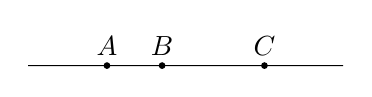
\begin{tikzpicture}
			\draw[fill=black] (0,0)--(1,0)node[above]{\(A\)}circle(1pt)
			--(1.7,0)node[above]{\(B\)}circle(1pt)
			--(3,0)node[above]{\(C\)}circle(1pt)
			--(4,0);
		\end{tikzpicture}
		\caption{直线上点的顺序}
		\label{figure:欧式几何.直线上点的顺序1}
	\end{figure}

	\item 对于两点\(A\)和\(B\)(如\cref{figure:欧式几何.直线上点的顺序2}),
	直线\(AB\)上恒至少有一点\(C\),使得\(B\)在\(A\)和\(C\)之间.
	\begin{figure}[ht]
		\centering
		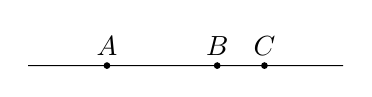
\begin{tikzpicture}
			\draw[fill=black] (0,0)--(1,0)node[above]{\(A\)}circle(1pt)
			--(2.4,0)node[above]{\(B\)}circle(1pt)
			--(3,0)node[above]{\(C\)}circle(1pt)
			--(4,0);
		\end{tikzpicture}
		\caption{直线上点的顺序}
		\label{figure:欧式几何.直线上点的顺序2}
	\end{figure}

	\item 一直线的任意三点中,至多有一点在其他两点之间.
\end{enumerate}
\end{axiom}

在上述三条{\bf 直线顺序公理}之外,还需要一条{\bf 平面顺序公理}.

\begin{axiom}[顺序公理II]\label{axiom:欧式几何.顺序公理2}
考虑一直线\(l\)上的两点\(A\)和\(B\).
我们把这一对点\(A\)和\(B\)确定的介于它们的点的集合叫做一条\DefineConcept{线段},记作\(AB\)(或\(BA\)).
在\(A\)和\(B\)之间的点叫做线段\(AB\)的点,或线段\(AB\)的\DefineConcept{内点};
\(A\)和\(B\)叫做线段\(AB\)的\DefineConcept{端点};
直线\(l\)上的其他点叫做线段\(AB\)的\DefineConcept{外点}.
\begin{enumerate}
	\setcounter{enumi}{3}
	\item 设\(A\)、\(B\)和\(C\)是不在同一直线上的三点,
	\(l\)是平面\(ABC\)上的一直线,
	但\(l\)不通过\(A,B,C\)这三点中的任一点
	(如\cref{figure:欧式几何.平面上点的顺序1}),
	若直线\(l\)通过线段\(AB\)的一点,则它必定也通过线段\(AC\)或线段\(BC\)的一点.
	\begin{figure}[ht]
		\centering
		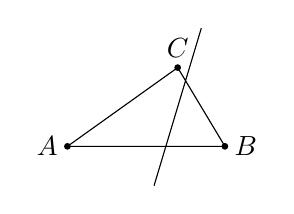
\begin{tikzpicture}
			\draw[fill=black] (-1,0)node[left]{\(A\)}circle(1pt)
			--(1,0)node[right]{\(B\)}circle(1pt)
			--(.4,1)node[above]{\(C\)}circle(1pt)--(-1,0)
			(.1,-.5)--(.7,1.5);
		\end{tikzpicture}
		\caption{平面上点的顺序}
		\label{figure:欧式几何.平面上点的顺序1}
	\end{figure}
\end{enumerate}
\end{axiom}
直观地说,\cref{axiom:欧式几何.顺序公理2} 说的就是:
若一直线“冲进”一个三角形的内部,它必定还要再“冲出”这个三角形.
易证:与线段\(AB\)相交的直线\(l\)不同时和\(AC,BC\)这两条线段都相交.

\subsection{关联公理和顺序公理的推论}
从\cref{axiom:欧式几何.关联公理,axiom:欧式几何.顺序公理1,axiom:欧式几何.顺序公理2} 能推证下列定理.
\begin{theorem}\label{theorem:欧式几何.定理3}
对于两点\(A\)和\(C\),直线\(AC\)上恒至少有一点\(D\),在\(A\)和\(C\)之间.
\begin{proof}
根据\cref{axiom:欧式几何.关联公理} 第3条,直线\(AC\)外存在一点\(E\);
根据\cref{axiom:欧式几何.顺序公理1} 第2条,直线\(AE\)上有一点\(F\),使得\(E\)在线段\(AF\)内.
根据\cref{axiom:欧式几何.顺序公理1} 第2条、第3条,直线\(FC\)上有一点\(G\),不在线段\(FC\)内.
根据\cref{axiom:欧式几何.顺序公理2} 第4条,直线\(EG\)必交线段\(AC\)于一点\(D\).
\end{proof}
\end{theorem}

\begin{theorem}\label{theorem:欧式几何.定理4}
一直线上的任意三点\(A,B,C\)中,必有一点且只有一点在其他两点之间.
\begin{proof}
设\(A\)不在\(B\)和\(C\)之间,而且\(C\)不在\(A\)和\(B\)之间.
用直线连接\(B\)和直线\(AC\)外一点\(D\).
根据\cref{axiom:欧式几何.顺序公理1} 第2条,能在直线\(BD\)上取一点\(G\),使得\(D\)在\(B\)和\(G\)之间.
对于三角形\(BCG\)和直线\(AD\)应用\cref{axiom:欧式几何.顺序公理2} 第4条,可知直线\(AD\)通过线段\(CG\)内的一点\(E\);
同理可知直线\(CD\)通过线段\(AG\)内一点\(F\).
对于三角形\(AEG\)和直线\(CF\)应用\cref{axiom:欧式几何.顺序公理2} 第4条,可知\(D\)在\(A\)和\(E\)之间;
再对于三角形\(AEC\)和直线\(BG\)应用\cref{axiom:欧式几何.顺序公理2} 第4条,即证得\(B\)在\(A\)和\(C\)之间.
\end{proof}
\end{theorem}

\begin{theorem}\label{theorem:欧式几何.定理5}
一直线上的任意四点\(A,B,C,D\),使得点\(B\)既在\(A\)和\(C\)之间,又在\(A\)和\(D\)之间;
而且点\(C\)既在\(A\)和\(D\)之间,又在\(B\)和\(D\)之间.
\end{theorem}

\begin{corollary}\label{theorem:欧式几何.定理6}
一直线上的任意有限个点\(A,B,C,\dotsc,K\),
使得点\(B\)在\(A\)和\(C\),或和\(D\),或和\(E\),……,或和\(K\)之间;
而且点\(C\)在\(A\)(或\(B\))和\(D\),或和\(E\),……,或和\(K\)之间;以此类推.
\end{corollary}

\begin{corollary}\label{theorem:欧式几何.定理7}
一直线上任意两点之间恒有无限多个点.
\end{corollary}

\begin{theorem}\label{theorem:欧式几何.定理8}
一平面\(\gamma\)上的任一直线\(l\)将该平面上其余的点分为具有下述性质的两个区域:
一个区域的任一点\(A\)与另一区域的任一点\(B\)所决定的线段\(AB\)内,
必含有直线\(l\)的一点(如\cref{figure:欧式几何.直线l分平面为两个区域});
而同一个区域的任意两点\(A\)和\(A'\)所决定的线段\(AA'\)内,不含有直线\(l\)的点.
\begin{figure}[ht]
\centering
\begin{tikzpicture}
\draw (-2,0)--(2,0)node[right]{\(l\)}
(.5,-1)node[right]{\(B\)}--(-.5,.5)node[left]{\(A\)}--(.3,1)node[right]{\(A'\)};
\end{tikzpicture}
\caption{直线\(l\)分平面为两个区域}
\label{figure:欧式几何.直线l分平面为两个区域}
\end{figure}
\end{theorem}

\begin{definition}
我们说\(A\)和\(A'\)这两点在平面\(\gamma\)上直线\(l\)的\DefineConcept{同侧}%
(如\cref{figure:欧式几何.直线l分平面为两个区域}),
而\(A\)和\(B\)这两点在平面\(\gamma\)上直线\(l\)的\DefineConcept{异侧}.
\end{definition}

\begin{definition}
设\(A,A',O\)和\(B\)是一直线\(l\)上的四点(如\cref{figure:欧式几何.射线}),
而\(O\)在\(A\)和\(B\)之间,但不在\(A\)和\(A'\)之间.
我们称“\(A\)和\(A'\)这两点在\(l\)上点\(O\)的\DefineConcept{同侧}”,
而称“\(A\)和\(B\)这两点在\(l\)上点\(O\)的\DefineConcept{异侧}”.

直线\(l\)上点\(O\)的同侧的点的全体,叫做从点\(O\)起始的一条\DefineConcept{射线};
因此一直线的每一点把这直线分成两条射线.
\begin{figure}[ht]
\centering
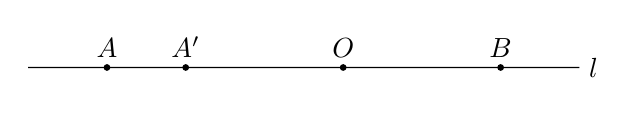
\begin{tikzpicture}
\draw[fill=black] (-3,0)--(-2,0)node[above]{\(A\)}circle(1pt)
--(-1,0)node[above]{\(A'\)}circle(1pt)
--(1,0)node[above]{\(O\)}circle(1pt)
--(3,0)node[above]{\(B\)}circle(1pt)--(4,0)node[right]{\(l\)};
\end{tikzpicture}
\caption{射线}
\label{figure:欧式几何.射线}
\end{figure}
\end{definition}

\begin{definition}
若干条首尾相连的线段\(AB,BC,CD,\dotsc,KL\)的集合叫做一条\DefineConcept{折线段},
它连结\(A\)和\(L\)这两点.
为求简便,可将这条折线段记为\(ABCD \dotso KL\).
线段\(AB,BC,CD,\dotsc,KL\)的内点和端点都叫做这条折线段的点.
点\(A\)和点\(L\)称为“折线段的\DefineConcept{端点}”.

若折线段\(ABCD \dotso KL\)的顶点\(A,B,C,D,\dotsc,K,L\)都在同一平面上,
且它的端点\(L\)和\(A\)是同一个点,
则这条折线段就叫做一个\DefineConcept{多边形},
记为\(ABCD \dotso K\).
线段\(AB,BC,CD,\dotsc,KA\)叫做“多边形的\DefineConcept{边}”.
点\(A,B,C,D,\dotsc,K\)叫做“多边形的\DefineConcept{顶点}”.

若一个多边形有三个顶点,
则称之为\DefineConcept{三角形}.
设三角形的三个顶点分别为\(A\)、\(B\)、\(C\),
则可将其表记为以下六个符号中的任意一个:
\[
\begin{split}
\triangle ABC, \qquad
\triangle ACB, \qquad
\triangle BAC, \\
\triangle BCA, \qquad
\triangle CAB, \qquad
\triangle CBA.
\end{split}
\]

若一个多边形有\(n\ (n>3)\)个顶点,
则称之为\(n\) \DefineConcept{边形}.

若一个多边形的顶点各各不同,
它的任一边内不含有顶点,
且它的任意两边无公共点,
这个多边形就叫做\DefineConcept{简单多边形}.
\end{definition}

根据\cref{theorem:欧式几何.定理8} 可以推出下列两条推论:
\begin{theorem}\label{theorem:欧式几何.定理9}
一平面\(\alpha\)上的每一个简单多边形,
把平面\(\alpha\)上其余点%
(即平面\(\alpha\)上的,
而不在这多边形的边上的点)%
分为\DefineConcept{内域}和\DefineConcept{外域}两个区域.
这两个区域具有如下性质:
\begin{enumerate}
	\item 若\(A\)是“内域的一个点(内点)”,
	而且\(B\)是“外域的一个点(外点)”,
	则平面\(\alpha\)上任意一条连接\(A\)和\(B\)的折线段,
	至少和多边形有一公共点.

	\item 若\(A\)和\(C\)是内点,
	而\(B\)和\(D\)是外点,
	则在平面\(\alpha\)上恒有连接\(A\)和\(C\)的折线段,
	和连接\(B\)和\(D\)的折线段,
	它们都和多边形无公共点.

	\item 平面\(\alpha\)上存在全含于外域的直线,
	而不存在全含于内域的直线.
\end{enumerate}
\end{theorem}

\begin{theorem}\label{theorem:欧式几何.定理10}
每一平面\(\alpha\)把空间中其余点分为具有下述性质的两个区域:
\begin{enumerate}
	\item 一区域的任一点\(A\)和另一区域的任一点\(B\)所决定的线段\(AB\)内,必含有\(\alpha\)的一点.
	\item 同一区域的任意两点\(A\)和\(C\)所决定的线段\(AC\)内,恒不含有\(\alpha\)的点.
\end{enumerate}
\end{theorem}

\begin{definition}
在\cref{theorem:欧式几何.定理10} 的条件下,
我们说“\(A\)和\(C\)这两点在空间中平面\(\alpha\)的\DefineConcept{同侧}”,
说“\(A\)和\(B\)这两点在空间中平面\(\alpha\)的\DefineConcept{异侧}”.
\end{definition}

\subsection{第三组公理:合同公理}
本组公理规定“合同”这个概念,利用它就可以规定运动的概念.

我们首先介绍角的概念.
\begin{definition}\label{definition:欧式几何.几何元素.角}
设\(\alpha\)是任意平面,
而且\(h\)和\(k\)是\(\alpha\)上的、%
从一点\(A\)起始的、%
不属于同一直线的%
两条射线,
我们把这一对射线\(h\)和\(k\)所成的射线组叫做一个\DefineConcept{角},
记作\(\angle(h,k)\)或\(\angle(k,h)\).
称射线\(h\)和\(k\)为这个角的\DefineConcept{边}.
称点\(A\)为这个角的\DefineConcept{顶点}.

如果在\(h\)上任取一点记为\(B\),在\(k\)上任取一点记为\(C\),
那么也称角\(\angle(h,k)\)为\(\angle BAC\)或\(\angle A\).
不致混淆时,也可以用小写希腊字母表记角.

记射线\(h\)所在的直线为\(p\),射线\(k\)所在的直线为\(q\).
射线\(h\)与\(k\)(包括点\(A\))把平面\(\alpha\)上其余点分成两个区域:
在\(q\)的\(h\)侧(即\(h\)的点所在的那一侧)的,且%
在\(p\)的\(k\)侧(即\(k\)的点所在的那一侧)的区域,
叫做“角\(\angle(h,k)\)的\DefineConcept{内部}”,
或者说是在\DefineConcept{角内};
其他区域叫做“角\(\angle(h,k)\)的\DefineConcept{外部}”,
或者说是在\DefineConcept{角外}.
\end{definition}

\begin{property}
根据第一组和第二组公理,
易知任意角(不妨设为交于点\(A\)的射线\(h\)、\(k\)所成的角,即\(\angle(h,k)\))具有以下性质:
\begin{enumerate}
\item 角内、角外两个区域各含有点,连结角内两点的线段完全在角内.
\item 若点\(H\)在射线\(h\)上,点\(K\)在射线\(k\)上,则线段\(HK\)完全在角内.
\item 一条从点\(A\)起始的射线,要么完全在角内,要么完全在角外.
\item 一条完全在角内的射线与线段\(HK\)有交点.
\item 若\(B\)是一个区域的一点,而且\(C\)是另一个区域的一点,
则每一条连接\(B\)和\(C\)的折线段,要么通过点\(A\),要么与\(h\)或\(k\)至少有一个交点;
反之,若\(B\)和\(D\)是同一个区域的两点,则恒有一条连接\(B\)和\(D\)的折线段,
它既不通过点\(A\),又与\(h\)、\(k\)无交点.
\end{enumerate}
\end{property}


\begin{axiom}[合同公理]\label{axiom:欧式几何.合同公理}
线段与线段之间、角与角之间都有一定的相互关系,我们用“合同”或“相等”这个词来描述.
\begin{enumerate}
\item 设\(A\)和\(B\)是直线\(a\)上的两点,
\(P\)是直线\(b\)上的点,
而且给定了直线\(b\)上\(P\)的一侧,
则在直线\(b\)上\(P\)的这一侧,
恒有一点\(Q\),
使得线段\(AB\)和线段\(PQ\)合同.
我们将上述关系记为\(AB \equiv PQ\).

\item 若两线段\(PQ\)和\(MN\)都和线段\(AB\)合同,
则\(PQ\)和\(MN\)也合同.

\item 设两线段\(AB\)和\(BC\)在同一直线\(a\)上,无公共点,
而且两线段\(PQ\)和\(QR\)在同一直线\(b\)上,亦无公共点.
若\(AB \equiv PQ\)且\(BC \equiv QR\),
则\(AC \equiv PR\).

\item 设给定了一个平面\(\alpha\)上的一个角\(\angle(h,k)\),
一平面\(\beta\)上的一直线\(b\),
和在\(\beta\)上\(b\)的一侧.
设\(p\)是\(b\)上的、从点\(B\)起始的一条射线,
则平面\(\beta\)上恰有一条射线\(q\),
使得\(\angle(h,k)\)与\(\angle(p,q)\)合同,
而且使得\(\angle(p,q)\)的内部在\(b\)的这给定了的一侧.
我们将上述关系记为\(\angle(h,k) \equiv \angle(p,q)\).

\item 若两个三角形\(ABC\)和\(PQR\)有下列合同式
\[
AB \equiv PQ, \qquad
AC \equiv PR, \qquad
\angle BAC \equiv \angle QPR,
\]
则也恒有合同式\footnote{%
只需要交换记号,还可以同时得到另一个合同式
\(\angle ACB \equiv \angle PRQ\)
也同时成立.
}
\[
\angle ABC \equiv \angle PQR.
\]
\end{enumerate}
\end{axiom}

我们在前面用点\(A\)、\(B\)所成的点组规定一条线段,并用\(AB\)或\(BA\)表示;
我们在线段的定义里,并不考虑这两点的顺序;
因此下列四个合同式的意义相同:
\[
AB \equiv PQ, \qquad
AB \equiv QP, \qquad
BA \equiv PR, \qquad
BA \equiv QP.
\]

如同线段我们不考虑它的方向,在角的定义中我们也不考虑旋转方向.
因此下列四个合同式的意义也相同:
\[
\angle(h,k) \equiv \angle(p,q), \qquad
\angle(h,k) \equiv \angle(q,p), \qquad
\angle(k,h) \equiv \angle(p,q), \qquad
\angle(k,h) \equiv \angle(q,p).
\]

\cref{axiom:欧式几何.合同公理} 第3条要求线段能够相加.

\cref{axiom:欧式几何.合同公理} 第4条可以表述为:
每一个角都能用唯一确定的方式迁移到一个给定了的平面上,
使得它沿着一条给定了的射线,并且在这射线的给定了的一侧.
藉此,我们直接保证了角的迁移的可能性与唯一性.

\cref{axiom:欧式几何.合同公理} 第1条、第2条、第3条只论及线段的合同,
因此可以叫做“第三组公理中的直线公理”.

\cref{axiom:欧式几何.合同公理} 第4条论及角的合同.
\cref{axiom:欧式几何.合同公理} 第5条则把线段的合同和角的合同这两个概念联系起来.
这两条概念论及平面几何的几何元素,
因此可以叫做“第三组公理中的平面公理”.

\cref{axiom:欧式几何.合同公理} 第1条要求线段平移的可能性,
但它还没有保证这种平移的唯一性.
只有结合\cref{axiom:欧式几何.合同公理} 第5条,
从角的迁移的唯一性出发予以证明.
具体地,我们应用反证法,
假设把线段\(PQ\)迁移到一条从\(A\)起始的射线上可以得到不同的两点\(B\)、\(D\);
在直线\(AB\)外取一点\(C\),于是有下列合同式
\[
AB \equiv AD, \qquad
AC \equiv AC, \qquad
\angle BAC \equiv \angle DAC;
\]
那么根据\cref{axiom:欧式几何.合同公理} 第5条,得
\[
\angle ACB \equiv \angle ACD;
\]
这和\cref{axiom:欧式几何.合同公理} 第4条中要求的角的迁移的唯一性矛盾,
因此线段平移也是唯一的.

\begin{property}
线段的合同关系具有自反性、对称性和传递性,即
\begin{enumerate}
\item {\bf 自反性},
\(AB \equiv AB\).

\item {\bf 对称性},
\(AB \equiv PQ \implies PQ \equiv AB\)
\footnote{%
正因线段的合同关系具有对称性,
我们才能说“某两条线段互相合同”.
}.

\item {\bf 传递性},
\(AB \equiv PQ \land PQ \equiv MN \implies AB \equiv MN\).
\end{enumerate}
\end{property}

\begin{property}
角的合同关系具有自反性、对称性和传递性,即
\item {\bf 自反性},
\(\angle(h,k) \equiv \angle(h,k)\).

\item {\bf 对称性},
\(\angle(h,k) \equiv \angle(p,q)
\implies
\angle(p,q) \equiv \angle(h,k)\).

\item {\bf 传递性},
\(\angle(h,k) \equiv \angle(m,n)
\land
\angle(m,n) \equiv \angle(p,q)
\implies
\angle(h,k) \equiv \angle(p,q)\).
\end{property}
角的合同关系的自反性是显然的,
至于它的对称性、传递性和可加性,
则留待以后予以证明.

\subsection{合同公理的推论}
\begin{definition}
两角共顶点,共一边,而且不公共的两边合成一条直线的,叫做\DefineConcept{邻补角}.
\end{definition}
\begin{definition}
两角共顶点,而且它们的边合成两条直线的,叫做\DefineConcept{对顶角}.
\end{definition}
\begin{definition}
一个角和它的邻补角合同的,叫做\DefineConcept{直角}.
\end{definition}

\begin{theorem}\label{theorem:欧式几何.定理11}
若一个三角形中的两边合同,和这两边相对的两角就也合同\footnote{%
换言之,等腰三角形的底角相等.
}.
\end{theorem}

\begin{definition}
若两个三角形\(ABC\)和\(PQR\)满足下列所有的合同式
\[
\begin{split}
AB \equiv PQ, \qquad
AC \equiv PR, \qquad
BC \equiv QR, \\
\angle A \equiv \angle P, \qquad
\angle B \equiv \angle Q, \qquad
\angle C \equiv \angle R,
\end{split}
\]
就说“三角形\(ABC\)合同于三角形\(PQR\)”,
或者说“三角形\(ABC\)和三角形\(PQR\)是全等三角形”,
或者说“三角形\(ABC\)、\(PQR\)全等”,
记为\(\triangle ABC \cong \triangle PQR\).
\end{definition}

\begin{theorem}[三角形的合同定理1]\label{theorem:欧式几何.定理12}
若两个三角形\(ABC\)、\(PQR\)有下列合同式
\[
AB \equiv PQ, \qquad
AC \equiv PR, \qquad
\angle A \equiv \angle P,
\]
则\(\triangle ABC \cong \triangle PQR\).
\end{theorem}

\begin{theorem}[三角形的合同定理2]\label{theorem:欧式几何.定理13}
若两个三角形\(ABC\)、\(PQR\)有下列合同式
\[
AB \equiv PQ, \qquad
\angle A \equiv \angle P,
\angle B \equiv \angle Q,
\]
则\(\triangle ABC \cong \triangle PQR\).
\end{theorem}

\begin{theorem}\label{theorem:欧式几何.定理14}
设\(\angle ABC\)的邻补角为\(\angle CBD\),
\(\angle PQR\)的邻补角为\(\angle RQS\).
若\(\angle ABC \equiv \angle PQR\),
则\(\angle CBD \equiv \angle RQS\).
\end{theorem}

\begin{corollary}\label{theorem:欧式几何.对顶角合同}
任意一个角和它的对顶角合同.
\end{corollary}

\begin{corollary}\label{theorem:欧式几何.直角存在}
直角存在.
\begin{proof}
把任意一个角迁移到沿着一条从点\(O\)起始的射线\(OA\),
而且迁移到这射线的两侧.
在新得到的这两个角的另外两条边上,
取线段\(OB \equiv OC\),
线段\(BC\)交射线\(OA\)于一点\(D\).

若点\(D\)就是点\(O\),
\(\angle BOA\)和\(\angle COA\)是合同的邻补角,所以是直角.

若点\(D\)在射线\(OA\)上,
或在与\(OA\)恰好反向的射线上,
总有\(\angle DOB \equiv \angle DOC\);
根据\cref{axiom:欧式几何.合同公理} 第2条,
每一条线段都和它自己合同,即\(OD \equiv OD\);
再根据\cref{axiom:欧式几何.合同公理} 第5条,
就有\(\angle ODB \equiv \angle ODC\).
\end{proof}
\end{corollary}

\begin{theorem}\label{theorem:欧式几何.定理15}
设\(h\)、\(k\)和\(l\)是一平面\(\alpha\)上的、从一点\(M\)起始的三条射线,
而且\(p\)、\(q\)和\(r\)是一平面\(\beta\)上的、从一点\(N\)起始的三条射线;%
又设\(h\)和\(k\)分别在\(l\)的同侧(或异侧),
且\(p\)和\(q\)也分别在\(r\)的同侧(或异侧).
若
\[
\angle(h,l) \equiv \angle(p,r)
\quad\text{且}\quad
\angle(k,l) \equiv \angle(q,r),
\]
则
\[
\angle(h,k) \equiv \angle(p,q).
\]
\end{theorem}

\begin{theorem}\label{theorem:欧式几何.定理16}
设平面\(\alpha\)上的\(\angle(h,k)\)合同于平面\(\beta\)上的\(\angle(p,q)\),
而且\(l\)是平面\(\alpha\)上的、从\(\angle(h,k)\)的顶点起始的、在\(\angle(h,k)\)角内的一条射线.
这时平面\(\beta\)上恒恰有一条从\(\angle(p,q)\)的顶点起始的、在\(\angle(p,q)\)角内的一条射线\(r\),
使得
\[
\angle(h,l) \equiv \angle(p,r), \qquad
\angle(k,l) \equiv \angle(q,r).
\]
\end{theorem}

\begin{theorem}\label{theorem:欧式几何.定理17}
若两点\(C\)和\(D\)在直线\(AB\)的异侧,
而且\(AC \equiv AD\)、\(BC \equiv BD\),
则\(\angle ABC \equiv \angle ABD\).
\end{theorem}

\begin{theorem}[三角形的合同定理3]\label{theorem:欧式几何.定理18}
若两个三角形\(ABC\)和\(PQR\)的每对对应边合同,即
\[
AB \equiv PQ, \qquad
AC \equiv PR, \qquad
BC \equiv QR,
\]
则\(\triangle ABC \cong \triangle PQR\).
\end{theorem}

\begin{theorem}\label{theorem:欧式几何.定理19}
若两个角\(\angle(a,b)\)和\(\angle(c,d)\)都合同于第三个角\(\angle(e,f)\),
则\(\angle(a,b)\)也合同于\(\angle(c,d)\).
\end{theorem}
由此,我们证明了角的合同关系具有对称性、传递性.

现在我们就可以比较角的大小了.

\begin{theorem}\label{theorem:欧式几何.定理20}
如\cref{figure:欧式几何.图20},
给定任意两个角\(\angle(h,k)\)和\(\angle(p,r)\).
设迁移\(\angle(h,k)\)到沿着\(p\),而且在\(p\)的\(r\)侧时,所得到的射线是\(q\);
又迁移\(\angle(p,r)\)到沿着\(h\),而且在\(h\)的\(k\)侧时,所得到的射线是\(l\);
这时,若\(q\)在\(\angle(p,r)\)内,则\(l\)在\(\angle(h,k)\)外.
反之也成立.
\end{theorem}

\begin{figure}[ht]
	\centering
	\begin{tikzpicture}
		\pgfmathsetmacro{\r}{3}
		\begin{scope}
			\draw(0,0)--(\r,0)node[right]{\(h\)};
			\pgfmathsetmacro{\kx}{\r*cos(45)}
			\pgfmathsetmacro{\ky}{\r*sin(45)}
			\draw(0,0)--(\kx,\ky)node[right]{\(k\)};
			\pgfmathsetmacro{\lx}{\r*cos(60)}
			\pgfmathsetmacro{\ly}{\r*sin(60)}
			\draw(0,0)--(\lx,\ly)node[above]{\(l\)};
		\end{scope}
		\begin{scope}[xshift=6cm]
			\draw(0,0)--(\r,0)node[right]{\(p\)};
			\pgfmathsetmacro{\kx}{\r*cos(45)}
			\pgfmathsetmacro{\ky}{\r*sin(45)}
			\draw(0,0)--(\kx,\ky)node[right]{\(q\)};
			\pgfmathsetmacro{\lx}{\r*cos(60)}
			\pgfmathsetmacro{\ly}{\r*sin(60)}
			\draw(0,0)--(\lx,\ly)node[above]{\(r\)};
		\end{scope}
	\end{tikzpicture}
	\caption{}
	\label{figure:欧式几何.图20}
\end{figure}

\begin{definition}
在\cref{theorem:欧式几何.定理20} 中,
若\(q\)在\(\angle(p,r)\)内,则称“\(\angle(h,k)\)小于\(\angle(p,r)\)”,记为\(\angle(h,k) < \angle(p,r)\).
若\(q\)在\(\angle(p,r)\)外,则称“\(\angle(h,k)\)大于\(\angle(p,r)\)”,记为\(\angle(h,k) > \angle(p,r)\).
\end{definition}

因此,两个角\(\alpha,\beta\)恒恰适合以下三种情形之一:
\begin{itemize}
	\item \(\alpha<\beta\)和\(\beta>\alpha\).
	\item \(\alpha\equiv\beta\).
	\item \(\alpha>\beta\)和\(\beta<\alpha\).
\end{itemize}

角的大小的比较有传递性.
若有下列三种情形
\begin{itemize}
	\item \(\alpha>\beta,\beta>\gamma\),
	\item \(\alpha>\beta,\beta\equiv\gamma\),
	\item \(\alpha\equiv\beta,\beta>\gamma\),
\end{itemize}
之一,则\[
	\alpha>\gamma.
\]

\begin{theorem}\label{theorem:欧式几何.定理21}
所有的直角都互相合同.
\end{theorem}

\begin{definition}
一个角大于它的邻补角的,也就是大于一直角的,叫做\DefineConcept{钝角};
小于它的邻补角的,也就是小于一直角的,叫做\DefineConcept{锐角}.
\end{definition}

\begin{definition}
\(\triangle ABC\)的\(\angle ABC\)、\(\angle BCA\)和\(\angle CAB\)
叫做这个三角形的\DefineConcept{内角},简称为这个三角形的\DefineConcept{角};
它们的邻补角叫做这个三角形的\DefineConcept{外角}.
\end{definition}

\begin{theorem}[外角定理]\label{theorem:欧式几何.定理22}
在三角形中,一个外角大于其任一不相邻的内角.
\end{theorem}

下列定理是外角定理的重要推论.

\begin{theorem}\label{theorem:欧式几何.定理23}
在三角形中,长边所对的角大于短边所对的角.
\end{theorem}

\begin{theorem}\label{theorem:欧式几何.定理24}
若三角形有两角合同,则有两边合同.
\end{theorem}
这是\cref{theorem:欧式几何.定理11} 的逆定理,
也是\cref{theorem:欧式几何.定理23} 的直接推论.

从\cref{theorem:欧式几何.定理22},
还能很简单地证得下述对三角形的合同定理二的补充.
\begin{theorem}\label{theorem:欧式几何.定理25}
若\(\triangle ABC\)和\(\triangle DEF\)有下列合同式\[
	AB \equiv DE, \qquad
	\angle A \equiv \angle D, \qquad
	\angle C \equiv \angle F,
\]
则这两个三角形合同.
\end{theorem}

\begin{theorem}\label{theorem:欧式几何.定理26}
每一线段都能二等分.
\end{theorem}

类似地,从\cref{theorem:欧式几何.定理11} 和\cref{theorem:欧式几何.定理26},能直接推证下列事实:
\begin{theorem}
每一角都能二等分.
\end{theorem}

合同的概念可以推广应用到任意的图形上去.

\begin{definition}
设\(A,B,C,D,\dotsc,K,L\)是直线\(\alpha\)上的一个点列,
\(A',B',C',D',\dotsc,K',L'\)是直线\(\alpha'\)上的一个点列,
而且所有的对应线段都两两合同,
那么称这两个点列互相合同.
\(A\)和\(A'\)、\(B\)和\(B'\),一直到\(L\)和\(L'\),叫做这\emph{合同点列}的对应点.
\end{definition}

\begin{theorem}\label{theorem:欧式几何.定理27}
两个合同的点列的点的顺序相同.
\end{theorem}

\begin{definition}
任意有限个点叫做一个\DefineConcept{图形}.
一个图形的点,若都在一个平面上,这图形就叫做一个\DefineConcept{平面图形}.
\end{definition}

两个图形的点之间若有一个一一对应的关系,
使得由此规定的每对对应的线段都互相合同,
且每对对应的角都互相合同,
那么这两个图形合同.

由\cref{theorem:欧式几何.定理14}
和\cref{theorem:欧式几何.定理27},
可知合同图形有下述性质:
若一个图形中的三个点在一条直线上,
则每一个和它合同图形中的对应的三个点也在一条直线上.
合同图形中的、对应平面上的对应点,
对于对应直线而言的顺序相同;
对应直线上的对应点顺序也相同.

平面的和空间的最普遍的合同定理如下:
\begin{theorem}\label{theorem:欧式几何.定理28}
设\((A,B,C,\dotsc,L)\)
和\((A',B',C',\dotsc,L')\)
是两个合同的平面图形.
若\(P\)是第一个图形的平面上的一点,
则第二个图形的平面上恒有一点\(P'\)存在,
使得\((A,B,C,\dotsc,L,P)\)
和\((A',B',C',\dotsc,L',P')\)还是合同的图形.
若\((A,B,C,\dotsc,L)\)至少含有不在同一条直线上的三点,
则\(P'\)只有一个可能的作法.
\end{theorem}

\begin{theorem}\label{theorem:欧式几何.定理29}
设\((A,B,C,\dotsc,L)\)
和\((A',B',C',\dotsc,L')\)
是两个合同的图形.
若\(P\)是任意一点,
则恒有一点\(P'\)存在,
使得\((A,B,C,\dotsc,L,P)\)
和\((A',B',C',\dotsc,L',P')\)还是合同的图形.
若\((A,B,C,\dotsc,L)\)至少含有不在同一平面上的四点,
则\(P'\)只有一个可能的作法.
\end{theorem}

\cref{theorem:欧式几何.定理29} 说出了所有关于合同的空间事实,
因此,空间中运动的性质,都是上述的直线的和平面的五条合同公理(结合着第一组和第二组公理)的推论.

\subsection{第四组公理:平行公理}
设\(\alpha\)是任一平面,
\(a\)是\(\alpha\)上的任一直线,
而且\(A\)是\(\alpha\)上的、但不在\(a\)上的一点,
在\(\alpha\)上作一直线\(c\),
通过\(A\)且和\(a\)相交,
再在\(\alpha\)上作一直线\(b\),通过\(A\),
且使得\(c\)交\(a\)和\(b\)于相等的同位角.
从\hyperref[theorem:欧式几何.定理22]{外角定理},
易知\(a\)和\(b\)这两直线无公共点,这就是说,
在一平面\(\alpha\)上,而且通过一直线\(a\)外的一点\(A\),
恒有一直线不和\(a\)相交.

现在可将平行公理叙述如下:
\begin{axiom}[平行公理、欧几里得公理]\label{axiom:欧式几何.平行公理}
设\(a\)是任一直线,\(A\)是\(a\)外的任一点.
在\(a\)和\(A\)所决定的平面上,
至多有一条直线通过\(A\),而且不和\(a\)相交.
\end{axiom}

根据上文和平行公理,我们知道:
在\(a\)和\(A\)所决定的平面上,恰有一直线,通过\(A\)且不和\(a\)相交,
我们把这条直线叫做“通过\(A\)的\(a\)的\DefineConcept{平行直线}”.

平行公理和下述的要求等价:
如果一平面上的\(a\)和\(b\)两直线都不和这平面上的第三条直线\(c\)相交,
那么\(a\)和\(b\)也不相交.

事实上,如果\(a\)和\(b\)有一公共点\(A\),那么在同一平面上,
就有了\(a\)和\(b\)这两条直线,都通过\(A\)而且不和\(c\)相交.
这和平行公理矛盾.
反之,从上述要求,也易推得平行公理.

平行公理是一条平面公理.
它的引入,使得几何的基础大大地简单化了,也使得几何的构造容易得多了.

例如,在合同公理之外,再加上平行公理,不难得到下列熟知的事实:
\begin{theorem}\label{theorem:欧式几何.定理30}
若两平行直线被第三条直线所截,则同位角合同,内错角也合同;
反之,若同位角合同,或内错角合同,则前两直线平行.
\end{theorem}

\begin{theorem}\label{theorem:欧式几何.定理31}
三角形的三个内角的和等于两个直角的和.
\end{theorem}
\begin{figure}[ht]
	\centering
	\begin{tikzpicture}
		\coordinate (A) at (0,0);
		\coordinate (B) at (4,0);
		\coordinate (C) at (3,2);
		\coordinate (P) at (2,2);
		\coordinate (Q) at (4,2);
		\draw (A)node[left]{\(A\)}
				-- (B)node[right]{\(B\)}
				-- (C)node[above]{\(C\)} -- (A);
		\draw (P)node[left]{\(P\)} -- (Q)node[right]{\(Q\)};
		\draw pic[draw=blue,angle radius=5mm]{angle=B--A--C}
				pic[draw=blue,angle radius=6mm]{angle=B--A--C}
				pic[draw=blue,angle radius=5mm]{angle=P--C--A}
				pic[draw=blue,angle radius=6mm]{angle=P--C--A}
				pic[draw=orange,angle radius=4mm]{angle=C--B--A}
				pic[draw=orange,angle radius=4mm]{angle=B--C--Q};
	\end{tikzpicture}
	\caption{}
	\label{figure:欧式几何.三角形内角和等于平角}
\end{figure}

\begin{definition}
设\(M\)是一平面\(\alpha\)上的任一点.
考虑\(\alpha\)上的所有的那些点\(A\),
它们使线段\(MA\)都互相合同的.
这种点\(A\)的全体叫做一个\DefineConcept{圆},
点\(M\)叫做“这个圆的\DefineConcept{中心}”,简称\DefineConcept{圆心}.
\end{definition}

根据这个定义,我们容易从第三组和第四组公理,推证关于圆的若干熟知的定理.
特别是下述的定理:
通过不在同一条直线上的三点,能作一圆;
关于同一条弦上的圆周角合同的定理;
关于内接于圆的一个四边形的角的定理.

\subsection{第五组公理:连续公理}

\begin{axiom}[连续公理]
关于线段、角的度量,有如下公理:
\begin{enumerate}
	\item (度量公理,阿基米德公理).
	若\(AB\)和\(CD\)是任意两线段,则必存在一个数\(n\)使得沿\(A\)到\(B\)的射线上,
	自\(A\)作首尾相接的\(n\)个线段\(CD\),必将越过\(B\)点.
	\item (直线完备公理).
	一直线上的点集联通其顺序关系与合同关系不可能再这样扩充,
	使得这直线上原来元素之间所具有的关系,
	从第一组、第二组、第三组公理所推出的直线顺序与合同的基本性质\footnote{%
	所谓“基本性质”是指第二组第一至三条公理和\cref{theorem:欧式几何.定理5} 中所叙述的顺序性质,
	以及第三组第一至第三条公理中所叙述的合同性质连同迁移线段的唯一性.}
	以及度量公理都仍旧保持\footnote{%
	所谓“仍旧保持”是指,当点集扩充后,顺序关系及合同关系也将延续到扩充后的点集中去.
	我们注意到第一组第三条公理在各种扩充后,不言而喻地仍然保持,
	至于在所考虑的扩充下,\cref{theorem:欧式几何.定理3} 仍能成立,
	则是保持阿基米德公理的结果.}.
\end{enumerate}
\end{axiom}

完备公理中所要求保持的诸公理之一是阿基米德公理,
这时完备公理从本质上能以建立所不可缺少的一个条件.
其实我们能够证明:
若直线上的一个点集能满足上面所列举的关于顺序公理和定理以及合同公理和定理,
这点集就恒能够增加新点,使扩充后的点集还满足这里所提到的诸公理;
也就是说,如果一条完备公理,只要求保持这里所提到的诸公理和定理,
但不要求保持阿基米德公理或一条等价的公理,就要产生矛盾.

这两条连续公理都是直线公理.

下面所述更普遍的定理,主要根据直线完备公理.
\begin{theorem}[完备定理]\label{theorem:欧式几何.定理32}
几何元素(即点、直线、平面)形成一个集合,
它在保持关联公理、顺序公理、合同公理和阿基米德公理,
从而更不用说,在保持全体公理的条件之下,
不可能经由点、直线和平面再行扩充.
\end{theorem}

完备定理还能表成较强的形式.
也就是在完备定理内缩要求保持的诸公理中,有些并不是绝对需要的,为了定理能够成立,
重要的倒是在所要求保持的诸公理中包含有第一组第七条公理.
其实我们能证明:
对于满足第一至第第五组公理的元素集合,恒能给添加新的点、直线和平面,
使得扩充后的心机和能满足除去第一组第七条公理之外的全体公理;
这就是说,一条完备定理若不包含第一组第七条公理或一条等价的公理,就将引出矛盾.

完备公理不是阿基米德公理的一个推论.
实际上,只有阿基米德公理,连同第一至第四组公理,
并不足以证明我们的几何和通常的笛卡尔解析几何完全相同.
但是加上了完备公理(虽然这条公理并没有直接提到收敛的概念),
就能证明(相当于戴德金分割的)确界的存在,
和关于聚点存在的波尔查诺定理,
从而才证明欧式几何和笛卡尔几何相同.

从上文可见,连续的要求,在本质上,分成两个不同的部分:
阿基米德公理和完备公理;
前者的作用是替连续的要求做准备,
后者为完成整个公理系统作基础.

在本章后面的研究中,我们主要只用阿基米德公理作根据,而普遍地不假设完备公理.

\section{平面三角形}

\begin{theorem}
三角形内角和为\(\pi\).
\begin{proof}
设有\(\triangle ABC\).
过点\(C\)作平行于线段\(AB\)的直线\(PQ\).

由内错角相等,有\[
\angle{PCA} = \angle{CAB}, \quad \angle{QCB} = \angle{CBA},
\]又由\(\angle{PCA}+\angle{ACB}+\angle{QCB}=\pi\),可得\[
\angle{CAB}+\angle{ACB}+\angle{QCB}=\pi.
\qedhere
\]
\end{proof}
\end{theorem}

\begin{theorem}[正弦定理]
设任意三角形\(\triangle ABC\)的外接圆半径为\(R\),则\begin{equation}
\frac{a}{\sin A}
= \frac{b}{\sin B}
= \frac{c}{\sin C}
= 2R.
\end{equation}
\end{theorem}

\begin{theorem}[余弦定理]
设任意三角形\(\triangle ABC\),有\begin{equation}
c^2 = a^2 + b^2 - 2ab \cos C.
\end{equation}
\end{theorem}
可以看出,勾股定理是余弦定理的特殊情况,即当\(C = \frac{\pi}{2}\)时,有\(\cos C=0\),于是\(c^2 = a^2 + b^2\).

\begin{theorem}[摩尔外德公式]
%@see: https://arxiv.org/pdf/1808.08049.pdf
设任意三角形\(\triangle ABC\),则\begin{gather}
	\frac{a+b}{c}
	= \frac{\cos[(A-B)/2]}{\sin(C/2)}, \\
	\frac{a-b}{c}
	= \frac{\sin[(A-B)/2]}{\cos(C/2)}.
\end{gather}
\end{theorem}

\begin{theorem}[正切定理]
设任意三角形\(\triangle ABC\),有\begin{equation}
\frac{a-b}{a+b} = \frac{\tan[(A-B)/2]}{\tan[(A+B)/2]}.
\end{equation}
\end{theorem}

\section{圆}
\subsection{圆的概念}
\subsection{圆的性质}
\subsection{圆的周长\ 圆周率}
\begin{definition}
定义:圆的周长\(C\)与其直径\(2R\)之比称为\DefineConcept{圆周率},记作\(\pi\),即\[
\pi = \frac{C}{2R}.
\]
\end{definition}
由于圆周率是一个常数,那么已知圆的直径(或半径)可以求得圆的周长,而已知圆的周长可以求得圆的直径(或半径).

\begin{property}
给定圆上任意一段弧,若它的角度为\(\theta\),那么弧长为\(\theta r\).
\end{property}

\begin{corollary}
如下图,在单位圆上,当圆弧的角度\(\theta\)为锐角,即\(0<\theta<\pi/2\)时,\(\theta > x\). \begin{center}
\begin{tikzpicture}[scale=4]
%\draw[help lines, color=gray!30, dashed] (0,0) grid (1,1);
\pgfmathsetmacro{\u}{sqrt(3)/2}
\coordinate (O) at (0,0);
\coordinate (A) at (\u,0);
\coordinate (B) at (\u,1/2);
\draw (1,0)arc[start angle=0,end angle=30,radius=1]node[midway,right]{\(\theta\)} -- (0,0)node[midway,above left]{\(1\)} -- (1,0)
	(A) -- (B)node[midway,left]{\(x\)};
\draw pic["\(\theta\)",draw=orange,-,angle eccentricity=1.7,angle radius=5mm]{angle=A--O--B} pic[draw=gray,-,angle radius=0.3cm]{right angle=B--A--O};
\end{tikzpicture}
\end{center}
\end{corollary}

\section{平面凸多边形}
\begin{theorem}
设凸多边形的边数为\(n\),则其内角和为\((n-2)\pi\).
\end{theorem}
如图,在凸多边形内部任取一点\(P\),连接该点与凸多边形各顶点,可以得到\(n\)个三角形.
因为三角形内角和为\(\pi\),所以\(n\)个三角形内角和的总和为\(n\pi\),再减去各三角形\(\angle P\)之和\(2\pi\),可知凸\(n\)边形的内角和为\((n-2)\pi\).
\begin{center}
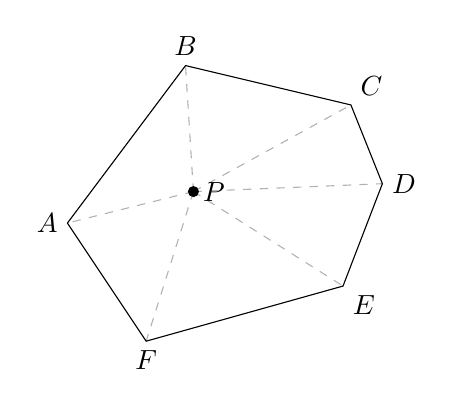
\begin{tikzpicture}
\coordinate (A1) at (0,2);
\coordinate (A2) at (1.5,4);
\coordinate (A3) at (3.6,3.5);
\coordinate (A4) at (4,2.5);
\coordinate (A5) at (3.5,1.2);
\coordinate (A6) at (1,0.5);
\coordinate (P) at (1.6,2.4);
\draw[dashed,color=black!30] (P)--(A1) (P)--(A2) (P)--(A3) (P)--(A4) (P)--(A5) (P)--(A6);
\draw (A1)node[left]{\(A\)}--(A2)node[above]{\(B\)}--(A3)node[above right]{\(C\)}--(A4)node[right]{\(D\)}--(A5)node[below right]{\(E\)}--(A6)node[below]{\(F\)}--(A1) (P)node[right]{\(P\)};
\fill (P)circle(2pt);
\end{tikzpicture}
\end{center}

\begin{theorem}
凸多边形的外角和为\(2\pi\).
\end{theorem}

\section{凸多面体}
\begin{theorem}[欧拉公式]
设凸多面体的顶点数、棱数、面数分别为\(V\)、\(E\)、\(F\),则有\[
V - E + F = 2.
\]
\end{theorem}

\begin{definition}
\DefineConcept{正凸多面体}(简称\DefineConcept{正多面体}),是指满足以下条件的凸多面体:
\begin{enumerate}
\item 正多面体的面由正多边形构成;
\item 正多面体的各个顶角相等;
\item 正多面体的各条棱长相等.
\end{enumerate}
\end{definition}

\begin{corollary}
正凸多面体只有5种:三四面体、正方体、正八面体、正十二面体、正二十面体.
\end{corollary}


\chapter{解析几何}
古希腊的毕达哥拉斯曾经提出“万物皆数”这一哲学观点,从这一章开始,我们研究如何利用代数方法研究几何问题.

在利用函数图像研究初等函数的性质时,我们产生了这么一个观念:
在平面上建立了平面直角坐标系以后,
平面上的点与数是一一对应的,
或说平面上的点与由实有序对\((x,y)\)一一对应.
几何图形是由点构成的集合,我们自然地想到能不能用数的集合来代表几何图形.
这就是解析几何的思想根源.



\section{向量及其线性运算}
解析几何最基本的方法是坐标法,即建立一个坐标系,使得点可以用有序对或元组来表示,
从而可以用方程表示图形,通过方程来研究图形的性质.
坐标法的优越性在于它利用了数可以进行运算的优点.
那么,能否把代数运算直接引入几何中来呢?什么样的几何对象能够做运算?

\subsection{向量的概念}
既有大小、又有方向的量,称为\DefineConcept{向量}或\DefineConcept{矢量}(vector).

与向量相对的,只有大小,没有方向的量,称为\DefineConcept{标量}(scalar).

我们通常用黑体小写拉丁字母(如\(\vb{a}\)、\(\vb{r}\)、\(\vb{v}\)、\(\vb{F}\)等),
或在小写拉丁字母上面加箭头(如\(\vec{a}\)、\(\vec{r}\)、\(\vec{v}\)、\(\vec{F}\)等)来表记向量.

在几何空间中,我们常用\DefineConcept{有向线段}(directed line segment)表示向量.
如\cref{figure:解析几何.有向线段} 所示,
对于一个给定的向量\(\vb{a}\),
我们可以用有向线段\(\vec{AB}\)来表示它,
其中用这条线段的长度\(\abs{AB}\)表示\(\vb{a}\)的大小,
用点\(A\)到点\(B\)的指向表示\(\vb{a}\)的方向.
我们把点\(A\)称为“有向线段\(\vec{AB}\)的\DefineConcept{起点}(initial point)”,
把点\(B\)称为“有向线段\(\vec{AB}\)的\DefineConcept{终点}(terminal point)”.
\begin{figure}[ht]
\centering
\begin{tikzpicture}[>=Stealth]
	\draw[->] (0,0)node[left]{\(A\)}--(3,1)node[right]{\(B\)}
		node[midway,above]{\(\vb{a}\)};
\end{tikzpicture}
\caption{有向线段}
\label{figure:解析几何.有向线段}
\end{figure}

规定长度相等、方向相同的有向线段表示同一个向量.

如\cref{figure:解析几何.有向线段的平移不变性} 所示,
若有向线段\(\vec{AB}\)表示向量\(\vb{a}\),
则\(\vec{AB}\)经过平行移动得到的有向线段\(\vec{CD}\)仍然表示向量\(\vb{a}\),
即\(\vb{a} = \vec{AB} = \vec{CD}\).
换言之,给定两条有向线段,如果其中一条经过平移可以让这两条有向线段的起点和终点分别完全重合,
那么这两条有向线段表示的是同一个向量.
\begin{figure}[ht]
\centering
\begin{tikzpicture}[>=Stealth]
	\draw[dashed] (0,0)--(5,0) (3,1)--(8,1);
	\draw[->] (0,0)node[left]{\(A\)}--(3,1)node[above left]{\(B\)}node[midway,above left]{\(\vb{a}\)};
	\draw[->] (5,0)node[below right]{\(C\)}--(8,1)node[right]{\(D\)};
\end{tikzpicture}
\caption{}
\label{figure:解析几何.有向线段的平移不变性}
\end{figure}

我们今后把向量的大小称为
“向量的\DefineConcept{长度}(length)”或“向量的\DefineConcept{模}(modulus)”,
记作\(\abs{\vb{a}}\).

如果两个向量\(\vb{a}\)和\(\vb{b}\)的长度相等、方向相同,
我们就说“\(\vb{a}\)和\(\vb{b}\)是\DefineConcept{相等}的”,
或者说“\(\vb{a}\)等于\(\vb{b}\)”,
记作\(\vb{a}=\vb{b}\);
否则,记\(\vb{a}\neq\vb{b}\).

长度为零的向量称为\DefineConcept{零向量}(zero vector),记作\(\vb{0}\).

看作有向线段时,零向量的起点和终点重合,所以它的方向可以看作是任意的、不确定的.

相对地,长度不为零的向量称为\DefineConcept{非零向量}(nonzero vector).

长度为1的向量称为\DefineConcept{单位向量}(identity vector),记作\(\vb{e}\).

任意给定一个向量\(\vb{a}\),与\(\vb{a}\)同向的单位向量记作\(\vb{a}^0\),
称其为“\(\vb{a}\)的\DefineConcept{方向}(direction)”.

任意给定一个向量\(\vb{a}\),
如果向量\(\vb{b}\)正好是与\(\vb{a}\)长度相等、方向相反的向量,
那么称“\(\vb{b}\)是\(\vb{a}\)的\DefineConcept{负向量}(negative vector)”,
记作\(-\vb{a}\).
例如,\(\vec{BA}\)是\(\vec{AB}\)的负向量,因此\(\vec{BA} = -\vec{AB}\).

\subsection{向量的加法}
我们知道,将与点\(A\)重合的点\(P\)移动到点\(B\)再移动到点\(C\)的结果是点\(P\)与点\(C\)重合.

\begin{definition}
%@see: 《解析几何》(丘维声) P2 定义1.1
对于向量\(\vb{a},\vb{b}\),
如\cref{figure:解析几何.向量相加的三角形法则} 所示,
作有向线段\(\vec{AB}\)表示\(\vb{a}\),
作有向线段\(\vec{BC}\)表示\(\vb{b}\),
把有向线段\(\vec{AC}\)表示的向量\(\vb{c}\)称为
“向量\(\vb{a}\)与\(\vb{b}\)的\DefineConcept{和}”,
记作\[
	\vec{AB}+\vec{BC}=\vec{AC}
	\quad\text{或}\quad
	\vb{c}=\vb{a}+\vb{b}.
\]
\end{definition}
由上述公式表示的向量加法规则通常称为\DefineConcept{三角形法则}(triangle law).
除此以外,我们还有\DefineConcept{平行四边形法则}(parallelogram law),
如\cref{figure:解析几何.向量相加的平行四边形法则}.

\begin{figure}[ht]
	\centering
	\def\subwidth{.4\linewidth}
	\begin{subfigure}[b]{\subwidth}
		\centering
		\begin{tikzpicture}
			\pgfmathsetmacro{\xmax}{5}
			\pgfmathsetmacro{\xmin}{0}
			\pgfmathsetmacro{\ymax}{4}
			\pgfmathsetmacro{\ymin}{0}
			\draw[help lines,color=gray!30,dashed](\xmin,\ymin)grid(\xmax,\ymax);
			\begin{scope}[->,>=Stealth,ultra thick]
				\draw(\xmin,0)--(\xmax,0)node[right]{\(x\)};
				\draw(0,\ymin)--(0,\ymax)node[above]{\(y\)};
			\end{scope}
			\coordinate(A)at(1,1);
			\coordinate(B)at(4,2);
			\coordinate(C)at(3,3);
			\begin{scope}[>=Stealth,->]
				\draw[blue](A)node[black,left]{\(A\)}
					--(B)node[black,right]{\(B\)}node[black,midway,below]{\(\vb{a}\)};
				\draw[blue](B)
					--(C)node[black,above]{\(C\)}node[black,midway,above right]{\(\vb{b}\)};
				\draw[red](A)--(C)node[black,midway,above left]{\(\vb{a}+\vb{b}\)};
			\end{scope}
		\end{tikzpicture}
		\caption{向量加法的三角形法则}
		\label{figure:解析几何.向量相加的三角形法则}
	\end{subfigure}
	\begin{subfigure}[b]{\subwidth}
		\centering
		\begin{tikzpicture}
			\pgfmathsetmacro{\xmax}{6}
			\pgfmathsetmacro{\xmin}{0}
			\pgfmathsetmacro{\ymax}{4}
			\pgfmathsetmacro{\ymin}{0}
			\draw[help lines,color=gray!30,dashed](\xmin,\ymin)grid(\xmax,\ymax);
			\begin{scope}[->,>=Stealth,ultra thick]
				\draw(\xmin,0)--(\xmax,0)node[right]{\(x\)};
				\draw(0,\ymin)--(0,\ymax)node[above]{\(y\)};
			\end{scope}
			\coordinate(A)at(2,1);
			\coordinate(B)at(5,2);
			\coordinate(C)at(4,3);
			\coordinate(D)at(1,2);
			\begin{scope}[>=Stealth,->]
				\draw[blue](A)node[black,below]{\(A\)}
					--(B)node[black,midway,below]{\(\vb{a}\)};
				\draw[blue](A)--(D)node[black,midway,left]{\(\vb{b}\)};
				\draw[red](A)--(C)node[black,midway,above left]{\(\vb{a}+\vb{b}\)};
			\end{scope}
			\draw[dashed](D)node[black,left]{\(D\)}
				--(C)node[black,above]{\(C\)}
				--(B)node[black,right]{\(B\)};
		\end{tikzpicture}
		\caption{向量相加的平行四边形法则}
		\label{figure:解析几何.向量相加的平行四边形法则}
	\end{subfigure}
	\caption{}
\end{figure}

向量的加法服从以下运算律:
\begin{enumerate}
	\item 结合律,即对于\(\forall \vb{a},\vb{b},\vb{c}\),有\[
		(\vb{a}+\vb{b})+\vb{c}
		= \vb{a}+(\vb{b}+\vb{c}).
	\]

	\item 交换律,即对于\(\forall \vb{a},\vb{b}\),有\[
		\vb{a}+\vb{b} = \vb{b}+\vb{a}.
	\]

	\item 对于\(\forall \vb{a}\),有\[
		\vb{a}+\vb{0}=\vb{a}.
	\]

	\item 对于\(\forall \vb{a}\),有\[
		\vb{a}+(-\vb{a})=\vb{0}.
	\]
\end{enumerate}
这些运算律都可以利用有向线段作图予以证明.

\begin{definition}
%@see: 《解析几何》(丘维声) P4 定义1.2
对于向量\(\vb{a},\vb{b}\),
称\(\vb{a}\)与\(\vb{b}\)的负向量\(-\vb{b}\)的和\(\vb{a}+(-\vb{b})\)为
“向量\(\vb{a}\)与\(\vb{b}\)的\DefineConcept{差}”,记作\(\vb{a}-\vb{b}\),即\[
	\vb{a}-\vb{b}
	\defeq
	\vb{a}+(-\vb{b}).
\]
\end{definition}

\begin{theorem}
%@see: 《解析几何》(丘维声) P10 习题1.1 7.
对任意向量\(\vb{a},\vb{b}\),都有\[
	\abs{\vb{a}+\vb{b}} \leq \vb{a} + \vb{b}.
\]
\end{theorem}

\subsection{向量的数量乘法}
\begin{definition}
%@see: 《解析几何》(丘维声) P4 定义1.3
规定:实数\(\lambda\)与向量\(\vb{a}\)的乘积\(\lambda \vb{a}\)还是一个向量,
它的长度为\[
\abs{\lambda\vb{a}}
\defeq
\abs{\lambda} \abs{\vb{a}},
\]
它的方向当\(\lambda>0\)时与\(\vb{a}\)相同,
当\(\lambda<0\)时与\(\vb{a}\)相反.
\end{definition}

对于任意向量\(\vb{a}\),
由于\(\abs{0 \vb{a}} = 0 \abs{\vb{a}} = 0\),
所以\(0 \vb{a} = \vb{0}\).
同理,对一切实数\(\lambda\),都有\(\lambda \vb{0} = \vb{0}\).

对于任意非零向量\(\vb{a}\),
因为向量\(\abs{\vb{a}}^{-1} \vb{a}\)与\(\vb{a}\)同向,
且\[
	\abs{\frac{1}{\abs{\vb{a}}} \vb{a}}
	= \frac{1}{\abs{\vb{a}}} \abs{\vb{a}} = 1,
\]
所以\(\vb{a}^0 = \abs{\vb{a}}^{-1} \vb{a}\).
像这样,把一个非零向量\(\vb{a}\)乘以它的长度的倒数,
以得到与它同向的单位向量\(\vb{a}^0\)的过程,称为“把\(\vb{a}\) \DefineConcept{单位化}”.

向量的数量乘法服从以下运算律:
对于任意向量\(\vb{a},\vb{b}\)和任意实数\(\lambda,\mu\),有
\begin{enumerate}
	\item \(1 \vb{a} = \vb{a}\);
	\item \((-1) \vb{a} = -\vb{a}\);
	\item \(\lambda(\mu \vb{a}) = (\lambda \mu) \vb{a}\);
	\item \((\lambda+\mu) \vb{a} = \lambda \vb{a} + \mu \vb{a}\);
	\item \(\lambda (\vb{a}+\vb{b}) = \lambda \vb{a} + \lambda \vb{b}\).
\end{enumerate}

\subsection{共线、共面的向量组}
向量的加法和数量乘法统称为向量的\DefineConcept{线性运算}.

设\(\AutoTuple{\vb{a}}{n}\)是一组向量,
\(\AutoTuple{k}{n}\)是一组实数,
则\(k_1 \vb{a}_1 + k_2 \vb{a}_2 + \dotsb + k_n \vb{a}_n\)是一个向量,
我们称其为“向量组\(\AutoTuple{\vb{a}}{n}\)的一个\DefineConcept{线性组合}”,
称\(\AutoTuple{k}{n}\)为这个线性组合的\DefineConcept{系数}.

\begin{definition}
%@see: 《解析几何》(丘维声) P6 定义1.4
若用起点相同的有向线段表示向量组中的向量,
这些向量的终点和它们的公共起点都在同一条直线上,
则称这个向量组是\DefineConcept{共线的}.

若用起点相同的有向线段表示向量组中的向量,
这些向量的终点和它们的公共起点都在同一个平面上,
则称这个向量组是\DefineConcept{共面的}(coplanar).
\end{definition}

\begin{theorem}
%@see: 《解析几何》(丘维声) P6 命题1.1
若\(\vb{a}\)与\(\vb{b}\)共线,且\(\vb{a}\neq\vb{0}\),
则存在唯一的实数\(\lambda\),使得\(\vb{b} = \lambda \vb{a}\).
\end{theorem}

\begin{theorem}\label{theorem:解析几何.两向量共线的充分必要条件1}
%@see: 《解析几何》(丘维声) P6 命题1.2
\(\vb{a}\)与\(\vb{b}\)共线的充分必要条件是:
存在不全为零的实数\(\lambda\)和\(\mu\),使得\[
	\lambda \vb{a} + \mu \vb{b} = \vb{0}.
\]
\begin{proof}
先证必要性.
设\(\vb{a}\)与\(\vb{b}\)共线.
若\(\vb{a}=\vb{b}=\vb{0}\),
则有\(1\vb{a}+1\vb{b}=\vb{0}\).
若\(\vb{a},\vb{b}\)不全为\(\vb{0}\),不妨设\(\vb{a}\neq\vb{0}\),
则存在实数\(\lambda\),使得\(\vb{b}=\lambda\vb{a}\),从而有\[
	\lambda\vb{a}+(-1)\vb{b}=\vb{0}.
\]

再证充分性.
若有不全为零的实数\(\lambda,\mu\),使得\(\lambda \vb{a} + \mu \vb{b} = \vb{0}\)成立,
不妨设\(\lambda\neq0\),于是得\(\vb{a}=-\frac{\mu}{\lambda}\vb{b}\),
因此\(\vb{a}\)与\(\vb{b}\)共线.
\end{proof}
\end{theorem}

\begin{corollary}\label{theorem:解析几何.两向量不共线的充分必要条件1}
%@see: 《解析几何》(丘维声) P7 推论1.1
\(\vb{a}\)与\(\vb{b}\)不共线的充分必要条件是:\[
	\lambda \vb{a} + \mu \vb{b} = \vb{0}
	\implies
	\lambda = \mu = 0.
\]
\end{corollary}

\begin{theorem}
%@see: 《解析几何》(丘维声) P7 命题1.3
若\(\vb{c} = \lambda \vb{a} + \mu \vb{b}\),
则\(\vb{a},\vb{b},\vb{c}\)共面.
\end{theorem}

\begin{theorem}
%@see: 《解析几何》(丘维声) P7 命题1.4
若\(\vb{a},\vb{b},\vb{c}\)共面,
并且\(\vb{a}\)与\(\vb{b}\)不共线,
则存在唯一的一对实数\(\lambda\)和\(\mu\),使得\[
\vb{c} = \lambda \vb{a} + \mu \vb{b}.
\]
\end{theorem}

\begin{theorem}\label{theorem:解析几何.三向量共面的充分必要条件1}
%@see: 《解析几何》(丘维声) P8 命题1.5
\(\vb{a},\vb{b},\vb{c}\)共面的充分必要条件是:
存在不全为零的实数\(\vb{k}_1,\vb{k}_2,\vb{k}_3\),使得\[
	k_1 \vb{a} + k_2 \vb{b} + k_3 \vb{c} = \vb{0}.
\]
\end{theorem}

\begin{corollary}\label{theorem:解析几何.三向量不共面的充分必要条件1}
%@see: 《解析几何》(丘维声) P8 推论1.2
\(\vb{a},\vb{b},\vb{c}\)不共面的充分必要条件是:\[
	k_1 \vb{a} + k_2 \vb{b} + k_3 \vb{c} = \vb{0}
	\implies
	k_1 = k_2 = k_3 = 0.
\]
\end{corollary}

由于上述命题成立,使得向量的线性运算可以用来解决有关点的共线或共面问题、直线的共点问题
以及线段的定比分割问题;并且这些命题是研究几何空间的线性结构的依据.

\begin{theorem}
%@see: 《解析几何》(丘维声) P8 例1.1
点\(M\)在线段\(AB\)上的充分必要条件是:
存在非负实数\(\lambda,\mu\),使得对于任意一点\(P\),总有\(\lambda+\mu=1\),且\[
\vec{PM} = \lambda \vec{PA} + \mu \vec{PB}.
\]
\end{theorem}

\begin{theorem}
%@see: 《解析几何》(丘维声) P10 习题1.1 9.
点\(M\)在直线\(AB\)上的充分必要条件是:
存在实数\(\lambda,\mu\),使得对于任意一点\(P\),总有\(\lambda+\mu=1\),且\[
\vec{PM} = \lambda \vec{PA} + \mu \vec{PB}.
\]
\end{theorem}

\begin{theorem}
%@see: 《解析几何》(丘维声) P9 例1.2
三点\(A,B,C\)共线的充分必要条件是:
存在不全为零的实数\(\lambda,\mu,\nu\),使得对于任意一点\(P\),总有\(\lambda+\mu+\nu=0\),且\[
\lambda \vec{PA} + \mu \vec{PB} + \nu \vec{PC} = \vb{0}.
\]
\end{theorem}

\begin{theorem}
%@see: 《解析几何》(丘维声) P10 习题1.1 10.
四点\(A,B,C,D\)共面的充分必要条件是:
存在不全为零的实数\(\lambda,\mu,\nu,\omega\),
使得对于任意一点\(P\),总有\(\lambda+\mu+\nu+\omega=0\),且\[
\lambda \vec{PA} + \mu \vec{PB} + \nu \vec{PC} + \omega \vec{PD} = \vb{0}.
\]
\end{theorem}

\begin{theorem}
%@see: 《解析几何》(丘维声) P11 习题1.1 11.
设\(A,B,C\)是不在一直线上的三点.
点\(M\)在平面\(ABC\)上的充分必要条件是:
存在实数\(\lambda,\mu,\nu\),使得对于任意一点\(P\),总有\(\lambda+\mu+\nu=1\),且\[
\vec{PM} = \lambda \vec{PA} + \mu \vec{PB} + \nu \vec{PC}.
\]
\end{theorem}

\begin{theorem}
%@see: 《解析几何》(丘维声) P11 习题1.1 12.
点\(M\)在\(\triangle ABC\)内(包括它的三条边)的充分必要条件是:
存在非负实数\(\lambda,\mu\),使得\(\lambda+\mu\leq1\),且\[
\vec{AM} = \lambda \vec{AB} + \mu \vec{AC}.
\]
\end{theorem}

\begin{theorem}
%@see: 《解析几何》(丘维声) P11 习题1.1 13.
点\(M\)在\(\triangle ABC\)内(包括它的三条边)的充分必要条件是:
存在非负实数\(\lambda,\mu,\nu\),使得对于任意一点\(P\),总有\(\lambda+\mu+\nu=1\),且\[
\vec{PM} = \lambda \vec{PA} + \mu \vec{PB} + \nu \vec{PC}.
\]
\end{theorem}

\section{几何空间的线性结构}
几何空间\(V\)是空间中所有的点组成的集合.
取一个点\(O\),以\(O\)为起点的向量称为“定位向量”.
所有的定位向量组成的集合与\(V\)有一个一一对应:\(\vec{OM}\)对应于终点\(M\).
于是\(V\)也可以看成是由所有定位向量组成的集合.
由于向量\(\vec{OM}\)经过平行移动得到的向量与\(\vec{OM}\)相等,
因此\(V\)也可以看成由所有向量组成的集合,
其中经过平行移动得到的向量是相等的向量.
\(V\)中的向量有加法和数量乘法运算,
这使得几何空间\(V\)具有了一个很好的代数结构.

\subsection{向量和点的仿射坐标与直角坐标}
\begin{theorem}\label{theorem:解析几何.向量可由基线性表出}
%@see: 《解析几何》(丘维声) P12 定理2.1
几何空间\(V\)中任意给定三个不共面的向量\(\vb{d}_1,\vb{d}_2,\vb{d}_3\),
则任意一个向量\(\vb{m}\)可以唯一地表示成\(\vb{d}_1,\vb{d}_2,\vb{d}_3\)的线性组合.
\end{theorem}
\cref{theorem:解析几何.向量可由基线性表出} 给出了几何空间\(V\)的线性结构.

\begin{figure}[ht]
	\centering
	\begin{tikzpicture}
		\coordinate(O)at(0,0);
		\coordinate(P)at(-1,-1);
		\coordinate(H)at(-1,1.2);
		\coordinate(N)at(2,-1);
		\coordinate(M)at(2,1.2);
		\coordinate(R)at(0,2.2);
		\coordinate(K)at(3,2.2);
		\coordinate(Q)at(3,0);
		\draw[dashed](O)--(P)
			(O)--(Q)
			(O)--(R);
		\draw(P)--(N)--(M)--(H)--(P)
			(H)--(R)--(K)--(Q)--(N)
			(K)--(M);
		\begin{scope}[->,>=Stealth]
			\draw(P)--+(-.5,-.5)node[below left]{\(x\)};
			\draw(Q)--+(.5,0)node[right]{\(y\)};
			\draw(R)--+(0,.5)node[left]{\(z\)};
			\draw[dashed,red](O)--(M);
		\end{scope}
		\draw(O)node[below]{\(O\)}
			(P)node[below]{\(P\)}
			(H)node[left]{\(H\)}
			(N)node[below]{\(N\)}
			(M)node[right]{\(M\)}
			(R)node[left]{\(R\)}
			(K)node[right]{\(K\)}
			(Q)node[below]{\(Q\)};
	\end{tikzpicture}
	\caption{}
	\label{figure:解析几何.向量的坐标分解}
\end{figure}

\begin{definition}
%@see: 《解析几何》(丘维声) P13 定义2.1
几何空间\(V\)中任意三个有次序的不共面的向量
\(\vb{d}_1,\vb{d}_2,\vb{d}_3\)
称为“\(V\)的一个\DefineConcept{基}”.

对于几何空间中任一向量\(\vb{m}\),若\[
	\vb{m} = x \vb{d}_1 + y \vb{d}_2 + z \vb{d}_3,
\]
则把三元组\((x,y,z)\)称为
“\(\vb{m}\)(在基\(\vb{d}_1,\vb{d}_2,\vb{d}_3\)下)的\DefineConcept{坐标}”,记作\[
	\begin{bmatrix} x \\ y \\ z \end{bmatrix}
	\quad\text{或}\quad
	(x,y,z)^T.
\]
\end{definition}

我们把\((x,y,z)^T\)称为“向量\(\vb{a}\)的\DefineConcept{分量形式}(component form)”;
相对地,把\(x \vb{d}_1 + y \vb{d}_2 + z \vb{d}_3\)
称为“向量\(\vb{a}\)的\DefineConcept{代数形式}(algebra form)”,
把用来表示它的有向线段称为它的\DefineConcept{几何形式}(geometry form).

在本章当中,我们常把\((x,y,z)^T\)的上标略去不写,只写\((x,y,z)\),这依然表示同一个向量.

向量有了坐标后,我们再对空间中的点也引进坐标.

\begin{definition}
%@see: 《解析几何》(丘维声) P13 定义2.2
几何空间中一个点\(O\)和一个基\(\vb{d}_1,\vb{d}_2,\vb{d}_3\)合在一起,
称为“几何空间的一个\DefineConcept{仿射标架}或\DefineConcept{仿射坐标系}”,
记作\([O;\vb{d}_1,\vb{d}_2,\vb{d}_3]\);
称点\(O\)为\DefineConcept{原点}.
对于几何空间中任意一点\(M\),
把有向线段\(\vec{OM}\)代表的向量称为
“点\(M\)的\DefineConcept{定位向量}或\DefineConcept{向径}或\DefineConcept{位矢}”,
把\(\vec{OM}\)(在基\(\vb{d}_1,\vb{d}_2,\vb{d}_3\)下)的坐标称为
“点\(M\)(在仿射标架\([O;\vb{d}_1,\vb{d}_2,\vb{d}_3]\)中)的坐标”.
\end{definition}

根据定义可知,点与它的定位向量有相同的坐标;
也就是说,点\(M\)在\([O;\vb{d}_1,\vb{d}_2,\vb{d}_3]\)中的坐标为\((x,y,z)^T\)的充分必要条件是:
\(\vec{OM} = x \vb{d}_1 + y \vb{d}_2 + z \vb{d}_3\).
以后我们把向量\(\vb{m}\)(在基\(\vb{d}_1,\vb{d}_2,\vb{d}_3\)下)的坐标也称为
“\(\vb{m}\)(在仿射标架\([O;\vb{d}_1,\vb{d}_2,\vb{d}_3]\)中)的坐标”.

在几何空间中取定了一个仿射标架后,
根据\cref{theorem:解析几何.向量可由基线性表出},
几何空间中全体向量的集合与全体三元组的集合之间就建立了一一对应;
通过定位向量,几何空间中全体点的集合与全体三元组的集合之间也建立了一一对应.

设\([O;\vb{d}_1,\vb{d}_2,\vb{d}_3]\)是几何空间的一个仿射标架.
过原点且分别以\(\vb{d}_1,\vb{d}_2,\vb{d}_3\)为方向的有向直线,
分别称为\(x\)轴(横轴)、\(y\)轴(纵轴)、\(z\)轴(竖轴),
三者统称为\DefineConcept{坐标轴}.
由每两根坐标轴决定的平面称为\DefineConcept{坐标平面}或\DefineConcept{坐标面},
它们分别是\(Oxy\)平面、\(Oyz\)平面和\(Ozx\)平面.
这三个坐标平面把几何空间分成八个部分,称为八个卦限;
在每个卦限中,点的坐标的符号是不变的(见\cref{table:解析几何.几何空间的八个卦限}).
于是我们称\([O;\vb{d}_1,\vb{d}_2,\vb{d}_3]\)
决定了一个\DefineConcept{仿射坐标系},记为\(Oxyz\).
点(或向量)在仿射坐标系中的坐标称为它的\DefineConcept{仿射坐标}.

坐标面上和坐标轴上的点,其坐标各有一定的特征.
例如,
在\(yOz\)面上的点,有\(x=0\);
在\(zOy\)面上的点,有\(y=0\);
在\(xOy\)面上的点,有\(z=0\);
在\(x\)轴上的点,有\(y=z=0\);
在\(y\)轴上的点,有\(z=x=0\);
在\(z\)轴上的点,有\(x=y=0\);
坐标原点\(O\)总有\(x=y=z=0\).

\begin{table}
\centering
\def\guaxian#1#2#3{\Set{ (x,y,z) \given x #1 0, y #2 0, z #3 0 }}%
\def\arraystretch{1.2}%
\begin{tabular}{cl}%
第一卦限 & \(\guaxian{>}{>}{>}\) \\
第二卦限 & \(\guaxian{<}{>}{>}\) \\
第三卦限 & \(\guaxian{<}{<}{>}\) \\
第四卦限 & \(\guaxian{>}{<}{>}\) \\
第五卦限 & \(\guaxian{>}{>}{<}\) \\
第六卦限 & \(\guaxian{<}{>}{<}\) \\
第七卦限 & \(\guaxian{<}{<}{<}\) \\
第八卦限 & \(\guaxian{>}{<}{<}\) \\
\end{tabular}%
\caption{}
\label{table:解析几何.几何空间的八个卦限}
\end{table}

将右手除拇指以外的四指从\(x\)轴方向弯向\(y\)轴方向(转角小于\(\pi\)),
如果拇指所指的方向与\(z\)轴方向在\(Oxy\)面同侧,
则称此坐标系为\DefineConcept{右手坐标系}或\DefineConcept{右手系}
(如\cref{figure:解析几何.右手系});
否则,称之为\DefineConcept{左手坐标系}或\DefineConcept{左手系}
(如\cref{figure:解析几何.左手系}).

\begin{figure}[ht]
	\centering
	\def\subwidth{.4\linewidth}
	\begin{subfigure}[b]{\subwidth}
		\centering
		\begin{tikzpicture}[->]
			\draw(0,0)node[below]{\(O\)} -- (1,0)node[right]{\(y\)};
			\draw(0,0) -- (-.5,-.5)node[below left]{\(x\)};
			\draw(0,0) -- (0,1)node[left]{\(z\)};
		\end{tikzpicture}
		\caption{右手系}
		\label{figure:解析几何.右手系}
	\end{subfigure}
	\begin{subfigure}[b]{\subwidth}
		\centering
		\begin{tikzpicture}[->]
			\draw(0,0)node[below]{\(O\)} -- (1,0)node[right]{\(x\)};
			\draw(0,0) -- (-.5,-.5)node[below left]{\(y\)};
			\draw(0,0) -- (0,1)node[left]{\(z\)};
		\end{tikzpicture}
		\caption{左手系}
		\label{figure:解析几何.左手系}
	\end{subfigure}
	\caption{空间直角坐标系的手性}
\end{figure}

\begin{definition}
%@see: 《解析几何》(丘维声) P15 定义2.3
如果向量\(\vb{e}_1,\vb{e}_2,\vb{e}_3\)两两垂直,并且它们都是单位向量,
则\([O;\vb{e}_1,\vb{e}_2,\vb{e}_3]\)
称为一个\DefineConcept{直角标架}或\DefineConcept{直角坐标系}.
\end{definition}

直角标架的基\(\vb{e}_1,\vb{e}_2,\vb{e}_3\)两两垂直,必不共面,
因此直角标架是一种特殊的仿射标架.

点(或向量)在直角坐标系中的坐标称为它的\DefineConcept{直角坐标}.

类似地,我们还可以讨论平面上的仿射坐标系和直角坐标系.

\subsection{利用坐标实现向量的线性运算}
取定仿射标架\([O;\vb{d}_1,\vb{d}_2,\vb{d}_3]\),
设\(\vb{a}\)的坐标是\((a_1,a_2,a_3)^T\),
\(\vb{b}\)的坐标是\((b_1,b_2,b_3)^T\),则\begin{align*}
\vb{a}+\vb{b}
&= (a_1 \vb{d}_1 + a_2 \vb{d}_2 + a_3 \vb{d}_3)
+ (b_1 \vb{d}_1 + b_2 \vb{d}_2 + b_3 \vb{d}_3) \\
&= (a_1 + b_1) \vb{d}_1 + (a_1 + b_2) \vb{d}_2 + (a_1 + b_3) \vb{d}_3.
\end{align*}
所以\(\vb{a}+\vb{b}\)的坐标是\((a_1+b_1,a_2+b_2,a_3+b_3)^T\).
也就是说,向量和的坐标等于对应坐标的和.

对于任意实数\(\lambda\),有\begin{align*}
	\lambda \vb{a}
	&= \lambda (a_1 \vb{d}_1 + a_2 \vb{d}_2 + a_3 \vb{d}_3) \\
	&= (\lambda a_1) \vb{d}_1 + (\lambda a_2) \vb{d}_2 + (\lambda a_3) \vb{d}_3,
\end{align*}
所以\(\lambda \vb{a}\)的坐标是\((\lambda a_1,\lambda a_2,\lambda a_3)^T\).
也就是说,\(\vb{a}\)乘以实数\(\lambda\),则它的坐标就都乘上同一个实数\(\lambda\).

于是我们又有\(\vb{a}-\vb{b}\)的坐标是\((a_1-b_1,a_2-b_2,a_3-b_3)^T\).

\begin{theorem}
%@see: 《解析几何》(丘维声) P16 定理2.2
向量\(\vb{a}\)的坐标等于表示它的有向线段\(\vec{AB}\)的终点坐标\(\vec{OB}\)减去起点坐标\(\vec{OA}\).
\end{theorem}

点\(M\)的坐标是它的定位向量\(\vec{OM}\)的坐标;
向量的坐标等于其终点坐标减去其起点坐标;
这两句话表明了点的坐标与向量的坐标之间的联系.

必须要注意到:
虽然点\(M\)与其定位向量\(\vec{OM}\)都可以用记号\((x,y,z)^T\)表示,
但是它们终归是两个不同的概念,不可混淆.
因此,在计算前我们必须要注意记号\((x,y,z)^T\)的含义;
当它表示向量时可以进行运算,当它表示点时就不能进行运算.

\subsection{三点共线的条件}
\begin{theorem}\label{theorem:解析几何.平面上两向量共线的充分必要条件}
%@see: 《解析几何》(丘维声) P16 命题2.1
设平面上两个向量\(\vb{a},\vb{b}\)的坐标分别为\((a_1,a_2)^T\)和\((b_1,b_2)^T\),
则\(\vb{a}\)与\(\vb{b}\)共线的充分必要条件是:\[
\begin{vmatrix}
	a_1 & b_1 \\
	a_2 & b_2
\end{vmatrix} = 0.
\]
\end{theorem}

\begin{theorem}\label{theorem:解析几何.平面上三点共线的充分必要条件}
%@see: 《解析几何》(丘维声) P16 命题2.2
在三个点\(A,B,C\)所在的平面上取一个仿射标架\([0;\vb{d}_1,\vb{d}_2]\),
设这三个点的坐标分别是\[
	(x_1,y_1)^T, \qquad
	(x_2,y_2)^T, \qquad
	(x_3,y_3)^T,
\]
则点\(A,B,C\)共线的充分必要条件是:\[
\begin{vmatrix}
	x_1 & x_2 & x_3 \\
	y_1 & y_2 & y_3 \\
	1 & 1 & 1
\end{vmatrix} = 0.
\]
\end{theorem}

\begin{theorem}\label{theorem:解析几何.两向量共线的充分必要条件2}
%@see: 《解析几何》(丘维声) P17 命题2.3
设两向量\(\vb{a},\vb{b}\)在仿射标架\([0;\vb{d}_1,\vb{d}_2,\vb{d}_3]\)中的坐标分别是\[
	(a_1,a_2,a_3)^T, \qquad
	(b_1,b_2,b_3)^T,
\]
则\(\vb{a}\)与\(\vb{b}\)共线的充分必要条件是:\[
\begin{vmatrix}
	a_1 & b_1 \\
	a_2 & b_2
\end{vmatrix}
= \begin{vmatrix}
	a_1 & b_1 \\
	a_3 & b_3
\end{vmatrix}
= \begin{vmatrix}
	a_2 & b_2 \\
	a_3 & b_3
\end{vmatrix} = 0.
\]
\end{theorem}

\subsection{线段的定比分点}
给定线段\(AB\ (A \neq B)\),如果点\(C\)满足\(\vec{AC} = \lambda \vec{CB}\),
则称“点\(C\)分线段\(AB\)成定比\(\lambda\)”.
当\(\lambda>0\)时,\(\vec{AC}\)与\(\vec{CB}\)同向,
点\(C\)是线段内部的点,称\(C\)为内分点;
当\(\lambda<0\)时,\(\vec{AC}\)与\(\vec{CB}\)反向,
点\(C\)是线段外部的点,称\(C\)为外分点;
当\(\lambda=0\)时,\(C\)与\(A\)重合.
特别注意到,假如\(\lambda=-1\),\(\vec{AC}=-\vec{CB}\),
即\(\vec{AB}=\vb{0}\),矛盾,所以\(\lambda\neq-1\).

\begin{theorem}\label{theorem:解析几何.空间两点的定比分点公式}
%@see: 《解析几何》(丘维声) P18 命题2.4
设\(A,B\)的坐标分别是\[
	(x_1,y_1,z_1)^T, \qquad
	(x_2,y_2,z_2)^T,
\]
则分线段\(AB\)成定比\(\lambda\ (\lambda\neq-1)\)的分点\(C\)的坐标为
\begin{equation}
	\left(
		\frac{x_1 + \lambda x_2}{1+\lambda},
		\frac{y_1 + \lambda y_2}{1+\lambda},
		\frac{z_1 + \lambda z_2}{1+\lambda}
	\right)^T.
\end{equation}
\end{theorem}

\begin{corollary}
%@see: 《解析几何》(丘维声) P18 推论2.1
设\(A,B\)的坐标分别是\[
	(x_1,y_1,z_1)^T, \qquad
	(x_2,y_2,z_2)^T,
\]
则线段\(AB\)的中点的坐标为
\begin{equation}
	\left(
		\frac{x_1 + x_2}{2},
		\frac{y_1 + y_2}{2},
		\frac{z_1 + z_2}{2}
	\right)^T.
\end{equation}
\end{corollary}

\begin{example}[门内劳斯定理]
%@see: 《解析几何》(丘维声) P20 例2.2
设点\(P,Q,R\)分别分\(\triangle ABC\)的边\(AB,BC,CA\)成定比\(\lambda,\mu,\nu\).
证明:点\(P,Q,R\)共线的充分必要条件是\(\lambda \mu \nu = -1\).
\begin{proof}
取平面仿射标架\([A;\vec{AB},\vec{AC}]\),点\(A,B,C\)的坐标分别为\[
	(0,0)^T, \qquad
	(1,0)^T, \qquad
	(0,1)^T.
\]
根据\cref{theorem:解析几何.空间两点的定比分点公式},
点\(P,Q,R\)的坐标分别为\[
	\left(\frac{\lambda}{1+\lambda},0\right)^T, \qquad
	\left(\frac{1}{1+\mu},\frac{\mu}{1+\mu}\right)^T, \qquad
	\left(0,\frac{1}{1+\nu}\right)^T.
\]
根据\cref{theorem:解析几何.平面上三点共线的充分必要条件},
点\(P,Q,R\)共线的充分必要条件为\[
	\begin{vmatrix}
		\frac{\lambda}{1+\lambda} & \frac{1}{1+\mu} & 0 \\
		0 & \frac{\mu}{1+\mu} & \frac{1}{1+\nu} \\
		1 & 1 & 1
	\end{vmatrix}
	= \frac{\lambda \mu \nu + 1}{(1+\lambda)(1+\mu)(1+\nu)}
	= 0,
\]也即\(\lambda \mu \nu = -1\).
\end{proof}
\end{example}

常见的三线共点问题也可以转化为三点共线问题.

\begin{example}[切瓦定理]
%@see: 《解析几何》(丘维声) P21 例2.3
设点\(P,Q,R\)分别内分\(\triangle ABC\)的边\(AB,BC,CA\)成定比\(\lambda,\mu,\nu\).
证明:三线\(AQ,BR,CP\)共点的充分必要条件是\(\lambda \mu \nu = 1\).
\begin{proof}
取平面仿射标架\([A;\vec{AB},\vec{AC}]\),点\(A,B,C\)的坐标分别为\[
	(0,0)^T, \qquad
	(1,0)^T, \qquad
	(0,1)^T;
\]
点\(P,Q,R\)的坐标分别为\[
	\left(\frac{\lambda}{1+\lambda},0\right)^T, \qquad
	\left(\frac{1}{1+\mu},\frac{\mu}{1+\mu}\right)^T, \qquad
	\left(0,\frac{1}{1+\nu}\right)^T.
\]
设\(AQ\)与\(BR\)相交于点\(M(x,y)^T\),且点\(M\)分别分线段\(AQ,BR\)成定比\(k,l\),
则\[
x = \frac{1}{1+k} \cdot k \cdot \frac{1}{1+\mu}
= \frac{1}{1+l}, \qquad
y = \frac{1}{1+k} \cdot k \cdot \frac{\mu}{1+\mu}
= \frac{1}{1+l} \cdot l \cdot \frac{1}{1+\nu}.
\]
将上述两个式子相除,得\[
\frac{1}{\mu}
= \frac{1+\nu}{l},
\]于是\(l = \mu(1+\nu)\).
因此\[
	x = \frac{1}{1+\mu(1+\nu)}, \qquad
	y = \frac{\mu}{1+\mu(1+\nu)}.
\]
由于\(\mu>0,\nu>0\),因此\(1+\mu(1+\nu)\neq0\),
从而“三线\(AQ,BR,CP\)共点”等价于“三点\(C,M,P\)共线”,
等价于\[
	0 = \def\arraystretch{1.2} \begin{vmatrix}
		0 & \frac{1}{1+\mu(1+\nu)} & \frac{\lambda}{1+\lambda} \\
		1 & \frac{\mu}{1+\mu(1+\nu)} & 0 \\
		1 & 1 & 1
	\end{vmatrix}
	= \frac{\lambda \mu \nu - 1}{(1+\lambda) [1+\mu(1+\nu)]},
\]
也即\(\lambda \mu \nu = 1\).
\end{proof}
\end{example}

利用三线共点的判定定理(切瓦定理)可以证明三角形三条中线相交于一点.

\section{向量的内积}
关于角的度量问题如何利用向量来解决?

\subsection{射影与分量}
几何空间\(V\)中,给定一个单位向量\(\vb{e}\),
过点\(O\)作直线\(l\),其方向向量为\(\vb{e}\);
过点\(O\)做一个平面\(\pi\)与\(l\)垂直,
在平面\(\pi\)上取两个互相垂直的单位向量\(\vb{e}_1,\vb{e}_2\),
则\([O;\vb{e}_1,\vb{e}_2,\vb{e}]\)是几何空间\(V\)的一个直角坐标系.
于是,如\cref{figure:解析几何.内射影与外射影},
任给一个向量\(\vb{a}\),它总可唯一地分解成\[
	\vb{a}
	= x \vb{e}_1 + y \vb{e}_2 + z \vb{e}
	= \vb{a}_2 + \vb{a}_1,
\]
其中\(\vb{a}_2 = x \vb{e}_1 + y \vb{e}_2\),
\(\vb{a}_1 = z \vb{e}\).

可见\(\vb{a}_2 \perp \vb{e}\),\(\vb{a}_1\)与\(\vb{e}\)共线.
我们把\(\vb{a}_1\)称为“\(\vb{a}\)在方向\(\vb{e}\)上的\DefineConcept{内射影}”
或“\(\vb{a}\)在方向向量为\(\vb{e}\)的轴\(l\)上的\DefineConcept{正投影}”,
记作\(\Prj_{\vb{e}}(\vb{a})\);
把\(\vb{a}_2\)称为“\(\vb{a}\)沿方向\(\vb{e}\)下的\DefineConcept{外射影}”.

\begin{figure}[ht]
	\centering
	\begin{tikzpicture}
		\coordinate(O)at(0,0);
		\coordinate(A)at(2,0);
		\coordinate(B)at(1,2);
		\draw[red,dashed](B)--(O-|B)coordinate(C)
			(B)--(B-|O)coordinate(D);
		\draw pic[draw=gray,-,angle radius=0.2cm]{right angle=A--O--D};
		\begin{scope}[->,>=Stealth]
			\draw[ultra thick](O)--(A)node[right]{\(\vb{e}\)};
			\draw[ultra thick](O)--(B)node[right]{\(\vb{a}\)};
			\draw[red](O)--(C)node[below]{\(\vb{a}_1\)};
			\draw[red](O)--(D)node[left]{\(\vb{a}_2\)};
		\end{scope}
		\fill(O)circle(1pt);
	\end{tikzpicture}
	\caption{}
	\label{figure:解析几何.内射影与外射影}
\end{figure}

\begin{figure}[ht]
	\centering
	\def\subwidth{.4\linewidth}
	\begin{subfigure}[b]{\subwidth}
		\centering
		\begin{tikzpicture}
			\coordinate(O)at(0,0);
			\coordinate(A)at(2,0);
			\coordinate(B)at(1,2);
			\draw[red,dashed](B)--(O-|B)coordinate(C);
			\begin{scope}[->,>=Stealth]
				\draw[ultra thick](O)--(A)node[right]{\(\vb{v}\)};
				\draw[ultra thick](O)--(B)node[left]{\(\vb{u}\)};
				\draw[red](O)--(C)node[below]{\(\Prj_{\vb{v}}\vb{u}\)};
			\end{scope}
			\draw pic["\(\theta\)",draw=orange,-,angle eccentricity=2,angle radius=0.3cm]
				{angle=A--O--B};
			\fill(O)circle(1pt);
		\end{tikzpicture}
		\caption{}
	\end{subfigure}
	\begin{subfigure}[b]{\subwidth}
		\centering
		\begin{tikzpicture}
			\coordinate(O)at(0,0);
			\coordinate(A)at(2,0);
			\coordinate(B)at(-1,2);
			\draw[red,dashed](B)--(O-|B)coordinate(C);
			\begin{scope}[->,>=Stealth]
				\draw[ultra thick](O)--(A)node[right]{\(\vb{v}\)};
				\draw[ultra thick](O)--(B)node[left]{\(\vb{u}\)};
				\draw[red](O)--(C)node[below]{\(\Prj_{\vb{v}}\vb{u}\)};
			\end{scope}
			\draw pic["\(\theta\)",draw=orange,-,angle eccentricity=2,angle radius=0.3cm]
				{angle=A--O--B};
				\fill(O)circle(1pt);
		\end{tikzpicture}
		\caption{}
	\end{subfigure}
	\caption{}
\end{figure}

\begin{theorem}
%@see: 《解析几何》(丘维声) P24 命题3.1
对于几何空间中的任意两个向量\(\vb{a},\vb{b}\),任意实数\(\lambda\),有\begin{gather}
	\Prj_{\vb{e}}(\vb{a}+\vb{b})
	= \Prj_{\vb{e}}(\vb{a})
	+ \Prj_{\vb{e}}(\vb{b}), \\
	\Prj_{\vb{e}}(\lambda \vb{a})
	= \lambda \Prj_{\vb{e}}(\vb{a}).
\end{gather}
\end{theorem}

由于\(\vb{a}\)在方向\(\vb{e}\)上的内射影\(\vb{a}_1\)与\(\vb{e}\)共线,
因此存在唯一的实数\(\mu\),使得\(\vb{a}_1 = \mu \vb{e}\).
把这个实数\(\mu\)称为“\(\vb{a}\)在方向\(\vb{e}\)上的\DefineConcept{分量}(component)”,
记作\((\vb{a})_{\vb{e}}\).

\begin{theorem}
%@see: 《解析几何》(丘维声) P25 命题3.2
几何空间中任一向量\(\vb{a}\)在方向\(\vb{e}\)上的分量为\begin{equation}
	(\vb{a})_{\vb{e}}
	= \abs{\vb{a}} \cdot \cos\angle(\vb{a},\vb{e}).
\end{equation}
\end{theorem}

从内射影和分量的定义立即得到以下命题:
\begin{theorem}
%@see: 《解析几何》(丘维声) P25 命题3.3
对几何空间中任一向量\(\vb{a}\),有\[
	\Prj_{\vb{e}}(\vb{a})
	= (\vb{a})_{\vb{e}} \vb{e}.
\]
\end{theorem}

\begin{theorem}
%@see: 《解析几何》(丘维声) P25 命题3.4
对几何空间中任意两个向量\(\vb{a},\vb{b}\),有\begin{gather}
	(\vb{a}+\vb{b})_{\vb{e}}
	= (\vb{a})_{\vb{e}}
	+ (\vb{a})_{\vb{e}}, \\
	(\lambda \vb{a})_{\vb{e}}
	= \lambda (\vb{a})_{\vb{e}},
	\quad\lambda\in\mathbb{R}.
\end{gather}
\end{theorem}

\subsection{向量的夹角}

\begin{definition}
给定两个非零向量\(\vb{a},\vb{b}\).
如\cref{figure:解析几何.向量的夹角},
任取一点\(O\),作\(\vec{OA}=\vb{a},\vec{OB}=\vb{b}\).
称\(\angle{AOB}\)为“向量\(\vb{a}\)和\(\vb{b}\)的夹角%
\footnote{%
在不强调“由向量\(\vb{a}\)转动到向量\(\vb{b}\)所扫过的角度”时,
也就是说当没有规定角度的正负时,
两向量间夹角\(\theta\)始终是区间\([0,\pi]\)中的一个值,
那么有\(\angle(\vb{a},\vb{b}) \equiv \angle(\vb{b},\vb{a})\);%
否则,规定\(\angle(\vb{a},\vb{b}) \equiv -\angle(\vb{b},\vb{a})\).%
}”,
记作\(\angle(\vb{a},\vb{b})\)或\(\angle(\vb{b},\vb{a})\).

如果\(\angle(\vb{a},\vb{b}) = 0\)或\(\angle(\vb{a},\vb{b}) = \pi\),
就称“向量\(\vb{a}\)与\(\vb{b}\) \DefineConcept{平行}(parallel)”,
记作\(\vb{a}\parallel\vb{b}\).

如果\(\angle(\vb{a},\vb{b}) = \pi/2\),
就称“向量\(\vb{a}\)与\(\vb{b}\) \DefineConcept{垂直}(perpendicular)”,
记作\(\vb{a}\perp\vb{b}\).
\end{definition}

\begin{figure}[ht]
	\centering
	\begin{tikzpicture}
		\pgfmathsetmacro{\by}{sqrt(3)}
		\coordinate (O) at (0,0);
		\coordinate (A) at (2,0);
		\coordinate (B) at (1,\by);
		\draw[->] (O)node[left]{\(O\)}
			-- (A)node[right]{\(A\)}node[midway,below]{\(\vb{a}\)};
		\draw[->] (O) -- (B)node[above]{\(B\)}node[midway,above left]{\(\vb{b}\)};
		\draw pic["\(\theta\)",draw=orange,-,angle eccentricity=1.5,angle radius=4mm]
			{angle=A--O--B};

		\coordinate (O) at (5,0);
		\coordinate (A) at (7,0);
		\coordinate (B) at (4,\by);
		\draw[->] (O)node[left]{\(O\)}
			-- (A)node[right]{\(A\)}node[midway,below]{\(\vb{a}\)};
		\draw[->] (O) -- (B)node[above]{\(B\)}node[midway,left]{\(\vb{b}\)};
		\draw pic["\(\theta\)",draw=orange,-,angle eccentricity=1.7,angle radius=3mm]
			{angle=A--O--B};
	\end{tikzpicture}
	\caption{}
	\label{figure:解析几何.向量的夹角}
\end{figure}

由于零向量与任一向量的夹角\(\theta\)可以在\(0\)到\(\pi\)之间任意取值,
因此可以认为零向量与任何向量都平行,
也可以认为零向量与任何向量都垂直.

\subsection{向量的内积的定义与性质}
\begin{definition}
%@see: 《解析几何》(丘维声) P26 定义3.1
给定两个向量\(\vb{a},\vb{b}\),
称实数\(\abs{\vb{a}} \abs{\vb{b}} \cos\angle(\vb{a},\vb{b})\)
为“\(\vb{a}\)与\(\vb{b}\)的\DefineConcept{内积}(inner product)”
或“\(\vb{a}\)与\(\vb{b}\)的\DefineConcept{数量积}(scalar product)”,
记作\(\vb{a} \cdot \vb{b}\),即
\begin{equation}
	\vb{a} \cdot \vb{b}
	\defeq
	\abs{\vb{a}} \abs{\vb{b}} \cos\angle(\vb{a},\vb{b}).
\end{equation}
\end{definition}

\begin{definition}
若向量\(\vb{a},\vb{b}\)满足\(\vb{a}\cdot\vb{b}=0\),
则称“\(\vb{a}\)与\(\vb{b}\) \DefineConcept{正交}(orthogonal)”.
\end{definition}

\begin{proposition}
若零向量\(\vb{0}\)与任意一个\(\vb{a}\)的内积为零,
即\(\vb{0}\cdot\vb{a}=0\).
\end{proposition}

若\(\vb{b}\neq\vb{0}\),则有
\begin{equation}
	\vb{a}\cdot\vb{b}
	= (\vb{a})_{\vb{b}} \abs{\vb{b}},
\end{equation}
若\(\vb{a}\neq\vb{0}\),则有
\begin{equation}
	\vb{a}\cdot\vb{b}
	= (\vb{b})_{\vb{a}} \abs{\vb{a}},
\end{equation}
由此可见,两向量的内积等于其中一个向量的长度,
和另一个向量在前者方向上的分量的乘积.
这表明了向量的内积与分量的关系.

由向量内积的定义式可得
\begin{gather}
	\vb{a}\cdot\vb{a}=\abs{\vb{a}}^2, \\
	\abs{\vb{a}} = \sqrt{\vb{a}\cdot\vb{a}}, \\
	\cos\angle(\vb{a},\vb{b}) = \frac{\vb{a}\cdot\vb{b}}{\abs{\vb{a}} \abs{\vb{b}}},
	\quad \vb{a}\neq\vb{0},\vb{b}\neq\vb{0}.
\end{gather}
以上两式表明,可以利用向量的内积来解决几何上长度和角度的问题.

由向量内积的定义还可得到:
\(\vb{a}\perp\vb{b}\)的充分必要条件是\(\vb{a}\cdot\vb{b}=0\).

\begin{theorem}
%@see: 《解析几何》(丘维声) P26 定理3.1
对于任意向量\(\vb{a},\vb{b},\vb{c}\),任意实数\(\lambda\),有\begin{enumerate}
	\item {\bf 对称性},
	即\begin{equation}\label{equation:解析几何.内积的对称性}
		\vb{a}\cdot\vb{b} = \vb{b}\cdot\vb{a}.
	\end{equation}

	\item {\bf 线性性},
	即\begin{gather}
		(\lambda\vb{a})\cdot\vb{b}=\lambda(\vb{a}\cdot\vb{b}),
		\label{equation:解析几何.内积的线性性1} \\
		(\vb{a}+\vb{c})\cdot\vb{b}=\vb{a}\cdot\vb{b}+\vb{c}\cdot\vb{b};
		\label{equation:解析几何.内积的线性性2} \\
	\end{gather}

	\item {\bf 正定性},
	即\begin{equation}\label{equation:解析几何.内积的正定性}
		\vb{a}\cdot\vb{a}\geq0,
	\end{equation}
	这里当且仅当\(\vb{a}=\vb{0}\)时有\(\vb{a}\cdot\vb{a}=0\)成立.
\end{enumerate}
\end{theorem}

由内积的对称性和线性性还可以得到\[
	\vb{a}\cdot(\lambda\vb{b})=\lambda(\vb{a}\cdot\vb{b}),
\]\[
	\vb{a}\cdot(\vb{b}+\vb{c})=\vb{a}\cdot\vb{b}+\vb{a}\cdot\vb{c}.
\]

\begin{example}
证明:三角形的三条高线交于一点.
\begin{proof}
设\(\triangle ABC\)的三条高线\(BE,CF\)交于点\(M\),连接\(AM\).
因为\(BE \perp AC\),所以\(\vec{BM}\cdot\vec{AC}=0\),即\[
	(\vec{AM}-\vec{AB})\cdot\vec{AC}=0,
\]
亦即\[
	\vec{AM}\cdot\vec{AC}=\vec{AB}\cdot\vec{AC}.
\]

因为\(CF \perp AB\),所以\(\vec{CM}\cdot\vec{AB}=0\),从而\[
	\vec{AM}\cdot\vec{AB}=\vec{AC}\cdot\vec{AB}.
\]
于是有\(\vec{AM}\cdot\vec{AC}=\vec{AM}\cdot\vec{AB}\),
即\(\vec{AM}\cdot\vec{BC}=0\),\(AM \perp BC\).
延长\(AM\)交\(BC\)于点\(D\),则\(AD\)为\(BC\)边上的高.
综上所述,\(\triangle ABC\)的三条高线交于一点\(M\).
\end{proof}
\end{example}

\subsection{利用坐标计算向量的内积}
首先取一个仿射标架\([O;\vb{d}_1,\vb{d}_2,\vb{d}_3]\),
设\(\vb{a},\vb{b}\)的坐标分别是\[
	(a_1,a_2,a_3)^T, \qquad
	(b_1,b_2,b_3)^T,
\]
则\begin{equation}
	\begin{split}
	\vb{a}\cdot\vb{b}
	&= (a_1 \vb{d}_1 + a_2 \vb{d}_2 + a_3 \vb{d}_3)
	\cdot (b_1 \vb{d}_1 + b_2 \vb{d}_2 + b_3 \vb{d}_3) \\
	&= (a_1 b_1) \vb{d}_1 \cdot \vb{d}_1
	+ (a_1 b_2) \vb{d}_1 \cdot \vb{d}_2
	+ (a_1 b_3) \vb{d}_1 \cdot \vb{d}_3 \\
	&\hspace{20pt}
	+ (a_2 b_1) \vb{d}_2 \cdot \vb{d}_1
	+ (a_2 b_2) \vb{d}_2 \cdot \vb{d}_2
	+ (a_2 b_3) \vb{d}_2 \cdot \vb{d}_3 \\
	&\hspace{20pt}
	+ (a_3 b_1) \vb{d}_3 \cdot \vb{d}_1
	+ (a_3 b_2) \vb{d}_3 \cdot \vb{d}_2
	+ (a_3 b_3) \vb{d}_3 \cdot \vb{d}_3.
	\end{split}
\end{equation}
可见,只要知道基向量\(\vb{d}_1,\vb{d}_2,\vb{d}_3\)之间的内积
(看起来有9个数,实际上由于内积的对称性,至多有6个不同的数)
就可以求出任意两个向量的内积.
这9个数\[
	\vb{d}_i \cdot \vb{d}_j
	\quad(i,j=1,2,3)
\]称为“仿射标架\([O;\vb{d}_1,\vb{d}_2,\vb{d}_3]\)的\DefineConcept{度量参数}”.

如果我们取定的是直角标架\([O;\vb{e}_1,\vb{e}_2,\vb{e}_3]\),则\[
	\vb{e}_i \cdot \vb{e}_j = \left\{ \begin{array}{ll}
		1, & i = j, \\
		0, & i \neq j.
	\end{array} \right.
\]
于是我们有下述定理.
\begin{theorem}\label{theorem:解析几何.直角坐标系下向量内积的坐标计算式}
%@see: 《解析几何》(丘维声) P28 定理3.2
在直角坐标系中,两个向量的内积等于它们的对应坐标的乘积之和,即
\begin{equation}
	\vb{a}\cdot\vb{b}
	= a_1 b_1 y + a_2 b_2 + a_3 b_3,
\end{equation}
其中\(\vb{a}=(a_1,a_2,a_3)^T\),\(\vb{b}=(b_1,b_2,b_3)^T\).
\end{theorem}

由\cref{theorem:解析几何.直角坐标系下向量内积的坐标计算式} 可知,
在直角坐标系下,向量\(\vb{a}=(a_1,a_2,a_3)^T\)的长度为\begin{equation}
	\abs{\vb{a}} = \sqrt{a_1^2+a_2^2+a_3^2};
\end{equation}
而两点\(A(x_1,y_1,z_1)^T\)和\(B(x_2,y_2,z_2)^T\)之间的距离为\begin{equation}
	\abs{\vec{AB}} = \sqrt{(x_2-x_1)^2+(y_2-y_1)^2+(z_2-z_1)^2}.
\end{equation}

\subsection{方向角与方向余弦}
在直角坐标系中,还可以用向量\(\vb{a}\)与基向量的内积来计算\(\vb{a}\)的坐标.
设\(\vb{a}\)在直角标架\([O;\vb{e}_1,\vb{e}_2,\vb{e}_3]\)中的坐标为\((a_1,a_2,a_3)^T\),
则有\[
	\vb{a}=a_1 \vb{e}_1 + a_2 \vb{e}_2 + a_3 \vb{e}_3.
\]
上式两边用\(\vb{e}_1\)作内积,得\[
	\vb{a}\cdot\vb{e}_1 = a_1.
\]
同理可得\[
	\vb{a}\cdot\vb{e}_2 = a_2, \qquad
	\vb{a}\cdot\vb{e}_3 = a_3.
\]
这说明向量\(\vb{a}\)与基向量\(\vb{e}_j\)的内积就是
\(\vb{a}\)的第\(j\ (j=1,2,3)\)个直角坐标.

特别地,单位向量\(\vb{a}^0\)的直角坐标为\[
	\left( \cos\angle(\vb{a},\vb{e}_1),
	\cos\angle(\vb{a},\vb{e}_2),
	\cos\angle(\vb{a},\vb{e}_3) \right).
\]

我们把一个向量\(\vb{a}\)与直角标架的基向量\(\vb{e}_1,\vb{e}_2,\vb{e}_3\)所成的角\[
	\alpha=\angle(\vb{a},\vb{e}_1), \qquad
	\beta=\angle(\vb{a},\vb{e}_2), \qquad
	\gamma=\angle(\vb{a},\vb{e}_3),
\]称为“方向\(\vb{a}\)的\DefineConcept{方向角}”;
把方向角的余弦\(\cos\alpha,\cos\beta,\cos\gamma\)称为
“方向\(\vb{a}\)的\DefineConcept{方向余弦}”.
由上可知,\[
	\cos\alpha
	= \frac{\vb{a}\cdot\vb{e}_1}{\abs{\vb{a}}\abs{\vb{e}_1}}
	= \frac{a_1}{\abs{\vb{a}}},
	\qquad
	\cos\beta
	= \frac{\vb{a}\cdot\vb{e}_2}{\abs{\vb{a}}\abs{\vb{e}_2}}
	= \frac{a_2}{\abs{\vb{a}}},
	\qquad
	\cos\gamma
	= \frac{\vb{a}\cdot\vb{e}_3}{\abs{\vb{a}}\abs{\vb{e}_3}}
	= \frac{a_3}{\abs{\vb{a}}},
\]
也就是说\(\vb{a}\)的方向余弦就是与\(\vb{a}\)同向的单位向量\(\vb{a}^0\)的直角坐标,即\[
	(\cos\alpha,\cos\beta,\cos\gamma)^T
	= \frac{1}{\abs{\vb{a}}} (a_1,a_2,a_3)^T
	= \frac{1}{\abs{\vb{a}}} \vb{a},
\]
从而有\[
	\cos^2\alpha+\cos^2\beta+\cos^2\gamma=1.
\]

\section{向量的外积}
\subsection{向量的外积的定义}
\begin{definition}
%@see: 《解析几何》(丘维声) P31 定义4.1
给定两个向量\(\vb{a},\vb{b}\).
若向量\(\vb{c}\)满足
\begin{equation}\label{equation:解析几何.向量外积的长度关系}
	\abs{\vb{c}}
	= \abs{\vb{a}} \cdot \abs{\vb{b}} \cdot \sin\angle(\vb{a},\vb{b}),
\end{equation}
且\(\vb{c}\)与\(\vb{a},\vb{b}\)均垂直,\((\vb{a},\vb{b},\vb{c})\)成右手系,
则称\(\vb{c}\)为“\(\vb{a}\)与\(\vb{b}\)的\DefineConcept{外积}或\DefineConcept{向量积}”,
记作\(\vb{a}\times\vb{b}\).

特别地,若\(\vb{a}\)与\(\vb{b}\)中至少有一个是零向量,则\(\vb{a}\times\vb{b}=\vb{0}\).
\end{definition}

\begin{figure}[ht]
	\centering
	\def\subwidth{.4\textwidth}
	\begin{subfigure}[b]{\subwidth}
		\centering
		\begin{tikzpicture}[scale=.9]
			\coordinate(O)at(0,0);
			\fill[black!30,rotate=-7](-2.5,-2)--++(5,0)--++(2,3.5)--++(-5,0)--(-2.5,-2);
			\begin{scope}[->,>=Stealth,ultra thick]
				\draw(O)--(1.5,-1.5)coordinate(A)node[right]{\(\vb{a}\)};
				\draw(O)--(2,.7)coordinate(B)node[right]{\(\vb{b}\)};
				\draw[red](O)--(0,3)node[black,right]{\(\vb{a}\times\vb{b}\)};
			\end{scope}
			\draw pic["\(\theta\)",draw=orange,->,angle eccentricity=1.5,angle radius=1cm]
				{angle=A--O--B};
		\end{tikzpicture}
		\caption{}
	\end{subfigure}
	\begin{subfigure}[b]{\subwidth}
		\centering
		\begin{tikzpicture}[scale=.9]
			\coordinate(O)at(0,0);
			\fill[black!30,rotate=-7,name path=u]
				(-2.5,-2)--++(5,0)--++(2,3.5)--++(-5,0)--(-2.5,-2);
			\path[name path=v](O)--(0,-3);
			\draw[name intersections={of=u and v}]
				[red,dashed,ultra thick](O)--(intersection-1);
			\begin{scope}[->,>=Stealth,ultra thick]
				\draw(O)--(1.5,-1.5)coordinate(A)node[right]{\(\vb{a}\)};
				\draw(O)--(2,.7)coordinate(B)node[right]{\(\vb{b}\)};
				\draw[red](intersection-1)--(0,-3)node[black,right]{\(\vb{b}\times\vb{a}\)};
			\end{scope}
			\draw pic["\(\theta\)",draw=orange,<-,angle eccentricity=1.5,angle radius=1cm]
				{angle=A--O--B};
		\end{tikzpicture}
		\caption{}
	\end{subfigure}
	\caption{}
\end{figure}

从定义可以看出,\(\vb{a}\times\vb{b}=\vb{0}\)的充分必要条件是\(\vb{a},\vb{b}\)共线.
因此要特别注意:若\(\vb{a}\times\vb{b}=\vb{0}\),
不能断定\(\vb{a},\vb{b}\)中必有一个为\(\vb{0}\).
这是与数的乘法很不一样的地方.

\subsection{向量的外积的几何意义、有向平面}
当向量\(\vb{a}\)与\(\vb{b}\)不共线时,
从\cref{equation:解析几何.向量外积的长度关系} 容易看出\(\vb{a}\times\vb{b}\)的几何意义,
即\(\vb{a}\times\vb{b}\)表示以\(\vb{a},\vb{b}\)为邻边的平行四边形的面积.
但要说明\(\vb{a}\times\vb{b}\)的方向的几何意义,
我们需要先给出所谓的“平面的定向”的概念.

平面的定向,就是平面上的旋转方向.
在平面几何中,常用“逆时针方向”与“顺时针方向”来描述平面上的两个旋转方向.
对于放在三维空间中的平面,这种说法不足以描述平面上的旋转方向.
从一侧看来是逆时针的旋转方向,从另一侧看就成了顺时针的.
因此我们需要采用另外的方法来描述.

我们知道,给定三个不共线的点\(O,A,B\),
我们可以确定一个平面\(OAB\),
且向量\(\vb{a}=\vec{OA},
\vb{b}=\vec{OB}\)不共线.
如果规定了这两个向量的先后顺序,
则从第一个向量到第二个向量的转角小于\(\pi\)的旋转方向,
就称为平面\(OAB\)的一个定向.
例如,如果规定“先\(\vb{a}\)后\(\vb{b}\)”的顺序,
则从\(\vb{a}\)到\(\vb{b}\)的转角小于\(\pi\)的旋转方向是平面\(OAB\)的一个定向;
但是,如果规定“先\(\vb{b}\)后\(\vb{a}\)”的顺序,
则从\(\vb{b}\)到\(\vb{a}\)的转角小于\(\pi\)的旋转方向是平面\(OAB\)的另一个定向,
它与前述方向恰好相反.

平面的两个定向,也可以用平面的两侧来代表.
如果右手四指沿平面上取定的旋转方向弯曲,拇指必指向平面的一侧.
这样,平面的两个定向就对应于平面的两侧,
而平面的两侧又可用垂直于该平面的两个方向(或单位向量)来刻画,
因此通常也用垂直于平面的方向来表示平面的定向.
设\(\vb{e}_1\)是与平面\(OAB\)垂直的单位向量,
如果右手四指从\(\vb{a}\)弯向\(\vb{b}\)(转角小于\(\pi\))时,
右手拇指的指向是\(\vb{e}_1\)的方向,
则\(\vb{e}_1\)表示的平面\(OAB\)的定向就是由\(\vb{a}\)到\(\vb{b}\)的旋转方向.
设单位向量\(\vb{e}_2\)与\(\vb{e}_1\)方向相反,
则\(\vb{e}_2\)表示平面\(OAB\)的定向就是由\(\vb{b}\)到\(\vb{a}\)的旋转方向.

现在再回头来看外积\(\vb{a}\times\vb{b}\)的方向的几何意义.
\(\vb{a}\times\vb{b}\)的方向给出了
以\(\vb{a},\vb{b}\)为邻边的平行四边形的边界的一个绕行方向:
即让右手的拇指指向\(\vb{a}\times\vb{b}\)的方向,
右手其余四指的弯向就是这个方向.
对于一个平行四边形,如果给它的边界指定了一个绕行方向,则称它是“定向平行四边形”.
因此,\(\vb{a}\times\vb{b}\)的方向的几何意义
就是它给以\(\vb{a},\vb{b}\)为邻边的平行四边形确定了一个定向.

假定我们已经用单位向量\(\vb{e}\)规定了平面\(OAB\)的定向.
对于这个平面上的定向平行四边形,
可以给它的面积赋予一个正号或负号:
如果它的方向与平面的定向一致,则规定它的面积是正的;
如果不一致,则规定它的面积是负的.
这就叫定向平行四边形的“定向面积”.

\subsection{向量的外积的运算规则}
\begin{theorem}
%@see: 《解析几何》(丘维声) P33 命题4.1
若\(\vb{a}\neq\vb{0}\),
则\(\vb{a}\times\vb{b}=\vb{a}\times\vb{b}_2\),
其中\(\vb{b}_2\)是\(\vb{b}\)沿方向\(\vb{a}\)下的外射影.
\end{theorem}

\begin{theorem}
%@see: 《解析几何》(丘维声) P33 命题4.2
设\(\vb{e}\)是单位向量,\(\vb{b}\perp\vb{e}\),
则\(\vb{e}\times\vb{b}\)等于
\(\vb{b}\)按右手螺旋法则绕\(\vb{e}\)旋转\(\frac{\pi}{2}\)得到的向量\(\vb{b}_1\).
\end{theorem}

\begin{corollary}
%@see: 《解析几何》(丘维声) P34 推论4.1
若\([O;\vb{e}_1,\vb{e}_2,\vb{e}_3]\)为右手直角坐标系,则有\[
	\vb{e}_1 \times \vb{e}_2 = \vb{e}_3, \qquad
	\vb{e}_2 \times \vb{e}_3 = \vb{e}_1, \qquad
	\vb{e}_3 \times \vb{e}_1 = \vb{e}_2.
\]
\end{corollary}

\begin{theorem}
%@see: 《解析几何》(丘维声) P34 定理4.1
对于任意向量\(\vb{a},\vb{b},\vb{c}\),任意实数\(\lambda\),有
\begin{enumerate}
	\item 反交换律,即\(\vb{a}\times\vb{b}=-\vb{b}\times\vb{a}\).
	\item 线性性,即\((\lambda \vb{a})\times\vb{b}
	= \lambda(\vb{a}\times\vb{b})
	= \vb{a}\times(\lambda \vb{b})\).
	\item 左分配律,即\(\vb{a}\times(\vb{b}+\vb{c})
	= \vb{a}\times\vb{b} + \vb{a}\times\vb{c}\).
	\item 右分配律,即\((\vb{b}+\vb{c})\times\vb{a}
	= \vb{b}\times\vb{a} + \vb{c}\times\vb{a}\).
\end{enumerate}
\end{theorem}

\subsection{利用坐标计算向量的外积}
首先取一个仿射标架\([O;\vb{d}_1,\vb{d}_2,\vb{d}_3]\),
设向量\(\vb{a},\vb{b}\)的坐标分别是\[
	(a_1,a_2,a_3)^T, \qquad
	(b_1,b_2,b_3)^T,
\]
则\begin{equation}
\begin{split}
	\vb{a}\times\vb{b}
	&= (a_1 \vb{d}_1 + a_2 \vb{d}_2 + a_3 \vb{d}_3)
	\times (b_1 \vb{d}_1 + b_2 \vb{d}_2 + b_3 \vb{d}_3) \\
	&= (a_1 b_2 - a_2 b_1) \vb{d}_1 \times \vb{d}_2
	+ (a_3 b_1 - a_1 b_3) \vb{d}_3 \times \vb{d}_1
	+ (a_2 b_3 - a_3 b_2) \vb{d}_2 \times \vb{d}_3.
\end{split}
\end{equation}
由此可见,只要知道基向量之间的外积,就可求出\(\vb{a}\times\vb{b}\).

如果我们取定的是直角标架\([O;\vb{e}_1,\vb{e}_2,\vb{e}_3]\),则
\begin{equation}
	\vb{a}\times\vb{b}
	= \begin{vmatrix}
		a_2 & b_2 \\
		a_3 & b_3
	\end{vmatrix}
	\vb{e}_1
	- \begin{vmatrix}
		a_1 & b_1 \\
		a_3 & b_3
	\end{vmatrix}
	\vb{e}_2
	+ \begin{vmatrix}
		a_1 & b_1 \\
		a_2 & b_2
	\end{vmatrix}
	\vb{e}_3.
\end{equation}

于是我们有下述定理.
\begin{theorem}
%@see: 《解析几何》(丘维声) P36 定理4.2
设\(\vb{a},\vb{b}\)在右手直角坐标系中的坐标分别为\[
	(a_1,a_2,a_3)^T, \qquad
	(b_1,b_2,b_3)^T,
\]
则
\begin{equation}
	\vb{a}\times\vb{b}
	= \left( \begin{vmatrix}
		a_2 & b_2 \\
		a_3 & b_3
	\end{vmatrix},
	- \begin{vmatrix}
		a_1 & b_1 \\
		a_3 & b_3
	\end{vmatrix},
	\begin{vmatrix}
		a_1 & b_1 \\
		a_2 & b_2
	\end{vmatrix} \right)^T.
\end{equation}
\end{theorem}
为了便于记忆,我们常常将上式写作\begin{equation}
	\vb{a}\times\vb{b}
	= \begin{vmatrix}
		\vb{e}_1 & \vb{e}_2 & \vb{e}_3 \\
		a_1 & a_2 & a_3 \\
		b_1 & b_2 & b_3
	\end{vmatrix}.
\end{equation}

\subsection{二重外积}
向量的外积是否满足结合律?
首先让我们探索\(\vb{a}\times(\vb{b}\times\vb{c})\)的计算结果.
设\(\vb{b}=\vec{OB},\vb{c}=\vec{OC}\)不共线,
从外积的定义可知,
\(\vb{b}\times\vb{c}\)垂直于由\(\vb{b},\vb{c}\)确定的平面\(OBC\).
又由于\(\vb{a}\times(\vb{b}\times\vb{c})\)与\(\vb{b}\times\vb{c}\)垂直,
因此\(\vb{a}\times(\vb{b}\times\vb{c})\)在平面\(OBC\)内,
从而\(\vb{a}\times(\vb{b}\times\vb{c}) = k_1 \vb{b} + k_2 \vb{c}\),
其中\(k_1,k_2\)待定.

\begin{theorem}
%@see: 《解析几何》(丘维声) P37 命题4.3
对任意向量\(\vb{a},\vb{b},\vb{c}\),有
\begin{equation}\label{equation:解析几何.二重外积公式}
	\vb{a}\times(\vb{b}\times\vb{c})
	= (\vb{a}\cdot\vb{c}) \vb{b}
	- (\vb{a}\cdot\vb{b}) \vb{c}.
\end{equation}
\end{theorem}
\cref{equation:解析几何.二重外积公式}
称为\DefineConcept{二重外积公式}.

由\cref{equation:解析几何.二重外积公式}
和外积的反交换律可以得到\[
	(\vb{a}\times\vb{b})\times\vb{c}
	= -\vb{c}\times(\vb{a}\times\vb{b})
	= -(\vb{c}\cdot\vb{b}) \vb{a}
	+ (\vb{c}\cdot\vb{a}) \vb{b}.
\]
从而在一般情况下,
\(\vb{a}\times(\vb{b}\times\vb{c}) \neq (\vb{a}\times\vb{b})\times\vb{c}\),
即向量的外积不适合结合律.

容易证明下述\DefineConcept{雅克比等式}:
\begin{equation}\label{equation:解析几何.雅可比等式}
	\vb{a}\times(\vb{b}\times\vb{c})
	+ \vb{b}\times(\vb{c}\times\vb{a})
	+ \vb{c}\times(\vb{a}\times\vb{b})
	= \vb{0}.
\end{equation}

\begin{example}
%@see: 《解析几何》(丘维声) P38 习题1.4 1.
证明:\[
	\abs{\vb{a}\times\vb{b}}^2
	= \abs{\vb{a}}^2 \abs{\vb{b}}^2 - (\vb{a}\cdot\vb{b})^2.
\]
\begin{proof}
\def\t{\angle(\vb{a},\vb{b})}%
直接计算得\begin{align*}
	\abs{\vb{a}\times\vb{b}}^2
	&= (\abs{\vb{a}}\abs{\vb{b}}\sin\t)^2 \\
	&= \abs{\vb{a}}^2 \abs{\vb{b}}^2 (1-\cos^2\t) \\
	&= \abs{\vb{a}}^2 \abs{\vb{b}}^2
	- (\abs{\vb{a}}\abs{\vb{b}}\cos\t)^2 \\
	&= \abs{\vb{a}}^2 \abs{\vb{b}}^2
	- (\vb{a}\cdot\vb{b})^2.
	\qedhere
\end{align*}
\end{proof}
\end{example}

\begin{example}
%@see: 《解析几何》(丘维声) P38 习题1.4 5.
证明:\[
	(\vb{a}-\vb{b})\times(\vb{a}+\vb{b})
	= 2(\vb{a}\times\vb{b}).
\]
\begin{proof}
直接计算得\begin{align*}
	(\vb{a}-\vb{b})\times(\vb{a}+\vb{b})
	&= (\vb{a}-\vb{b})\times\vb{a}
	+ (\vb{a}-\vb{b})\times\vb{b} \\
	&= \vb{a}\times\vb{a}-\vb{b}\times\vb{a}
	+ \vb{a}\times\vb{b}-\vb{b}\times\vb{b} \\
	&= \vb{0}+\vb{a}\times\vb{b}
	+ \vb{a}\times\vb{b}-\vb{0} \\
	&= 2(\vb{a}\times\vb{b}).
	\qedhere
\end{align*}
\end{proof}
\end{example}

\section{向量的混合积}
\subsection{向量的混合积的定义、几何意义及性质}
如果利用向量来计算几何体的体积?
由于计算几何体的体积可以归结为计算平行六面体的体积,
因此我们来讨论平行六面体\(ABCD-EFGH\).
设\(\vec{AB}=\vb{a},
\vec{AD}=\vb{b},
\vec{AE}=\vb{c}\),
则底面积为\(\abs{\vb{a}\times\vb{b}}\),
高为\(\abs{\vec{AI}}\),
其中\(\vec{AI}\)是\(\vb{c}\)在方向\(\vb{a}\times\vb{b}\)上的内射影.
因此\[
	\abs{\vec{AI}}
	= \abs{(\vb{c})_{\vb{a}\times\vb{b}}},
\]
从而平行六面体的体积为
\begin{align*}
	V &= \abs{\vb{a}\times\vb{b}} \abs{\vec{AI}} \\
	&= \abs{(\vb{a}\times\vb{b}) (\vb{c})_{\vb{a}\times\vb{b}}} \\
	&= \abs{(\vb{a}\times\vb{b})\cdot\vb{c}}.
\end{align*}

\(\vb{a}\times\vb{b}\cdot\vb{c}\)称为“向量\(\vb{a},\vb{b},\vb{c}\)的\DefineConcept{混合积}”.
上述计算过程表明,\(\vb{a}\times\vb{b}\cdot\vb{c}\)
表示以\(\vb{a},\vb{b},\vb{c}\)为棱的平行六面体的体积.
若\(\vb{a}\times\vb{b}\cdot\vb{c}>0\),
则夹角\(\angle(\vb{a}\times\vb{b},\vb{c})\)为锐角,
由于\((\vb{a},\vb{b},\vb{a}\times\vb{b})\)构成右手系,
于是\((\vb{a},\vb{b},\vb{c})\)也构成右手系.
同理可知,若\(\vb{a}\times\vb{b}\cdot\vb{c}<0\),
则\((\vb{a},\vb{b},\vb{c})\)构成左手系.
因此我们可以根据\(\vb{a}\times\vb{b}\cdot\vb{c}\)的正负性判断
\((\vb{a},\vb{b},\vb{c})\)是右手系还是左手系.
若给平行六面体的同义顶点上的三条棱规定一个顺序\((\vb{a},\vb{b},\vb{c})\),
则称“这个平行六面体是\DefineConcept{定向平行六面体}”,
还称“这个平行六面体的\DefineConcept{定向}为\((\vb{a},\vb{b},\vb{c})\)”.
对于定向平行六面体,
我们可以给它的体积规定一个正负号:
如果它的定向\((\vb{a},\vb{b},\vb{c})\)构成右手系,则它的体积规定为正的;
如果它的定向\((\vb{a},\vb{b},\vb{c})\)构成左手系,则它的体积规定为负的.
这叫做定向平行六面体的\DefineConcept{定向体积}.
于是我们可以说“混合积\(\vb{a}\times\vb{b}\cdot\vb{c}\)
表示了定向为\((\vb{a},\vb{b},\vb{c})\)的平行六面体的定向体积”.

由混合积的几何意义立即得到以下定理.
\begin{theorem}
%@see: 《解析几何》(丘维声) P40 命题5.1
三个向量\(\vb{a},\vb{b},\vb{c}\)共面的充分必要条件是\[
	\vb{a}\times\vb{b}\cdot\vb{c} = 0.
\]
\end{theorem}

混合积有以下两条常用的性质:
\begin{gather}
	\vb{a}\times\vb{b}\cdot\vb{c}
	= \vb{b}\times\vb{c}\cdot\vb{a}
	= \vb{c}\times\vb{a}\cdot\vb{b}, \\
	\vb{a}\times\vb{b}\cdot\vb{c}
	= \vb{a}\cdot\vb{b}\times\vb{c}.
\end{gather}
第二个性质说明三个向量\(\vb{a},\vb{b},\vb{c}\)的混合积与外积、内积运算符的位置无关,
因此可以把混合积\(\vb{a}\times\vb{b}\cdot\vb{c}\)记作\((\vb{a},\vb{b},\vb{c})\).
但要注意,\(\vb{a}\cdot\vb{b}\times\vb{c}\)的运算顺序是先求外积\(\vb{b}\times\vb{c}\),
再求内积\(\vb{a}\cdot(\vb{b}\times\vb{c})\),否则运算就没有意义.

\begin{example}
%@see: 《解析几何》(丘维声) P46 习题1.5 1.
三个向量\(\vb{a},\vb{b},\vb{c}\)共面
证明:\(\abs{\vb{a}\times\vb{b}\cdot\vb{c}}
\leq \abs{\vb{a}} \abs{\vb{b}} \abs{\vb{c}}\).
%TODO
\end{example}

\begin{example}
%@see: 《解析几何》(丘维声) P46 习题1.5 2.
证明:若\(\vb{a}\times\vb{b}
+ \vb{b}\times\vb{c}
+ \vb{c}\times\vb{a}
= \vb{0}\),
则\(\vb{a},\vb{b},\vb{c}\)共面.
%TODO
\end{example}

\begin{example}
%@see: 《解析几何》(丘维声) P46 习题1.5 4.
证明:\((\vb{a}\times\vb{b},\vb{b}\times\vb{c},\vb{c}\times\vb{a})
= (\vb{a},\vb{b},\vb{c})^2\).
%TODO
\end{example}

\begin{example}
%@see: 《解析几何》(丘维声) P46 习题1.5 5.
证明:\((\vb{a}\times\vb{b})\cdot(\vb{c}\times\vb{d})
+ (\vb{b}\times\vb{c})\cdot(\vb{a}\times\vb{d})
+ (\vb{c}\times\vb{a})\cdot(\vb{b}\times\vb{d})
= 0\).
%TODO
\end{example}

\subsection{利用坐标计算向量的混合积}
首先取一个仿射标架\([O;\vb{d}_1,\vb{d}_2,\vb{d}_3]\),
设向量\(\vb{a},\vb{b},\vb{c}\)的坐标分别为\[
	(a_1,a_2,a_3)^T, \qquad
	(b_1,b_2,b_3)^T, \qquad
	(c_1,c_2,c_3)^T,
\]
则\begin{equation}
\begin{split}
	\vb{a}\times\vb{b}\cdot\vb{c}
	&= [(a_1 b_2 - a_2 b_1) \vb{d}_1 \times \vb{d}_2
	+ (a_3 b_1 - a_1 b_3) \vb{d}_3 \times \vb{d}_1 \\
	&\hspace{20pt}
	+ (a_2 b_3 - a_3 b_2) \vb{d}_2 \times \vb{d}_3]
	\cdot (c_1 \vb{d}_1 + c_2 \vb{d}_2 + c_3 \vb{d}_3) \\
	&= \begin{vmatrix}
		a_1 & b_1 & c_1 \\
		a_2 & b_2 & c_2 \\
		a_3 & b_3 & c_3
	\end{vmatrix}
	\vb{d}_1 \times \vb{d}_2 \cdot \vb{d}_3.
\end{split}
\end{equation}
这里\(\vb{d}_1,\vb{d}_2,\vb{d}_3\)不共面,
\(\vb{d}_1\times\vb{d}_2\cdot\vb{d}_3\neq0\).

\begin{theorem}
%@see: 《解析几何》(丘维声) P41 命题5.2
任意取定一个仿射标架\([O;\vb{d}_1,\vb{d}_2,\vb{d}_3]\),
设向量\(\vb{a},\vb{b},\vb{c}\)的坐标分别为\[
	(a_1,a_2,a_3)^T, \qquad
	(b_1,b_2,b_3)^T, \qquad
	(c_1,c_2,c_3)^T,
\]
则\begin{equation}
	\frac{\vb{a}\times\vb{b}\cdot\vb{c}}{\vb{d}_1\times\vb{d}_2\cdot\vb{d}_3}
	= \begin{vmatrix}
		a_1 & b_1 & c_1 \\
		a_2 & b_2 & c_2 \\
		a_3 & b_3 & c_3
	\end{vmatrix}.
\end{equation}
\end{theorem}

\begin{theorem}
%@see: 《解析几何》(丘维声) P41 定理5.1
任意取定一个右手直角标架\([O;\vb{e}_1,\vb{e}_2,\vb{e}_3]\),
设向量\(\vb{a},\vb{b},\vb{c}\)的坐标分别为\[
	(a_1,a_2,a_3)^T, \qquad
	(b_1,b_2,b_3)^T, \qquad
	(c_1,c_2,c_3)^T,
\]
则\begin{equation}
	\vb{a}\times\vb{b}\cdot\vb{c}
	= \begin{vmatrix}
		a_1 & b_1 & c_1 \\
		a_2 & b_2 & c_2 \\
		a_3 & b_3 & c_3
	\end{vmatrix}.
\end{equation}
\end{theorem}
这个定理表明,以\(\vb{a},\vb{b},\vb{c}\)
为棱的平行六面体的定向体积等于以这三个向量的右手直角坐标组成的三阶行列式.
这也是3阶行列式的几何意义.

\subsection{四点共面的条件}
\begin{theorem}
%@see: 《解析几何》(丘维声) P41 定理5.2
任意取定一个仿射标架\([O;\vb{d}_1,\vb{d}_2,\vb{d}_3]\),
设向量\(\vb{a},\vb{b},\vb{c}\)的坐标分别为\[
	(a_1,a_2,a_3)^T, \qquad
	(b_1,b_2,b_3)^T, \qquad
	(c_1,c_2,c_3)^T,
\]
则\(\vb{a},\vb{b},\vb{c}\)共面的充分必要条件是\[
	\begin{vmatrix}
		a_1 & b_1 & c_1 \\
		a_2 & b_2 & c_2 \\
		a_3 & b_3 & c_3
	\end{vmatrix} = 0.
\]
\end{theorem}

\begin{corollary}
%@see: 《解析几何》(丘维声) P42 推论5.1
任意取定一个仿射标架\([O;\vb{d}_1,\vb{d}_2,\vb{d}_3]\),
设四点\(A,B,C,D\)的坐标分别为\[
	(x_i,y_i,z_i)^T,
	\quad i=1,2,3,4,
\]
则\(A,B,C,D\)共面的充分必要条件是\[
	\begin{vmatrix}
		x_1 & x_2 & x_3 & x_4 \\
		y_1 & y_2 & y_3 & y_4 \\
		z_1 & z_2 & z_3 & z_4 \\
		1 & 1 & 1 & 1
	\end{vmatrix} = 0.
\]
\end{corollary}

\subsection{拉格朗日恒等式及其应用}
\begin{theorem}
%@see: 《解析几何》(丘维声) P42 定理5.3
对任意四个向量\(\vb{a},\vb{b},\vb{c},\vb{d}\),有
\begin{equation}\label{equation:解析几何.拉格朗日恒等式}
	(\vb{a}\times\vb{b})\cdot(\vb{c}\times\vb{d})
	= \begin{vmatrix}
		\vb{a}\cdot\vb{c} & \vb{a}\cdot\vb{d} \\
		\vb{b}\cdot\vb{c} & \vb{b}\cdot\vb{d}
	\end{vmatrix}.
\end{equation}
\end{theorem}
\cref{equation:解析几何.拉格朗日恒等式}
称为\DefineConcept{拉格朗日恒等式}.

\subsection{向量代数在球面三角中的应用}
设在以\(O\)为球心,\(R\)为半径的球面\(S\)上,
有不在同一大圆弧上的三点\(A,B,C\).
过这三点中每两点作大圆弧段连接,得到\[
	\alpha=\Arc{BC}, \qquad
	\beta=\Arc{CA}, \qquad
	\gamma=\Arc{AB}.
\]
这三条大圆弧段围成的球面区域,称为\DefineConcept{球面三角形};
其中点\(A,B,C\)称为它的\DefineConcept{顶点};
大圆弧段\(\alpha,\beta,\gamma\)称为它的\DefineConcept{边},
用它们对应的大圆弧段的弧度来量度.
称由\(\beta\)与\(\gamma\)分别所在的平面组成的二面角为“边\(\beta\)与\(\gamma\)所夹的角”,
记作\(\angle A\)或\(\angle(\beta,\gamma)\);
同理可以定义\(\angle B \equiv \angle(\alpha,\gamma)\)
和\(\angle C \equiv \angle(\alpha,\beta)\);
称这三个角为“球面三角形\(\triangle ABC\)的\DefineConcept{内角}”.

我们可以用向量法证明球面三角的下述公式:
\begin{enumerate}
	\item 余弦公式,即\[
		\cos\alpha = \cos\beta \cos\gamma + \sin\beta \sin\gamma \cos A;
	\]
	\item 正弦公式,即\[
		\frac{\sin\alpha}{\sin A}
		= \frac{\sin\beta}{\sin B}
		= \frac{\sin\gamma}{\sin C}.
	\]
\end{enumerate}

\section{空间的平面和直线}
本节把坐标法和向量法结合起来,研究空间中平面和直线的方程以及它们的性质.

\subsection{仿射坐标系中平面的方程、两平面的相关位置}
\subsubsection{平面的参数方程和一般方程}
我们已经知道,确定一个平面的条件是:
不在一直线上的三点;
或者一条直线和此直线外的一点;
或者两条相交直线;
或者两条平行直线.
为了便于应用向量法,我们采用“一个点和两个不共线的向量确定一个平面”作为讨论的出发点.

取定仿射标架\([O;\vb{d}_1,\vb{d}_2,\vb{d}_3]\).
已知一个点\(M_0(x_0,y_0,z_0)\),
向量\(\vb{v}_1(X_1,Y_1,Z_1)\)和\(\vb{v}_2(X_2,Y_2,Z_2)\),
其中\(\vb{v}_1\)与\(\vb{v}_2\)不共线,
我们来求由点\(M_0\)和\(\vb{v}_1,\vb{v}_2\)确定的平面\(\alpha\)的方程.

点\(M(x,y,z)\)在平面\(\alpha\)上的充分必要条件是\(\vec{M_0 M}\)与\(\vb{v}_1,\vb{v}_2\)共面.
因为\(\vb{v}_1\)与\(\vb{v}_2\)不共线,
所以\(\vec{M_0 M},\vb{v}_1,\vb{v}_2\)共面的充分必要条件是:
存在唯一的一对实数\(\lambda,\mu\),使得\[
	\vec{M_0 M} = \lambda \vb{v}_1 + \mu \vb{v}_2.
\]
上式用坐标写出,即得
\begin{equation}\label{equation:解析几何.平面的参数方程}
	\left\{ \begin{array}{l}
		x = x_0 + \lambda X_1 + \mu X_2, \\
		y = y_0 + \lambda Y_1 + \mu Y_2, \\
		z = z_0 + \lambda Z_1 + \mu Z_2.
	\end{array} \right.
	\quad(\lambda,\mu\in\mathbb{R})
\end{equation}
\cref{equation:解析几何.平面的参数方程}
称为“平面\(\alpha\)的\DefineConcept{参数方程}”,
其中\(\lambda,\mu\)称为这个方程的\DefineConcept{参数}.

我们可以把\cref{equation:解析几何.平面的参数方程} 改写为
\begin{equation}
	\begin{vmatrix}
		x - x_0 & X_1 & X_2 \\
		y - y_0 & Y_1 & Y_2 \\
		z - z_0 & Z_1 & Z_2
	\end{vmatrix} = 0,
\end{equation}
或\begin{equation}\label{equation:解析几何.平面的一般方程}
	A x + B y + C z + D = 0,
\end{equation}
其中\[
	A = \begin{vmatrix}
		Y_1 & Y_2 \\
		Z_1 & Z_2
	\end{vmatrix},
	\qquad
	B = -\begin{vmatrix}
		X_1 & X_2 \\
		Z_1 & Z_2
	\end{vmatrix},
	\qquad
	C = \begin{vmatrix}
		X_1 & X_2 \\
		Y_1 & Y_2
	\end{vmatrix},
	\qquad
	D = - (A x_0 + B y_0 + C z_0).
\]
\cref{equation:解析几何.平面的一般方程}
称为“平面\(\alpha\)的\DefineConcept{一般方程}”.
由于\(\vb{v}_1\)与\(\vb{v}_2\)不共线,
根据\cref{theorem:解析几何.两向量共线的充分必要条件2} 可知,
系数\(A,B,C\)不全为零,
也就是说,平面\(\alpha\)的方程 \labelcref{equation:解析几何.平面的一般方程} 是三元一次方程.

\begin{theorem}
%@see: 《解析几何》(丘维声) P49 定理1.1
在几何空间中取定一个仿射坐标系,则平面的方程必定是三元一次方程;
反之,任意一个三元一次方程表示一个平面.
\end{theorem}

我们来看平面\(\alpha\)的方程 \labelcref{equation:解析几何.平面的一般方程} 中系数的几何意义.

\begin{theorem}
%@see: 《解析几何》(丘维声) P50 定理1.2
设平面\(\alpha\)的方程是 \labelcref{equation:解析几何.平面的一般方程},
则向量\((r,s,t)\)平行于平面\(\alpha\)的充分必要条件是:\[
	Ar+Bs+Ct = 0.
\]
\end{theorem}

因为平面\(\alpha\)的方程 \labelcref{equation:解析几何.平面的一般方程} 中,
系数\(A,B,C\)不全为零,不妨设\(A\neq0\),
则可解出\[
	\vb{\omega}_1 \left( -\frac{B}{A},1,0 \right), \qquad
	\vb{\omega}_2 \left( -\frac{C}{A},0,1 \right),
\]
于是它们均平行于平面\(\alpha\),
且根据\cref{theorem:解析几何.两向量共线的充分必要条件2} 可知,
这两个向量不共线.
根据立体几何中两个平面平行的判定定理
“如果一个平面内有两条相交直线都平行于另一个平面,那么这两个平面平行”得,
凡是与\(\vb{\omega}_1,\vb{\omega}_2\)平行的平面,
它们彼此平行或重合.
一族平行或重合的平面在几何空间中有相同的方向,
平面方程 \labelcref{equation:解析几何.平面的一般方程} 中的的一次项系数\(A,B,C\)决定了这些平面的方向.

\begin{corollary}
设平面\(\alpha\)的方程是 \labelcref{equation:解析几何.平面的一般方程},
则\begin{enumerate}
	\item 平面\(\alpha\)平行于\(x\)轴的充分必要条件是\(A=0\);
	\item 平面\(\alpha\)平行于\(y\)轴的充分必要条件是\(B=0\);
	\item 平面\(\alpha\)平行于\(z\)轴的充分必要条件是\(C=0\);
	\item 平面\(\alpha\)通过原点的充分必要条件是\(D=0\).
\end{enumerate}
\end{corollary}

容易看出,如果平面的方程 \labelcref{equation:解析几何.平面的一般方程} 的系数全不为零,
即\(ABCD\neq0\),则此平面与三根坐标轴均相交,且交点不是原点.

\subsubsection{平面的截距式方程}
设平面\(\alpha\)与\(x\)、\(y\)、\(z\)轴的交点依次为\[
	P(a,0,0), \qquad
	Q(0,b,0), \qquad
	R(0,0,c)
\]三点,且\(abc\neq0\).
若令\[
	\vb{\nu}_1 = \vec{PQ} = (-a,b,0), \qquad
	\vb{\nu}_2 = \vec{PR} = (-a,0,c),
\]
则点\(M(x,y,z)\)在平面\(\alpha\)上的充分必要条件是:
存在唯一的一对实数\(\lambda,\mu\),使得\[
	\vec{PM} = \lambda \vb{\nu}_1 + \mu \vb{\nu}_2.
\]
上式用坐标写出,即得\[
	\left\{ \begin{array}{l}
		x = a + \lambda (-a) + \mu(-a), \\
		y = 0 + \lambda b + \mu 0, \\
		z = 0 + \lambda 0 + \mu c;
	\end{array} \right.
\]然后改写为\[
	\begin{vmatrix}
		x-a & -a & -a \\
		y & b & 0 \\
		z & 0 & c
	\end{vmatrix} = 0;
\]也即\[
	bc (x-a) + ca y + ab z = 0;
\]或\[
	bc x + ca y + ab z = abc.
\]
由于\(abc\neq0\),因此可以将上式进一步化简为
\begin{equation}\label{equation:解析几何.平面的截距式方程}
	\frac{x}{a} + \frac{y}{b} + \frac{z}{c} = 1.
\end{equation}
我们称\cref{equation:解析几何.平面的截距式方程}
为“平面\(\alpha\)的\DefineConcept{截距式方程}”;
非零实数\(a\)、\(b\)、\(c\)依次叫做
“平面\(\alpha\)在\(x\)、\(y\)、\(z\)轴上的\DefineConcept{截距}”.

\begin{example}
%@see: 《解析几何》(丘维声) P54 习题2.1 3.
证明:经过不共线三点\((x_i,y_i,z_i)\ (i=1,2,3)\)的平面的方程为\[
	\begin{vmatrix}
		x & x_1 & x_2 & x_3 \\
		y & y_1 & y_2 & y_3 \\
		z & z_1 & z_2 & z_3 \\
		1 & 1 & 1 & 1
	\end{vmatrix} = 0.
\]
%TODO
\end{example}

\subsubsection{两平面的相关位置}
两平面的相关位置有三种可能情形:
\begin{enumerate}
	\item 相交于一直线;
	\item 平行;
	\item 重合.
\end{enumerate}
如何从两平面的方程判断它们属于何种情形呢?

\begin{theorem}
%@see: 《解析几何》(丘维声) P51 定理1.3
取定一个仿射标架,设两个平面的方程分别是\[
	\begin{split}
		\alpha_1: A_1 x + B_1 y + C_1 z + D_1 = 0, \\
		\alpha_2: A_2 x + B_2 y + C_2 z + D_2 = 0,
	\end{split}
\]
则\begin{enumerate}
	\item \(\alpha_1\)与\(\alpha_2\)相交的充分必要条件是:
	两个平面的方程的一次项系数不成比例,即\[
		(\forall k \in \mathbb{R})
		[(A_2,B_2,C_2) \neq k (A_1,B_1,C_1)].
	\]
	\item \(\alpha_1\)与\(\alpha_2\)平行的充分必要条件是:
	两个平面的方程的一次项系数成比例,但常数项不与这些系数成比例,即\[
		(\exists k \in \mathbb{R}^*)
		[(A_2,B_2,C_2) = k (A_1,B_1,C_1)
		\land D_2 \neq k D_1].
	\]
	\item \(\alpha_1\)与\(\alpha_2\)重合的充分必要条件是:
	两个平面的方程的所有系数成比例,即\[
		(\exists k \in \mathbb{R}^*)
		[(A_2,B_2,C_2,D_2) = k (A_1,B_1,C_1,D_1)].
	\]
\end{enumerate}
\end{theorem}

\subsubsection{三平面恰交于一点的条件}
\begin{theorem}
%@see: 《解析几何》(丘维声) P52 命题1.1
设三个平面在仿射坐标系中的方程分别为\[
	\begin{split}
		\alpha_1: A_1 x + B_1 y + C_1 z + D_1 = 0, \\
		\alpha_2: A_2 x + B_2 y + C_2 z + D_2 = 0, \\
		\alpha_3: A_3 x + B_3 y + C_3 z + D_3 = 0,
	\end{split}
\]
则这三个平面恰交于一点的充分必要条件是\[
	\begin{vmatrix}
		A_1 & B_1 & C_1 \\
		A_2 & B_2 & C_2 \\
		A_3 & B_3 & C_3
	\end{vmatrix}
	\neq 0.
\]
\end{theorem}

\subsubsection{有轴平面束}
几何空间中,经过同一条直线\(l\)的所有平面组成的集合,
称为\DefineConcept{有轴平面束},简称\DefineConcept{平面束};
直线\(l\)称为“平面束的\DefineConcept{轴}”.

在仿射坐标系中,设相交于直线\(l\)的两个平面的方程分别为\[
	\begin{split}
		\alpha_1: A_1 x + B_1 y + C_1 z + D_1 = 0, \\
		\alpha_2: A_2 x + B_2 y + C_2 z + D_2 = 0,
	\end{split}
\]
现在我们来研究经过直线\(l\)的平面的方程.
假设平面\(\alpha\)是经过直线\(l\)的任意一个平面.
在平面\(\alpha\)上取一个不在直线\(l\)上的点\(P_0(x_0,y_0,z_0)\),
那么有\(\neg(P_0 \in \alpha_1 \land P_0 \in \alpha_2)\)成立,
也就是说\(P_0 \notin \alpha_1 \lor P_0 \notin \alpha_2\),
从而\[
	A_1 x_0 + B_1 y_0 + C_1 z_0 + D_1 \neq 0
	\lor
	A_2 x_0 + B_2 y_0 + C_2 z_0 + D_2 \neq 0.
\]
记\[
	\lambda = A_2 x_0 + B_2 y_0 + C_2 z_0 + D_2, \qquad
	\mu = -(A_1 x_0 + B_1 y_0 + C_1 z_0 + D_1),
\]
显然\(\lambda,\mu\)不全为零,于是方程
\begin{equation}\label{equation:解析几何.由两个相交平面确定的有轴平面束方程}
	\lambda	(A_1 x + B_1 y + C_1 z + D_1)
	+ \mu	(A_2 x + B_2 y + C_2 z + D_2) = 0
\end{equation}
是三元一次方程,它表示一个平面.
把\(P_0\)的坐标代入方程 \labelcref{equation:解析几何.由两个相交平面确定的有轴平面束方程}
左边可得\(\lambda(-\mu)+\mu\lambda=0\),
因此点\(P_0\)在方程 \labelcref{equation:解析几何.由两个相交平面确定的有轴平面束方程} 表示的平面上.
直线\(l\)上任一点的坐标同时适合\(\alpha_1,\alpha_2\)的方程,
从而也适合方程 \labelcref{equation:解析几何.由两个相交平面确定的有轴平面束方程}.
因此方程 \labelcref{equation:解析几何.由两个相交平面确定的有轴平面束方程}
表示的平面经过直线\(l\).yo
由于直线\(l\)和不在其上的一点\(P_0\)确定一个平面,
因此方程 \labelcref{equation:解析几何.由两个相交平面确定的有轴平面束方程}
表示的平面就是平面\(\alpha\).
这就证明,以相交平面\(\alpha_1\)和\(\alpha_2\)的交线\(l\)为轴的有轴平面束中的任一平面的方程形如 \labelcref{equation:解析几何.由两个相交平面确定的有轴平面束方程},
其中\(\lambda,\mu\)不全为零.

反之,设有一个方程形如 \labelcref{equation:解析几何.由两个相交平面确定的有轴平面束方程},
其中\(\lambda,\mu\)不全为零,则方程 \labelcref{equation:解析几何.由两个相交平面确定的有轴平面束方程}
表示一个平面\(\alpha_3\).
直线\(l\)上任一点的坐标适合\(\alpha_1\)的方程和\(\alpha_2\)的方程,
从而适合方程 \labelcref{equation:解析几何.由两个相交平面确定的有轴平面束方程}.
因此,平面\(\alpha_3\)经过直线\(l\),从而\(\alpha_3\)属于以\(l\)为轴的有轴平面束.

综上所述,我们得到以下定理.
\begin{theorem}
%@see: 《解析几何》(丘维声) P53 定理1.4
在仿射坐标系中,设相交于直线\(l\)的两个平面的方程分别为\[
	\begin{split}
		\alpha_1: A_1 x + B_1 y + C_1 z + D_1 = 0, \\
		\alpha_2: A_2 x + B_2 y + C_2 z + D_2 = 0,
	\end{split}
\]
则一个平面属于以\(l\)为轴的有轴平面束的充分必要条件是:
这个平面的方程形如\[
	\lambda	(A_1 x + B_1 y + C_1 z + D_1)
	+ \mu	(A_2 x + B_2 y + C_2 z + D_2) = 0,
\]
其中\(\lambda,\mu\)是不全为零的实数.
\end{theorem}

\subsection{直角坐标系中平面的方程、点到平面的距离}

\subsubsection{直角坐标系中平面方程的系数的几何意义}
确定一个平面的条件还可以是:
一个点和一个与这个平面垂直的非零向量.
与平面垂直的非零向量称为这个平面的\DefineConcept{法向量}.

取一个直角标架\([O;\vb{e}_1,\vb{e}_2,\vb{e}_3]\).
我们来求经过点\(M_0(x_0,y_0,z_0)\),
且法向量为\(\vb{n}=(a,b,c)\)的平面\(\alpha\)的方程.
点\(M(x,y,z)\)在平面\(\alpha\)上的充分必要条件是\[
	\vec{M_0 M} \perp \vb{n},
\]
于是有\(\vec{M_0 M} \cdot \vb{n} = 0\),
即\begin{equation}\label{equation:解析几何.平面的点法式方程}
	a(x-x_0) + b(y-y_0) + c(z-z_0) = 0,
\end{equation}
或\[
	a x + b y + c z + h = 0,
\]其中\(h=-(a x_0 + b y_0 + c z_0)\).
上式就是所求平面\(\alpha\)的方程.
我们称\cref{equation:解析几何.平面的点法式方程} 为“平面的\DefineConcept{点法式方程}”.

由此可见,在直角坐标系中,
平面方程的一次项系数组成的向量就是这个平面的一个法向量的坐标.

\subsubsection{点到平面的距离}
\begin{theorem}
%@see: 《解析几何》(丘维声) P56 定理2.1
在直角坐标系中,点\(P_1(x_1,y_1,z_1)\)到平面\[
	\alpha: A x + B y + C z + D = 0
\]的距离为
\begin{equation}
	d = \frac{\abs{A x_1 + B y_1 + C z_1 + D}}{\sqrt{A^2 + B^2 + C^2}}.
\end{equation}
\end{theorem}

\subsubsection{三元一次不等式的几何意义}
取定一个直角坐标系.
我们已经知道,坐标适合方程\[
	A x + B y + C z + D = 0
\]的点在此方程表示的平面\(\alpha\)上.
显然,坐标合适不等式
\begin{equation}\label{equation:解析几何.平面的侧1}
	A x + B y + C z + D > 0
\end{equation}
的点\(P(x,y,z)\)就不在平面\(\alpha\)上.
设\(P\)到平面\(\alpha\)引的垂线的垂足为\(P_0\),
则\(\vec{P_0 P}\)与\(\vb{n}=(A,B,c)\)同向.
因此,所有坐标适合不等式 \labelcref{equation:解析几何.平面的侧1} 的点,
都在平面\(\alpha\)的同一侧,即\(\vb{n}\)所指的那一侧.
同理,所有坐标适合不等式
\begin{equation}\label{equation:解析几何.平面的侧2}
	A x + B y + C z + D < 0
\end{equation}
的点,也都在平面\(\alpha\)的同一侧,只不过是\((-\vb{n})\)所指的那一侧.

由上可知,平面\(\alpha\)把空间中的所有不在\(\alpha\)上的点分成了两部分:
一部分点的坐标都适合不等式 \labelcref{equation:解析几何.平面的侧1},
另一部分点的坐标都适合不等式 \labelcref{equation:解析几何.平面的侧2}.

于是,我们可以得到这样的结论:
两个点\(P_1(x_1,y_1,z_1)\)和\(P_2(x_2,y_2,z_2)\)在平面\(\alpha\)同侧的充分必要条件是\[
	(A x_1 + B y_1 + C z_1 + D) (A x_2 + B y_2 + C z_2 + D) > 0.
\]
可以证明,这个结论在仿射坐标系中也成立.

\subsubsection{两个平面的夹角}
两个相交平面的夹角,是指两个平面交成的四个二面角中的任意一个.
易知其中两个等于两个平面的法向量\(\vb{n}_1,\vb{n}_2\)的夹角\(\angle(\vb{n}_1,\vb{n}_2)\),
另外两个等于\(\angle(\vb{n}_1,\vb{n}_2)\)的补角.
规定两个平行或重合平面的夹角为它们的法向量\(\vb{n}_1,\vb{n}_2\)的夹角或其补角,
从而等于\(0\)或\(\pi\).

设在直角坐标系中,两个平面的方程分别是\[
	\alpha_i:
	A_i x + B_i y + C_i z + D_i = 0,
	\quad i=1,2.
\]
则\(\alpha_1\)与\(\alpha_2\)的一个夹角满足\[
	\angle(\alpha_1,\alpha_2)
	= \frac{\vb{n}_1 \cdot \vb{n}_2}{\abs{\vb{n}_1} \abs{\vb{n}_2}}
	= \frac{A_1 A_2 + B_1 B_2 + C_1 C_2}{\sqrt{A_1^2 + B_1^2 + C_1^2} \sqrt{A_2^2 + B_2^2 + C_2^2}},
\]
由此可得,两个平面\(\alpha_1\)与\(\alpha_2\)垂直的充分必要条件是
\begin{equation}
	A_1 A_2 + B_1 B_2 + C_1 C_2 = 0.
\end{equation}

\subsection{直线的方程、直线与平面的相关位置}

\subsubsection{直线的方程}
一个点和一个非零向量可以决定一条直线.

给定一条直线\(l\)和一个向量\(\vb{a}\),
如果直线\(l\)与用来表示向量\(\vb{a}\)的有向线段所在的直线平行,
则称“向量\(\vb{a}\)是直线\(l\)的\DefineConcept{方向向量}”.

取一个仿射标架\([O;\vb{d}_1,\vb{d}_2,\vb{d}_3]\).
已知一点\(M_0(x_0,y_0,z_0)\),
非零向量\(\vb{\nu}=(X,Y,Z)\).
现在来求经过点\(M_0\),且方向向量为\(\vb{\nu}\)的直线\(l\)的方程.

点\(M(x,y,z)\)在直线\(l\)上的充分必要条件是\(\vec{M_0 M}\)与\(\vb{\nu}\)共线,
即\(\vec{M_0 M} = t \vb{\nu}\),其中\(t\)是实数.
设\(M_0,M\)的定位向量分别用\(\vb{r}_0,\vb{r}\)表示,
则由上式得
\begin{equation}\label{equation:解析几何.直线的向量式参数方程}
	\vb{r} = r_0 + t \vb{\nu}.
\end{equation}
\cref{equation:解析几何.直线的向量式参数方程} 称为“直线的\DefineConcept{向量式参数方程}”,
其中\(t\)是实参数.
我们可以这样考虑参数\(t\)的几何意义:
它表示点\(M\)在直线\(l\)上的仿射标架\([M_0;\vb{\nu}]\)中的坐标.

将\cref{equation:解析几何.直线的向量式参数方程} 用坐标写出,可得
\begin{equation}\label{equation:解析几何.直线的参数方程}
	\left\{ \begin{array}{l}
		x = x_0 + t X, \\
		y = y_0 + t Y, \\
		z = z_0 + t Z.
	\end{array} \right.
\end{equation}
\cref{equation:解析几何.直线的参数方程} 称为“直线的\DefineConcept{参数方程}”,其中\(t\)是实参数.

下面消去参数\(t\).
因为\(\vb{\nu}\neq\vb{0}\),
必有\(X,Y,Z\)不同时为零.
若\(X\neq0\),则\[
	t = \frac{x - x_0}{X};
\]
否则\(x - x_0 = 0\).
若\(Y\neq0\),则\[
	t = \frac{y - y_0}{Y};
\]
否则\(y - y_0 = 0\).
若\(Z\neq0\),则\[
	t = \frac{z - z_0}{Z};
\]
否则\(z - z_0 = 0\).
于是,
若\(X,Y\neq0\),\(Z=0\),则有
\begin{equation}
	\left\{ \begin{array}{l}
		\frac{x - x_0}{X}
		= \frac{y - y_0}{Y}, \\
		z - z_0 = 0;
	\end{array} \right.
\end{equation}
若\(Y,Z\neq0\),\(X=0\),则有
\begin{equation}
	\left\{ \begin{array}{l}
		\frac{y - y_0}{Y}
		= \frac{z - z_0}{Z}, \\
		x - x_0 = 0;
	\end{array} \right.
\end{equation}
若\(Z,X\neq0\),\(Y=0\),则有
\begin{equation}
	\left\{ \begin{array}{l}
		\frac{x - x_0}{X}
		= \frac{z - z_0}{Z}, \\
		y - y_0 = 0;
	\end{array} \right.
\end{equation}
若\(X,Y,Z\neq0\),则有
\begin{equation}\label{equation:解析几何.直线的点向式方程}
	\frac{x - x_0}{X}
	= \frac{y - y_0}{Y}
	= \frac{z - z_0}{Z}.
\end{equation}
\cref{equation:解析几何.直线的点向式方程}
称为“直线的\DefineConcept{点向式方程}”,
或“直线的\DefineConcept{标准方程}”.
它实际上是联立两个方程而得的方程组.

如果已知直线\(l\)上两点\(M_1(x_1,y_1,z_1)\)和\(M_2(x_2,y_2,z_2)\),
则\(\vec{M_1 M_2}\)是\(l\)的一个方向向量,从而\(l\)的方程为
\begin{equation}\label{equation:解析几何.直线的两点式方程}
	\frac{x - x_1}{x_2 - x_1}
	= \frac{y - y_1}{y_2 - y_1}
	= \frac{z - z_1}{z_2 - z_1}.
\end{equation}
\cref{equation:解析几何.直线的两点式方程}
称为“直线\(l\)的\DefineConcept{两点式方程}”.

任意一条直线可以看成某两个相交平面的交线.
设直线\(l\)是相交平面\(\alpha_1\)和\(\alpha_2\)的交线,它们的方程分别为\[
	A_i x + B_i y + C_i z + D_i = 0
	\quad(i=1,2),
\]
这两个方程的一次项系数不成比例,则方程组
\begin{equation}
	\left\{ \begin{array}{l}
		A_1 x + B_1 y + C_1 z + D_1 = 0, \\
		A_2 x + B_2 y + C_2 z + D_2 = 0
	\end{array} \right.
\end{equation}
就是直线\(l\)的方程,称为“直线\(l\)的一般方程”.

由于直角坐标系是特殊的仿射坐标系,
所以上述一切结论在直角坐标系中都成立.
利用右手直角坐标系的特殊性,
由直线的一般方程写出它的标准方程时,
求直线\(l\)的方向向量\(\vb{\nu}\)可以更加直观:
因为\(\vb{\nu}\perp\vb{n}_i\),
其中\(\vb{n}_i\)是\(\alpha_i\ (i=1,2)\)的法向量,
所以可以取\(\vb{\nu}=\vb{n}_1\times\vb{n}_2\).
由于\(\vb{n}_i = (A_i,B_i,C_i)\),
所以\[
	\vb{\nu}
	= \begin{vmatrix}
		\vb{i} & \vb{j} & \vb{k} \\
		A_1 & B_1 & C_1 \\
		A_2 & B_2 & C_2
	\end{vmatrix}.
\]

\subsubsection{两条直线的相关位置}
在仿射坐标系中,设直线\(l_i\)经过点\(M_i(x_i,y_i,z_i)\),
方向向量为\(\vb{\nu}=(X_i,Y_i,Z_i)\),\(i=1,2\).

\(l_1\)与\(l_2\)平行的充分必要条件是
\(\vb{\nu}_1\)与\(\vb{\nu}_2\)共线,
但\(\vec{M_1 M_2}\)与\(\vb{\nu}_1\)不共线,
即存在实数\(\lambda\),使得\(\vb{\nu}_2 = \lambda \vb{\nu}_1\);
但对一切实数\(\mu\),都有\(\vec{M_1 M_2} \neq \mu \vb{\nu}_1\).

\(l_1\)与\(l_2\)重合的充分必要条件是
\(\vb{\nu}_1,\vb{\nu}_2,\vec{M_1 M_2}\)三个向量共线,
即存在实数\(\lambda,\mu\),使得\[
	\vb{\nu}_2 = \lambda \vb{\nu}_1,
	\qquad
	\vec{M_1 M_2} = \mu \vb{\nu}_1.
\]

\(l_1\)与\(l_2\)相交的充分必要条件是
\(\vb{\nu}_1,\vb{\nu}_2,\vec{M_1 M_2}\)三个向量共面,
且\(\vb{\nu}_1\)与\(\vb{\nu}_2\)不共线,即\[
	\begin{vmatrix}
		x_2 - x_1 & X_1 & X_2 \\
		y_2 - y_1 & Y_1 & Y_2 \\
		z_2 - z_1 & Z_1 & Z_2
	\end{vmatrix} = 0,
\]
且对一切实数\(\lambda\),都有\(\vb{\nu}_2 \neq \lambda \vb{\nu_1}\).

\(l_1\)与\(l_2\)异面的充分必要条件是
\(\vb{\nu}_1,\vb{\nu}_2,\vec{M_1 M_2}\)三个向量不共面,即\[
	\begin{vmatrix}
		x_2 - x_1 & X_1 & X_2 \\
		y_2 - y_1 & Y_1 & Y_2 \\
		z_2 - z_1 & Z_1 & Z_2
	\end{vmatrix} \neq 0.
\]

\begin{example}
设直线\(l_1: y=k_1 x+b_2\)与\(l_2: y=k_2 x+b_2\)垂直.
证明:\(k_1 \cdot k_2 = -1\).
\begin{proof}
由题意有,直线\(l_1,l_2\)的方向向量分别为\[
	\vb{\nu}_1 = \lambda (1,k_1), \qquad
	\vb{\nu}_2 = \mu (1,k_2),
\]
其中\(\lambda,\mu\)取任意实数.
因为直线\(l_1\)与\(l_2\)垂直,所以它们的方向向量垂直,那么\[
	\vb{\nu}_1\cdot\vb{\nu}_2
	= (\lambda \cdot 1) \cdot (\mu \cdot 1)
	+ (\lambda \cdot k_1) \cdot (\mu \cdot k_2) = 0,
\]
化简得\(k_1 \cdot k_2 = -1\).
\end{proof}
\end{example}

\subsubsection{直线和平面的相关位置}
在仿射坐标系中,设直线\(l\)经过点\(M_0(x_0,y_0,z_0)\),方向向量为\(\vb{\nu}=(X,Y,Z)\),
平面\(\alpha\)的方程为\(A x + B y + C z + D = 0\).

\(l\)与\(\alpha\)平行的充分必要条件是\(\vb{\nu}\)与\(\alpha\)平行,且\(M_0\)不在\(\alpha\)上,
即\[
	AX+BY+CZ=0
	\quad\land\quad
	Ax_0+By_0+Cz_0+D\neq0.
\]

\(l\)在平面\(\alpha\)上的充分必要条件是\(\vb{\nu}\)与\(\alpha\)平行,且\(M_0\)在\(\alpha\)上,
即\[
	AX+BY+CZ=0
	\quad\land\quad
	Ax_0+By_0+Cz_0+D=0.
\]

\(l\)与\(\alpha\)相交的充分必要条件是\(\vb{\nu}\)与\(\alpha\)不平行,即\[
	AX+BY+CZ\neq0.
\]
此时,将\(l\)的参数方程\[
	\left\{ \begin{array}{l}
		x = x_0 + tX, \\
		y = y_0 + tY, \\
		z = z_0 + tZ
	\end{array} \right.
\]
代入\(\alpha\)的方程中,得\[
	A(x_0+tX) + B(y_0+tY) + C(z_0+tZ) + D = 0,
\]
解得\begin{equation}
	t = - \frac{Ax_0+By_0+Cz_0+D}{AX+BY+CZ}.
\end{equation}
将\(t\)代回到\(l\)的参数方程中,即可求出\(l\)与\(\alpha\)的交点的坐标.

\subsection{点、直线和平面之间的度量关系}

\subsubsection{点到直线的距离}
如\cref{figure:解析几何.点到直线的距离},
设直线\(l\)经过点\(M_0\),方向向量为\(\vb{\nu}\),
则\(l\)外一点\(M\)到直线\(l\)的距离\(d\),
是以\(\vec{M_0 M},\vb{\nu}\)为邻边的平行四边形的底边\(\vb{\nu}\)上的高,
因此有\begin{equation}\label{equation:解析几何.点到直线的距离}
	d = \frac{\abs{\vec{M_0 M} \times \vb{\nu}}}{\abs{\vb{\nu}}}.
\end{equation}

\begin{figure}[ht]
	\centering
	\begin{tikzpicture}
		\draw(-1,0)--(3,0)node[right]{\(l\)};
		\begin{scope}[>=Stealth,->]
			\draw(0,0)node[below]{\(M_0\)}--(1,2)node[above]{\(M\)};
			\draw(0,0)--(2,0)node[below]{\(\vb{\nu}\)};
		\end{scope}
		\draw(2,0)--++(1,2)--(1,2);
		\draw[dashed](1,2)--(1,0)node[midway,right]{\(d\)};
	\end{tikzpicture}
	\caption{}
	\label{figure:解析几何.点到直线的距离}
\end{figure}

\subsubsection{两条直线的距离}
两条直线上的点之间的最短距离,称为这两条直线的距离.

如果\(l_1 \parallel l_2\),
则\(l_1\)上任意一点到\(l_2\)的距离就是\(l_1\)与\(l_2\)的距离;
如果\(l_1\)与\(l_2\)相交或重合,
则\(l_1\)与\(l_2\)的距离为零.

\begin{figure}[ht]
	\centering
	\begin{tikzpicture}
		\draw(0,0)node[below]{\(P_1\)}--(0,2)node[above]{\(P_2\)}node[midway,left]{\(l\)}
			node[midway,right]{\(\vb{\nu}_1\times\vb{\nu}_2\)};
		\draw[name path=a](0,0)--(5,-1)node[above left]{\(\alpha_1\)}node[below right]{\(l_1\)}
			--++(0,2)--(0,2);
		\path[name path=b](4,1)--++(0,2);
		\draw[dashed][name intersections={of=a and b}]
			(0,0)--(4,1)--(intersection-1);
		\draw(intersection-1)
			--(4,3)node[above right]{\(l_2\)}node[below left]{\(\alpha_2\)}
			--(0,2);
		\begin{scope}[>=Stealth,->]
		\draw(0,0)--(0,1);
		\draw(1,-.2)node[below]{\(M_1\)}--(2,-.4)node[below]{\(\vb{\nu}_1\)};
		\draw(1,2.25)node[above]{\(M_2\)}--(2,2.5)node[above]{\(\vb{\nu}_2\)};
		\end{scope}
		\fill(1,-.2)circle(1pt) (1,2.25)circle(1pt);
	\end{tikzpicture}
	\caption{}
	\label{figure:解析几何.异面直线的公垂线段}
\end{figure}

如\cref{figure:解析几何.异面直线的公垂线段},
设\(l_1\)与\(l_2\)异面,且\(\vb{\nu}_1\)与\(\vb{\nu}_2\)不共线,\(M_1 \neq M_2\).
又设\(l_i\)经过点\(M_i\),方向向量为\(\vb{\nu}_i\ (i=1,2)\).
我们称同时与两条异面直线\(l_1,l_2\)垂直相交的直线\(l\)为\(l_1,l_2\)的\DefineConcept{公垂线},
两个垂足间的线段\(P_1 P_2\)称为\DefineConcept{公垂线段}.

我们首先证明任意两条异面直线的公垂线存在且唯一.
\begin{enumerate}
	\item 因为\(\vb{\nu}_1\)与\(\vb{\nu}_2\)不共线,
	所以\(\vb{\nu}_1\)与\(\vb{\nu}_1\times\vb{\nu}_2\)不共线.
	于是点\(M_1\)与两向量\(\vb{\nu}_1\)、\(\vb{\nu}_1\times\vb{\nu}_2\)决定一个平面\(\alpha_1\).
	同理,\(M_2,\vb{\nu}_2,\vb{\nu}_1\times\vb{\nu}_2\)决定一个平面\(\alpha_2\).
	又因为\(\vb{\nu}_1\times(\vb{\nu}_1\times\vb{\nu}_2)\)
	与\(\vb{\nu}_2\times(\vb{\nu}_1\times\vb{\nu}_2)\)不共线,
	而这两个向量分别是\(\alpha_1\)和\(\alpha_2\)的法向量,
	于是\(\alpha_1\)与\(\alpha_2\)必相交,记交线为\(l\),其方向向量为\[
		[\vb{\nu}_1\times(\vb{\nu}_1\times\vb{\nu}_2)]
		\times[\vb{\nu}_2\times(\vb{\nu}_1\times\vb{\nu}_2)]
		= \abs{\vb{\nu}_1\times\vb{\nu}_2}^2(\vb{\nu}_1\times\vb{\nu}_2);
	\]
	也就是说,\(\vb{\nu}_1\times\vb{\nu}_2\)是\(l\)的方向向量.
	由于\[
		\vb{\nu}_1\times\vb{\nu}_2 \perp \vb{\nu}_i,
		\quad i=1,2,
	\]
	所以\(l \perp l_i\ (i=1,2)\).
	因为\(l\)与\(l_i\)都在\(\alpha_i\)内,
	所以\(l\)与\(l_i\)都相交(\(i=1,2\));
	这就是说\(\alpha_1\)与\(\alpha_2\)的交线\(l\)就是\(l_1\)与\(l_2\)的公垂线.

	\item 假设另有一条不同于\(l\)的直线\(l'\)也是\(l_1\)与\(l_2\)的公垂线,
	则\(l'\)的方向向量垂直于\(\vb{\nu}_i\ (i=1,2)\),
	从而\(\vb{\nu}_1\times\vb{\nu}_2\)就是\(l'\)的一个方向向量.
	因为\(l'\)在由\(l_i\)和\(\vb{\nu}_1\times\vb{\nu}_2\)决定的平面\(\alpha_i\ (i=1,2)\)内,
	所以\(l'\)是\(\alpha_1\)与\(\alpha_2\)的交线,即\(l'\)与\(l\)重合,矛盾!
\end{enumerate}

现在我们来证明两条异面直线\(l_1,l_2\)的公垂线段的长就是\(l_1\)与\(l_2\)的距离.
如\cref{figure:解析几何.异面直线的距离就是其公垂线段的长},
在\(l_i\)上任取一点\(Q_i\ (i=1,2)\).
作出由\(M_1,\vb{\nu}_1,\vb{\nu}_2\)决定的平面\(\alpha\),
于是公垂线\(P_1 P_2 \perp \alpha\).
由\(Q_2\)作\(\alpha\)的垂线,设垂足为\(N\).
因为\(l_2 \parallel \alpha\),
所以\(\abs{P_1 P_2} = \abs{Q_2 N}\);
又因为\(\abs{Q_2 Q_1} \geq \abs{Q_2 N}\),
所以\(\abs{P_1 P_2}\)是\(l_1\)与\(l_2\)上的点之间的最短距离,即\(l_1\)与\(l_2\)的距离.

由上可知,我们现在只要计算出公垂线段\(P_1 P_2\)的长,就得到了\(l_1\)与\(l_2\)的距离.
我们已经知道,\(\vec{P_1 P_2}\)与\(\vb{\nu}_1\times\vb{\nu}_2\)共线,
若记\(\vb{e} = (\vb{\nu}_1\times\vb{\nu}_2)^0\),则\begin{align*}
	d &= \abs{\vec{P_1 P_2}}
	= \abs{\vec{P_1 P_2} \cdot \vb{e}} \\
	&= \abs{(\vec{P_1 M_1} + \vec{M_1 M_2} + \vec{M_2 P_2}) \cdot \vb{e}} \\
	&= \abs{\vec{M_1 M_2} \cdot \vb{e}}
	= \abs{\vec{M_1 M_2} \cdot \frac{\vb{\nu}_1\times\vb{\nu}_2}{\abs{\vb{\nu}_1\times\vb{\nu}_2}}} \\
	&= \frac{\abs{\vec{M_1 M_2} \cdot \vb{\nu}_1\times\vb{\nu}_2}}{\abs{\vb{\nu}_1\times\vb{\nu}_2}}.
\end{align*}
我们可以从上述计算过程了解到其中隐含的几何意义:
两条异面直线\(l_1\)与\(l_2\)的距离\(d\)等于以\(\vec{M_1 M_2},\vb{\nu}_1,\vb{\nu}_2\)为棱的平行六面体的体积除以以\(\vb{\nu}_1,\vb{\nu}_2\)为邻边的平行四边形的面积.

综上所述,\(l_1\)与\(l_2\)的距离为
\begin{equation}
	d = \frac{\abs{\vec{M_1 M_2} \cdot \vb{\nu}_1\times\vb{\nu}_2}}{\abs{\vb{\nu}_1\times\vb{\nu}_2}}.
\end{equation}

\begin{figure}[ht]
	\centering
	\begin{tikzpicture}
		\draw(0,0)--(5,0)node[above left]{\(\alpha\)}--++(1,2)--++(-5,0)--(0,0);
		\filldraw(1,1)--(1.5,1)circle(1pt)node[below]{\(M_1\)}--(2,1)coordinate(P1)node[below]{\(P_1\)}
			--(3.5,1)coordinate(Q1)circle(1pt)node[below]{\(Q_1\)}--(4.5,1)node[right]{\(l_1\)};
		\draw(P1)--++(0,2)coordinate(P2)node[above]{\(P_2\)};
		\filldraw(1,2.6)--(1.5,2.8)circle(1pt)node[above]{\(M_2\)}--(P2)--(3,3.4)coordinate(Q2)node[above]{\(Q_2\)}
			--(4.5,4)node[right]{\(l_2\)};
		\draw(Q1)--(Q2);
		\filldraw(Q2)--++(0,-2)circle(1pt)coordinate(N)node[left]{\(N\)};
		\draw[dashed](N)--++(.3,0)coordinate(N1);
		\draw pic[draw=gray,-,angle radius=0.2cm]{right angle=Q1--P1--P2}
			pic[draw=gray,-,angle radius=0.2cm]{right angle=P1--P2--Q2}
			pic[draw=gray,-,angle radius=0.2cm]{right angle=N1--N--Q2};
		\begin{scope}[>=Stealth,->]
			\draw(3.9,1)--(4,1)node[above]{\(\vb{\nu}_1\)};
			\draw(3.9,3.76)--(4,3.8)node[below]{\(\vb{\nu}_2\)};
		\end{scope}
	\end{tikzpicture}
	\caption{}
	\label{figure:解析几何.异面直线的距离就是其公垂线段的长}
\end{figure}

\subsubsection{两条直线所成的角}
我们规定,两条直线所成的角是指它们的方向向量夹角中不大于\(\frac{\pi}{2}\)的那个角.

设空间直线\(l_1\)和\(l_2\)的方向向量分别为\(\vb{\nu}_1\)和\(\vb{\nu}_2\),
那么\(l_1\)和\(l_2\)的夹角等于它们的方向向量的夹角,满足\[
	\cos\angle(l_1,l_2)
	= \cos\angle(\vb{\nu}_1,\vb{\nu}_2)
	= \frac{\abs{\vb{\nu}_1 \cdot \vb{\nu}_2}}{\abs{\vb{\nu}_1}\abs{\vb{\nu}_2}}.
\]

\subsubsection{直线和平面所成的角}
当直线\(l\)不垂直于平面\(\alpha\)时,
规定它与\(\alpha\)所成的角为\(l\)与它在\(\alpha\)上的射影所成的角;
当它垂直于\(\alpha\)时,
规定它与\(\alpha\)所成的角为\(\frac{\pi}{2}\).

如\cref{figure:解析几何.直线与平面的夹角} 所示,
设\(\vb{n}\)是平面\(\alpha\)的一个法向量,\(\vb{\nu}\)为\(l\)的一个方向向量,
则\(l\)与\(\alpha\)所成的角\(\theta\)满足\[
	\theta = \left\{ \def\arraystretch{2} \begin{array}{ll}
		\frac{\pi}{2} - \angle(\vb{\nu},\vb{n}),
			& 0 \leq \angle(\vb{\nu},\vb{n}) < \frac{\pi}{2}, \\
		\angle(\vb{\nu},\vb{n}) - \frac{\pi}{2},
			& \frac{\pi}{2} \leq \angle(\vb{\nu},\vb{n}) < \pi.
	\end{array} \right.
\]
或\[
	\sin\theta = \abs{\cos\angle(\vb{\nu},\vb{n})}.
\]

\begin{figure}[hb]
	\centering
	\begin{tikzpicture}
		\path[name path=l](-1,-1)--(0,0);
		\draw[name path=a](-2,-1)--++(4,0)node[above left]{\(\alpha\)}--++(1,2)--++(-4,0)--(-2,-1);
		\draw[name intersections={of=a and l}]
			(-1.3,-1.3)--(intersection-1);
		\draw[dashed](intersection-1)--(0,0);
		\filldraw(0,0)coordinate(O)circle(1pt)--(1.8,1.8)coordinate(L)node[right]{\(l\)};
		\draw(0,0)--++(1.4,0)coordinate(T)node[right]{\(l'\)};
		\begin{scope}[>=Stealth,->]
			\draw(0,0)--++(0,2)node[left]{\(\vb{n}\)};
			\draw(0,0)--++(1.5,1.5)node[left]{\(\vb{\nu}\)};
		\end{scope}
		\draw pic["\(\theta\)",draw=orange,-,angle eccentricity=1.5,angle radius=4mm]{angle=T--O--L};
	\end{tikzpicture}
	\caption{}
	\label{figure:解析几何.直线与平面的夹角}
\end{figure}

\begin{example}
%@see: 《解析几何》(丘维声) P75 习题2.4 7.
设两条异面直线的方程分别为\[
	l_1: \frac{x-x_1}{X_1} = \frac{y-y_1}{Y_1} = \frac{z-z_1}{Z_1},
\]\[
	l_2: \frac{x-x_2}{X_2} = \frac{y-y_2}{Y_2} = \frac{z-z_2}{Z_2},
\]
求与\(l_1,l_2\)等距离的平面的方程.
\begin{solution}
在\(M_1,\vb{\nu}_1,\vb{\nu}_2\)决定的平面上任取一点\(Q_1\),
在\(M_2,\vb{\nu}_1,\vb{\nu}_2\)决定的平面上任取一点\(Q_2\),
可以证明线段\(Q_1 Q_2\)的中点\(Q\)在所求的与\(l_1,l_2\)等距离的平面\(\alpha\)上.

由题意有,\(l_1,l_2\)分别过点\(M_1(x_1,y_1,z_2)\)和\(M_2(x_2,y_2,z_2)\),
它们的方向向量分别为\[
	\vb{\nu}_1 = (X_1,Y_1,Z_1), \qquad
	\vb{\nu}_2 = (X_2,Y_2,Z_2);
\]
那么由\(M_1,M_2\)连线段的中点\(M\left(
	\frac{x_1+x_2}{2},
	\frac{y_1+y_2}{2},
	\frac{z_1+z_2}{2}
\right)\)
和\(\vb{\nu}_1,\vb{\nu}_2\)决定的平面的方程为\[
	\alpha: \begin{vmatrix}
		x - (x_1+x_2)/2 & y - (y_1+y_2)/2 & z - (z_1+z_2)/2 \\
		X_1 & Y_1 & Z_1 \\
		X_2 & Y_2 & Z_2
	\end{vmatrix} = 0.
\]
\end{solution}
\end{example}

\begin{example}
%@see: 《解析几何》(丘维声) P75 习题2.4 9.
在给定的直角坐标系中,点\(P\)不在坐标平面上,
从点\(P\)到\(Ozx\)平面、\(Oxy\)平面分别作垂线,垂足为\(M\)和\(N\).
设直线\(OP\)与平面\(OMN,Oxy,Oyz,Ozx\)所成的角分别为\(\theta,\alpha,\beta,\gamma\).
证明:\[
	\csc^2\theta = \csc^2\alpha+\csc^2\beta+\csc^2\gamma.
\]
%TODO
\end{example}

\section{平面二次曲线及其方程}
\subsection{圆}
\subsubsection{圆的概念与方程}
\begin{definition}
平面内与定点距离等于定长的点的集合是\DefineConcept{圆}.定点称为\DefineConcept{圆心},定长称为\DefineConcept{半径}.
\end{definition}

根据圆的定义,我们来求圆心是\(C(a,b)\),半径是\(r\)的圆的方程.
设点\(P(x,y)\)是圆上任意一点,根据定义,点\(P\)到圆心\(C\)的距离等于\(r\).圆就是点集\[
\Set{ P \given \abs{PC} = r }.
\]由两点间的距离公式,\[
\abs{PC} = \sqrt{(x-a)^2+(y-b)^2} = r.
\]把上式等号两边分别平方,得\begin{equation}
(x-a)^2+(y-b)^2 = r^2.
\end{equation}上面这个方程式就是圆心是\(C(a,b)\),半径是\(r\)的圆的方程,我们称之为\DefineConcept{圆的标准方程}.
特别地,如果圆心在坐标原点,即\(a=b=0\)时,那么圆的方程就是\begin{equation}
x^2+y^2 = r^2.
\end{equation}

把圆的标准方程\[
(x-a)^2+(y-b)^2 = r^2
\]
展开,得\[
x^2 + y^2 - 2ax - 2by + a^2 + b^2 - r^2 = 0.
\]
可见,任何一个圆的方程都可以写成下面的形式\[
x^2 + y^2 + Dx + Ey + F = 0.
\]
反过来,我们来研究上式确定的曲线是不是圆,将其配方,得\[
\left(x+\frac{D}{2}\right)^2+\left(y+\frac{E}{2}\right)^2 = \frac{D^2+E^2-4F}{4}.
\]\begin{enumerate}
	\item 当\(D^2+E^2-4F > 0\)时,
	比较上式与圆的标准方程,可知上述曲线是以\((-\frac{D}{2},-\frac{E}{2})\)为圆心、
	\(\frac{1}{2} \sqrt{D^2+E^2-4F}\)为半径的圆;

	\item 当\(D^2+E^2-4F = 0\)时,
	上式只有实数解\(x=-\frac{D}{2}\),\(y=-\frac{E}{2}\),
	所以上述曲线是一个点\((-\frac{D}{2},-\frac{E}{2})\);

	\item 当\(D^2+E^2-4F < 0\)时,
	上式没有实数解,因而它不表示任何图形.
\end{enumerate}
综上所述,方程\begin{equation}
	x^2 + y^2 + Dx + Ey + F = 0,
	\quad
	D^2+E^2-4F > 0
\end{equation}
表示一个圆,叫做\DefineConcept{圆的一般方程}.

圆的标准方程的优点在于它明确地指出了圆心和半径,
而一般方程突出了方程形式上的特点:\begin{enumerate}
	\item \(x^2\)和\(y^2\)的系数相同,且均不为零;
	\item 没有\(xy\)这样的二次项.
\end{enumerate}
以上两点是二元二次方程\[
	A x^2 + B xy + C y^2 + D x + E y + F = 0
\]表示圆的必要不充分条件.

\subsubsection{圆与点的位置关系}
已知圆\(C: (x-a)^2+(y-b)^2=r^2\).
任给一点\(P(x_0,y_0)\),令\(z_0 = (x_0-a)^2+(y_0-b)^2\).
若\(z_0 < r^2\),则称点\(P\)在圆\(C\)的内部;
若\(z_0 = r^2\),则称点\(P\)在圆\(C\)上;
若\(z_0 > r^2\),则称点\(P\)在圆\(C\)的外部.

若圆\(C\)的方程是\(x^2+y^2+Dx+Ey+F=0\),则令\(u_0 = x_0^2+y_0^2+Dx_0+Ey_0+F\).
只要\(u_0 < 0\),则称点\(P\)在圆\(C\)内;
只要\(u_0 = 0\),则称点\(P\)在圆\(C\)上;
只要\(u_0 > 0\),则称点\(P\)在圆\(C\)外.

\subsubsection{圆与直线的位置关系}
\begin{example}
已知圆的方程是\(x^2+y^2 = r^2\),求经过圆上一点\(P(x_0,y_0)\)的切线的方程.
\begin{solution}
设切线的斜率为\(k\),半径\(OP\)的斜率为\(k_1\).因为圆的切线垂直于过切点的半径,于是\(k = -\frac{1}{k_1}\).又因为\(k_1 = \frac{y_0}{x_0}\),所以\(k = -\frac{x_0}{y_0}\),那么经过点\(P\)的切线方程是\[
y-y_0 = -\frac{x_0}{y_0} (x-x_0),
\]整理得\[
x_0 x + y_0 y = x_0^2 + y_0^2.
\]因为\(P(x_0,y_0)\)在圆上,所以\(x_0^2 + y_0^2 = r^2\),所求切线方程是\begin{equation}
x_0 x + y_0 y = r^2.
\end{equation}
\end{solution}
\end{example}

\begin{example}
已知平面直线\(l: x + y = a\)与圆\(C: x^2 + y^2 = r^2\).
求当直线\(l\)与圆\(C\)相交、相切或相离时,参数\(a\)与\(r\)的关系.
\end{example}

\subsubsection{圆与圆的位置关系}
已知两个圆:\[
(x-x_1)^2+(y-y_1)^2=R^2
\quad\text{和}\quad
(x-x_2)^2+(y-y_2)^2=r^2,
\]其中\(R \geq r\).
设两圆的圆心距为\(d\).
记方程组\[
M: \begin{cases}
(x-x_1)^2+(y-y_1)^2=R^2, \\
(x-x_2)^2+(y-y_2)^2=r^2.
\end{cases}
\]

\begin{table}[ht]
	\centering
	\begin{tblr}{*3c}
		\hline
		位置关系 & 几何特征 & 代数特征 \\ \hline
		外离 & \(d>R+r\) & \(M\)无实数解 \\
		外切 & \(d=R+r\) & \(M\)有一组实数解 \\
		相交 & \(R-r<d<R+r\) & \(M\)有两组实数解 \\
		内切 & \(d=R-r\) & \(M\)有一组实数解 \\
		内含 & \(d<R-r\) & \(M\)无实数解 \\
		\hline
	\end{tblr}
	\caption{圆与圆的位置关系}
\end{table}

\subsection{椭圆}
\begin{definition}
平面内与两个定点的距离之和等于定长的点的集合是\DefineConcept{椭圆}(ellipse).
这两个定点叫做椭圆的\DefineConcept{焦点}(focus).
两焦点的距离叫做\DefineConcept{焦距}.
\end{definition}

根据椭圆的定义,我们来求椭圆的方程.取过焦点\(F_1\)、\(F_2\)的直线为\(x\)轴,线段\(F_1 F_2\)的垂直平分线为\(y\)轴,建立直角坐标系.

设\(P(x,y)\)是椭圆上任意一点,椭圆的焦距为\(2c\ (c > 0)\),
\(P\)与\(F_1\)和\(F_2\)的距离之和等于正常数\(2a\),
则\(F_1\)、\(F_2\)的坐标分别是\((-c,0)\)和\((c,0)\).
那么根据定义,椭圆就是点集\[
	\Set{ P \given \abs{P F_1} + \abs{P F_2} = 2a }.
\]
由两点间的距离公式,\[
	\abs{P F_1} = \sqrt{(x+c)^2+y^2}, \qquad
	\abs{P F_2} = \sqrt{(x-c)^2+y^2},
\]得\[
	\sqrt{(x+c)^2+y^2} + \sqrt{(x-c)^2+y^2} = 2a,
\]
把这个方程移项,两边平方,得\[
	(x+c)^2+y^2 = 4a^2 - 4a\sqrt{(x-c)^2+y^2} + (x-c)^2+y^2,
\]\[
	a^2 - cx = a\sqrt{(x-c)^2+y^2},
\]两边再平方,得\[
	a^4 - 2 a^2 cx + c^2 x^2 = a^2 [(x-c)^2+y^2],
\]整理得\[
	(a^2 - c^2) x^2 + a^2 y^2 = a^2 (a^2 - c^2).
\]由椭圆定义可知,\(2a > 2c\),\(a > c\),\(a^2 - c^2 > 0\).
设\(b^2 = a^2 - c^2\ (b > 0)\),得\[
	b^2 x^2 + a^2 y^2 = a^2 b^2,
\]
两边除以\(a^2 b^2\),得\begin{equation}\label{equation:解析几何.椭圆的标准方程1}
	\frac{x^2}{a^2} + \frac{y^2}{b^2} = 1,
	\quad a > b > 0.
\end{equation}
方程 \labelcref{equation:解析几何.椭圆的标准方程1} 叫做\DefineConcept{椭圆的标准方程}.
它所表示的椭圆的焦点在\(x\)轴上,
焦点是\(F_1(-c,0)\)和\(F_2(c,0)\),
其中\(c^2 = a^2 - b^2\).

如果椭圆的焦点在\(y\)轴上,焦点是\(F_1(0,-c)\)和\(F_2(0,c)\),
只要将方程 \labelcref{equation:解析几何.椭圆的标准方程1} 中的\(x\)、\(y\)互换,就可以得到它的方程.
这时它的方程为\begin{equation}\label{equation:解析几何.椭圆的标准方程2}
	\frac{y^2}{a^2} + \frac{x^2}{b^2} = 1,
	\quad a > b > 0.
\end{equation}
方程 \labelcref{equation:解析几何.椭圆的标准方程2} 也是椭圆的标准方程.

\begin{figure}[ht]
	\centering
	\begin{tikzpicture}
		%\draw[gray,help lines,dashed] (-5,-3) grid (5,3);
		\draw[thick,->] (-6,0) -- (7,0)node[above]{\(x\)};
		\draw[thick,->] (0,-4) -- (0,4)node[right]{\(y\)};
		\pgfmathsetmacro{\a}{5}
		\pgfmathsetmacro{\b}{3}
		\pgfmathsetmacro{\c}{sqrt(\a*\a-\b*\b)}
		\pgfmathsetmacro{\px}{3}
		\pgfmathsetmacro{\py}{12/5}
		\pgfmathsetmacro{\dx}{\a*\a/\c}  % directrix
		\coordinate (P) at (\px,\py);
		\coordinate (Q) at (\dx,\py);
		\coordinate (R) at (\dx,0);
		\coordinate (M) at (\c,9/5);
		\coordinate (N) at (\c,-9/5);
		\coordinate (F1) at (-\c,0);
		\coordinate (F2) at (\c,0);
		\draw[orange] (0,0)ellipse[x radius=\a,y radius=\b];
		\draw[red] (F1)node[below right,black]{\(F_1\)}
			-- (P)node[above right,black]{\(P\)}
			-- (F2)node[below left,black]{\(F_2\)}
			(P) -- (Q)node[right,black]{\(Q\)}
			pic[draw=gray,-,angle radius=0.3cm]{right angle=P--Q--R}
			pic[draw=gray,-,angle radius=0.3cm]{right angle=N--F2--R};
		\draw[blue] (N)node[right,black]{\(N\)}
			-- (M)node[right,black]{\(M\)};
		\draw[purple] (\dx,-4) -- (\dx,4);
		\draw (-3,2)node[above left]{\(C: \frac{x^2}{a^2}+\frac{y^2}{b^2}=1\)}
			(\dx,-3)node[left]{\(l: x = \frac{a^2}{c}\)};
		\draw (0,0)node[below left]{\(O\)}
			(-5,0)node[above left]{\(A_1\)}
			(5,0)node[above right]{\(A_2\)}
			(0,-3)node[below right]{\(B_1\)}
			(0,3)node[above right]{\(B_2\)};
	\end{tikzpicture}
	\caption{椭圆的图形}
	\label{figure:解析几何.椭圆的图形}
\end{figure}

我们根据椭圆的标准方程\[
	\frac{x^2}{a^2} + \frac{y^2}{b^2} = 1,
	\quad a > b > 0
\]来研究椭圆的几何性质.
\begin{enumerate}
\item 范围

由标准方程可知,椭圆上点的坐标\((x,y)\)都适合不等式\[
\frac{x^2}{a^2} \leq 1, \qquad \frac{y^2}{b^2} \leq 1,
\]即\[
x^2 \leq a^2, \qquad y^2 \leq b^2,
\]\[
\abs{x} \leq a, \qquad \abs{y} \leq b.
\]这说明椭圆位于直线\(x=\pm a\)和\(y=\pm b\)所围成的矩形里.

\item 对称性

在标准方程中,把\(x\)换成\(-x\),或把\(y\)换成\(-y\),或把\(x\)、\(y\)同时换成\(-x\)、\(-y\)时,
方程都不变,所以图形关于\(y\)轴、\(x\)轴和原点都是对称的.
也就是说,坐标轴是椭圆的对称轴,原点是椭圆的对称中心.
椭圆的对称中心叫做椭圆的\DefineConcept{中心}.

\item 顶点

在标注方程中,令\(x=0\),得\(y=\pm b\),
这说明\(B_1(0,-b)\)和\(B_2(0,b)\)是椭圆和\(y\)轴的两个交点.
同理,令\(y=0\),得\(x=\pm a\),
说明\(A_1(-a,0)\)和\(A_2(a,0)\)是椭圆和\(x\)轴的两个交点.
因为\(x\)轴和\(y\)轴是椭圆的对称轴,所以椭圆和它的对称轴共有四个交点.
这四个交点叫做椭圆的\DefineConcept{顶点}.

线段\(A_1 A_2\)和\(B_1 B_2\)分别叫做%
椭圆的\DefineConcept{长轴}(major axis)%
和\DefineConcept{短轴}(minor axis).
它们的长为\[
\abs{A_1 A_2} = 2a, \qquad \abs{B_1 B_2} = 2b.
\]而\(a\)和\(b\)分别叫做椭圆的长半轴长和短半轴长.

\item 离心率

椭圆的焦距与长轴长的比\(e = \frac{c}{a}\)叫做椭圆的\DefineConcept{离心率}(eccentricity).
因为\(a > c > 0\),所以\(0 < e < 1\).

\(e\)越接近\(1\),则\(c\)越接近\(a\),从而\(b = \sqrt{a^2 - c^2}\)越小,因此椭圆越扁;
反之,\(e\)越接近\(0\),\(c\)越接近\(0\),从而\(b\)越接近\(a\),这时椭圆就接近于圆.
如果\(a=b\),则\(c=0\),两个焦点重合,这时椭圆的标准方程成为\[
x^2 + y^2 = a^2,
\]
它的图形就是圆了;
因此可以把圆\(x^2+y^2=a^2\)看作离心率为\(0\)的椭圆.
\end{enumerate}

\begin{example}
我国于1970年4月24日发射的第一颗人造地球卫星(东方红一号卫星)的运行轨道,是以地球的重心为一个焦点的椭圆,近地点\(A\)距离地面439公里,远地点\(B\)距离地面2384公里,地球半径约为6371公里.求卫星的轨道方程.
\begin{solution}
由题可知\[
a - c = 6371 + 439 = 6810,
\]\[
a + c = 6371 + 2384 = 8755.
\]解得\(a=7782.5\),\(c=972.5\),所以\(b=\sqrt{a^2-c^2}=\sqrt{(a+c)(a-c)}=7721.5\).因此,卫星的轨道方程是\[
\frac{x^2}{7783^2}+\frac{y^2}{7722^2}=1.
\]
\end{solution}
\end{example}

\begin{example}
点\(P(x,y)\)与定点\(F(c,0)\)的距离和它到定直线\(l: x = \frac{a^2}{c}\)的距离的比是常数\(\frac{c}{a}\ (a > c > 0)\).求点\(P\)的轨迹.
\begin{solution}
设点\(P\)到直线\(l\)的距离是\(d\),那么所求轨迹就是点集\[
\Set*{ P \given \frac{\abs{PF}}{d} = \frac{c}{a} },
\]由此得\[
\frac{\sqrt{(x-c)^2+y^2}}{\abs{\frac{a^2}{c}-x}} = \frac{c}{a},
\]化简得\[
(a^2-c^2)x^2 + a^2 y^2 = a^2(a^2-c^2).
\]设\(b^2=a^2-c^2\),则可将上式进一步化简为\[
\frac{x^2}{a^2}+\frac{y^2}{b^2}=1.
\]这是椭圆的标准方程,所以点\(P\)的轨迹是椭圆.
\end{solution}

由上例可知,点\(P\)与一个定点的距离和它到一条定直线的距离的比是常数\(e = \frac{c}{a}\ (0 < e < 1)\)时,这个点的轨迹是椭圆.定点是椭圆的焦点,定直线叫做椭圆的\DefineConcept{准线},常数\(e\)是椭圆的离心率.

对于椭圆\(\frac{x^2}{a^2}+\frac{y^2}{b^2}=1\ (a>b>1)\),相应于焦点\(F(c,0)\)的准线方程是\[
x = \frac{a^2}{c}
\quad\text{或}\quad
x = \frac{a}{e}.
\]根据椭圆的对称性,相应于焦点\(F'(-c,0)\)的准线方程是\(x=-\frac{a^2}{c}\),所以椭圆有两条准线.
\end{example}

\begin{example}\label{example:解析几何.椭圆的切线}
平面上任意一条直线\(l\)与椭圆\[
C: \frac{x^2}{a^2} + \frac{y^2}{b^2} = 1 \quad(a>b>1)
\]的位置关系要么是相交于两点(称\(l\)为割线),要么是相切于一点(称\(l\)为切线),要么没有公共点.
请求出椭圆在其上任意一点\(P_0(x_0,y_0)\)处的切线方程.
\begin{solution}
因为点\(P_0(x_0,y_0)\)在椭圆\(C\)上,所以\[
\frac{x_0^2}{a^2} + \frac{y_0^2}{b^2} = 1
\quad\text{即}\quad
b^2 x_0^2 + a^2 y_0^2 = a^2 b^2.
\]

当切线\(l\)与\(x\)轴相垂直时,显然只有\((-a,0)\)和\((a,0)\)两点可能是切点,而它们各自的切线方程分别为\(x=-a\)和\(x=a\).

当切线\(l\)不与\(x\)轴相垂直时,设切线方程为\(l: y = kx + p\),其中\(p = y_0 - k x_0\).
联立方程组,得\[
\begin{cases}
y = kx + p, \\
\frac{x^2}{a^2} + \frac{y^2}{b^2} = 1.
\end{cases}
\]那么有\[
\frac{1}{a^2} x^2 + \frac{1}{b^2} (kx+p)^2 = 1,
\]\[
b^2 x^2 + a^2 (k^2 x^2 + 2kpx + p^2) = a^2 b^2,
\]\[
(a^2 k^2 + b^2) x^2 + 2 a^2 k p x + a^2 (p^2 - b^2) = 0.
\]令判别式\(\Delta_1 = (2 a^2 k p)^2 - 4 (a^2 k^2 + b^2) a^2 (p^2 - b^2) = 0\),得\[
4 a^4 k^2 p^2 = 4 (a^2 k^2 + b^2) a^2 (p^2 - b^2),
\]\[
a^2 k^2 p^2 = (a^2 k^2 + b^2)(p^2 - b^2),
\]\[
[a^2 (p^2 - b^2) - a^2 p^2] k^2 + b^2 (p^2 - b^2) = 0,
\]\[
a^2 b^2 k^2 = b^2 (p^2 - b^2),
\]\[
a^2 k^2 = p^2 - b^2,
\]
代入\(p = y_0 - k x_0\),得\[
a^2 k^2 = (y_0 - k x_0)^2 - b^2,
\]\[
y_0^2 - 2k x_0 y_0 + k^2 x_0^2 - b^2 = a^2 k^2,
\]\[
(x_0^2 - a^2) k^2 - 2 x_0 y_0 k + (y_0^2 - b^2) = 0.
\]上式的判别式\(\Delta_2 = (-2 x_0 y_0)^2 - 4(x_0^2 - a^2)(y_0^2 - b^2)
= 4(a^2 y_0^2 + b^2 x_0^2 - a^2 b^2) = 0\),故可解得\[
k = \frac{2 x_0 y_0}{2 (x_0^2 - a^2)}
= \frac{x_0 y_0}{x_0^2 - a^2}.
\]那么\(l\)的方程为\[
y - y_0 = \frac{x_0 y_0}{x_0^2 - a^2} (x - x_0),
\]\[
(x_0^2 - a^2) y = x_0 y_0 x + (x_0^2 - a^2) y_0 - x_0^2 y_0
= x_0 y_0 x - a^2 y_0,
\]\[
x_0 y_0 x + (a^2 - x_0^2) y = a^2 y_0,
\]\[
\frac{x_0 x}{a^2} + (a^2 - x_0^2) \frac{y_0 y}{a^2 y_0^2} = 1,
\]\[
\frac{x_0 x}{a^2} + (a^2 - x_0^2) \frac{y_0 y}{(a^2 - x_0^2) b^2} = 1,
\]最后化简得\begin{equation}\label{equation:解析几何.椭圆的切线}
\frac{x_0 x}{a^2} + \frac{y_0 y}{b^2} = 1.
\end{equation}
这就是椭圆在其上任意一点\(P_0(x_0,y_0)\)处的切线方程.
\end{solution}
\end{example}

\begin{example}
% Mathematica: Manipulate[ParametricPlot[{a Cos[t],b Sin[t]},{t,0,2 \[Pi]}],{a,1,100},{b,1,100}]
点\(P(x,y)\)满足参数方程\begin{equation}
\left\{ \begin{array}{l}
x = a \cos\theta, \\
y = b \sin\theta,
\end{array} \right.
\quad a > b > 0, 0 \leq \theta \leq 2\pi.
\end{equation}求点\(P\)的轨迹.
\begin{solution}
对参数方程各式两边平方,得\[
x^2 = a^2 \cos^2\theta,
\qquad
y^2 = b^2 \sin^2\theta.
\]
因为\(\cos^2\theta + \sin^2\theta = 1\),所以\[
\frac{x^2}{a^2} + \frac{y^2}{b^2} = 1.
\]
这是椭圆的标准方程,
所以点\(P\)的轨迹是椭圆(见\cref{figure:解析几何.椭圆的参数方程}).

\begin{figure}[ht]
\centering
\begin{tikzpicture}[scale=.7]
%\draw[gray,help lines,dashed] (-5,-3) grid (5,3);
\draw[thick,->] (-6,0) -- (6,0)node[above]{\(x\)};
\draw[thick,->] (0,-6) -- (0,6)node[right]{\(y\)};
\pgfmathsetmacro{\a}{5}
\pgfmathsetmacro{\b}{3}
\pgfmathsetmacro{\c}{sqrt(\a^2-\b^2)}
\pgfmathsetmacro{\t}{40} % 参数(角度制)
\pgfmathsetmacro{\cost}{cos(\t)}
\pgfmathsetmacro{\sint}{sin(\t)}
\pgfmathsetmacro{\px}{\a*\cost}
\pgfmathsetmacro{\py}{\b*\sint}
\pgfmathsetmacro{\ax}{\a*\cost}
\pgfmathsetmacro{\ay}{\a*\sint}
\pgfmathsetmacro{\bx}{\b*\cost}
\pgfmathsetmacro{\by}{\b*\sint}
\coordinate (O) at (0,0);
\coordinate (P) at (\px,\py);
\coordinate (A) at (\ax,\ay);
\coordinate (B) at (\bx,\by);
\coordinate (F1) at (-\c,0);
\coordinate (F2) at (\c,0);
\draw[blue,dashed] (O)circle(\a)circle(\b);
\draw[orange] (0,0)ellipse[x radius=\a,y radius=\b];
\draw[red] (O) -- (B)node[above,black]{\(B\)}
	-- (P)node[right,black]{\(P\)}
	-- (A)node[right,black]{\(A\)} -- (B);
\fill[red] (B)circle(2pt) (P)circle(2pt) (A)circle(2pt);
\fill (F1)circle(2pt)node[below right,black]{\(F_1\)}
	(F2)circle(2pt)node[below left,black]{\(F_2\)};
\draw pic["\(\theta\)",draw=gray,-,angle eccentricity=1.7,angle radius=5mm]{angle=F2--O--B}
pic[draw=gray,-,angle eccentricity=1.7,angle radius=5mm]{angle=P--B--A};
\draw (O)node[below left]{\(O\)};
\end{tikzpicture}
\caption{椭圆的参数方程}
\label{figure:解析几何.椭圆的参数方程}
\end{figure}
\end{solution}
\end{example}

\begin{example}
设椭圆的方程为\[
	\frac{x^2}{a^2}+\frac{y^2}{b^2}=1,
	\quad a>b>1.
\]
过椭圆的右焦点\(F_2(c,0)\)
(\(c^2=a^2-b^2\))
作\(x\)轴的垂线交椭圆于\(M\)、\(N\)两点,求线段\(MN\)的长.
\begin{solution}
连接左焦点\(F_1(-c,0)\)与点\(M\),则根据椭圆的定义、勾股定理,有\[
	\left\{ \begin{array}{l}
		\abs{F_1 F_2} = 2c, \\
		\abs{F_1 M} + \abs{F_2 M} = 2a, \\
		\abs{F_1 M}^2 = \abs{F_1 F_2}^2 + \abs{F_2 M}^2,
	\end{array} \right.
\]
整理得关于\(\abs{F_2 M}\)的方程\[
	(2a - \abs{F_2 M})^2 = (2c)^2 + \abs{F_2 M}^2,
\]
解得\[
	\abs{F_2 M} = \frac{a^2 - c^2}{a} = \frac{b^2}{a}.
\]
由椭圆的对称性可知,\(\abs{F_2 M} = \abs{F_2 N}\),故\[
	\abs{MN} = 2\abs{F_2 M} = \frac{2 b^2}{a}.
\]
\end{solution}

连接椭圆上任意两点所得的线段叫做椭圆的\DefineConcept{弦}.
若这条弦通过椭圆的焦点,则称之为\DefineConcept{焦点弦}(focal chord).
若焦点弦垂直于椭圆的长轴,则称之为\DefineConcept{通径}(latus rectum);
因为椭圆有两个焦点,所以它有两条通径,通径长总是等于\(\frac{2b^2}{a}\).
\end{example}

\begin{theorem}[椭圆的焦点三角形]
如\cref{figure:解析几何.椭圆的焦点三角形} 所示,
设点\(P\)是椭圆\[
	C: \frac{x^2}{a^2} + \frac{y^2}{b^2} = 1
	\quad(a>b>0)
\]上任一点,
点\(F_1\)、\(F_2\)是\(C\)的焦点,
我们称\(\triangle P F_1 F_2\)为椭圆\(C\)的焦点三角形.
那么焦点三角形\(\triangle P F_1 F_2\)的面积为\[
S_{\triangle P F_1 F_2} = b^2 \tan\frac{\theta}{2},
\]其中\(\theta=\angle{F_1 P F_2}\).

\begin{figure}[ht]
\centering
\begin{tikzpicture}[scale=.7]
%\draw[gray,help lines,dashed] (-5,-3) grid (5,3);
\draw[thick,->] (-6,0) -- (6,0)node[above]{\(x\)};
\draw[thick,->] (0,-4) -- (0,4)node[right]{\(y\)};
\pgfmathsetmacro{\a}{5}
\pgfmathsetmacro{\b}{3}
\pgfmathsetmacro{\c}{sqrt(\a*\a-\b*\b)}
\pgfmathsetmacro{\px}{3}
\pgfmathsetmacro{\py}{12/5}
\coordinate (P) at (\px,\py);
\coordinate (F1) at (-\c,0);
\coordinate (F2) at (\c,0);
\draw[orange] (0,0)ellipse[x radius=\a,y radius=\b];
\draw[red] (F1)node[below right,black]{\(F_1\)}
	-- (P)node[above right,black]{\(P\)}
	-- (F2)node[below left,black]{\(F_2\)};
\draw pic["\(\theta\)",draw=gray,-,angle eccentricity=1.7,angle radius=3mm]{angle=F1--P--F2};
\draw (-3,2)node[above left]{\(C: \frac{x^2}{a^2}+\frac{y^2}{b^2}=1\)};
\draw (0,0)node[below left]{\(O\)};
\end{tikzpicture}
\caption{椭圆的焦点三角形}
\label{figure:解析几何.椭圆的焦点三角形}
\end{figure}
\end{theorem}

\begin{theorem}[椭圆的弦长]
设直线\(l: Ax+By+C=0\)
与椭圆\(C: \frac{x^2}{a^2} + \frac{y^2}{b^2} = 1\ (a>b>0)\)
相交于两点\(M\)和\(N\),那么
\begin{equation}
\abs{MN} = \frac{2ab\sqrt{A^2+B^2}\sqrt{a^2 A^2 + b^2 B^2 - C^2}}{a^2 A^2 + b^2 B^2}.
\end{equation}

特别地,若\(l\)过\(C\)的焦点(即\(MN\)是椭圆\(C\)的焦点弦),那么
\begin{equation}
\abs{MN} = \frac{2ab^2}{a^2 - c^2 \cos^2\theta},
\end{equation}
其中\(\theta\)是\(l\)与\(x\)轴的夹角.
\end{theorem}


\begin{example}
求证两椭圆\(b^2 x^2 + a^2 y^2 - a^2 b^2 = 0\)和\(a^2 x^2 + b^2 y^2 - a^2 b^2 = 0\)的交点在以原点为中心的圆周上,并求解这个圆的方程.
\begin{proof}
将椭圆改写为标准方程,得\begin{gather}
\frac{x^2}{a^2}+\frac{y^2}{b^2}=1, \tag1 \\
\frac{y^2}{a^2}+\frac{x^2}{b^2}=1. \tag2
\end{gather}
若将(1)式、(2)式联立,看作关于变量\(x^2\)和\(y^2\)的非齐次线性方程组,则其系数矩阵为\[
\vb{A} = \def\arraystretch{1.5} \begin{bmatrix}
\frac{1}{a^2} & \frac{1}{b^2} \\
\frac{1}{b^2} & \frac{1}{a^2}
\end{bmatrix}.
\]由椭圆的定义可知,\(a \neq b\),故上述方程的系数行列式为\[
d = \def\arraystretch{1.5} \begin{vmatrix}
\frac{1}{a^2} & \frac{1}{b^2} \\
\frac{1}{b^2} & \frac{1}{a^2}
\end{vmatrix} = \frac{1}{a^4} - \frac{1}{b^4} \neq 0,
\]该方程具有唯一解\[
\left( \def\arraystretch{1.5}
\frac{1}{d} \begin{vmatrix}
1 & \frac{1}{b^2} \\
1 & \frac{1}{a^2}
\end{vmatrix},
\frac{1}{d} \begin{vmatrix}
\frac{1}{a^2} & 1 \\
\frac{1}{b^2} & 1
\end{vmatrix}
\right)^T,
\]即\begin{gather}
x^2 = y^2 = \frac{1}{d} \left(\frac{1}{a^2} - \frac{1}{b^2}\right)
= \frac{a^2 b^2}{a^2 + b^2}. \tag3
\end{gather}题设的两个椭圆的交点可由(3)式确定.

由椭圆的定义可知,\(a>0\),\(b>0\),故\(\frac{a^2 b^2}{a^2 + b^2} > 0\),那么方程\begin{gather}
x^2 + y^2 = \frac{2 a^2 b^2}{a^2 + b^2} \tag4
\end{gather}符合圆的标准方程,说明这两个椭圆的交点在以原点为中心,以\(\sqrt{\frac{2 a^2 b^2}{a^2 + b^2}}\)为半径的圆上.
\end{proof}
\end{example}

\subsection{双曲线}
\begin{definition}
平面内与两定点的距离的差的绝对值是常数(该常数小于两定点的距离)的点的集合叫做\DefineConcept{双曲线}(hyperbola).
这两个定点叫做双曲线的\DefineConcept{焦点},两焦点的距离叫做\DefineConcept{焦距}.
\end{definition}

取过焦点\(F_1\)、\(F_2\)的直线为\(x\)轴,线段\(F_1 F_2\)的垂直平分线为\(y\)轴,建立平面直角坐标系.

设\(P(x,y)\)是双曲线上的任意一点,双曲线的焦距是\(2c\ (c>0)\),
那么\(F_1\)、\(F_2\)的坐标分别是\((-c,0)\)和\((c,0)\).
又设点\(P\)与\(F_1\)和\(F_2\)的距离的差的绝对值等于正常数\(2a\).

由定义可知,双曲线就是点集\[
\Set{ P \given \abs{\abs{P F_1} - \abs{P F_2}} = 2a }.
\]由两点间的距离公式,\[
\abs{P F_1} = \sqrt{(x+c)^2+y^2},
\qquad
\abs{P F_2} = \sqrt{(x-c)^2+y^2},
\]得\[
\abs{\sqrt{(x+c)^2+y^2} - \sqrt{(x-c)^2+y^2}} = 2a,
\]化简,得\[
(c^2-a^2)x^2 - a^2 y^2 = a^2(c^2-a^2).
\]由双曲线的定义,\(2c > 2a\),\(c > a\),\(c^2 - a^2 > 0\).设\(b^2 = c^2 - a^2\ (b > 0)\),代入上式得\[
b^2 x^2 - a^2 y^2 = a^2 b^2,
\]也就是\begin{equation}\label{equation:解析几何.双曲线的标准方程1}
	\frac{x^2}{a^2} - \frac{y^2}{b^2} = 1.
\end{equation}
方程 \labelcref{equation:解析几何.双曲线的标准方程1} 叫做\DefineConcept{双曲线的标准方程},
它所表示的双曲线的焦点在\(x\)轴上,焦点是\[
	F_1(-c,0)
	\quad\text{和}\quad
	F_2(c,0).
\]

如果双曲线的焦点在\(y\)轴上,焦点是\(F_1(0,-c)\)、\(F_2(0,c)\),
只要将上面这个方程中的\(x\)、\(y\)互换,就可以得到它的方程\begin{equation}\label{equation:解析几何.双曲线的标准方程2}
	\frac{y^2}{a^2}-\frac{x^2}{b^2}=1.
\end{equation}
方程 \labelcref{equation:解析几何.双曲线的标准方程2} 也是双曲线的标准方程.

\begin{figure}[ht]
\centering
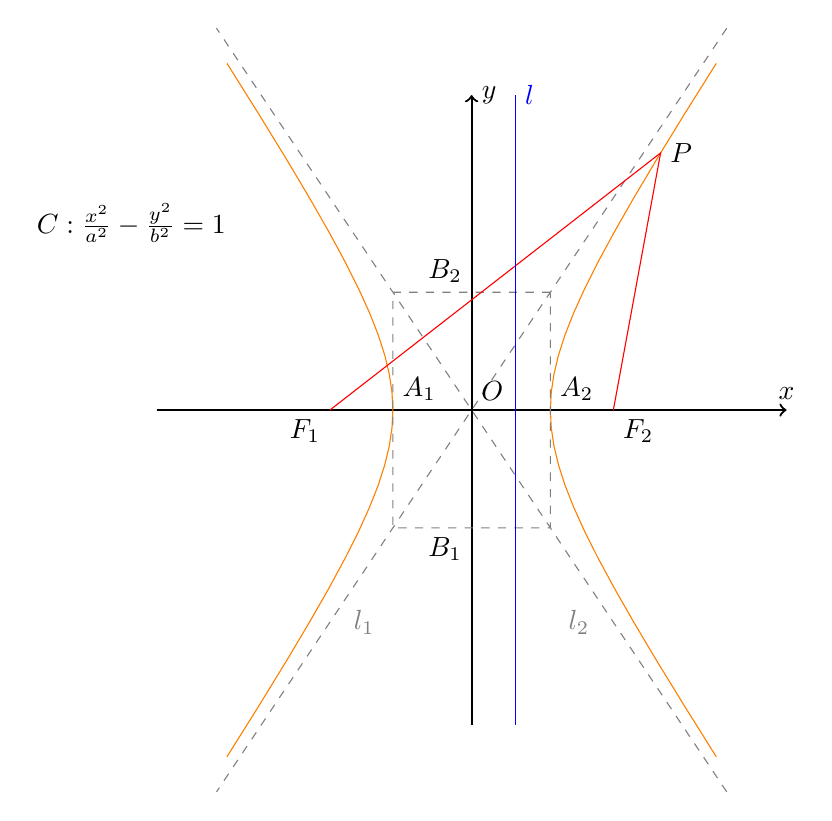
\begin{tikzpicture}
%\draw[gray,help lines,dashed] (-5,-3) grid (5,3);
\draw[thick,->] (-4,0) -- (4,0)node[above]{\(x\)};
\draw[thick,->] (0,-4) -- (0,4)node[right]{\(y\)};
\draw (-3,2)node[above left]{\(C: \frac{x^2}{a^2}-\frac{y^2}{b^2}=1\)};
\pgfmathsetmacro{\e}{1.8}   % eccentricity
\pgfmathsetmacro{\a}{1}
\pgfmathsetmacro{\b}{(\a*sqrt((\e)^2-1)}
\pgfmathsetmacro{\c}{(sqrt((\a)^2+(\b)^2))}
\pgfmathsetmacro{\px}{2.4}
\pgfmathsetmacro{\py}{sqrt(\b^2*(\px^2/\a^2-1))}
\pgfmathsetmacro{\d}{1.8} % 定义域
\draw[orange] plot[domain=-\d:\d] ({\a*cosh(\x)},{\b*sinh(\x)});
\draw[orange] plot[domain=-\d:\d] ({-\a*cosh(\x)},{\b*sinh(\x)});
\pgfmathsetmacro{\k}{1.8*\d}
\coordinate (F1) at (-\c,0);
\coordinate (F2) at (\c,0);
\coordinate (P) at (\px,\py);
\draw[gray,dashed] (\a,\b) -- (-\a,\b) -- (-\a,-\b) -- (\a,-\b) -- (\a,\b)
	(\k*\a,\k*\b) -- (-\k*\a,-\k*\b)
	(\k*\a,-\k*\b) -- (-\k*\a,\k*\b)
	(-\k*\a/2,-\k*\b/2)node[below right]{\(l_1\)}
	(\k*\a/2,-\k*\b/2)node[below left]{\(l_2\)};
\draw[red] (F1)node[below left,black]{\(F_1\)}
	-- (P)node[right,black]{\(P\)}
	-- (F2)node[below right,black]{\(F_2\)};
\pgfmathsetmacro{\dx}{\a^2/\c}
\draw[blue] (\dx,-4) -- (\dx,4)node[right]{\(l\)}; % 准线
\draw (0,0)node[above right]{\(O\)}
	(-\a,0)node[above right]{\(A_1\)}
	(\a,0)node[above right]{\(A_2\)}
	(0,-\b)node[below left]{\(B_1\)}
	(0,\b)node[above left]{\(B_2\)};
\end{tikzpicture}
\caption{双曲线的图形}
\label{figure:解析几何.双曲线的图形}
\end{figure}

我们根据双曲线的标准方程\[
\frac{x^2}{a^2} - \frac{y^2}{b^2} = 1
\]来研究它的几何性质.
\begin{enumerate}
\item 范围

由标准方程可知,双曲线上的点的坐标\((x,y)\)都适合不等式\(\frac{x^2}{a^2}\geq1\),即\(x^2 \geq a^2\),所以\(x \geq a\)或\(x \leq -a\).这说明双曲线在两条直线\(x = \pm a\)的外侧.

\item 对称性

双曲线关于每条坐标轴和原点都是对称的.这时,坐标轴是双曲线的对称轴,原点是双曲线的对称中心.双曲线的对称中心叫做双曲线的\DefineConcept{中心}.

\item 顶点

在标准方程中,令\(y=0\),得\(x = \pm a\),因此双曲线和\(x\)轴有两个交点\(A_1(-a,0)\)、\(A_2(a,0)\).因为\(x\)轴是双曲线的对称轴,所以双曲线和它的对称轴有两个焦点,它们叫做双曲线的\DefineConcept{顶点}.

令\(x=0\),得\(y^2=-b^2\),这个方程没有实数根,说明双曲线和\(y\)轴没有交点,但我们也把\(B_1(0,-b)\)和\(B_2(0,b)\)画在\(y\)轴上.

线段\(A_1 A_2\)叫做双曲线的\DefineConcept{实轴},它的长等于\(2a\),\(a\)叫做双曲线的实半轴长.
线段\(B_1 B_2\)叫做双曲线的\DefineConcept{虚轴},它的长等于\(2b\),\(b\)叫做双曲线的虚半轴长.

\item 渐近线

经过\(A_2\)、\(A_1\)作\(y\)轴的平行线\(x = \pm a\),经过\(B_2\)、\(B_1\)作\(x\)轴的平行线\(y = \pm b\),四条直线围成一个矩形.矩形的两条对角线所在的直线是\(y = \pm\frac{b}{a}x\).可以看出,双曲线的各支向外延伸时,与这两条直线逐渐接近.我们把这两条直线叫做双曲线的\DefineConcept{渐近线}.

在方程\(\frac{x^2}{a^2}-\frac{y^2}{b^2}=1\)中,如果\(a=b\),那么双曲线方程为\(x^2-y^2=a^2\),它的实轴和虚轴的长都等于\(2a\).这时,四条直线\(x=\pm a\)、\(y=\pm a\)围成正方形;渐近线方程成为\(x=\pm y\),它们互相垂直,并且平分双曲线实轴与虚轴所成的角.像这样,实轴和虚轴等长的双曲线叫做\DefineConcept{等轴双曲线}.

\item 离心率

双曲线的焦距与实轴的比\(e = \frac{c}{a}\),叫做双曲线的\DefineConcept{离心率}.因为\(c > a\),所以双曲线的离心率\(e > 1\).

由等式\(c^2-a^2=b^2\)可得\[
\frac{b}{a} = \frac{\sqrt{c^2-b^2}}{a} = \sqrt{\frac{c^2}{a^2}-1} = \sqrt{e^2-1}.
\]因此\(e\)越大,\(\frac{b}{a}\)也越大,即渐近线\(y = \pm\frac{b}{a}x\)的斜率的绝对值越大,这时双曲线的形状就从褊狭逐渐变得开阔.由此可知,双曲线的离心率越大,它的开口就越开阔.
\end{enumerate}

\begin{example}
以已知双曲线的虚轴为实轴,实轴为虚轴的双曲线叫做原双曲线的\DefineConcept{共轭双曲线}.求证:\begin{enumerate}
\item 双曲线和它的共轭双曲线有共同的渐近线;
\item 双曲线和它的共轭双曲线的四个焦点在同一个圆上.
\end{enumerate}
\begin{proof}
设已知双曲线的方程是\[
	\frac{x^2}{a^2}-\frac{y^2}{b^2}=1.
\]
它的焦点坐标为\(F_1(-c,0)\)和\(F_2(c,0)\)
(\(c^2=a^2+b^2\)).
它的渐近线方程是\(y=\pm\frac{b}{a}x\).

根据定义,其共轭双曲线的方程是\[
\frac{y^2}{a^2}-\frac{x^2}{b^2}=1.
\]它的交点坐标为\(F'_1(0,-c)\)和\(F'_2(0,c)\),
可见四个焦点都在圆\(x^2+y^2=c^2\)上.
它的共轭双曲线的渐近线方程是\(x=\pm\frac{a}{b}y\),
也即\(y=\pm\frac{b}{a}x\),
所以双曲线和它的共轭双曲线具有共同的渐近线.
\end{proof}
\end{example}

\begin{example}
点\(P(x,y)\)与定点\(F(c,0)\)的距离和它到定直线\(l: x = \frac{a^2}{c}\)的距离的比是常数\(\frac{c}{a}\)
(\(c > a > 0\)).
求点\(P\)的轨迹.
\begin{solution}
设点\(P\)到直线\(l\)的距离是\(d\),那么所求轨迹就是点集\[
\Set*{ P \given \frac{\abs{PF}}{d} = \frac{c}{a} },
\]由此得\[
\frac{\sqrt{(x-c)^2+y^2}}{\abs{\frac{a^2}{c}-x}} = \frac{c}{a},
\]化简得\[
(c^2-a^2)x^2 - a^2 y^2 = a^2(c^2-a^2).
\]设\(b^2=c^2-a^2\),则可将上式进一步化简为\[
\frac{x^2}{a^2}-\frac{y^2}{b^2}=1.
\]这是双曲线的标准方程,所以点\(P\)的轨迹是双曲线.
\end{solution}

由上例可知,点\(P\)与一个定点的距离和它到一条定直线的距离的比是常数
\(e = \frac{c}{a} > 1\)时,
这个点的轨迹是双曲线.
定点是双曲线的焦点,定直线叫做双曲线的\DefineConcept{准线},常数\(e\)是双曲线的离心率.

对于双曲线\(\frac{x^2}{a^2}-\frac{y^2}{b^2}=1\),相应于焦点\(F(c,0)\)的准线方程是\[
x = \frac{a^2}{c}
\quad\text{或}\quad
x = \frac{a}{e}.
\]根据双曲线的对称性,相应于焦点\(F'(-c,0)\)的准线方程是\(x=-\frac{a^2}{c}\),所以双曲线有两条准线.
\end{example}

\begin{example}
证明:等轴双曲线的离心率是\(\sqrt2\).
\begin{proof}
由定义,等轴双曲线\(x^2-y^2=a^2\)的实半轴长与虚半轴长相等,即\(a=b>0\),故\(c^2 = a^2 + b^2 = 2 a^2\),\(c = \sqrt2 a\),那么等轴双曲线的离心率为\[
e = \frac{c}{a} = \frac{\sqrt2 a}{a} = \sqrt2.
\qedhere
\]
\end{proof}
\end{example}

\begin{example}
证明:从双曲线的一个焦点到一条渐近线的距离等于虚半轴长.
\begin{proof}
设双曲线方程为\[
	\frac{x^2}{a^2}-\frac{y^2}{b^2}=1,
\]
它的右焦点为\(F(c,0)\)
(\(c^2=a^2+b^2\)),
其中一条渐近线为\(y=\frac{b}{a}x\)或\(bx-ay=0\).
由点到直线的距离公式,焦点\(F\)到上述渐近线的距离为\[
	d = \frac{\abs{b \cdot c - a \cdot 0}}{\sqrt{b^2+(-a)^2}}
	= \frac{bc}{c} = b.
	\qedhere
\]
\end{proof}
\end{example}

\begin{example}
已知双曲线\[
C: \frac{x^2}{a^2} - \frac{y^2}{b^2} = 1 \quad(a>b>1).
\]求双曲线在其上任意一点\(P_0(x_0,y_0)\)处的切线方程.
\begin{solution}
因为点\(P_0(x_0,y_0)\)在双曲线\(C\)上,所以\[
\frac{x_0^2}{a^2} - \frac{y_0^2}{b^2} = 1
\quad\text{即}\quad
b^2 x_0^2 - a^2 y_0^2 = a^2 b^2.
\]

当切线\(l\)与\(x\)轴相垂直时,显然只有\((-a,0)\)和\((a,0)\)两点可能是切点,
而它们各自的切线方程分别为\(x=-a\)和\(x=a\).

当切线\(l\)不与\(x\)轴相垂直时,
设切线方程为\(l: y = kx + p\),其中\(p = y_0 - k x_0\).
联立方程组,得\[
\begin{cases}
y = kx + p, \\
\frac{x^2}{a^2} - \frac{y^2}{b^2} = 1.
\end{cases}
\]那么有\[
\frac{1}{a^2} x^2 - \frac{1}{b^2} (kx+p)^2 = 1,
\]\[
b^2 x^2 - a^2 (k^2 x^2 + 2kpx + p^2) = a^2 b^2,
\]\[
(b^2 - a^2 k^2) x^2 - 2 a^2 k p x - a^2 (p^2 + b^2) = 0.
\]令判别式\(\Delta_1 = (2 a^2 k p)^2 + 4 (b^2 - a^2 k^2) a^2 (p^2 + b^2) = 0\),得\[
4 a^4 k^2 p^2 = 4 (a^2 k^2 - b^2) a^2 (p^2 + b^2),
\]\[
a^2 k^2 p^2 = (a^2 k^2 - b^2)(p^2 + b^2),
\]\[
a^2 b^2 k^2 = b^2(p^2 + b^2),
\]\[
a^2 k^2 = p^2 + b^2,
\]
代入\(p = y_0 - k x_0\),得\[
a^2 k^2 = (y_0 - k x_0)^2 + b^2,
\]\[
y_0^2 - 2k x_0 y_0 + k^2 x_0^2 + b^2 = a^2 k^2,
\]\[
(x_0^2 - a^2) k^2 - 2 x_0 y_0 k + (y_0^2 + b^2) = 0.
\]上式的判别式\(\Delta_2 = (2 x_0 y_0)^2 - 4(x_0^2 - a^2)(y_0^2 + b^2)
= 4(a^2 b^2 + a^2 y_0^2 - b^2 x_0^2) = 0\),故可解得\[
k = \frac{2 x_0 y_0}{2 (x_0^2 - a^2)}
= \frac{x_0 y_0}{x_0^2 - a^2}.
\]那么\(l\)的方程为\[
y - y_0 = \frac{x_0 y_0}{x_0^2 - a^2} (x - x_0),
\]\[
(x_0^2 - a^2) y = x_0 y_0 x + (x_0^2 - a^2) y_0 - x_0^2 y_0
= x_0 y_0 x - a^2 y_0,
\]\[
x_0 y_0 x + (a^2 - x_0^2) y = a^2 y_0,
\]\[
\frac{x_0 x}{a^2} + (a^2 - x_0^2) \frac{y_0 y}{a^2 y_0^2} = 1,
\]\[
\frac{x_0 x}{a^2} + (a^2 - x_0^2) \frac{y_0 y}{(x_0^2 - a^2) b^2} = 1,
\]最后化简得\begin{equation}\label{equation:解析几何.双曲线的切线}
\frac{x_0 x}{a^2} - \frac{y_0 y}{b^2} = 1.
\end{equation}
这就是双曲线在其上任意一点\(P_0(x_0,y_0)\)处的切线方程.
\end{solution}
\end{example}

\begin{theorem}[双曲线的焦点三角形]
设\(P\)是双曲线\(C: \frac{x^2}{a^2} - \frac{y^2}{b^2} = 1\ (a>0,b>0)\)上任一点,
\(F_1\)、\(F_2\)是\(C\)的焦点,那么\[
S_{\triangle P F_1 F_2} = \frac{b^2}{\tan(\theta/2)},
\]其中\(\theta=\angle{F_1 P F_2}\).
\end{theorem}

\subsection{抛物线}
\begin{definition}
在平面内,与一个定点和一条定直线的距离相等的点的集合,
叫做\DefineConcept{抛物线}(parabola).
这个定点叫做抛物线的\DefineConcept{焦点}.
这条定直线叫做抛物线的\DefineConcept{准线}.
\end{definition}

取经过焦点\(F\)且垂直于准线\(l\)的直线为\(x\)轴,\(x\)轴于\(l\)相交于点\(K\),以线段\(KF\)的垂直平分线为\(y\)轴.设\(\abs{KF}=p\),
那么,焦点\(F\)的坐标为\((\frac{p}{2},0)\),准线\(l\)的方程为\(x=-\frac{p}{2}\).

设抛物线上的点\(P(x,y)\)到\(l\)的距离为\(d\).抛物线就是点集\[
\Set*{ P \given \abs{PF} = d }.
\]因为\(\abs{PF} = \sqrt{\left(x-\frac{p}{2}\right)^2+y^2}\),\(d = \abs{x+\frac{p}{2}}\),所以\[
\sqrt{\left(x-\frac{p}{2}\right)^2+y^2} = \abs{x+\frac{p}{2}}.
\]将上式两边平方,并化简得\begin{equation}
y^2 = 2px, \quad p > 0.
\end{equation}
这个方程叫做\DefineConcept{抛物线的标准方程},它所表示的抛物线的焦点在\(x\)轴的正半轴上,
坐标是\((\frac{p}{2},0)\),准线方程是\(x=-\frac{p}{2}\).

一条抛物线,由于它在坐标平面上的位置不同,方程也不同,所以抛物线的标准方程还有其他几种形式:\(y^2 = -2px\)、\(x^2 = 2py\)、\(x^2 = -2py\).

\begin{figure}[ht]
\centering
\begin{tikzpicture}
%\draw[gray,help lines,dashed] (-3,-3) grid (3,3);
\draw[thick,->] (-3,0) -> (4,0)node[above]{\(x\)};
\draw[thick,->] (0,-4) -> (0,4)node[right]{\(y\)};
\draw (0,0)node[below left]{\(O\)};
\pgfmathsetmacro{\p}{2}
\pgfmathsetmacro{\x}{3}
\pgfmathsetmacro{\y}{sqrt(2*\p*\x)}
\pgfmathsetmacro{\f}{\p/2}
\coordinate (F)at(\f,0);
\draw[orange] [rotate=-90](0,0)parabola(\y,\x) [rotate=180](0,0)parabola(\y,-\x);
\draw[purple] (-\f,-4)--(-\f,4);
\draw (2,2)node[above right]{\(C: y^2 = 2px\ (p>0)\)}
	(-\f,-1)node[below left]{\(l: x = -\frac{p}{2}\)};
\fill (F)circle(2pt)node[below right]{\(F\)};
\pgfmathsetmacro{\px}{\f/2}
\pgfmathsetmacro{\py}{\p/sqrt(2)}
\coordinate (P)at(\px,\py);
\coordinate (Q)at(-\f,\py);
\coordinate (K)at(-\f,0);
\draw[red] (F)--(P)node[above,black]{\(P\)}--(Q)node[left,black]{\(Q\)}
	pic[draw=gray,-,angle radius=0.3cm]{right angle=P--Q--K};
\draw (K)node[below left]{\(K\)};
\coordinate (M)at(\f,\p);
\coordinate (N)at(\f,-\p);
\draw[blue] (M)node[above,black]{\(M\)}--(N)node[below,black]{\(N\)}
	pic[draw=gray,-,angle radius=0.3cm]{right angle=N--F--K};
\end{tikzpicture}
\caption{抛物线的图形}
\label{figure:解析几何.抛物线的图形}
\end{figure}

我们根据抛物线的标准方程\[
y^2 = 2px, \quad p > 0
\]来研究它的几何性质.
\begin{enumerate}
\item 范围

因为\(p>0\),由标准方程可知,抛物线上的点的坐标\((x,y)\)都适合不等式\(x \geq 0\),所以这条抛物线在\(y\)轴的右侧.当\(x\)的值增大时,\(\abs{y}\)也增大,这说明抛物线向右上方和右下方无限延伸.

\item 对称性

以\(-y\)代\(y\),标准方程形式不变,所以这个抛物线关于\(x\)轴对称,我们把抛物线的对称轴叫做抛物线的\DefineConcept{轴}.

\item 顶点

抛物线和它的轴的交点叫做抛物线的\DefineConcept{顶点}.
在标准方程中,当\(y=0\)时,\(x=0\),因此标准方程所表示的抛物线的顶点就是坐标原点.

\item 离心率

抛物线上的点\(P\)与焦点和准线的距离的比,叫做抛物线的\DefineConcept{离心率},用\(e\)表示.
由抛物线的定义,抛物线的离心率为\(e = 1\).
\end{enumerate}

\begin{example}
已知抛物线方程\(C: y^2=2px\ (p>0)\).
下面讨论过焦点\(F(p/2,0)\)的直线\(l\)与抛物线的交点个数.
\begin{enumerate}
	\item 当直线\(l\)的方程为\(y=0\)时,
	代入抛物线方程得\(2px = 0\),解得\(x=0\).
	可见直线\(l\)与抛物线\(C\)只有一个交点,即坐标原点\(O\).

	\item 当直线\(l\)的方程为\(x=p/2\)时,
	代入抛物线方程得\(y^2=2p\cdot(p/2)=p^2\),解得\(y=\pm p\).
	可见直线\(l\)与抛物线\(C\)有两个交点\(P(p/2,p)\)和\(Q(p/2,-p)\).
	焦点弦长为\(\abs{PQ} = 2p\).

	\begin{center}
		\begin{tikzpicture}
			%\draw[gray,help lines,dashed] (-3,-3) grid (3,3);
			\draw[thick,->] (-2,0) -> (4,0)node[above]{\(x\)};
			\draw[thick,->] (0,-4) -> (0,4)node[right]{\(y\)};
			\draw (0,0)node[below left]{\(O\)};
			\pgfmathsetmacro{\p}{2}  % 参数p
			\pgfmathsetmacro{\x}{3}
			\pgfmathsetmacro{\y}{sqrt(2*\p*\x)}
			\pgfmathsetmacro{\f}{\p/2}  % 焦点横坐标
			\coordinate (F)at(\f,0);
			\coordinate (2F)at(2\f,0);
			\draw[orange] [rotate=-90](0,0)parabola(\y,\x) [rotate=180](0,0)parabola(\y,-\x);
			\draw[purple] (-\f,-4)--(-\f,4); % 准线
			\draw (2,-3)node[above right]{\(C: y^2 = 2px\ (p>0)\)};
			\pgfmathsetmacro{\k}{3}  % 焦点弦 斜率
			\pgfmathsetmacro{\a}{\p/(2*\k^2)}
			\pgfmathsetmacro{\b}{\p/\k}
			\pgfmathsetmacro{\c}{sqrt(\k^2+1)}
			\pgfmathsetmacro{\px}{\a*(\c+1)^2}
			\pgfmathsetmacro{\py}{\b*(\c+1)}
			\pgfmathsetmacro{\qx}{\a*(\c-1)^2}
			\pgfmathsetmacro{\qy}{-\b*(\c-1)}
			\coordinate (P)at(\px,\py);
			\coordinate (Q)at(\qx,\qy);
			\coordinate (P1)at(-\f,\py);
			\coordinate (Q1)at(-\f,\qy);
			\coordinate (K)at(-\f,0);
			\fill (P)circle(2pt)node[below right]{\(P\)}
				(F)circle(2pt)node[below right]{\(F\)}
				(Q)circle(2pt)node[right]{\(Q\)};
			\draw[red] (P)--(P1)node[left,black]{\(P_1\)}
				pic[draw=gray,-,angle radius=0.3cm]{right angle=P--P1--K}
				(Q)--(Q1)node[left,black]{\(Q_1\)}
				pic[draw=gray,-,angle radius=0.3cm]{right angle=Q--Q1--K};
			\draw[blue] (P)--(F)--(Q);
			\draw pic["\(\theta\)",draw=gray,-,angle eccentricity=1.7,angle radius=5mm]{angle=2F--F--P};
		\end{tikzpicture}
	\end{center}

	\item 当直线\(l\)的方程为\(y=k\left(x-\frac{p}{2}\right)\ (k\neq0)\)时,代入抛物线方程得\[
		\left[k \left(x-\frac{p}{2}\right)\right]^2 = 2px,
	\]
	化简得\begin{gather}
		k^2 x^2 - (k^2 + 2)px + \frac{1}{4} k^2 p^2 = 0, \tag1
	\end{gather}
	因为\[
		\Delta = [- (k^2 + 2)p]^2 - 4 k^2 \frac{1}{4} k^2 p^2
		= 4 p^2 (k^2 + 1) > 0,
	\]
	所以(1)式总有两个实根\[
		x_{1,2} = \frac{(k^2+2)p \pm \sqrt\Delta}{2 k^2}
		= \frac{p}{2 k^2} (\sqrt{k^2+1} \pm 1)^2.
	\]
	可见直线\(l\)与抛物线\(C\)有两个交点\(P(x_1,y_1)\)和\(Q(x_2,y_2)\).
	不妨设\(x_1 > x_2\),即\[
		x_1 = \frac{(k^2+2)p + \sqrt\Delta}{2 k^2}
		= \frac{p}{2 k^2} (\sqrt{k^2+1} + 1)^2,
	\]\[
		x_2 = \frac{(k^2+2)p - \sqrt\Delta}{2 k^2}
		= \frac{p}{2 k^2} (\sqrt{k^2+1} - 1)^2.
	\]
	将\(x_{1,2}\)代入抛物线方程得\[
		y^2 = 2 p^2 \frac{(\sqrt{k^2+1}\pm1)^2}{2 k^2}
		= \frac{p^2}{k^2} (\sqrt{k^2+1}\pm1)^2,
	\]\[
		y = \pm \frac{p}{k} (\sqrt{k^2+1}\pm1).
	\]
	当\(k>0\)时,由\(x_1 > x_2\)可知\(y_1 > 0 > y_2\),那么\[
		y_1 = \frac{p}{k} (\sqrt{k^2+1}+1),
		\qquad
		y_2 = -\frac{p}{k} (\sqrt{k^2+1}-1).
	\]
	由两点间距离公式,焦点弦长为\begin{equation}
		\abs{PQ} = \sqrt{
		\left(\frac{p}{2 k^2} \cdot 4 \sqrt{k^2+1}\right)^2
		+\left(\frac{p}{k} \cdot 2 \sqrt{k^2+1}\right)^2
		} = 2p \left(1+\frac{1}{k^2}\right).
	\end{equation}
	若记\(k=\tan\theta\),则上述弦长公式也可改写为\begin{equation}
		\abs{PQ} = 2p \frac{\tan^2\theta+1}{\tan^2\theta}
		= 2p \frac{\sec^2\theta}{\tan^2\theta}
		= 2p \frac{1}{\sin^2\theta}
		= 2p \csc^2\theta.
	\end{equation}

	现在我们来检验上述弦长公式的正确性.
	根据抛物线的定义,抛物线上一点到焦点与其到准线的距离相等,
	故\(\abs{PF} = \abs{P P_1} = x_1 + \frac{p}{2}\),
	\(\abs{QF} = \abs{Q Q_1} = x_2 + \frac{p}{2}\),
	那么\(\abs{PQ} = \abs{PF}+\abs{QF} = x_1 + x_2 + p\).
	代入\(x_{1,2}\),得\begin{align*}
		\abs{PQ} &= \frac{p}{2 k^2} \left[(\sqrt{k^2+1} + 1)^2 + (\sqrt{k^2+1} - 1)^2\right] + p \\
		&= p\left[\frac{2(k^2 + 1) + 2}{2 k^2} + 1\right]
		= p \frac{4k^2 + 4}{2k^2}
		= 2p \left(1+\frac{1}{k^2}\right).
	\end{align*}
\end{enumerate}

另外,可以注意到,\(P\)、\(Q\)两点的坐标满足\begin{equation}
	x_1 \cdot x_2 = \frac{p^2}{4},
	\qquad
	y_1 \cdot y_2 = -p^2.
\end{equation}

\(P\)、\(Q\)两点的焦半径\(\abs{FP}\)、\(\abs{FQ}\)满足\begin{equation}
	\frac{1}{\abs{FP}} + \frac{1}{\abs{FB}}
	= \frac{2}{p}.
\end{equation}
\end{example}


\section{常见曲面}
本章将介绍一些常见曲面,
一方面了解如何利用曲面的几何特性建立它的方程,
另一方面熟悉如何利用方程研究曲面的几何性质.

\subsection{球面和旋转面}
\subsubsection{球面的一般方程}
我们来求球心为\(M_0(x_0,y_0,z_0)\),半径为\(R\)的球面的方程.
点\(M(x,y,z)\)在这个球面上的充分必要条件是\(\abs{\vec{M_0 M}} = R\),即
\begin{equation}\label{equation:解析几何.球面的标准方程}
	(x-x_0)^2+(y-y_0)^2+(z-z_0)^2=R^2,
\end{equation}
展开得
\begin{equation}\label{equation:解析几何.球面的一般方程}
	x^2 + y^2 + z^2 + 2 b_1 x + 2 b_2 y + 2 b_3 z + c = 0,
\end{equation}
其中\(b_1 = -x_0\),
\(b_2 = -y_0\),
\(b_3 = -z_0\),
\(c = x_0^2 + y_0^2 + z_0^2 - R^2\).

\cref{equation:解析几何.球面的标准方程}
和\cref{equation:解析几何.球面的一般方程}
就是所求球面的方程,
它是一个三元二次方程,
没有交叉项(即含\(xy,xz,yz\)的项),
平方项的系数相同.
反之,任一形如\cref{equation:解析几何.球面的一般方程} 的方程也可经过配方得到
\begin{equation}\label{equation:解析几何.形如球面的一般方程的方程经过配方所得方程}
	(x+b_1)^2 + (y+b_2)^2 + (z+b_3)^2 + (c-b_1^2-b_2^2-b_3^2) = 0.
\end{equation}
当\(b_1^2+b_2^2+b_3^2>c\)时,
\cref{equation:解析几何.形如球面的一般方程的方程经过配方所得方程}
表示一个球心在\((-b_1,-b_2,-b_3)\),半径为\(\sqrt{b_1^2+b_2^2+b_3^2-c}\)的球面;
当\(b_1^2+b_2^2+b_3^2=c\)时,
它表示一个点\((-b_1,-b_2,-b_3)\);
当\(b_1^2+b_2^2+b_3^2<c\)时,
它没有轨迹(或者说它表示一个虚球面).

\subsubsection{球面的参数方程,点的球面坐标}
如果球心在原点,半径为\(R\),在球面上任取一点\(M(x,y,z)\),
从\(M\)作\(Oxy\)平面的垂线,垂足为\(N\),
连接\(OM,ON\),
设\(x\)轴的正半轴到\(\vec{ON}\)的角度为\(\phi\),
\(\vec{ON}\)到\(\vec{OM}\)的角度为\(\theta\)
(\(M\)在\(Oxy\)平面上方时,\(\theta>0\);否则\(\theta<0\)),
则有
\begin{equation}\label{equation:解析几何.球心在原点半径为R的球面的参数方程}
	\left\{ \begin{array}{l}
		x = R \cos\theta \cos\phi, \\
		y = R \cos\theta \sin\phi, \\
		z = R \sin\theta,
	\end{array} \right.
	\quad
	-\frac{\pi}{2} \leq \theta \leq \frac{\pi}{2},
	-\pi < \phi \leq \pi.
\end{equation}
\cref{equation:解析几何.球心在原点半径为R的球面的参数方程}
称为“球心在原点、半径为R的球面的\DefineConcept{参数方程}”;
它有两个参数\(\theta,\phi\),
其中\(\theta\)称为\DefineConcept{纬度},
\(\phi\)称为\DefineConcept{经度}.
球面上的每一个点(除去它与\(z\)轴的交点)对应唯一的实数对\((\theta,\phi)\),
因此\((\theta,\phi)\)称为“球面上的点的\DefineConcept{曲纹坐标}”.

因为几何空间中任一点\(M(x,y,z)\)必在以原点为球心,yi
以\(R=\abs{\vec{OM}}\)为半径的球面上,
而球面上的点(除去它与\(z\)轴的交点外)
又由它的曲纹坐标\((\theta,\phi)\)唯一确定,
因此,除去\(z\)轴外,几何空间中的点\(M\)由有序三元实数组\((R,\theta,\phi)\)唯一确定.
我们把\((R,\theta,\phi)\)称为“几何空间中的点的\DefineConcept{球面坐标}或\DefineConcept{空间极坐标}”,
其中\[
	R \geq 0,
	\qquad
	-\frac{\pi}{2} \leq \theta \leq \frac{\pi}{2},
	\qquad
	-\pi < \phi \leq \pi.
\]

\subsubsection{曲面和曲线的一般方程、参数方程}
从球面的方程 \labelcref{equation:解析几何.球面的一般方程}
和球面的参数方程 \labelcref{equation:解析几何.球心在原点半径为R的球面的参数方程} 看到,
一般来说,曲面的一般方程是一个三元方程
\begin{equation}\label{equation:解析几何.曲面的一般方程}
	F(x,y,z) = 0,
\end{equation}
曲面的参数方程是含两个参数的方程
\begin{equation}\label{equation:解析几何.曲面的参数方程}
	\left\{ \begin{array}{l}
		x = x(u,v), \\
		y = y(u,v), \\
		z = z(u,v),
	\end{array} \right.
	\quad
	a \leq u \leq b,
	c \leq v \leq d.
\end{equation}
对于\((u,v)\)的每一对值,
由方程 \labelcref{equation:解析几何.曲面的参数方程} 确定的点\((x,y,z)\)都在此曲面上;
而此曲面上任一点的坐标都可由\((u,v)\)的某一对值
通过方程 \labelcref{equation:解析几何.曲面的参数方程} 表示.
于是,通过曲面的参数方程 \labelcref{equation:解析几何.曲面的参数方程},
曲面上的点(可能要除去个别点)便可由数对\((u,v)\)来确定,
于是称\((u,v)\)为“曲面上的点的\DefineConcept{曲纹坐标}”.

我们可以给出如下定义.
\begin{definition}
如果曲面\(S\)与三元方程\[
	F(x,y,z)=0
\]满足
\begin{enumerate}
	\item 曲面\(S\)上任一点的坐标都满足这个三元方程,
	\item 不在曲面\(S\)上的点的坐标都不满足这个三元方程,
\end{enumerate}
那么,方程\(F(x,y,z)=0\)就叫做“曲面\(S\)的\DefineConcept{方程}”,
而曲面\(S\)就叫做“方程\(F(x,y,z)=0\)的\DefineConcept{图形}”.
\end{definition}

由于几何空间中曲线可以看成两个曲面的交线,
所以它的一般方程就是联立两个三元方程所得的方程组\begin{equation}\label{equation:解析几何.曲线的一般方程}
	\left\{ \begin{array}{l}
		F(x,y,z) = 0, \\
		G(x,y,z) = 0;
	\end{array} \right.
\end{equation}
而它的参数方程则是含有一个参数的方程
\begin{equation}\label{equation:解析几何.曲线的参数方程}
	\left\{ \begin{array}{l}
		x = x(t), \\
		y = y(t), \\
		z = z(t),
	\end{array} \right.
	\quad
	a \leq t \leq b.
\end{equation}
对于\(t\)的每一个值,
由方程 \labelcref{equation:解析几何.曲线的参数方程} 确定的点\((x,y,z)\)都在此曲线上;
而此曲线上任一点的坐标都可由\(t\)的某个值
通过方程 \labelcref{equation:解析几何.曲线的参数方程} 表示.

\subsubsection{旋转面}
球面可以看成一个半圆绕它的直径旋转一周所形成的曲面.
现在来研究更一般的情形.

我们称一条曲线\(\Gamma\)绕一条直线\(l\)旋转所得的曲面为\DefineConcept{旋转面},
其中\(l\)称为\DefineConcept{轴},\(\Gamma\)称为\DefineConcept{母线}.

母线\(\Gamma\)上的任一点\(M_0\)绕\(l\)旋转会得到一个圆,我们称之为\DefineConcept{纬圆}.
纬圆所在的平面与轴\(l\)垂直.
过\(l\)的半平面与旋转面的交线称为\DefineConcept{经线}.
经线可以作为母线,但母线不一定是经线.

已知轴\(l\)经过点\(M_1(x_1,y_1,z_1)\),
方向向量为\(\vb{\nu}=(A,B,C)\),
母线\(\Gamma\)的方程为\[
	\left\{ \begin{array}{l}
		F(x,y,z) = 0, \\
		G(x,y,z) = 0.
	\end{array} \right.
\]
点\(M(x,y,z)\)在旋转面上的充分必要条件是
\(M\)在经过母线\(\Gamma\)上某一点\(M_0(x_0,y_0,z_0)\)的纬圆上,
即有母线\(\Gamma\)上的一点\(M_0\),
使得\(M\)和\(M_0\)到轴\(l\)的距离相等
(或到轴上一点\(M_1\)的距离相等),
并且\(\vec{M_0 M} \perp l\).
因此有\[
	\left\{ \begin{array}{l}
		F(x_0,y_0,z_0) = 0, \\
		G(x_0,y_0,z_0) = 0, \\
		\abs{\vec{M M_1} \times \vb{\nu}} = \abs{\vec{M_0 M_1} \times \vb{\nu}}, \\
		A(x-x_0) + B(y-y_0) + C(z-z_0) = 0.
	\end{array} \right.
\]
从这个方程组中消去参数\(x_0,y_0,z_0\),就得到关于\(x,y,z\)的方程,它就是所求旋转面的方程.

现在设旋转面的轴是\(z\)轴,
母线\(\Gamma\)在\(Oyz\)平面上,
其方程为\[
	\left\{ \begin{array}{l}
		f(y,z) = 0, \\
		x = 0,
	\end{array} \right.
\]
则点\(M(x,y,z)\)在旋转面上的充分必要条件是\[
	\left\{ \begin{array}{l}
		f(y_0,z_0) = 0, \\
		x_0 = 0, \\
		x^2+y^2=x_0^2+y_0^2, \\
		1\cdot(z-z_0) = 0.
	\end{array} \right.
\]
消去参数\(x_0,y_0,z_0\),得
\begin{equation}\label{equation:解析几何.Oyz平面上的曲线绕z轴旋转所得旋转面的方程}
	f(\pm\sqrt{x^2+y^2},z) = 0.
\end{equation}
\cref{equation:解析几何.Oyz平面上的曲线绕z轴旋转所得旋转面的方程} 就是所求旋转面的方程.
由此可见,为了得到由\(Oyz\)平面上的曲线\(\Gamma\)绕\(z\)轴旋转所得旋转面的方程,
只要将母线\(\Gamma\)在\(Oyz\)平面上的方程中的\(y\)改为\(\pm\sqrt{x^2+y^2}\),保持\(z\)不变.
坐标平面上的曲线绕坐标轴旋转所得旋转面的方程都有类似的规律.

\begin{table}[ht]
	\centering
	\begin{tabular}{|c|c|c|}
	\hline
	曲线方程 & 旋转轴 & 旋转曲面方程 \\ \hline
	\multirow{2}{*}{\(f(x,y)=0\)} & \(x\) & \(f(x,\pm\sqrt{y^2+z^2})=0\) \\ \cline{2-3}
		& \(y\) & \(f(\pm\sqrt{x^2+z^2},y)=0\) \\ \hline
	\multirow{2}{*}{\(f(y,z)=0\)} & \(y\) & \(f(y,\pm\sqrt{x^2+z^2})=0\) \\ \cline{2-3}
		& \(z\) & \(f(\pm\sqrt{x^2+y^2},z)=0\) \\ \hline
	\multirow{2}{*}{\(f(x,z)=0\)} & \(x\) & \(f(x,\pm\sqrt{y^2+z^2})=0\) \\ \cline{2-3}
		& \(z\) & \(f(\pm\sqrt{x^2+y^2},z)=0\) \\
	\hline
	\end{tabular}
	\caption{}
\end{table}


\begin{example}
母线\[
	\Gamma: \left\{ \begin{array}{l}
		y^2 = 2pz, \\
		x = 0,
	\end{array} \right.
	\quad p>0
\]
绕\(z\)轴旋转所得旋转面的方程为\[
	x^2+y^2=2pz.
\]
这个曲面称为\DefineConcept{旋转抛物面}.
\end{example}

\begin{example}
母线\[
	\Gamma: \left\{ \begin{array}{l}
		\frac{x^2}{a^2}-\frac{y^2}{b^2}=1, \\
		z=0
	\end{array} \right.
\]
绕\(x\)旋转所得旋转面的方程为\[
	\frac{x^2}{a^2}-\frac{y^2+z^2}{b^2}=1.
\]
这个曲面称为\DefineConcept{旋转双叶双曲面}.

母线\(\Gamma\)绕\(y\)轴旋转所得旋转面的方程为\[
	\frac{x^2+z^2}{a^2}-\frac{y^2}{b^2}=1.
\]
这个曲面称为\DefineConcept{旋转单叶双曲面}.
\end{example}

\begin{example}
圆\[
	\left\{ \begin{array}{l}
		(x-a)^2+z^2=r^2, \\
		y=0,
	\end{array} \right.
	\quad 0<r<a
\]
绕\(z\)轴旋转所得旋转面的方程为\[
	(\pm\sqrt{x^2+y^2}-a)^2+z^2=r^2,
\]
即\[
	(x^2+y^2+z^2+a^2-r^2)^2=4a^2(x^2+y^2).
\]
这个曲面称为\DefineConcept{环面}.
\end{example}

\subsection{柱面和锥面}
\subsubsection{柱面方程的建立}
一条直线\(l\)沿着一条空间曲线\(C\)平行移动时所形成的曲面称为\DefineConcept{柱面},
其中\(l\)称为\DefineConcept{母线},\(C\)称为\DefineConcept{准线}.

由于平面可以看成是由一条直线沿着另一条与之相交的直线平行移动所形成的,故平面也是柱面.

对于任意一个柱面,它的准线和母线都不唯一.
但是,除去平面以外,任意柱面的母线方向是唯一的.
与每一条母线都相交的曲线均可作为准线.

设一个柱面的母线方向为\(\vb{\nu}=(A,B,C)\),
准线的方程为\[
	\left\{ \begin{array}{l}
		F(x,y,z) = 0, \\
		G(x,y,z) = 0.
	\end{array} \right.
\]
我们来求这个柱面的方程.

点\(M(x,y,z)\)在此柱面上的充分必要条件是\(M\)在某一条母线上,
即有准线\(C\)上一点\(M_0(x_0,y_0,z_0)\),
使得\(M\)在经过\(M_0\)且方向向量为\(\vb{\nu}\)的直线上.
因此有\[
	\left\{ \begin{array}{l}
		F(x_0,y_0,z_0) = 0, \\
		G(x_0,y_0,z_0) = 0, \\
		x = x_0 + Au, \\
		y = y_0 + Bu, \\
		z = z_0 + Cu.
	\end{array} \right.
\]
消去\(x_0,y_0,z_0\),得\[
	\left\{ \begin{array}{l}
		F(x - Au,y - Bu,z - Cu) = 0, \\
		G(x - Au,y - Bu,z - Cu) = 0.
	\end{array} \right.
\]
再消去参数\(u\),得到关于\(x,y,z\)的一个方程,
它就是所求柱面的方程.

如果给定的准线\(C\)的方程是一个参数方程\[
	\left\{ \begin{array}{l}
		x = f(t), \\
		y = g(t), \\
		z = h(t),
	\end{array} \right.
	\quad a \leq t \leq b,
\]
则同理可得柱面的参数方程为\[
	\left\{ \begin{array}{l}
		x = f(t) + Au, \\
		y = g(t) + Bu, \\
		z = h(t) + Cu,
	\end{array} \right.
	\quad
	a \leq t \leq b,
	-\infty < u < +\infty.
\]

\subsubsection{圆柱面,点的柱面坐标}
现在来看圆柱面的方程.
圆柱面有一条对称轴\(l\),
圆柱面上每一个点到轴\(l\)的距离都相等,
这个距离称为圆柱面的半径.
圆柱面的准线可取成一个圆\(C\),
它的母线方向与准线圆垂直.
如果知道准线圆的方程和母线方向,
则可用前一目中所述的方法求出圆柱面的方程.
如果知道圆柱面的半径为\(r\),母线方向为\(\vb{\nu}=(A,B,C)\),
以及圆柱面的对称轴\(l\)经过点\(M_0(x,y,z)\),
则点\(M(x,y,z)\)在此圆柱面上充分必要条件是\(M\)到轴\(l\)的距离等于\(r\),即\[
	\frac{\abs{\vec{M M_0} \times \vb{\nu}}}{\abs{\vb{\nu}}} = r.
\]
由此出发可求得圆柱面的方程.
特别地,设圆柱面的对称轴为\(z\)轴,
则这个圆柱面的方程为
\begin{equation}\label{equation:解析几何.以z轴为对称轴r为半径的圆柱面的一般方程}
	x^2+y^2=r^2.
\end{equation}

由于几何空间中任意一点\(M(x,y)\)
必在以\(r=\sqrt{x^2+y^2}\)为半径,
\(z\)轴为对称轴的圆柱面上,xi
显然这个圆柱面的参数方程为\[
	\left\{ \begin{array}{l}
		x = r \cos\theta, \\
		y = r \sin\theta, \\
		z = u,
	\end{array} \right.
	\quad 0\leq \theta < 2\pi,
	-\infty < u < +\infty.
\]
因此,圆柱面上的点\(M\)可以由数对\((\theta,u)\)所确定,
从而几何空间中任意一点\(M\)被有序三元实数组\((r,\theta,u)\)所确定.
\((r,\theta,u)\)称为点\(M\)的\DefineConcept{柱面坐标}.

\subsubsection{柱面方程的特点}
从\cref{equation:解析几何.以z轴为对称轴r为半径的圆柱面的一般方程} 看到,
母线平行于\(z\)轴的圆柱面的方程中不含\(z\),或者说\(z\)的系数为零.
这个结论对于一般的柱面也成立.
\begin{theorem}
%@see: 《解析几何》(丘维声) P86 定理2.1
若一个柱面的母线平行于\(x\)轴,则它的方程中不含\(x\);
若它的母线平行于\(y\)轴,则它的方程中不含\(y\);
若它的母线平行于\(z\)轴,则它的方程中不含\(z\).
反之,若一个三元方程不含\(x\),则它一定表示一个母线平行于\(x\)轴的柱面;
若这个方程不含\(y\),则它一定表示一个母线平行于\(y\)轴的柱面;
若这个方程不含\(z\),则它一定表示一个母线平行于\(z\)轴的柱面.
\begin{proof}
设一个柱面的母线平行于\(z\)轴,则这个柱面的每条母线必与\(Oxy\)平面相交,
从而这个柱面与\(Oxy\)平面的交线\(C\)可以作为准线.
设\(C\)的方程是\[
	\left\{ \begin{array}{l}
		f(x,y) = 0, \\
		z = 0.
	\end{array} \right.
\]
点\(M\)在此柱面上的充分必要条件是:
存在准线\(C\)上一点\(M_0(x_0,y_0,z_0)\),
使得\(M\)在经过\(M_0\)且方向向量为\(\vb{\nu}=(0,0,1)\)的直线上.
因此有\[
	\left\{ \begin{array}{l}
		f(x_0,y_0) = 0, \\
		z_0 = 0, \\
		x = x_0, \\
		y = y_0, \\
		z = z_0 + u.
	\end{array} \right.
\]
消去\(x_0,y_0,z_0\),得\[
	\left\{ \begin{array}{l}
		f(x,y) = 0, \\
		z = u.
	\end{array} \right.
\]
由于参数可以取任意实数值,于是得到这个柱面的方程为\[
	f(x,y) = 0.
\]

反之,任给一个不含\(z\)的三元方程\(g(x,y)=0\),我们考虑以曲线\[
	D: \left\{ \begin{array}{l}
		g(x,y) = 0, \\
		z = 0
	\end{array} \right.
\]
为准线,\(z\)轴方向为母线方向的柱面.
由上述讨论可知,这个柱面的方程为\(g(x,y)=0\).
因此,方程\(g(x,y)=0\)表示一个母线平行于\(z\)轴的柱面.

母线平行于\(x\)轴和\(y\)轴的情形可以类似讨论.
\end{proof}
\end{theorem}

\begin{example}
方程\[
	\frac{x^2}{a^2} + \frac{y^2}{b^2} - 1 = 0
\]
表示母线平行于\(z\)轴的柱面,它与\(Oxy\)平面的交线为\[
	\left\{ \begin{array}{l}
		\frac{x^2}{a^2} + \frac{y^2}{b^2} = 1, \\
		z = 0.
	\end{array} \right.
\]
这条交线是椭圆,因而这个柱面称为\DefineConcept{椭圆柱面}.

类似地,方程\[
	\frac{x^2}{a^2} - \frac{y^2}{b^2} + 1 = 0
\]
表示母线平行于\(z\)轴的双曲柱面;
方程\[
	x^2 + 2py = 0
	\quad(p>0)
\]
表示母线平行于\(z\)轴的抛物柱面.
\end{example}

\subsubsection{锥面方程的建立}
在几何空间中,由曲线\(C\)上的点
与不在\(C\)上的一个定点\(M_0\)的连线组成的曲面称为\DefineConcept{锥面},
其中\(M_0\)称为\DefineConcept{顶点},\(C\)称为\DefineConcept{准线},
\(C\)上的点与\(M_0\)的连线称为\DefineConcept{母线}.

一个锥面的准线不唯一,锥面上与每一条母线都相交的曲线均可作为准线.

设一个锥面的顶点为\(M_0(x_0,y_0,z_0)\),准线\(C\)的方程为\[
	\left\{ \begin{array}{l}
		F(x,y,z) = 0, \\
		G(x,y,z) = 0.
	\end{array} \right.
\]
我们来求这个锥面的方程.

点\(M(x,y,z)\neq M_0\)在此锥面上的充分必要条件是:\allowbreak
\(M\)在一条母线上,即准线上存在一点\break
\(M_1(x_1,y_1,z_1)\),
使得\(M_1\)在直线\(M_0 M\)上.
因此有\[
	\left\{ \begin{array}{l}
		F(M_1) = 0, \\
		G(M_1) = 0, \\
		\vec{M_0M_1} = u \vec{M_0M}.
	\end{array} \right.
	\quad\text{即}\quad
	\left\{ \begin{array}{l}
		F(x_1,y_1,z_1) = 0, \\
		G(x_1,y_1,z_1) = 0, \\
		x_1 = x_0 + (x - x_0) u, \\
		y_1 = y_0 + (y - y_0) u, \\
		z_1 = z_0 + (z - z_0) u.
	\end{array} \right.
\]
消去\(x_1,y_1,z_1\),得\[
	\left\{ \begin{array}{l}
		F[x_0 + (x-x_0) u,y_0 + (y-y_0) u, z_0 + (z - z_0) u] = 0, \\
		G[x_0 + (x-x_0) u,y_0 + (y-y_0) u, z_0 + (z - z_0) u] = 0.
	\end{array} \right.
\]
再消去\(u\),得到关于\(x,y,z\)的一个方程,它就是所求锥面(除去顶点)的方程.

\subsubsection{圆锥面}
对于圆锥面,它有一根对称轴\(l\),
它的每一条母线与轴\(l\)所成的角都相等,
这个角称为圆锥面的\DefineConcept{半顶角}.
与轴\(l\)垂直的平面截圆锥面所得交线为圆.

如果已知准线圆方程和顶点\(M_0\)的坐标,
则用上一目所述方法可求得圆锥面的方程.

如果已知顶点坐标和轴\(l\)的方向向量\(\vb{\nu}\)以及半顶角\(\alpha\),
则点\(M(x,y,z)\)在圆锥面上的充分必要条件是\[
	\angle(\vec{M_0 M},\vb{\nu}) \in \{ \alpha, \pi - \alpha \}.
\]
因此有\begin{equation}
	\abs{\cos\angle(\vec{M_0 M},\vb{\nu})} = \cos\alpha.
\end{equation}
这就是所求圆锥面的方程.

特别地,我们来求以三根坐标轴为母线的圆锥面的方程.
显然可得这个圆锥面的顶点为原点\(O\).
设轴\(l\)的一个方向向量为\(\vb{\nu}\).
因为三根坐标轴是母线,所以\[
	\abs{\cos\angle(\vb{e}_1,\vb{\nu})}
	= \abs{\cos\angle(\vb{e}_2,\vb{\nu})}
	= \abs{\cos\angle(\vb{e}_3,\vb{\nu})}.
\]
因此,轴\(l\)的一个方向向量\(\vb{\nu}\)的坐标为
\((1,1,1)\)或\((1,1,-1)\)或\((1,-1,1)\)或\((1,-1,-1)\).
不妨设\(\vb{\nu}=(1,1,1)\),其余三种情形可类似讨论.
因为点\(M(x,y,z)\)在这个圆锥面上的充分必要条件是\[
	\abs{\cos\angle(\vec{OM},\vb{\nu})}
	= \abs{\cos\angle(\vb{e}_1,\vb{\nu})}.
\]
即\[
	\frac{\abs{\vec{OM}\cdot\vb{\nu}}}{\abs{\vec{OM}}\abs{\vb{\nu}\vphantom{\vec{OM}}}}
	= \frac{\abs{\vb{e}_1\cdot\vb{\nu}}}{\abs{\vb{\nu}}},
\]
整理得\[
	xy+yz+zx=0.
\]
这就是所求的其中一种情形下的圆锥面的方程.

\subsubsection{锥面方程的特点}
我们可以从上一目的圆锥面的方程可以看出,锥面方程的每一项都是二次的.
可以观察到,若令\(F(x,y,z) = xy+yz+zx\),则有\[
	F(tx,ty,tz) = t^2(xy+yz+zx)
	= t^2 F(x,y,z).
\]
一般地,有
\begin{definition}
如果三元函数\(F\colon D \to \mathbb{R}\)满足\[
	\exists n\in\mathbb{Z},
	\forall x,y,z \in D,
	\forall t\in\mathbb{R}^*:
	F(tx,ty,tz) = t^n F(x,y,z),
\]
则称\(F(x,y,z)\)为“\(x,y,z\)的\(n\)次\DefineConcept{齐次函数}”;
称方程\(F(x,y,z)=0\)为“\(x,y,z\)的\(n\)次\DefineConcept{齐次方程}”.
\end{definition}

由此,我们可以说锥面方程都是二次齐次方程.

\begin{theorem}
\(x,y,z\)的齐次方程表示的曲面(添上原点)一定是以原点为顶点的锥面.
\begin{proof}
设\(F(x,y,z)=0\)是\(n\)次齐次方程,
它表示的曲面添上原点\(O\)后记作\(S\).
在\(S\)上任取一点\(M_0(x_0,y_0,z_0) \neq O\).
于是直线\(O M_0\)上任一点\(M_1(x_1,y_1,z_1) \neq O\)满足\[
	\left\{ \begin{array}{l}
		x_1 = x_0 t, \\
		y_1 = y_0 t, \\
		z_1 = z_0 t,
	\end{array} \right.
	\quad t \neq 0,
\]
从而由\[
	F(x_1,y_1,z_1) = F(x_0 t,y_0 t,z_0 t)
	= t^n F(x_0,y_0,z_0) = 0.
\]
因此\(M_1\)在\(S\)上.
于是整条直线\(O M_0\)都在\(S\)上,
即\(S\)是由经过原点的一些直线组成的,
\(S\)是锥面.
\end{proof}
\end{theorem}

\begin{theorem}
在以锥面的顶点为原点的直角坐标系中,
锥面可以用\(x,y,z\)的齐次方程表示.
\end{theorem}

\subsection{二次曲面}
在前面两小节中,我们为几何特征很明显的球面、旋转面、柱面、锥面建立了各自的方程.
本小节则对比较简单的二次方程,从方程出发去研究图形的性质.

我们首先给出“二次曲面”的定义:
\begin{definition}
把三元二次方程\(F(x,y,z)=0\)所表示的曲面称为\DefineConcept{二次曲面}(quadratic surface).
%@see: https://mathworld.wolfram.com/QuadraticSurface.html
\end{definition}

我们已经知道,二次方程\[
	\frac{x^2}{a^2}+\frac{y^2}{b^2}-1=0
\]表示椭圆柱面,
\[
	\frac{x^2}{a^2}-\frac{y^2}{b^2}+1=0
\]表示双曲柱面,
\[
	x^2+2py=0
\]表示抛物柱面,
\[
	\frac{x^2}{a^2}+\frac{y^2}{b^2}-\frac{z^2}{c^2}=0
\]表示锥面.
现在我们再来研究几个二次方程表示的图形.

\subsubsection{椭球面}
方程\begin{equation}\label{equation:解析几何.椭球面的一般方程}
	\frac{x^2}{a^2}+\frac{y^2}{b^2}+\frac{z^2}{c^2}=1,
	\quad a,b,c>0
\end{equation}
表示的曲面称为\DefineConcept{椭球面}(ellipsoid).
它有下述性质:
\begin{enumerate}
	\item 对称性.
	因为方程 \labelcref{equation:解析几何.椭球面的一般方程} 中用\(-x\)代\(x\),方程不变,
	于是若点\(P(x,y,z)\)在此椭球面上,
	则点\(P\)关于\(Oyz\)平面的对称点\((-x,y,z)\)也在此椭球面上,
	即此椭球面关于\(Oyz\)平面对称;
	同理,它也关于\(Oxy\)平面、\(Ozx\)平面对称.
	因为方程 \labelcref{equation:解析几何.椭球面的一般方程} 中同时用\(-x\)代\(x\),用\(-y\)代\(y\),方程不变,
	所以此椭球面关于\(z\)轴对称;
	同理,它也关于\(x\)轴、\(y\)轴对称.
	因为方程 \labelcref{equation:解析几何.椭球面的一般方程} 中同时用\(-x\)代\(x\),用\(-y\)代\(y\),用\(-z\)代\(z\),方程不变,
	所以椭球面关于原点对称.

	\item 范围.
	由方程 \labelcref{equation:解析几何.椭球面的一般方程} 立即看出\[
		\abs{x} \leq a, \qquad
		\abs{y} \leq b, \qquad
		\abs{z} \leq c.
	\]

	\item 形状.
	此椭球面与\(Oxy\)平面的交线为\[
		\left\{ \begin{array}{l}
			\frac{x^2}{a^2}+\frac{y^2}{b^2}=1, \\
			z = 0.
		\end{array} \right.
	\]
	这时在\(Oxy\)平面上的一个椭圆.
	同理可知,此椭球面与\(Oyz\)平面或\(Oxz\)平面的交线也是椭圆.

	用平行于\(Oxy\)平面的平面\(z = h\)截此椭球面得到的交线(称之为\DefineConcept{截口})的方程为\[
		\left\{ \begin{array}{l}
			\frac{x^2}{a^2}+\frac{y^2}{b^2}=1-\frac{h^2}{c^2}, \\
			z = h.
		\end{array} \right.
	\]
	当\(\abs{h} < c\)时,截口是椭圆;
	当\(\abs{h} = c\)时,截口是一个点;
	当\(\abs{h} > c\)时,无轨迹.

	\item 等高线.
	把平行于\(Oxy\)平面的截口投影到\(Oxy\)平面上得到的投影线称为\DefineConcept{等高线}.
\end{enumerate}

\begin{example}
试证:椭球面\[
S: \frac{x^2}{a^2} + \frac{y^2}{b^2} + \frac{z^2}{c^2} = 1.
\]在其上任意一点\(P_0(x_0,y_0,z_0)\)处的切面方程为
\begin{equation}\label{equation:解析几何.椭球面的切平面}
\frac{x_0 x}{a^2} + \frac{y_0 y}{b^2} + \frac{z_0 z}{c^2} = 1.
\end{equation}
%TODO
\end{example}

\subsubsection{单叶双曲面}
方程\begin{equation}\label{equation:解析几何.单叶双曲面}
	\frac{x^2}{a^2}+\frac{y^2}{b^2}-\frac{z^2}{c^2}=1,
	\quad a,b,c>0
\end{equation}
表示的曲面称为\DefineConcept{单叶双曲面}(one-sheeted elliptic hyperboloid).
% 下面绘出单叶双曲面的图形:
% Mathematica: RevolutionPlot3D[{Sec[t], Tan[t]}, {t, -Pi, Pi}, PlotRange -> {-5, 5}]
它具有下述性质:
\begin{enumerate}
	\item 对称性.
	三个做表面都是此图形的对称平面,三根坐标轴都是它的对称轴,原点是它的对称中心.

	\item 范围.
	由方程 \labelcref{equation:解析几何.单叶双曲面} 得\[
		\frac{x^2}{a^2}+\frac{y^2}{b^2}=1+\frac{z^2}{c^2}\geq1,
	\]
	所以此曲面的全在柱面\[
		\frac{x^2}{a^2}+\frac{y^2}{b^2}=1
	\]的外部或柱面上.

	\item 形状.
	此曲面与\(Oxy\)平面的交线为\[
		\left\{ \begin{array}{l}
			\frac{x^2}{a^2}+\frac{y^2}{b^2}=1, \\
			z = 0.
		\end{array} \right.
	\]
	这是一个椭圆,我们称其为此单叶双曲面的\DefineConcept{腰椭圆}.

	此曲面与\(Ozx\)平面、\(Oyz\)平面的交线分别为\[
		\left\{ \begin{array}{l}
			\frac{x^2}{a^2}-\frac{z^2}{c^2}=1, \\
			y = 0,
		\end{array} \right.
		\qquad
		\left\{ \begin{array}{l}
			\frac{y^2}{b^2}-\frac{z^2}{c^2}=1, \\
			x = 0.
		\end{array} \right.
	\]
	它们都是双曲线.

	此曲面的平行于\(Oxy\)平面的截口为\[
		\left\{ \begin{array}{l}
			\frac{x^2}{a^2}+\frac{y^2}{b^2}=1+\frac{h^2}{c^2}, \\
			z = h.
		\end{array} \right.
	\]
	这是一个椭圆;
	并且当\(\abs{h}\)增大时,截口椭圆的长、短半轴长\[
		a' = a \sqrt{1+\frac{h^2}{c^2}}, \qquad
		b' = b \sqrt{1+\frac{h^2}{c^2}}
	\]均增大.

	\item 渐进锥面.
	锥面\begin{equation}
		\frac{x^2}{a^2}+\frac{y^2}{b^2}-\frac{z^2}{c^2}=0
	\end{equation}
	称为此单叶双曲面的\DefineConcept{渐进锥面}.

	用平面\(z=h\)截此锥面,截口为椭圆\[
		\left\{ \begin{array}{l}
			\frac{x^2}{a^2}+\frac{y^2}{b^2}=\frac{h^2}{c^2}, \\
			z = h.
		\end{array} \right.
	\]
	这个椭圆的长、短半轴长分别为\[
		a'' = a \frac{\abs{h}}{c}, \qquad
		b'' = b \frac{\abs{h}}{c}.
	\]
	因为\[
		a' - a'' = \frac{a}{\sqrt{1+\frac{h^2}{c^2}}+\frac{\abs{h}}{c}},
	\]
	所以\(\lim_{\abs{h}\to\infty}(a'-a'')=0\).
	同理,\(\lim_{\abs{h}\to\infty}(b'-b'')=0\).
	这说明,当\(\abs{h}\)无限增大时,单叶双曲面的截口椭圆与它的渐进锥面的截口椭圆任意接近,
	即单叶双曲面与它的渐进锥面无限地任意接近.
\end{enumerate}

\subsubsection{双叶双曲面}
方程\begin{equation}\label{equation:解析几何.双叶双曲面}
	\frac{x^2}{a^2}+\frac{y^2}{b^2}-\frac{z^2}{c^2}=-1,
	\quad a,b,c>0
\end{equation}
表示的曲面称为\DefineConcept{双叶双曲面}(two-sheeted elliptic hyperboloid).
% 下面绘出双叶双曲面的图形:
% Mathematica: RevolutionPlot3D[{Tan[t], Sec[t]}, {t, -Pi, Pi}, PlotRange -> {-5, 5}]
它具有下述性质:
\begin{enumerate}
	\item 对称性.
	它关于坐标面、坐标轴、原点均对称.

	\item 范围.
	由方程 \labelcref{equation:解析几何.双叶双曲面} 得\(\abs{z} \geq c\).

	\item 形状.
	此曲面与\(Oxy\)平面无交点.
	它与\(Ozx\)平面、\(Oyz\)平面的交线分别为\[
		\left\{ \begin{array}{l}
			\frac{z^2}{c^2}-\frac{x^2}{a^2}=1, \\
			y = 0,
		\end{array} \right.
		\qquad
		\left\{ \begin{array}{l}
			\frac{z^2}{c^2}-\frac{y^2}{b^2}=1, \\
			x = 0.
		\end{array} \right.
	\]
	它们都是双曲线.

	用平面\(z=h\ (\abs{h}\geq c)\)去截此曲面得到的截口为\[
		\left\{ \begin{array}{l}
			\frac{x^2}{a^2}+\frac{y^2}{b^2}=\frac{h^2}{c^2}-1, \\
			z = h.
		\end{array} \right.
	\]
	这是一个椭圆或一个点.

	\item 渐进锥面.
	锥面\[
		\frac{x^2}{a^2}+\frac{y^2}{b^2}-\frac{z^2}{c^2}=0
	\]也是此双叶双曲面的渐进锥面.
\end{enumerate}

\subsubsection{椭圆抛物面}
方程\begin{equation}\label{equation:解析几何.椭圆抛物面的一般方程}
	\frac{x^2}{p}+\frac{y^2}{q}=2z,
	\quad p,q>0
\end{equation}
表示的曲面称为\DefineConcept{椭圆抛物面}.
它的图形如\cref{figure:解析几何.椭圆抛物面} 所示.
它具有下述性质:
\begin{enumerate}
	\item 对称性.
	\(Ozx\)平面、\(Oyz\)平面是它的对称平面,
	\(z\)轴是它的对称轴.

	\item 范围.
	由方程 \labelcref{equation:解析几何.椭圆抛物面的一般方程} 得\(z \geq 0\).

	\item 形状.
	它与\(Ozx\)平面、\(Oyz\)平面的交线分别为\[
		\left\{ \begin{array}{l}
			x^2 = 2pz, \\
			y = 0,
		\end{array} \right.
		\qquad
		\left\{ \begin{array}{l}
			y^2 = 2qz, \\
			x = 0.
		\end{array} \right.
	\]
	它们都是抛物线.

	用平面\(z = h\ (h\geq0)\)去截此曲面得到的截口为\[
		\left\{ \begin{array}{l}
			\frac{x^2}{p} + \frac{y^2}{q} = 2h, \\
			z = h,
		\end{array} \right.
	\]
	它是一个椭圆或一个点.
\end{enumerate}

\begin{figure}[ht]%椭圆抛物面
	\centering
	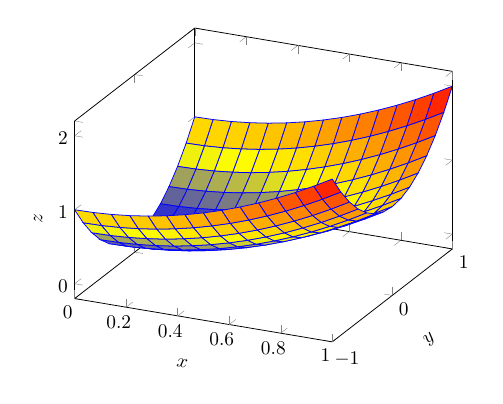
\begin{tikzpicture}[scale=.7]
		\begin{axis}[
			xlabel=$x$,
			ylabel=$y$,
			zlabel=$z$,
			xlabel style={sloped},
			ylabel style={sloped},
		]
			\addplot3[
				surf,
				faceted color=blue,
				samples=15,
				domain=0:1,y domain=-1:1
			]{x^2 + y^2};
		\end{axis}
	\end{tikzpicture}
	\caption{}
	\label{figure:解析几何.椭圆抛物面}
\end{figure}

\subsubsection{双曲抛物面}
方程\begin{equation}\label{equation:解析几何.双曲抛物面的一般方程}
	\frac{x^2}{p}-\frac{y^2}{q}=2z,
	\quad p,q>0
\end{equation}
表示的曲面称为\DefineConcept{双曲抛物面}或\DefineConcept{马鞍面}.
它的图形如\cref{figure:解析几何.双曲抛物面} 所示.
它具有下述性质:
\begin{enumerate}
	\item 对称性.
	\(Ozx\)平面和\(Oyz\)平面都是双曲抛物面的对称平面,\(z\)轴是它的对称轴.

	\item 形状.
	双曲抛物面与\(Oxy\)平面的交线为\[
		\left\{ \begin{array}{l}
			\frac{x^2}{p} - \frac{y^2}{q} = 0, \\
			z = 0.
		\end{array} \right.
	\]
	这时一对经过原点的相交直线.

	双曲抛物面与\(Ozx\)平面、\(Oyz\)平面的交线分别为\[
		\left\{ \begin{array}{l}
			x^2 = 2pz, \\
			y = 0,
		\end{array} \right.
		\qquad
		\left\{ \begin{array}{l}
			y^2 = -2qz, \\
			x = 0;
		\end{array} \right.
	\]
	它们都是抛物线.

	用平面\(z=h\ (h\neq0)\)去截此曲面,得到的截口为\[
		\left\{ \begin{array}{l}
			\frac{x^2}{p} - \frac{y^2}{q} = 2h, \\
			z = h.
		\end{array} \right.
	\]
	这是一条双曲线;
	当\(h>0\)时,它的实轴平行于\(x\)轴;
	当\(h<0\)时,它的实轴平行于\(y\)轴.

	当平行移动抛物线\[
		\left\{ \begin{array}{l}
			y^2 = -2qz, \\
			x = 0,
		\end{array} \right.
	\]
	使得它的顶点沿抛物线\[
		\left\{ \begin{array}{l}
			x^2 = 2pz, \\
			y = 0
		\end{array} \right.
	\]移动时,
	便得到马鞍面.
	这是因为,点\(M(x,y,z)\)在此轨迹上的充分必要条件是:
	\(M\)在以抛物线\[
		\left\{ \begin{array}{l}
			x^2 = 2pz, \\
			y = 0
		\end{array} \right.
	\]上的一个点\(M_0(x_0,y_0,z_0)\)为顶点,
	且轴平行于\(z\)轴,
	形状、开口与\[
		\left\{ \begin{array}{l}
			y^2 = -2qz, \\
			x = 0
		\end{array} \right.
	\]一样的抛物线上,即有\[
		\left\{ \begin{array}{l}
			x_0^2 = 2pz_0, \\
			y_0 = 0, \\
			y^2 = -2q(z-z_0), \\
			x = x_0;
		\end{array} \right.
	\]
	消去\(x_0,y_0,z_0\),得到\[
		y^2=-2q\left(z - \frac{x^2}{2p}\right),
	\]
	整理得\[
		\frac{x^2}{p} - \frac{y^2}{q} = 2z.
	\]
\end{enumerate}

\begin{figure}[ht]%双曲抛物面
	\centering
	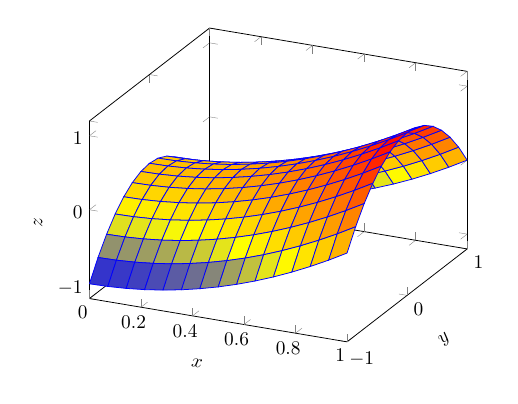
\begin{tikzpicture}[scale=.7]
		\begin{axis}[
			xlabel=$x$,
			ylabel=$y$,
			zlabel=$z$,
			xlabel style={sloped},
			ylabel style={sloped},
		]
			\addplot3[
				surf,
				faceted color=blue,
				samples=15,
				domain=0:1,y domain=-1:1
			]{x^2 - y^2};
		\end{axis}
	\end{tikzpicture}
	\caption{}
	\label{figure:解析几何.双曲抛物面}
\end{figure}

\subsubsection{二次曲面的种类}\label{section:解析几何.二次曲面的种类}
到目前为止,我们学过的二次曲面有以下17种:
\begin{enumerate}[label={\chinese*.}]
	\item 椭球面
	\begin{enumerate}[label={\arabic*.}]
		\item 椭球面:\[
			\frac{x^2}{a^2}+\frac{y^2}{b^2}+\frac{z^2}{c^2}=1;
		\]

		\item 虚椭球面:\[
			\frac{x^2}{a^2}+\frac{y^2}{b^2}+\frac{z^2}{c^2}=-1;
		\]

		\item 点:\[
			\frac{x^2}{a^2}+\frac{y^2}{b^2}+\frac{z^2}{c^2}=0;
		\]
	\end{enumerate}

	\item 双曲面
	\begin{enumerate}[label={\arabic*.}]
		\setcounter{enumii}{3}
		\item 单叶双曲面:\[
			\frac{x^2}{a^2}+\frac{y^2}{b^2}-\frac{z^2}{c^2}=1;
		\]

		\item 双叶双曲面:\[
			\frac{x^2}{a^2}+\frac{y^2}{b^2}-\frac{z^2}{c^2}=-1;
		\]
	\end{enumerate}

	\item 抛物面
	\begin{enumerate}[label={\arabic*.}]
		\setcounter{enumii}{5}
		\item 椭圆抛物面:\[
			\frac{x^2}{p}+\frac{y^2}{q}=2z;
		\]

		\item 双曲抛物面:\[
			\frac{x^2}{p}-\frac{y^2}{q}=2z;
		\]
	\end{enumerate}

	\item 二次锥面
	\begin{enumerate}[label={\arabic*.}]
		\setcounter{enumii}{7}
		\item 二次锥面:\[
			\frac{x^2}{a^2}+\frac{y^2}{b^2}-\frac{z^2}{c^2}=0;
		\]
	\end{enumerate}

	\item 二次柱面
	\begin{enumerate}[label={\arabic*.}]
		\setcounter{enumii}{8}
		\item 椭圆柱面:\[
			\frac{x^2}{a^2}+\frac{y^2}{b^2}=1;
		\]

		\item 虚椭圆柱面:\[
			\frac{x^2}{a^2}+\frac{y^2}{b^2}=-1;
		\]

		\item 直线:\[
			\frac{x^2}{a^2}+\frac{y^2}{b^2}=0;
		\]

		\item 双曲柱面:\[
			\frac{x^2}{a^2}-\frac{y^2}{b^2}=1;
		\]

		\item 一对相交平面:\[
			\frac{x^2}{a^2}-\frac{y^2}{b^2}=0;
		\]

		\item 抛物柱面:\[
			x^2=2py;
		\]

		\item 一对平行平面:\[
			x^2=a^2;
		\]

		\item 一对虚平行平面:\[
			x^2=-a^2;
		\]

		\item 一对重合平面:\[
			x^2=0.
		\]
	\end{enumerate}
\end{enumerate}
我们可以证明二次曲面只有这17种.

不过有的地方也只考虑以下9种曲面是二次曲面:
\begin{enumerate}
	\item 椭圆锥面
	\item 椭球面
	\item 单叶双曲面
	\item 双叶双曲面
	\item 椭圆抛物面
	\item 双曲抛物面
	\item 椭圆柱面
	\item 双曲柱面
	\item 抛物柱面
\end{enumerate}

\subsection{直纹面}
我们看到,柱面和锥面都是由直线组成的.
那么有没有别的也由直线组成的曲面呢?

\begin{definition}
给定一个曲面\(S\),如果存在一族直线,使得这一族中的每一条直线都在\(S\)上,
并且\(S\)上的每一个点都在这一族的某一条直线上,
那么我们称曲面\(S\)为\DefineConcept{直纹面},
称这一族直线为\(S\)的一族\DefineConcept{直母线}.
\end{definition}

二次曲面中哪些是直纹面呢?
9种二次曲面和1种二次锥面都是直纹面.
3种椭球面不是直纹面,因为它有界.
双叶双曲面不是直纹面,
因为当它由方程 \labelcref{equation:解析几何.双叶双曲面} 给出时,
平行于\(Oxy\)平面的直线不可能全在\(S\)上,
与\(Oxy\)平面相交的直线也不会全在\(S\)上.
同理可知,椭圆抛物面不是直纹面.
剩下的2种二次曲面,单叶双曲面和双曲抛物面,可以证明都是直纹面.

\begin{theorem}
单叶双曲面是直纹面.
\begin{proof}
设单叶双曲面\(S\)的方程是\[
	\frac{x^2}{a^2}+\frac{y^2}{b^2}-\frac{z^2}{c^2}=1.
\]
点\(M_0(x_0,y_0,z_0)\)在单叶双曲面\(S\)上的充分必要条件是\[
	\frac{x_0^2}{a^2}+\frac{y_0^2}{b^2}-\frac{z_0^2}{c^2}=1.
\]
移项并且分解因式,得\[
	\left(\frac{x_0}{a}+\frac{z_0}{c}\right)
	\left(\frac{x_0}{a}-\frac{z_0}{c}\right)
	= \left(1+\frac{y_0}{b}\right)
	\left(1-\frac{y_0}{b}\right),
\]
即\[
	\def\arraystretch{1.5}
	\begin{vmatrix}
		\frac{x_0}{a}+\frac{z_0}{c} & 1+\frac{y_0}{b} \\
		1-\frac{y_0}{b} & \frac{x_0}{a}-\frac{z_0}{c}
	\end{vmatrix} = 0.
\]
因为\(1\pm\frac{y_0}{b}\)不全为零,所以方程组\[
	\left\{ \def\arraystretch{1.5} \begin{array}{l}
		\left(\frac{x_0}{a}+\frac{z_0}{c}\right) X
		+ \left(1+\frac{y_0}{b}\right) Y = 0, \\
		\left(1-\frac{y_0}{b}\right) X
		+ \left(\frac{x_0}{a}-\frac{z_0}{c}\right) Y = 0
	\end{array} \right.
\]
是\(X,Y\)的一次齐次方程组.
如前所述,它的系数行列式为零,所以它有非零解,
即存在不全为零的实数\(\mu_0,\nu_0\),使得\[
	\left\{ \def\arraystretch{1.5} \begin{array}{l}
		\mu_0 \left(\frac{x_0}{a}+\frac{z_0}{c}\right)
		+ \nu_0 \left(1+\frac{y_0}{b}\right) = 0, \\
		\mu_0 \left(1-\frac{y_0}{b}\right)
		+ \nu_0 \left(\frac{x_0}{a}-\frac{z_0}{c}\right) = 0.
	\end{array} \right.
\]
这表明点\(M_0\)在直线\[
	l_0: \left\{ \def\arraystretch{1.5} \begin{array}{l}
		\mu_0 \left(\frac{x}{a}+\frac{z}{c}\right)
		+ \nu_0 \left(1+\frac{y}{b}\right) = 0, \\
		\mu_0 \left(1-\frac{y}{b}\right)
		+ \nu_0 \left(\frac{x}{a}-\frac{z}{c}\right) = 0
	\end{array} \right.
\]上.
现在考虑一族直线:\[
	\mathcal{L}:
	\left\{ \def\arraystretch{1.5} \begin{array}{l}
		\mu \left(\frac{x}{a}+\frac{z}{c}\right)
		+ \nu \left(1+\frac{y}{b}\right) = 0, \\
		\mu \left(1-\frac{y}{b}\right)
		+ \nu \left(\frac{x}{a}-\frac{z}{c}\right) = 0,
	\end{array} \right.
\]
其中\(\mu,\nu\)取所有不全为零的实数.
若\((\mu_1,\nu_1)\)与\((\mu_2,\nu_2)\)成比例,
则它们确定直线族\(\mathcal{L}\)中的同一条直线;
若它们不成比例,则它们确定不同的直线.
所以直线族\(\mathcal{L}\)实际上只依赖于一个参数,即\(\mu\)与\(\nu\)的比值.
上面就证明了:
单叶双曲面\(S\)上的任一点\(M_0\)在直线族\(\mathcal{L}\)的某一条直线\(l_0\)上.
现在从直线族\(\mathcal{L}\)中任取一条直线\(l_1\),它对应于\((\mu_1,\nu_1)\),
且在\(l_1\)上任取一点\(M_1(x_1,y_1,z_1)\),则有\[
	\left\{ \def\arraystretch{1.5} \begin{array}{l}
		\mu_1 \left(\frac{x_1}{a}+\frac{z_1}{c}\right)
		+ \nu_1 \left(1+\frac{y_1}{b}\right) = 0, \\
		\mu_1 \left(1-\frac{y_1}{b}\right)
		+ \nu_1 \left(\frac{x_1}{a}-\frac{z_1}{c}\right) = 0.
	\end{array} \right.
\]
因为\(\mu_1,\nu_1\)不全为零,所以上式说明方程组\[
	\left\{ \def\arraystretch{1.5} \begin{array}{l}
		\left(\frac{x_1}{a}+\frac{z_1}{c}\right) X
		+ \left(1+\frac{y_1}{b}\right) Y = 0, \\
		\left(1-\frac{y_1}{b}\right) X
		+ \left(\frac{x_1}{a}-\frac{z_1}{c}\right) Y = 0
	\end{array} \right.
\]有非零解,从而它的系数行列式等于零.
于是可知,\(M_1(x_1,y_1,z_1)\)在单叶双曲面\(S\)上,
也就是说,\(S\)是直纹面,且直线族\(\mathcal{L}\)是它的一族直母线.

考虑到\[
	\def\arraystretch{1.5}
	\begin{vmatrix}
		\frac{x_0}{a}+\frac{z_0}{c} & 1-\frac{y_0}{b} \\
		1+\frac{y_0}{b} & \frac{x_0}{a}-\frac{z_0}{c}
	\end{vmatrix}
	= \begin{vmatrix}
		\frac{x_0}{a}+\frac{z_0}{c} & 1+\frac{y_0}{b} \\
		1-\frac{y_0}{b} & \frac{x_0}{a}-\frac{z_0}{c}
	\end{vmatrix},
\]
我们还可以类似地得到\(S\)的另一族直母线\[
	\left\{ \def\arraystretch{1.5} \begin{array}{l}
		\mu \left(\frac{x}{a}+\frac{z}{c}\right)
		+ \nu \left(1-\frac{y}{b}\right) = 0, \\
		\mu \left(1+\frac{y}{b}\right)
		+ \nu \left(\frac{x}{a}-\frac{z}{c}\right) = 0,
	\end{array} \right.
\]
其中\(\mu,\nu\)取所有不全为零的实数.
\end{proof}
\end{theorem}

\begin{theorem}
双曲抛物面是直纹面.
\begin{proof}
设双曲抛物面\(S\)的方程是\[
	\frac{x^2}{p}-\frac{y^2}{q}=2z,
\]
则它有两族直母线\[
	\left\{ \def\arraystretch{1.5} \begin{array}{l}
		\left(\frac{x}{\sqrt{p}}+\frac{y}{\sqrt{q}}\right)+2\lambda=0, \\
		z+\lambda\left(\frac{x}{\sqrt{p}}-\frac{y}{\sqrt{q}}\right)=0
	\end{array} \right.
	\quad\text{和}\quad
	\left\{ \def\arraystretch{1.5} \begin{array}{l}
		\lambda\left(\frac{x}{\sqrt{p}}+\frac{y}{\sqrt{q}}\right)+z=0, \\
		2\lambda\left(\frac{x}{\sqrt{p}}-\frac{y}{\sqrt{q}}\right)=0,
	\end{array} \right.
\]
其中\(\lambda\)取所有实数.
\end{proof}
\end{theorem}


\subsection{曲面的交线,曲面围成的区域}
\subsubsection{画空间图形常见的三种方法}
在纸上描绘空间图形时,我们常用以下三种方法:
\begin{enumerate}
	\item 斜二测法(或称斜二等轴测投影法).
	让\(z\)轴垂直向上,\(y\)轴水平向右,
	\(x\)轴与\(y\)轴、\(z\)轴分别成 135\textdegree 角.
	规定\(y\)轴与\(z\)轴的单位长度相等,
	而\(x\)轴的单位长度为\(y\)轴单位长度的一半.

	\item 正等测法(即正等轴测投影法).
	让\(z\)轴垂直向上,
	\(x\)轴、\(y\)轴、\(z\)轴两两成 120\textdegree 角.
	规定三根轴的单位长度相等.

	\item 正二测法(即正二等轴测投影法).
	具体地说,有以下两种作图方案:
	\begin{itemize}
		\item 让\(z\)轴垂直向上,
		\(x\)轴与\(z\)轴的夹角为\(90^\circ + \alpha\),
		其中\(\alpha\)是锐角,且\(\tan\alpha\approx\frac{7}{8}\);
		\(y\)轴与\(z\)轴的夹角为\(90^\circ + \beta\),
		其中\(\beta\)是锐角,且\(\tan\beta\approx\frac{1}{8}\).
		规定\(z\)轴和\(y\)轴的单位长度相等,
		而\(x\)轴的单位长度为\(y\)轴的单位长度的一半.

		\item 仍然让\(z\)轴垂直向上,
		\(x\)轴与\(z\)轴夹角为\(90^\circ + \beta\),
		其中\(\tan\beta\approx\frac{1}{8}\);
		\(y\)轴的负向与\(z\)轴的夹角为\(90^\circ + \alpha\),
		其中\(\tan\alpha\approx\frac{7}{8}\).
		规定\(x\)轴与\(z\)轴的单位长度相等,
		\(y\)轴的单位长度为\(z\)轴的单位长度的一半.
	\end{itemize}
	一般来说,采用正二测法画出的图形较为逼真.
\end{enumerate}

\subsubsection{曲线在坐标平面上的投影,曲面的交线的画法}
如\cref{figure:解析几何.点在坐标平面上的投影},
对于空间中任一点\(M\)以及它在三个坐标平面上的投影点\(M_1,M_2,M_3\)这四个点,
只要知道了其中两个点就可以画出另外两个点.
譬如,若知道了\(M_2,M_3\)两个点,则只要分别过\(M_2,M_3\)画出投影线(平行于相应坐标轴的直线),
它们的交点就是点\(M\),再过\(M\)画投影线(平行于\(z\)轴),
它与\(Oxy\)平面的交点就是点\(M_1\).

\begin{figure}[ht]
	\centering
	\begin{tikzpicture}
		\def\spacecoordinate(#1,#2,#3,#4){\coordinate(#1)at(#3-#2*0.35355,#4-#2*0.35355);}%
		\spacecoordinate(O,0,0,0)
		\spacecoordinate(A,1,2,3)
		\spacecoordinate(A1,1,2,0)
		\spacecoordinate(A2,0,2,3)
		\spacecoordinate(A3,1,0,3)

		\begin{scope}[->]
			\draw(O)--(3,0)node[right]{\(y\)};
			\draw(O)--(0,4)node[right]{\(z\)};
			\draw(O)--(-1,-1)node[left]{\(x\)};
		\end{scope}
		\filldraw
			(O)node[above right]{\(O\)}
			(A)circle(2pt)node[right]{\(M\)}
			(A1)circle(2pt)node[right]{\(M_1\)}
			(A2)circle(2pt)node[right]{\(M_2\)}
			(A3)circle(2pt)node[left]{\(M_3\)};
		\draw[dashed]
			(A)--(A1)
			(A)--(A2)
			(A)--(A3);
	\end{tikzpicture}
	\caption{}
	\label{figure:解析几何.点在坐标平面上的投影}
\end{figure}

因此,为了画出两个曲面的交线\(\Gamma\),
只需要先画出\(\Gamma\)上每个点在某两个坐标面上的投影.
\(\Gamma\)上所有点在某个平面\(\alpha\)
(这个平面可以是\(Oxy\)平面、\(Oyz\)平面或\(Ozx\)平面)
上的投影组成的曲线,
称为“\(\Gamma\)在\(\alpha\)上的\DefineConcept{投影曲线}”,
简称为“\(\Gamma\)在\(\alpha\)上的\DefineConcept{投影}”.
如果我们把\(\alpha\)的法线记为\(l\),
把以\(\Gamma\)准线、母线平行于\(l\)的柱面记为\(S\),
那么曲线\(\Gamma\)在\(\alpha\)上的投影就是\(S\)与\(\alpha\)的交线,
我们称柱面\(S\)为“\(\Gamma\)沿\(l\)的\DefineConcept{投影柱面}”.

\subsubsection{曲面所围成的区域的画法}
几个曲面或平面所围成的空间的区域可用几个不等式联立起来表示.
如何画出这个区域呢?
关键是要画出相应曲面的交线,随之可得所求空间区域.

\section{坐标变换}
前两节我们再选定的一个坐标系中研究平面、直线和曲面.
但是,在许多情形下,往往在实现给定的坐标系中一个图形的方程比较复杂,
这时我们需要选择领一个合适的坐标系,使这个图形的方程变得比较简单.
为此,就需要研究同一个点在两个坐标系中的坐标之间的关系.
这样的关系式就称为\DefineConcept{坐标变换公式}.
我们在本节来研究坐标变换公式及其应用.

\subsection{平面的仿射坐标变换}
\subsubsection{点的仿射坐标变换公式}
平面上给了两个仿射坐标系:
\([O;\vb{d}_1,\vb{d}_2]\)
和\([O';\vb{d}_1',\vb{d}_2']\).
为方便起见,前一个称为旧坐标系,简记为 I;
后一个称为新坐标系,简记为 II.
点或向量在 I 中的坐标称为它的旧坐标,
在 II 中的坐标称为它的新坐标.
为了研究同一个点的新旧坐标的关系,
首先要明确上述两个坐标系的相对位置.

设 II 的原点\(O'\)的旧坐标是\((x_0,y_0)\),
基向量\(\vb{d}_1',\vb{d}_2'\)的旧坐标分别是\((a_{11},a_{21})\)和\((a_{12},a_{22})\).
现在我们来求某一点\(M\)的旧坐标\((x,y)\)与它的新坐标\((x',y')\)之间的关系.
因为\begin{align*}
	\vec{OM}
	&= \vec{O O'} + \vec{O' M}
	= (x_0 \vb{d}_1 + y_0 \vb{d}_2)
	+ (x' \vb{d}_1' + y' \vb{d}_2') \\
	&= (x_0 \vb{d}_1 + y_0 \vb{d}_2)
	+ x' (a_{11} \vb{d}_1 + a_{21} \vb{d}_2)
	+ y' (a_{12} \vb{d}_1 + a_{22} \vb{d}_2) \\
	&= (a_{11} x' + a_{12} y' + x_0) \vb{d}_1
	+ (a_{21} x' + a_{22} y' + y_0) \vb{d}_2,
\end{align*}
所以有\begin{equation}\label{equation:解析几何.平面坐标系的点的仿射坐标变换公式I到II}
	\left\{ \begin{array}{l}
		x = a_{11} x' + a_{12} y' + x_0, \\
		y = a_{21} x' + a_{22} y' + y_0.
	\end{array} \right.
\end{equation}
\cref{equation:解析几何.平面坐标系的点的仿射坐标变换公式I到II}
称为“平面上坐标系 I 到 II 的点的\DefineConcept{仿射坐标变换公式}”.
它是一个把任意一点\(M\)的旧坐标\(x,y\)表示成它的新坐标\(x',y'\)的一次多项式.

利用矩阵,我们可以将\cref{equation:解析几何.平面坐标系的点的仿射坐标变换公式I到II}
化为\begin{equation}\label{equation:解析几何.平面坐标系的点的仿射坐标变换公式I到II.矩阵形式1}
	\begin{bmatrix}
		x \\ y
	\end{bmatrix}
	= \begin{bmatrix}
		a_{11} & a_{12} \\
		a_{21} & a_{22}
	\end{bmatrix} \begin{bmatrix}
		x' \\ y'
	\end{bmatrix} + \begin{bmatrix}
		x_0 \\ y_0
	\end{bmatrix}.
\end{equation}
我们称矩阵\[
	\vb{A} = \begin{bmatrix}
		a_{11} & a_{12} \\
		a_{21} & a_{22}
	\end{bmatrix}
\]为“坐标 I 到 II 的\DefineConcept{过渡矩阵}”,
它的第一列是 II 的第一个基向量\(\vb{d}_1'\)的 I 坐标,
第二列是 II 的第二个基向量\(\vb{d}_2'\)的 I 坐标.

\begin{theorem}
平面上点的仿射坐标变换公式 \labelcref{equation:解析几何.平面坐标系的点的仿射坐标变换公式I到II}
中的系数行列式不等于零,即\[
	\begin{vmatrix}
		a_{11} & a_{12} \\
		a_{21} & a_{22}
	\end{vmatrix} \neq 0.
\]
\end{theorem}

根据上述定理,如果我们把\cref{equation:解析几何.平面坐标系的点的仿射坐标变换公式I到II}
看作关于\(x',y'\)的方程组,可以求得唯一解
\begin{equation}\label{equation:解析几何.平面坐标系的点的仿射坐标变换公式II到I}
	\left\{ \begin{array}{l}
		x' = \frac{1}{D} \begin{vmatrix}
			x - x_0 & a_{12} \\
			y - y_0 & a_{22}
		\end{vmatrix}, \\
		y' = \frac{1}{D} \begin{vmatrix}
			a_{11} & x - x_0 \\
			a_{21} & y - y_0
		\end{vmatrix}.
	\end{array} \right.
\end{equation}
其中\[
	D = \begin{vmatrix}
		a_{11} & a_{12} \\
		a_{21} & a_{22}
	\end{vmatrix}.
\]
\cref{equation:解析几何.平面坐标系的点的仿射坐标变换公式II到I}
是把平面上任意一点\(M\)的新坐标\(x',y'\)表示成它的旧坐标\(x,y\)的一次多项式,
我们称其为“平面上坐标系 II 到 I 的点的仿射坐标变换公式”.

\subsubsection{向量的仿射坐标变换公式}
现在我们来看平面上的向量\(\vb{m}\)的旧坐标\((u,v)\)与它的新坐标\((u',v')\)之间的关系.
设\(\vb{m}=\vec{M_1 M_2}\),
其中点\(M_i\)的旧坐标为\((x_i,y_i)\),新坐标为\((x_i',y_i')\ (i=1,2)\),
则有\begin{align*}
	u &= x_2 - x_1
	= (a_{11} x_2' + a_{12} y_2' + x_0)
	- (a_{11} x_1' + a_{12} y_1' + x_0) \\
	&= a_{11} (x_2' - x_1')
	+ a_{12} (y_2' - y_1')
	= a_{11} u' + a_{12} v', \\
	v &= y_2 - y_1
	= (a_{21} x_2' + a_{22} y_2' + y_0)
	- (a_{21} x_1' + a_{22} y_1' + y_0) \\
	&= a_{21} u' + a_{22} v',
\end{align*}
即\begin{equation}\label{equation:解析几何.平面坐标系的向量的仿射坐标变换公式I到II}
	\left\{ \begin{array}{l}
		u = a_{11} u' + a_{12} v', \\
		v = a_{21} u' + a_{22} v'.
	\end{array} \right.
\end{equation}
\cref{equation:解析几何.平面坐标系的向量的仿射坐标变换公式I到II}
称为“平面上坐标系 I 到 II 的向量的仿射坐标变换公式”.
它是把任意一个向量\(\vb{m}\)的旧坐标\(u,v\)表示成它的新坐标\(u',v'\)的一次齐次多项式,
这时与点的坐标变换公式不同的地方.
平面上的点和向量是有本质区别的两种对象,
如果只从一个坐标系来看,
似乎点和向量的坐标都是有序实数对,
看不出它们的区别;
但是,如果取两个原点不重合的仿射坐标系,
通过坐标变换,
就可以看出两者的显著区别:
点的坐标变换公式 \labelcref{equation:解析几何.平面坐标系的点的仿射坐标变换公式I到II} 中有常数项,
而向量的坐标变换公式 \labelcref{equation:解析几何.平面坐标系的向量的仿射坐标变换公式I到II} 中没有常数项.

利用矩阵,我们可以将\cref{equation:解析几何.平面坐标系的向量的仿射坐标变换公式I到II}
化为\begin{equation}\label{equation:解析几何.平面坐标系的向量的仿射坐标变换公式I到II.矩阵形式1}
	\begin{bmatrix}
		u \\ v
	\end{bmatrix}
	= \begin{bmatrix}
		a_{11} & a_{12} \\
		a_{21} & a_{22}
	\end{bmatrix} \begin{bmatrix}
		u' \\ v'
	\end{bmatrix}.
\end{equation}

由于\cref{equation:解析几何.平面坐标系的向量的仿射坐标变换公式I到II}
中的系数行列式仍然不为零,因此可以反解出
\begin{equation}\label{equation:解析几何.平面坐标系的向量的仿射坐标变换公式II到I}
	\left\{ \begin{array}{l}
		u' = \frac{1}{D} \begin{vmatrix}
			u & a_{12} \\
			v & a_{22}
		\end{vmatrix}, \\
		v' = \frac{1}{D} \begin{vmatrix}
			a_{11} & u \\
			a_{21} & v
		\end{vmatrix}.
	\end{array} \right.
\end{equation}
这是“平面上坐标系 II 到 I 的向量的仿射坐标变换公式”.
由\cref{equation:解析几何.平面坐标系的向量的仿射坐标变换公式II到I} 看出,
I 的基向量\(\vb{d}_1,\vb{d}_2\)的 II 坐标分别是\[
	\frac{1}{D} (a_{22},-a_{21}), \qquad
	\frac{1}{D} (-a_{12},a_{11}).
\]

\subsection{平面的直角坐标变换}
设 I \([O;\vb{e}_1,\vb{e}_2]\),II \([O';\vb{e}_1',\vb{e}_2']\)都是直角坐标系.
前一小节关于仿射坐标变换的一般结论和方法对于直角坐标变换都成立,
也就是说我们其实也可以直接应用\cref{%
equation:解析几何.平面坐标系的点的仿射坐标变换公式I到II,%
equation:解析几何.平面坐标系的点的仿射坐标变换公式II到I,%
equation:解析几何.平面坐标系的向量的仿射坐标变换公式I到II,%
equation:解析几何.平面坐标系的向量的仿射坐标变换公式II到I}
进行直角坐标变换.
不过,由于直角坐标系的特殊性,
我们可以对平面上坐标系 II 到 I 的点(或向量)的坐标变换公式进行简化.

\subsubsection{直角坐标变换公式}
设\(O'\)的 I 坐标为\((x_0,y_0)\),
\(\vb{e}_1',\vb{e}_2'\)的 I 坐标分别为\((a_{11},a_{21}),(a_{12},a_{22})\),
则坐标系 I 到 II 的过渡矩阵是\[
	\vb{A} = \begin{bmatrix}
		a_{11} & a_{12} \\
		a_{21} & a_{22}
	\end{bmatrix}.
\]

\begin{theorem}\label{theorem:解析几何.直角坐标变换的过渡矩阵是正交矩阵}
设 I 和 II 都是直角坐标系,
则 I 到 II 的过渡矩阵\(\vb{A}\)是正交矩阵,
并且坐标系 II 到 I 的过渡矩阵是\(\vb{A}^T\).
\begin{proof}
因为\(\abs{\vb{e}_1'}=\abs{\vb{e}_2'}=1\),
\(\vb{e}_1' \perp \vb{e}_2'\),
并且 I 是直角坐标系,
所以有\begin{equation}\label{equation:解析几何.直角坐标变换的过渡矩阵的限定条件}
	\left\{ \begin{array}{l}
		a_{11}^2 + a_{21}^2 = 1, \\
		a_{12}^2 + a_{22}^2 = 1, \\
		a_{11} a_{12} + a_{21} a_{22} = 0.
	\end{array} \right.
\end{equation}
于是\(\vb{A}\)是正交矩阵.
\end{proof}
\end{theorem}

现在依据\cref{theorem:解析几何.直角坐标变换的过渡矩阵是正交矩阵},
我们可以将\cref{equation:解析几何.平面坐标系的点的仿射坐标变换公式II到I,%
equation:解析几何.平面坐标系的向量的仿射坐标变换公式II到I} 改为计算相对简单的以下两个公式:
\begin{equation}\label{equation:解析几何.平面坐标系的点的直角坐标变换公式II到I.矩阵形式1}
	\begin{bmatrix}
		x' \\ y'
	\end{bmatrix}
	= \begin{bmatrix}
		a_{11} & a_{21} \\
		a_{12} & a_{22}
	\end{bmatrix} \begin{bmatrix}
		x - x_0 \\ y - y_0
	\end{bmatrix},
\end{equation}
\begin{equation}\label{equation:解析几何.平面坐标系的向量的直角坐标变换公式II到I.矩阵形式1}
	\begin{bmatrix}
		u' \\ v'
	\end{bmatrix}
	= \begin{bmatrix}
		a_{11} & a_{21} \\
		a_{12} & a_{22}
	\end{bmatrix} \begin{bmatrix}
		u \\ v
	\end{bmatrix}.
\end{equation}

\subsubsection{直角坐标变换的过渡矩阵}
直角坐标系 I 到 II 的过渡矩阵\(\vb{A}\)虽然有四个数,
但是由于它是正交矩阵,
满足\cref{equation:解析几何.直角坐标变换的过渡矩阵的限定条件} 中的三个方程,
因此只有一个数是自由的.
下面来详细讨论这一点.

给定平面上的仿射坐标系\([O;\vb{d}_1,\vb{d}_2]\),
如果从\(\vb{d}_1\)逆时针旋转小于 180\textdegree 的角便与\(\vb{d}_2\)重合,
则称这个坐标系为右手坐标系,简称右手系;
反之,则称之为左手坐标系,简称左手系.
特别地,对于直角坐标系\([O;\vb{e}_1,\vb{e}_2]\)来说,
若\(\vb{e}_1\)旋转 90\textdegree 与\(\vb{e}_2\)重合,则为右手系;
若\(\vb{e}_1\)旋转 -90\textdegree 与\(\vb{e}_2\)重合,则为左手系.

设 I \([O;\vb{e}_1,\vb{e}_2]\),II \([O';\vb{e}_1',\vb{e}_2']\)都是右手直角坐标系,且\[
	O'(x_0,y_0), \qquad
	\vb{e}_1'(a_{11},a_{21}), \qquad
	\vb{e}_2'(a_{12},a_{22}),
\]则有{\def\ExprA#1#2{a_{#1#2} = \vb{e}_#2' \cdot \vb{e}_#1 = \cos\angle(\vb{e}_#2',\vb{e}_#1)}
\begin{align*}
	\ExprA{1}{1}, \qquad
	\ExprA{2}{1}, \\
	\ExprA{1}{2}, \qquad
	\ExprA{2}{2}.
\end{align*}}

\begin{figure}[ht]
	\centering
	\begin{tikzpicture}[->,scale=2]
		\draw(0,0)node[below left]{\(O\)}--(1,0)node[right]{\(\vb{e}_1\)};
		\draw(0,0)--(0,1)node[left]{\(\vb{e}_2\)};
		\begin{scope}[xshift=1.3cm,yshift=1.3cm]
			\draw[dashed,-](0,1)coordinate(E2)--(0,0)coordinate(O)node[below left]{\(O'\)}--(1,0)coordinate(E1);
			\draw(0,0)--(.866,.5)coordinate(E11)node[above right]{\(\vb{e}_1'\)};
			\draw(0,0)--(-.5,.866)coordinate(E22)node[above left]{\(\vb{e}_2'\)};
			\draw pic["\(\theta\)",draw=orange,-,angle eccentricity=1.7,angle radius=5mm]{angle=E1--O--E11};
			\draw pic[draw=orange,-,angle radius=5mm]{angle=E2--O--E22};
		\end{scope}
	\end{tikzpicture}
	\caption{}
	\label{figure:解析几何.平面坐标变换的过渡矩阵与旋转角的关系}
\end{figure}

如\cref{figure:解析几何.平面坐标变换的过渡矩阵与旋转角的关系},
设\(\vb{e}_1\)逆时针旋转\(\theta\)角便与\(\vb{e}_1'\)重合,
在\[
	0 \leq \theta < \frac{\pi}{2}, \qquad
	\frac{\pi}{2} \leq \theta < \pi, \qquad
	\pi \leq \theta < \frac{3}{2}\pi, \qquad
	\frac{3}{2}\pi \leq \theta < 2\pi
\]这四种情况下,总可得\[
	a_{11} = \cos\theta, \qquad
	a_{21} = \sin\theta, \qquad
	a_{12} = -\sin\theta, \qquad
	a_{22} = \cos\theta,
\]
那么 I 到 II 的过渡矩阵为\[
	\vb{A} = \begin{bmatrix}
		\cos\theta & -\sin\theta \\
		\sin\theta & \cos\theta
	\end{bmatrix}.
\]
应该注意到,\(\abs{\vb{A}}=1\).

类似地,设\(\theta\)仍表示\(\vb{e}_1\)到\(\vb{e}_1'\)的转角,
若 I 是右手直角坐标系,而 II 是左手直角坐标系,
则 I 到 II 的过渡矩阵为\[
	\begin{bmatrix}
		\cos\theta & \sin\theta \\
		\sin\theta & -\cos\theta
	\end{bmatrix};
\]
若 I 是左手直角坐标系,而 II 是右手直角坐标系,
则 I 到 II 的过渡矩阵为\[
	\begin{bmatrix}
		\cos\theta & -\sin\theta \\
		-\sin\theta & -\cos\theta
	\end{bmatrix};
\]
若 I 和 II 都是左手直角坐标系,
则 I 到 II 的过渡矩阵为\[
	\begin{bmatrix}
		\cos\theta & \sin\theta \\
		-\sin\theta & \cos\theta
	\end{bmatrix}.
\]

\begin{definition}
给定平面(或空间)的两个坐标系,
如果它们都是右手系,或者它们都是左手系,
则称它们是\DefineConcept{同定向的};
如果一个是左手系,另一个是右手系,
则称它们是\DefineConcept{反定向的}.
\end{definition}

从上面的讨论可以得到
\begin{theorem}
设 I 和 II 都是平面的直角坐标系,
I 到 II 的过渡矩阵是\(\vb{A}\),
则 I 和 II 同定向的充分必要条件是\(\abs{\vb{A}}=1\),
从而它们反定向的充分必要条件是\(\abs{\vb{A}}=-1\).
\end{theorem}

如无特别声明,今后所取的直角坐标系都是右手系.

\subsubsection{移轴公式和转轴公式}
设 I \([O;\vb{e}_1,\vb{e}_2]\),II \([O';\vb{e}_1',\vb{e}_2']\)都是右手直角坐标系,
\(O'(x_0,y_0)\),
\(\vb{e}_1\)到\(\vb{e}_1'\)的转角为\(\theta\),
则 I 到 II 的点的坐标变换公式为
\begin{equation}\label{equation:解析几何.平面坐标系的点的右手直角坐标变换公式I到II.矩阵形式1}
	\begin{bmatrix}
		x \\ y
	\end{bmatrix} = \begin{bmatrix}
		\cos\theta & -\sin\theta \\
		\sin\theta & \cos\theta
	\end{bmatrix} \begin{bmatrix}
		x' \\ y'
	\end{bmatrix} + \begin{bmatrix}
		x_0 \\ y_0
	\end{bmatrix}.
\end{equation}

若\(\theta=0\),
则\cref{equation:解析几何.平面坐标系的点的右手直角坐标变换公式I到II.矩阵形式1} 成为
\begin{equation}\label{equation:解析几何.平面坐标系的点的右手直角坐标变换公式I到II.矩阵形式2}
	\begin{bmatrix}
		x \\ y
	\end{bmatrix} = \begin{bmatrix}
		1 & 0 \\
		0 & 1
	\end{bmatrix} \begin{bmatrix}
		x' \\ y'
	\end{bmatrix} + \begin{bmatrix}
		x_0 \\ y_0
	\end{bmatrix},
\end{equation}
即\begin{equation}\label{equation:解析几何.平面坐标系的点的右手直角坐标变换公式I到II.代数形式2}
	\left\{ \begin{array}{l}
		x = x' + x_0, \\
		y = y' + y_0.
	\end{array} \right.
\end{equation}
\cref{equation:解析几何.平面坐标系的点的右手直角坐标变换公式I到II.矩阵形式2,%
equation:解析几何.平面坐标系的点的右手直角坐标变换公式I到II.代数形式2}
称为\DefineConcept{移轴公式}.

若\(O'\)与\(O\)重合,
则\cref{equation:解析几何.平面坐标系的点的右手直角坐标变换公式I到II.矩阵形式1} 成为
\begin{equation}\label{equation:解析几何.平面坐标系的点的右手直角坐标变换公式I到II.矩阵形式3}
	\begin{bmatrix}
		x \\ y
	\end{bmatrix} = \begin{bmatrix}
		1 & 0 \\
		0 & 1
	\end{bmatrix} \begin{bmatrix}
		x' \\ y'
	\end{bmatrix}.
\end{equation}
\cref{equation:解析几何.平面坐标系的点的右手直角坐标变换公式I到II.矩阵形式3}
称为\DefineConcept{转轴公式}.

\cref{equation:解析几何.平面坐标系的点的右手直角坐标变换公式I到II.矩阵形式1,%
equation:解析几何.平面坐标系的点的右手直角坐标变换公式I到II.矩阵形式2,%
equation:解析几何.平面坐标系的点的右手直角坐标变换公式I到II.矩阵形式3}
说明,平面上任一右手直角坐标变换可以经过移轴和转轴得到,
即对于右手直角坐标系 I \([O;\vb{e}_1,\vb{e}_2]\) 和 II \([O';\vb{e}_1',\vb{e}_2']\),有\[
	[O;\vb{e}_1,\vb{e}_2]
	\xlongrightarrow{\text{移轴}}
	[O';\vb{e}_1,\vb{e}_2]
	\xlongrightarrow{\text{转轴}}
	[O';\vb{e}_1',\vb{e}_2']
\]或\[
	[O;\vb{e}_1,\vb{e}_2]
	\xlongrightarrow{\text{转轴}}
	[O;\vb{e}_1',\vb{e}_2']
	\xlongrightarrow{\text{移轴}}
	[O';\vb{e}_1',\vb{e}_2'].
\]

上述结论对于任意两个同定向的直角坐标系仍成立,但对于反定向的两个直角坐标系不成立.

\subsection{空间的仿射坐标变换}
\begin{theorem}\label{theorem:解析几何.空间的仿射坐标变换公式}
设 I \([O;\vb{d}_1,\vb{d}_2,\vb{d}_3]\)
和 II \([O';\vb{d}_1',\vb{d}_2',\vb{d}_3']\)
都是空间仿射坐标系,
\(O'\)的 I 坐标是\((x_0,y_0,z_0)\),
\(\vb{d}_j'\)的 I 坐标是\((a_{1j},a_{2j},a_{3j})\ (j=1,2,3)\),
则 I 到 II 的点的仿射坐标变换公式为
\begin{equation}
	\begin{bmatrix}
		x \\ y \\ z
	\end{bmatrix} = \begin{bmatrix}
		a_{11} & a_{12} & a_{13} \\
		a_{21} & a_{22} & a_{23} \\
		a_{31} & a_{32} & a_{33}
	\end{bmatrix} \begin{bmatrix}
		x' \\ y' \\ z'
	\end{bmatrix} + \begin{bmatrix}
		x_0 \\ y_0 \\ z_0
	\end{bmatrix},
\end{equation}
I 到 II 的向量的仿射坐标变换公式为
\begin{equation}
	\begin{bmatrix}
		u_1 \\ u_2 \\ u_3
	\end{bmatrix} = \begin{bmatrix}
		a_{11} & a_{12} & a_{13} \\
		a_{21} & a_{22} & a_{23} \\
		a_{31} & a_{32} & a_{33}
	\end{bmatrix} \begin{bmatrix}
		u_1' \\ u_2' \\ u_3'
	\end{bmatrix},
\end{equation}
其中\[
	\vb{A} = \begin{bmatrix}
		a_{11} & a_{12} & a_{13} \\
		a_{21} & a_{22} & a_{23} \\
		a_{31} & a_{32} & a_{33}
	\end{bmatrix}
\]称为“I 到 II 的过渡矩阵”,
它的第\(j\)列是\(\vb{d}_j'\ (j=1,2,3)\)的 I 坐标.
\end{theorem}

\begin{theorem}\label{theorem:解析几何.空间仿射坐标系同定向的充分必要条件}
仿射坐标系 I \([O;\vb{d}_1,\vb{d}_2,\vb{d}_3]\)
到 II \([O';\vb{d}_1',\vb{d}_2',\vb{d}_3']\)的过渡矩阵\(\vb{A}\)是非奇异的,
并且 I 与 II 同定向的充分必要条件是\(\abs{A}>0\).
\end{theorem}

\begin{corollary}
平面上的两个仿射坐标系 I \([O;\vb{d}_1,\vb{d}_2]\)
和 II \([O';\vb{d}_1',\vb{d}_2']\)同定向的充分必要条件是:
I 到 II 的过渡矩阵\(\vb{A}\)的行列式\(\abs{A}>0\).
\end{corollary}

\subsection{空间的直角坐标变换}
\cref{theorem:解析几何.空间的仿射坐标变换公式,%
theorem:解析几何.空间仿射坐标系同定向的充分必要条件}
在直角坐标系中当然也成立,
现在我们进一步研究直角坐标变换的特殊性.

\begin{theorem}
设 I \([O;\vb{e}_1,\vb{e}_2,\vb{e}_3]\)
和 II \([O';\vb{e}_1',\vb{e}_2',\vb{e}_3']\)
都是直角坐标系,
则 I 到 II 的过渡矩阵\(\vb{A}\)是正交矩阵,
从而 II 到 I 的过渡矩阵是\(\vb{A}^T\).
\end{theorem}

由于正交矩阵的行列式等于\(\pm1\),
因此空间的两个直角坐标系同定向的充分必要条件就是它们的过渡矩阵的行列式等于\(+1\).

\subsection{代数曲面、代数曲线及其次数}
空间(或平面)的任一点对于不同不同坐标系的坐标是不同的,
因而作为点的轨迹的图形在不同坐标系中的方程也就不同,但是有
\begin{theorem}\label{theorem:解析几何.坐标变换时代数图形的不变性}
若图形\(S\)在仿射坐标系 I 中的方程\(F(x,y,z)=0\)的左端是关于\(x,y,z\)的\(n\)次多项式,
则\(S\)在任意一个仿射坐标系 II 中的方程\(G(x',y',z')=0\)的左端是关于\(x',y',z'\)的\(n\)次多项式.
\end{theorem}
\cref{theorem:解析几何.坐标变换时代数图形的不变性} 说明,
一个图形的方程的左端是否为多项式,以及这个多项式的次数与坐标系的选择无关,
它们都是图形本身的性质.

若图形\(S\)的左端是多项式,则称\(S\)为\DefineConcept{代数曲面},
并且把这个多项式的次数称为这个代数曲面的\DefineConcept{次数}.

平面上的图形有类似的性质.
若平面上图形\(S\)的方程\(F(x,y)=0\)的左端是多项式,
则称\(S\)是\DefineConcept{代数曲线},
并且把这个多项式的次数称为这个代数曲线的\DefineConcept{次数}.
例如,椭圆、双曲线、抛物线在直角坐标系中的标准方程是二次的,
由此可知,它们不论在哪一个仿射坐标系中的方程也都是二次的,
所以它们才都被称为二次曲线.


\section{本章总结}
\subsection*{向量及其运算}
\begin{table}[ht]
	\centering
	\begin{tabular}{|c|c|c|c|}
	\hline
	\multicolumn{2}{|c|}{加法} & \multicolumn{2}{c|}{数乘} \\ \hline
	交换律 & \(\vb{a}+\vb{b}=\vb{b}+\vb{a}\) &
		结合律 & \(\lambda(\mu\vb{a})=\mu(\lambda\vb{a})=(\lambda\mu)\vb{a}\) \\ \hline
	\multirow{2}{*}{结合律} & \multirow{2}{*}{\((\vb{a}+\vb{b})+\vb{c}=\vb{a}+(\vb{b}+\vb{c})\)} &
		\multirow{2}{*}{分配律} & \((\lambda+\mu)\vb{a}=\lambda\vb{a}+\mu\vb{a}\) \\
	 & & & \(\lambda(\vb{a}+\vb{b})=\lambda\vb{a}+\lambda\vb{b}\) \\ \hline
	\multicolumn{2}{|c|}{点乘} & \multicolumn{2}{c|}{叉乘} \\ \hline
	交换律 & \(\vb{a}\cdot\vb{b}=\vb{b}\cdot\vb{a}\) &
		负交换律 & \(\vb{a}\times\vb{b}=-\vb{b}\times\vb{a}\) \\ \hline
	分配律 & \((\vb{a}+\vb{b})\cdot\vb{c}=\vb{a}\cdot\vb{c}+\vb{b}\cdot{c}\) &
		分配律 & \((\vb{a}+\vb{b})\times\vb{c}=\vb{a}\times\vb{c}+\vb{b}\times\vb{c}\) \\ \hline
	\multirow{3}{*}{结合律} & \((\lambda\vb{a})\cdot\vb{b}=\lambda(\vb{a}\cdot\vb{b})\) & \multirow{3}{*}{结合律} & \multirow{3}{*}{\((\lambda\vb{a})\times\vb{b}=\vb{a}\times(\lambda\vb{b})=\lambda(\vb{a}\times\vb{b})\)} \\
		& \(\vb{a}\cdot(\lambda\vb{b})=\lambda(\vb{a}\cdot\vb{b})\) & & \\
		& \((\lambda\vb{a})\cdot(\mu\vb{b})=\lambda\mu(\vb{a}\cdot\vb{b})\) & & \\
	\hline
	\end{tabular}
	\caption{向量的运算法则}
\end{table}

\subsection*{常见的坐标系}
极坐标系是一种平面坐标系.
极坐标系上的点\((\rho,\theta)\)与平面直角坐标系上的点\((x,y)\)存在以下的一一对应关系:\[
\left\{ \begin{array}{l}
x = \rho\cos\theta, \\
y = \rho\sin\theta. \\
\end{array} \right.
\]

柱面坐标系是一种空间坐标系.
柱面坐标系上的点\((\rho,\theta,z)\)与空间直角坐标系上的点\((x,y,z)\)存在以下的一一对应关系:\[
\left\{ \begin{array}{l}
x = \rho\cos\theta, \\
y = \rho\sin\theta, \\
z = z. \\
\end{array} \right.
\]

球极坐标系是一种空间坐标系.
球极坐标系上的点\((r,\theta,\phi)\)与空间直角坐标系上的点\((x,y,z)\)存在以下的一一对应关系:\[
\left\{ \begin{array}{l}
x = r \sin\phi \cos\theta, \\
y = r \sin\phi \sin\theta, \\
z = r \cos\phi. \\
\end{array} \right.
\]

\begin{figure}[h]
	\centering
	\begin{tikzpicture}
		\coordinate (O) at (0,0);
		\coordinate (M) at (2,2);
		\coordinate (P) at (2,-1.2);
		\coordinate (A) at (-0.8,-1.2);
		\coordinate (Z) at (0,1);
		\draw (O)node[left]{\(O\)}
				-- (M)node[right]{\(M\)} node[midway,above]{\(r\)}
				-- (P)node[right]{\(P\)} node[midway,right]{\(z\)}
				-- (A)node[left]{\(A\)} node[midway,below]{\(y\)}
				-- (O)node[midway,left]{\(x\)}
			(O) -- (P)
			pic["\(\phi\)",draw=orange,<-,angle eccentricity=1.3,angle radius=0.6cm]{angle=M--O--Z}
			pic["\(\theta\)",draw=orange,->,angle eccentricity=1.5,angle radius=0.4cm]{angle=A--O--P};
		\begin{scope}[>=Stealth,->,ultra thick]
			\draw(0,0) -- (-1.5,-2.25) node[right]{\(x\)};
			\draw(0,0) -- (3,0) node[right]{\(y\)};
			\draw(0,0) -- (0,3) node[above]{\(z\)};
		\end{scope}
	\end{tikzpicture}
	\caption{球极坐标系}
\end{figure}

\subsection*{常见二次曲面}
具体见\pagecref{section:解析几何.二次曲面的种类}.


\chapter{函数}
\section{函数的概念}
\subsection{一元函数的概念}
设\(D\)是\(\mathbb{R}\)的一个非空子集,
称映射\(f\colon D \to \mathbb{R}\)为
“定义在\(D\)上的一个\DefineConcept{一元函数}(univariate function)”,
%@see: https://mathworld.wolfram.com/UnivariateFunction.html
简称\DefineConcept{函数},通常记为\[
	y = f(x), \qquad x \in D,
\]
其中点集\(D\)称为该函数的\DefineConcept{定义域},
\(x\)称为\DefineConcept{自变量},
\(y\)称为\DefineConcept{因变量}.

函数定义中,对每个\(x \in D\),
按对应法则\(f\),总有唯一确定的值\(y\)与之相应,
这个值称为函数\(f\)在\(x\)处的\DefineConcept{函数值},
记作\(f(x)\),即\(y=f(x)\).
因变量\(y\)与自变量\(x\)之间的这种依赖关系,通常称为\DefineConcept{函数关系}.
函数值\(f(x)\)的全体所构成的集合称为函数\(f\)的\DefineConcept{值域},
记作\(R_f\)或\(f\ImageOfSetUnderRelation{D}\),即\[
	R_f = f\ImageOfSetUnderRelation{D} = \Set{ y \given y = f(x) \land x \in D }.
\]

函数的定义域通常按以下两种情形来确定:
\begin{itemize}
	\item 一种是对有实际背景的函数,
	根据实际背景中变量的实际意义来确定.
	\item 另一种是对抽象地用算式表达的函数,
	通常约定这种函数的定义域是使得算式有意义的一切实数组成的集合,
	这种定义域称为函数的\DefineConcept{自然定义域}.
\end{itemize}

\begin{example}
函数\(y = \frac{1}{x}\)的自然定义域是
\(\Set{ x \in \mathbb{R} \given x \neq 0 }\).
\end{example}

\begin{example}
函数\(y = \sqrt{x}\)的自然定义域是
\(\Set{ x \in \mathbb{R} \given x \geq 0 }\).
\end{example}

如果给定一个对应法则,按这个法则,
对每个\(x \in D\),总有确定但不唯一的\(y\)与之对应.
这样的不符合函数的定义的对应法则,
习惯上称这种法则确定了一个\DefineConcept{多值函数}.
对于多值函数,如果我们附加一些条件,使得在附加条件之下,按照这个法则,
对每个\(x \in D\),总有唯一确定的实数值\(y\)与之对应,那么这就确定了一个函数.
我们称这样得到的函数为多值函数的\DefineConcept{单值分支}.

\subsection{多元函数的概念}
\begin{definition}
设\(D\)是\(\mathbb{R}^2\)的一个非空子集,
称映射\(f\colon D \to \mathbb{R}\)为
“定义在\(D\)上的\DefineConcept{二元函数}”,
通常记为\[
	z = f(x,y),
	\quad (x,y) \in D
\]或\[
	z = f(P),
	\quad P(x,y) \in D
\]
其中点集\(D\)称为该函数的\DefineConcept{定义域},
\(x\)、\(y\)称为\DefineConcept{自变量},
\(z\)称为\DefineConcept{因变量}.
\end{definition}

\begin{definition}
类似地,设\(D\)是\(n\)维空间\(\mathbb{R}^n\)的一个非空子集,
称映射\[
	f\colon D \to \mathbb{R}
\]
为“定义在\(D\)上的\(n\)元\DefineConcept{函数}”,
通常记为\[
	y = f(\AutoTuple{x}{n}),
	\quad \opair{\AutoTuple{x}{n}} \in D
\]或\[
	y = f(\vb{x}),
	\quad \vb{x}=\opair{\AutoTuple{x}{n}} \in D
\]
其中点集\(D\)称为“函数\(f\)的\DefineConcept{定义域}”,
\(x\)、\(y\)称为“函数\(f\)的\DefineConcept{自变量}”,
\(z\)称为“函数\(f\)的\DefineConcept{因变量}”.
\end{definition}
%@see: https://mathworld.wolfram.com/MultivariateFunction.html

\section{函数的性质}
\subsection{函数的有界性}
\begin{definition}\label{definition:函数.函数的有界性}
%@see: 《数学分析(上册)》(陈纪修) P19 定义1.2.3
设函数\(f\)的定义域为\(D\),数集\(X \subseteq D\).

如果存在数\(K_1\),使得\(f(x) \leq K_1\)对任一\(x \in X\)都成立,即\[
	(\forall x \in X)
	(\exists K_1 \in \mathbb{R})
	[f(x) \leq K_1],
\]
则称“函数\(f\)在\(X\)上有\DefineConcept{上界}”,
称“\(K_1\)是函数\(f\)在\(X\)上的一个上界”.

如果存在数\(K_2\),使得\(f(x) \geq K_2\)对任一\(x \in X\)都成立,即\[
	(\forall x \in X)
	(\exists K_2 \in \mathbb{R})
	[f(x) \geq K_2],
\]
则称“函数\(f\)在\(X\)上有\DefineConcept{下界}”,
称“\(K_2\)是函数\(f\)在\(X\)上的一个下界”.

如果存在正数\(M\),使得\(\abs{f(x)} \leq M\)对任一\(x \in X\)都成立,即\[
	(\forall x \in X)
	(\exists M>0)[
		\abs{f(x)} \leq M
	],
\]
则称“函数\(f\)在\(X\)上\DefineConcept{有界}”
或“函数\(f\)是\(X\)上的\DefineConcept{有界函数}”.
反之如果这样的\(M\)不存在,即\[
	(\exists x_0 \in X)
	(\forall M>0)[
		\abs{f(x_0)} > M
	],
\]
就称“函数\(f\)在\(X\)上\DefineConcept{无界}”.
\end{definition}

应该注意到,当一个函数有界时,它的上界、下界均不唯一.
对于一个上界为\(M\)、下界为\(m\)的函数,
任意小于\(m\)的数都是它的下界,
任意大于\(M\)的数都是它的上界.

\begin{theorem}
设函数\(f\)的定义域为\(D\),数集\(X \subseteq D\).
函数\(f\)在\(X\)上有界的充分必要条件是它在\(X\)上既有上界又有下界.
\end{theorem}

\subsection{函数的单调性}
\begin{definition}
%@see: 《数学分析(上册)》(陈纪修) P20 定义1.2.4
设函数\(f\)的定义域为\(D\),区间\(I \subseteq D\).
\begin{itemize}
	\item 如果\[
		(\forall x_1,x_2\in I)
		[x_1 < x_2 \implies f(x_1) \leq f(x_2)],
	\]
	则称“函数\(f\)在区间\(I\)上是\DefineConcept{单调增加的}”.

	\item 如果\[
		(\forall x_1,x_2\in I)
		[x_1 < x_2 \implies f(x_1) < f(x_2)],
	\]
	则称“函数\(f\)在区间\(I\)上是\DefineConcept{严格单调增加的}”.

	\item 如果\[
		(\forall x_1,x_2\in I)
		[x_1 < x_2 \implies f(x_1) \geq f(x_2)],
	\]
	则称“函数\(f\)在区间\(I\)上是\DefineConcept{单调减少的}”.

	\item 如果\[
		(\forall x_1,x_2\in I)
		[x_1 < x_2 \implies f(x_1) > f(x_2)],
	\]
	则称“函数\(f\)在区间\(I\)上是\DefineConcept{严格单调减少的}”.
\end{itemize}

单调增加的函数和单调减少的函数统称为\DefineConcept{单调函数}(monotonic function).
%@see: https://mathworld.wolfram.com/MonotonicFunction.html
\end{definition}

\begin{proposition}
“\(f\)是单调函数”是“\(f\)是单射”的充分不必要条件.
\end{proposition}

\subsection{函数的奇偶性}
\begin{definition}
%@see: 《数学分析(上册)》(陈纪修) P20 定义1.2.5
设函数\(f\)定义域\(D\)关于原点对称,即\((\forall x)[x \in D \iff -x \in D]\).
\begin{itemize}
	\item 若\((\forall x \in D)
	[f(-x) = f(x)]\),
	则称“\(f\)是\DefineConcept{偶函数}”.

	\item 若\((\forall x \in D)
	[f(-x) = -f(x)]\),
	则称“\(f\)是\DefineConcept{奇函数}”.

	\item 若\(f\)既不是奇函数也不是偶函数,
	则称“\(f\)是\DefineConcept{非奇非偶函数}”.
\end{itemize}
\end{definition}

\begin{property}
偶函数的图形是关于\(y\)轴对称的.
奇函数的图形是关于原点对称的.
\end{property}

\begin{property}
奇函数与奇函数之和、之差均为奇函数.
偶函数与偶函数之和、之差均为偶函数.
\begin{proof}
设\[
f(-x) = -f(x), \qquad g(-x) = -g(x).
\]令\(F(x) = f(x) \pm g(x)\),则\[
F(-x) = f(-x) \pm g(-x)
= [-f(x)] \pm [-g(x)]
= -[f(x) \pm g(x)]
= -F(x).
\qedhere
\]
\end{proof}
\end{property}

\begin{property}
奇函数与奇函数之积为偶函数.
\begin{proof}
设\[
f(-x) = -f(x), \qquad g(-x) = -g(x).
\]令\(F(x) = f(x) \cdot g(x)\),则\[
F(-x) = f(-x) \cdot g(-x)
= [-f(x)] \cdot [-g(x)]
= f(x) \cdot g(x)
= F(x).
\qedhere
\]
\end{proof}
\end{property}

\begin{property}
奇函数与偶函数之积为奇函数.
\begin{proof}
设\[
f(-x) = -f(x), \qquad g(-x) = g(x).
\]令\(F(x) = f(x) \cdot g(x)\),则\[
F(-x) = f(-x) \cdot g(-x)
= [-f(x)] \cdot g(x)
= - f(x) \cdot g(x)
= - F(x).
\qedhere
\]
\end{proof}
\end{property}

\begin{property}
偶函数与偶函数之积为偶函数.
\begin{proof}
设\[
f(-x) = f(x), \qquad g(-x) = g(x).
\]令\(F(x) = f(x) \cdot g(x)\),则\[
F(-x) = f(-x) \cdot g(-x) = f(x) \cdot g(x) = F(x).
\qedhere
\]
\end{proof}
\end{property}

\begin{example}\label{example:函数.任一函数可拆为奇偶函数之和}
试证:任意一个函数总可分解为一个奇函数与一个偶函数之和.
\begin{proof}
设函数\(f\colon(-l,l)\to\mathbb{R}\),其中\(l>0\).
假设在\((-l,l)\)上存在偶函数\(g\)和奇函数\(h\),
使得\[
	(\forall x)
	[-l<x<l \implies f(x) = g(x)+h(x)].
\]
那么可以建立关于\(g(x),h(x)\)的方程\[
	\left\{ \begin{array}{l}
		f(x) = g(x) + h(x), \\
		f(-x) = g(-x) + h(-x) = g(x) - h(x).
	\end{array} \right.
\]
解得\[
	g(x) = \frac12 [f(x) + f(-x)], \qquad
	h(x) = \frac12 [f(x) - f(-x)].
\]
可以验证:\[
	g(-x) = \frac12 [f(-x) + f(x)] = g(x), \qquad
	h(-x) = \frac12 [f(-x) - f(x)] = -h(x).
\]
也就是说,\(g\)是偶函数,\(h\)是奇函数.
\end{proof}
\end{example}

\begin{example}
设函数\(f\colon\mathbb{R}\to\mathbb{R}\)
满足\((\forall x\in\mathbb{R})[f(x)\neq0]\).
证明:\[
	\frac{f(x)}{f(-x)} = \left\{ \begin{array}{rl}
		-1, & \text{$f$是奇函数}, \\
		1, & \text{$f$是偶函数}.
	\end{array} \right.
\]
\begin{proof}
假设\(f\)是奇函数,
即\(f(-x)=-f(x)\),
那么\[
	\frac{f(x)}{f(-x)}
	=\frac{f(x)}{-f(x)}
	=-1.
\]

假设\(f\)是偶函数,
即\(f(-x)=f(x)\),
那么\[
	\frac{f(x)}{f(-x)}
	=\frac{f(x)}{f(x)}
	=1.
	\qedhere
\]
\end{proof}
\end{example}

\begin{example}
设函数\(f\colon\mathbb{R}\to\mathbb{R}\).
证明:\[
	f(x) \cdot f(-x) = \left\{ \begin{array}{rl}
		f^2(x), & \text{$f$是偶函数}, \\
		-f^2(x), & \text{$f$是奇函数}.
	\end{array} \right.
\]
\begin{proof}
假设\(f\)是奇函数,
即\(f(-x)=-f(x)\),
那么\[
	f(x) \cdot f(-x)
	=f(x) \cdot (-f(x))
	=-f^2(x).
\]

假设\(f\)是偶函数,
即\(f(-x)=f(x)\),
那么\[
	f(x) \cdot f(-x)
	=f(x) \cdot f(x)
	=f^2(x).
	\qedhere
\]
\end{proof}
\end{example}

\subsection{函数的周期性}
\begin{definition}
%@see: 《数学分析(上册)》(陈纪修) P20 定义1.2.6
设函数\(f\colon D\to\mathbb{R}\).
如果存在一个常数\(T>0\),
使得\[
	(\forall x \in D)
	[x+T \in D \implies f(x+T) = f(x)],
\]
则称“\(f\)是一个\DefineConcept{周期函数}(periodic function)”
“\(f\)是一个以\(T\)为周期的函数”
“\(T\)是\(f\)的\DefineConcept{周期}(period)”.
%@see: https://mathworld.wolfram.com/PeriodicFunction.html
\end{definition}

\begin{definition}
设\(f\)是一个以\(T\)为周期的函数.
如果\[
	(\forall a\in\mathbb{R})
	[0<a<T \implies f(x+a) \neq f(x)],
\]
则称“\(T\)是\(f\)的\DefineConcept{最小正周期}(least period)”
“\(f\)存在最小正周期”;
否则称“\(f\)不存在最小正周期”.
%@see: https://mathworld.wolfram.com/LeastPeriod.html
\end{definition}

\begin{example}\label{example:函数的性质.周期性.常数函数}
常数函数\(f(x) = 0\)是一个周期函数,它以任意正数为周期.
\end{example}

\begin{example}\label{example:函数的性质.周期性.狄利克雷函数}
狄利克雷函数\[
	D(x) = \left\{ \begin{array}{ll}
		1, & x \in \mathbb{Q}, \\
		0, & x \in \mathbb{R}-\mathbb{Q}.
	\end{array} \right.
\]是一个周期函数,任何正有理数\(r\)都是它的周期.
因为不存在最小的正有理数,所以它没有最小正周期.
\end{example}

\begin{remark}
从\cref{example:函数的性质.周期性.常数函数,example:函数的性质.周期性.狄利克雷函数}
可以看出:周期函数不一定存在最小正周期.
\end{remark}

\begin{example}
设函数\(f\colon\mathbb{R}\to\mathbb{R}\)满足\[
	f(x+a) = -f(x),
	\quad a\neq0,
\]
证明:函数\(f\)的周期为\(2a\).
\begin{proof}
易见\(f(x+2a)
=f((x+a)+a)
=-f(x+a)
=f(x)\).
\end{proof}
\end{example}

\begin{example}
设函数\(f\colon\mathbb{R}\to\mathbb{R}\)同时满足\[
	f(x)=f(2a-x)
	\quad\text{和}\quad
	f(x)=f(2b-x),
\]
证明:函数\(f\)的周期为\(2\abs{a-b}\).
\begin{proof}
易见\(f(x)
=f(2a-x)
=f(2b-x)\).
令\(t=2b-x\),
得\(x=2b-t\),
故\(f(2a-(2b-t))=f(t)\),
即\(f(t)=f(t+2(a-b))\).
\end{proof}
\end{example}

\begin{example}
设函数\(f\colon\mathbb{R}\to\mathbb{R}\)同时满足\[
	f(x)+f(2a-x)=0
	\quad\text{和}\quad
	f(x)=f(2b-x),
\]
证明:函数\(f\)的周期为\(4\abs{a-b}\).
\begin{proof}
易见\(f(2b-x)+f(2a-x)=0\).
令\(t=2b-x\),
则\[
	f(t)+f(2a-(2b-t))
	=f(t)+f(t+2(a-b))
	=0.
	\qedhere
\]
\end{proof}
\end{example}

\begin{example}
设函数\(f\colon\mathbb{R}\to\mathbb{R}\)满足\[
	f(x+a)=\pm\frac1{f(x)},
\]
证明:函数\(f\)的周期为\(2\abs{a}\).
\begin{proof}
易见\(f(x+2a)=\pm\frac1{f(x+a)}=f(x)\).
\end{proof}
\end{example}

\section{反函数与复合函数}
\subsection{反函数}
根据\cref{theorem:集合论.关系及其逆是映射的充分必要条件},
当函数\(f\colon X \to Y\)是单射时,
它有逆映射\(f^{-1}\).
\(f^{-1}\)的定义域和值域分别为\(Z=\ran f\)和\(\dom f=X\).
我们把这个逆映射称为“函数\(f\)的\DefineConcept{反函数}(inverse function)”.

%@see: 《数学分析(第二版 上册)》(陈纪修) P94 定理3.2.1(反函数存在性定理)
若函数\(f\)是定义在\(D\)上的单调函数,
则\(f\)一定是单射,
于是\(f\)的反函数\(f^{-1}\)必定存在,
容易证明,\(f^{-1}\)也是定义在\(f\ImageOfSetUnderRelation{D}\)上的单调函数.

相对于反函数\(f^{-1}\)来说,
原来的函数\(f\)就称为“\(f^{-1}\)的\DefineConcept{直接函数}”.
把直接函数\(y=f(x)\)和它的反函数\(y=f^{-1}(x)\)的图形画在同一坐标平面上,
如\cref{figure:函数.直接函数与反函数的图形的对称性} 所示,
可以看出这两个图形关于直线\(y=x\)是对称的.
这是因为如果\(P(a,b)\)是\(y=f(x)\)图形上的点,
则有\(b=f(a)\).
按反函数的定义,有\(a=f^{-1}(b)\),
故\(Q(b,a)\)是\(y=f^{-1}(x)\)图形上的点;
反之,若\(Q(b,a)\)是\(y=f^{-1}(x)\)图形上的点,
则\(P(a,b)\)是\(y=f(x)\)图形上的点.
而\(P(a,b)\)与\(Q(b,a)\)是关于直线\(y=x\)对称的.

\begin{figure}[ht]
	\centering
	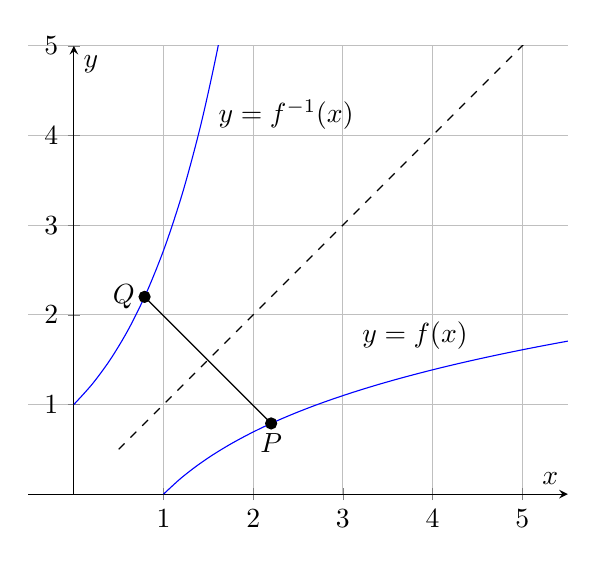
\begin{tikzpicture}
		\begin{axis}[
			xmin=0,xmax=5,
			ymin=0,ymax=5,
			restrict y to domain=0:10,
			grid=both,
			axis equal=true,
			axis lines=middle,
			xlabel=$x$,
			ylabel=$y$,
			axis lines=middle,
		]
			\begin{scope}[color=blue,samples=50,smooth]
				\addplot[domain=0:10]{exp(x)};
				\addplot[domain=1:10]{ln(x)};
			\end{scope}
			\addplot[color=black,dashed,domain=.5:8]{x};
			\filldraw(2.2,{ln(2.2)})circle(2pt)node[below]{$P$}
				--({ln(2.2)},2.2)circle(2pt)node[left]{$Q$};
			\draw(4.5,{ln(4.5)})node[above left]{$y=f(x)$}
				({ln(4.5)},4.5)node[below right]{$y=f^{-1}(x)$};
		\end{axis}
	\end{tikzpicture}
	\caption{}\label{figure:函数.直接函数与反函数的图形的对称性}
\end{figure}

\subsection{复合函数}
\begin{definition}
设函数\(y=f(u)\)的定义域为\(D_f\),
函数\(u=g(x)\)的定义域为\(D_g\),
且其值域\(R_g \subseteq D_f\),
则函数\[
	y = f[g(x)],
	\quad x \in D_g
\]
称为由函数\(u=g(x)\)与函数\(y=f(u)\)构成的\DefineConcept{复合函数},
它的定义域为\(D_g\),变量\(u\)称为\DefineConcept{中间变量}.

函数\(g\)与函数\(f\)构成的复合函数,
即按“先\(g\)后\(f\)”的次序复合的函数,
通常记为\(f \circ g\),即\[
	(f \circ g)(x) = f[g(x)].
\]
\end{definition}

\begin{proposition}
设\(f\)和\(g\)都是奇函数,
则\(f \circ g\)也是奇函数.
\begin{proof}
这是因为\(f[g(-x)]
= f[-g(x)]
= -f[g(x)]\).
\end{proof}
\end{proposition}

\begin{proposition}
设\(f\)和\(g\)都是偶函数,
则\(f \circ g\)也是偶函数.
\begin{proof}
这是因为\(f[g(-x)]
= f[g(x)]\).
\end{proof}
\end{proposition}

\begin{proposition}
设\(f\)是奇函数,\(g\)是偶函数,
则\(f \circ g\)和\(g \circ f\)都是偶函数.
\begin{proof}
这是因为\(f[g(-x)]
= f[g(x)]\),
\(g[f(-x)]
= g[-f(x)]
= g[f(x)]\).
\end{proof}
\end{proposition}

\begin{proposition}
设\(f\)和\(g\)是严格单调增加函数,
则\(f \circ g\)是严格单调增加函数.
\begin{proof}
对于\(\forall x_1,x_2 \in \dom(f \circ g)\),
当\(x_1 < x_2\)时,
有\(g(x_1) < g(x_2)\),
从而有\(f[g(x_1)] < f[g(x_2)]\),
这就说明\(f \circ g\)是严格单调增加函数.
\end{proof}
\end{proposition}

\begin{proposition}
设\(f\)和\(g\)是严格单调减少函数,
则\(f \circ g\)是严格单调增加函数.
\begin{proof}
对于\(\forall x_1,x_2 \in \dom(f \circ g)\),
当\(x_1 < x_2\)时,
有\(g(x_1) > g(x_2)\),
从而有\(f[g(x_1)] < f[g(x_2)]\),
这就说明\(f \circ g\)是严格单调增加函数.
\end{proof}
\end{proposition}

\begin{proposition}
设\(f\)是严格单调增加函数,
\(g\)是严格单调减少函数,
则\(f \circ g\)和\(g \circ f\)都是严格单调减少函数.
\begin{proof}
对于\(\forall x_1,x_2 \in \dom(f \circ g)\),
当\(x_1 < x_2\)时,
有\(g(x_1) > g(x_2)\),
从而有\(f[g(x_1)] > f[g(x_2)]\),
这就说明\(f \circ g\)是严格单调减少函数.
同理可证\(g \circ f\)也是严格单调减少函数.
\end{proof}
\end{proposition}

\section{绝对值函数}
\begin{definition}[绝对值]
设\(x \in \mathbb{R}\),则称函数\[
	f(x) = \left\{ \begin{array}{c}
		x, \quad x \geq 0 \\
		-x, \quad x < 0
	\end{array} \right.
\]为\(x\)的绝对值,
记作\(\abs{x}\).
\end{definition}

\begin{figure}[ht]
	\centering
	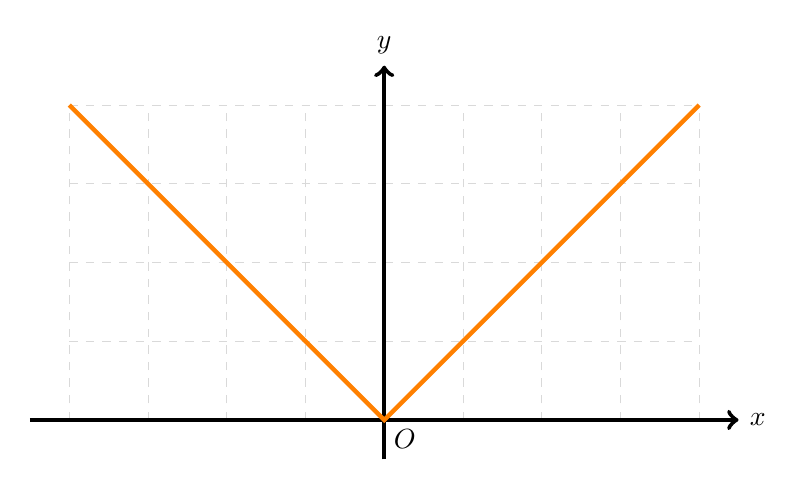
\begin{tikzpicture}
		\draw[help lines, color=gray!30, dashed] (-4,0) grid (4,4);
		\draw[->, ultra thick] (-4.5,0) -- (4.5,0) node[right]{\(x\)};
		\draw[->, ultra thick] (0,-0.5) -- (0,4.5) node[above]{\(y\)};
		\draw (0,0)node[below right]{\(O\)};
		\draw[orange,ultra thick] (-4,4)--(0,0)--(4,4);
	\end{tikzpicture}
	\caption{绝对值函数\(\abs{x}\)的图形}
\end{figure}

\begin{proposition}
设\(a,b\in\mathbb{R}\),
则\(\abs{ab} = \abs{a} \abs{b}\).
\begin{proof}
当\(a=0\)或\(b=0\)时,易见\(\abs{ab} = 0 = \abs{a} \abs{b}\).
当\(a\neq0\)且\(b\neq0\)时,
按照\(a\)和\(b\)的不同取值,列表如下:
\begin{center}
	\begin{tblr}{|*2c|*2{c|}}
		\hline
		&& \(b>0\) & \(b<0\) \\
		&& \(\abs{b}=b\) & \(\abs{b}=-b\) \\ \hline
		\(a>0\) & \(\abs{a}=a\) & \(ab>0,\abs{ab}=ab\) & \(ab<0,\abs{ab}=-ab\) \\ \hline
		\(a<0\) & \(\abs{a}=-a\) & \(ab<0,\abs{ab}=-ab\) & \(ab>0,\abs{ab}=ab\) \\ \hline
	\end{tblr}
\end{center}
由此可知\(\abs{ab} = \abs{a} \abs{b}\)恒成立.
\end{proof}
\end{proposition}

\begin{proposition}
设\(a\)和\(b\)都是实数,
则\begin{gather}
	\min\{a,b\}
	= \frac{a+b}{2}
	- \frac{\abs{a-b}}{2}, \\
	\max\{a,b\}
	= \frac{a+b}{2}
	+ \frac{\abs{a-b}}{2}.
\end{gather}
\begin{proof}
当\(a>b\)时,有\[
	\frac{a+b}{2} - \frac{\abs{a-b}}{2}
	= \frac{a+b}{2} - \frac{a-b}{2}
	= \frac{2b}{2} = b
	= \min\{a,b\},
\]\[
	\frac{a+b}{2} + \frac{\abs{a-b}}{2}
	= \frac{a+b}{2} + \frac{a-b}{2}
	= \frac{2a}{2} = a
	= \max\{a,b\}.
\]
当\(a \leq b\)时,有\[
	\frac{a+b}{2} - \frac{\abs{a-b}}{2}
	= \frac{a+b}{2} - \frac{b-a}{2}
	= \frac{2a}{2} = a
	= \min\{a,b\},
\]\[
	\frac{a+b}{2} + \frac{\abs{a-b}}{2}
	= \frac{a+b}{2} + \frac{b-a}{2}
	= \frac{2b}{2} = b
	= \max\{a,b\}.
	\qedhere
\]
\end{proof}
\end{proposition}

\section{符号函数}
\begin{definition}[符号函数]
函数\[
	f(x) = \left\{ \begin{array}{cc}
		1, & x > 0 \\
		0, & x = 0 \\
		-1, & x < 0 \\
	\end{array} \right.
\]称为\DefineConcept{符号函数},
记作\(\sgn x\).
\end{definition}

\begin{figure}[htb]
	\centering
	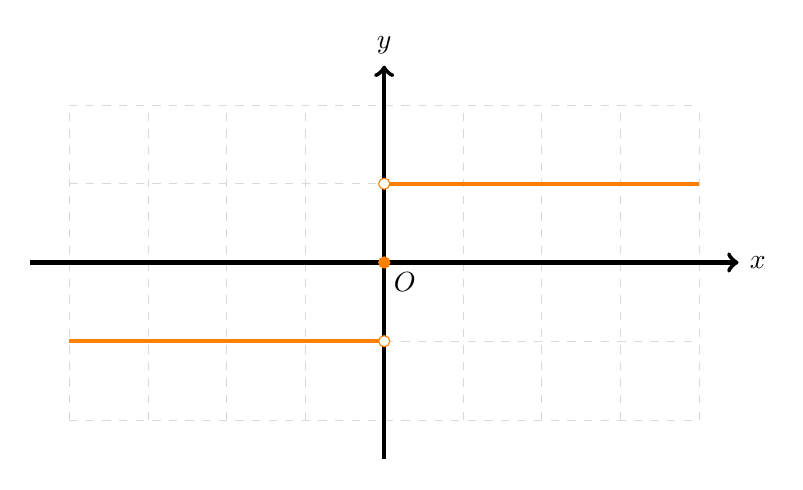
\begin{tikzpicture}
		\draw[help lines, color=gray!30, dashed] (-4,-2) grid (4,2);
		\draw[->, ultra thick] (-4.5,0) -- (4.5,0) node[right]{\(x\)};
		\draw[->, ultra thick] (0,-2.5) -- (0,2.5) node[above]{\(y\)};
		\draw (0,0)node[below right]{\(O\)};
		\draw[orange,ultra thick] (-4,-1)--(0,-1) (0,1)--(4,1);
		\draw[draw=orange,fill=orange] (0,0)circle(2pt);
		\draw[draw=orange,fill=white] (0,1)circle(2pt) (0,-1)circle(2pt);
	\end{tikzpicture}
	\caption{符号函数\(\sgn x\)的图形}
\end{figure}

\section{取整函数}
\begin{definition}[取整函数]
设\(x\in\mathbb{R},
n\in\mathbb{Z}\),定义:
\begin{enumerate}
	\item 如果\(n\)是不大于\(x\)的最大整数,
	即\(x\in[n,n+1)\),
	那么记\(\floor{x}=n\).
	我们把函数\(y=\floor{x}\)称为\DefineConcept{向下取整函数},
	即\begin{equation}
		\floor{x}
		\defeq
		\max\Set{ n\in\mathbb{Z} \given n \leq x }.
	\end{equation}

	\item 如果\(n\)是不小于\(x\)的最小整数,
	即\(x\in(n-1,n]\),
	那么记\(\ceil{x}=n\).
	我们把函数\(y=\ceil{x}\)称为\DefineConcept{向上取整函数},
	即\begin{equation}
		\ceil{x}
		\defeq
		\min\Set{ n\in\mathbb{Z} \given n \geq x }.
	\end{equation}
\end{enumerate}
\end{definition}

\begin{figure}[ht]
	\def\subwidth{.45\linewidth}
	\def\subscale{.9}
	\begin{subfigure}[b]{\subwidth}%
		\centering
		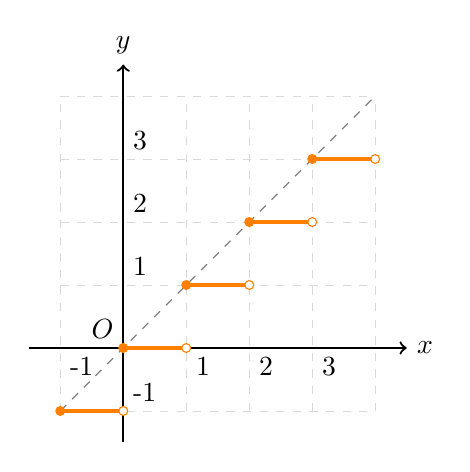
\begin{tikzpicture}[scale=\subscale]
			\tikzstyle{sx}=[draw=orange,fill=orange]
			\tikzstyle{kx}=[draw=orange,fill=white]
			\draw[help lines, color=gray!30, dashed] (-1,-1) grid (4,4);
			\draw[dashed, color=gray] (-1,-1) -- (4,4);
			\draw[->, thick] (-1.5,0) -- (4.5,0) node[right]{\(x\)};
			\draw[->, thick] (0,-1.5) -- (0,4.5) node[above]{\(y\)};
			\foreach \i in {-1,...,3} {
				\draw[ultra thick,orange] (\i,\i)--(\i+1,\i);
				\fill[sx] (\i,\i)circle(2pt);
				\fill[kx] (\i+1,\i)circle(2pt);
				\ifnum\i=0\relax\else
					\draw(\i,0)node[below right]{\i};
					\draw(0,\i)node[above right]{\i};
				\fi
			}
			\draw (0,0)node[above left]{\(O\)};
		\end{tikzpicture}
		\subcaption{向下取整函数\(\floor{x}\)}
	\end{subfigure}
	\begin{subfigure}[b]{\subwidth}%
		\centering
		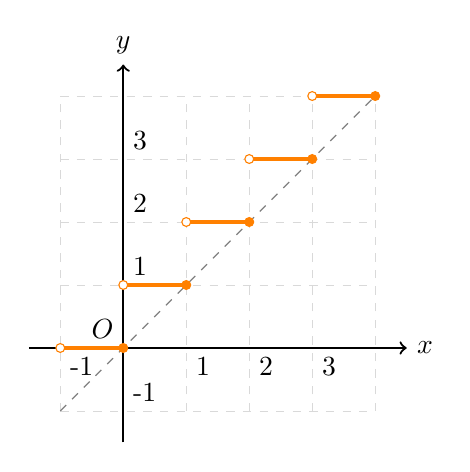
\begin{tikzpicture}[scale=\subscale]
			\tikzstyle{sx}=[draw=orange,fill=orange]
			\tikzstyle{kx}=[draw=orange,fill=white]
			\draw[help lines, color=gray!30, dashed] (-1,-1) grid (4,4);
			\draw[dashed, color=gray] (-1,-1) -- (4,4);
			\draw[->, thick] (-1.5,0) -- (4.5,0) node[right]{\(x\)};
			\draw[->, thick] (0,-1.5) -- (0,4.5) node[above]{\(y\)};
			\foreach \i in {-1,...,3} {
				\draw[ultra thick,orange] (\i,\i+1)--(\i+1,\i+1);
				\fill[kx] (\i,\i+1)circle(2pt);
				\fill[sx] (\i+1,\i+1)circle(2pt);
				\ifnum\i=0\relax\else
					\draw(\i,0)node[below right]{\i};
					\draw(0,\i)node[above right]{\i};
				\fi
			}
			\draw (0,0)node[above left]{\(O\)};
		\end{tikzpicture}
		\subcaption{向上取整函数\(\ceil{x}\)}
	\end{subfigure}
	\caption{取整函数的图形}
\end{figure}

\begin{property}\label{theorem:取整函数.性质1}
一般地,对于\(x\in\mathbb{R}\),总有\begin{equation}
	x - 1 < \floor{x} \leq x \leq \ceil{x} < x + 1.
\end{equation}
\end{property}

\begin{property}
对于\(n\in\mathbb{Z}\),总有\begin{equation}
	\ceil{n/2} + \floor{n/2} = n.
\end{equation}
\end{property}

\begin{property}
对于任意实数\(x \geq 0\)和整数\(a,b>0\),总有\begin{gather}
	\ceil*{\frac{\ceil{x/a}}{b}} = \ceil*{\frac{x}{ab}}, \\
	\floor*{\frac{\floor{x/a}}{b}} = \floor*{\frac{x}{ab}}, \\
	\ceil*{\frac{a}{b}} \leq \frac{a+(b-1)}{b}, \\
	\floor*{\frac{a}{b}} \geq \frac{a-(b-1)}{b}.
\end{gather}
\end{property}

\section{幂函数、指数函数、对数函数}
\begin{definition}
同一个数\(a\ (a\in\mathbb{R})\)连续相乘\(b\ (b\in\mathbb{N})\)次所得的乘积,
称作“\(a\)的\(b\)次方”
或“\(a\)的\(b\)次幂”,
记作\(a^b\),
即\[
	a^b
	\defeq
	\underbrace{a \times a \times \dotsm \times a}_{b\text{次}} = \prod_{i=1}^b a.
\]

特别地,规定:\begin{gather*}
	a^0 \defeq 1 \quad(a\neq0), \\
	a^{-1} \defeq \frac1a \quad(a\neq0), \\
	a^{-n} \defeq \frac1{a^n} \quad(a\neq0), \\
	a^{1/n} \defeq \sqrt[n]{a} \quad(a\geq0). \\
\end{gather*}
\end{definition}

\begin{figure}[ht]
	\centering
	\begin{tikzpicture}
		\def\r{\textcolor{orange}}
		\def\b{\textcolor{blue}}
		\def\p{\textcolor{purple}}
		\draw(0,0)node{\(\r{a}^{\b{b}} = \p{c} \defiff \log_{\r{a}} \p{c} = \b{b}\)};
		\draw(-2.2,-.5)node{\r{底数}}
			(-2.2,.5)node{\b{指数}}
			(-1,-.5)node{\p{幂}}
			(.3,-.5)node{\r{底数}}
			(1.4,-.5)node{\p{真数}}
			(2.3,.5)node{\b{对数}};
		\draw[->](-1.7,-.3)--(-1.7,-1)--(.84,-1)->(.84,-.3); %a
		\draw[->](-1.55,.3)--(-1.55,1)--(1.7,1)->(1.7,.3); %b
		\draw[->](-.86,.3)--(-.86,.7)--(1.1,.7)->(1.1,.3); %c
	\end{tikzpicture}
	\caption{底数、指数、幂与对数的联系}\label{figure:函数.底数、指数、幂与对数的联系}
\end{figure}

\begin{proposition}
\(1\)的任意次幂还是\(1\),即\(1^n = 1\).
\end{proposition}

\begin{proposition}
\(0\)的任意非零次幂还是\(0\),即\(0^n = 0\ (n\neq0)\).
\end{proposition}

\subsection{幂函数的概念}
\begin{definition}[幂函数]
函数\(f(x)=x^{\mu}\ (\mu \in \mathbb{R})\),
称为\DefineConcept{幂函数}.
\end{definition}

\subsection{幂函数的性质}
\begin{property}
幂函数具有以下性质:
\begin{itemize}
	\item 当\(\mu = 0\)时,
	幂函数\(f(x)=x^{\mu}\)在定义域\((-\infty,+\infty)\)上恒为一,
	是常数函数.

	\item 当\(\mu\)为正奇数时,
	幂函数\(f(x)=x^{\mu}\)为奇函数,
	其定义域、值域均为\((-\infty,+\infty)\),它在定义域内恒单调递增.

	\item 当\(\mu\)为正偶数时,
	幂函数\(f(x)=x^{\mu}\)为偶函数,
	其定义域为\((-\infty,+\infty)\),其值域为\([0,+\infty)\),
	它在\((-\infty,0]\)上单调递减,在\([0,+\infty)\)上单调递增.

	\item 当\(\mu\)为负奇数时,
	幂级数\(y=x^{\mu}\)又称为\DefineConcept{比例函数},
	其定义域、值域为\((-\infty,0)\cup(0,+\infty)\),
	它在区间\((-\infty,0)\)和\((0,+\infty)\)内单调递减.

	若幂函数前有常系数大于零则称之为\DefineConcept{正比例函数}.
	%@Mathematica: Plot[Evaluate[x^-n /. n -> {1, 2, 3, 4, 5}], {x, 0, 2}, PlotRange -> {0, 2}, PlotLegends -> Automatic]

	若幂函数前有常系数小于零则称之为\DefineConcept{反比例函数}.
	%@Mathematica: Plot[Evaluate[x^-n /. n -> {1, 2, 3, 4, 5}], {x, -2, 0}, PlotRange -> {-2, 2}, PlotLegends -> Automatic]

	\item 当\(\mu\)为负偶数时,
	幂函数\(f(x)=x^{\mu}\)为偶函数,
	其定义域为\((-\infty,0)\cup(0,+\infty)\),其值域为\((0,+\infty)\),
	它在\((-\infty,0)\)内单调递增,在\((0,+\infty)\)内单调递减.

	\item 当\(\mu = \pm\frac{m}{n} \in \mathbb{Q}\)(\(m,n>0\)且\(m\)、\(n\)是互质的整数)时,
	幂函数\(f(x)=x^{\mu}=x^{\pm\frac{m}{n}}\)可改写为\(y=\sqrt[n]{x^m}\)(\(\mu>0\)时)
	或\(y=\frac{1}{\sqrt[n]{x^m}}\)(\(\mu<0\)时).
\end{itemize}
\end{property}

\begin{figure}[ht]
	\centering
	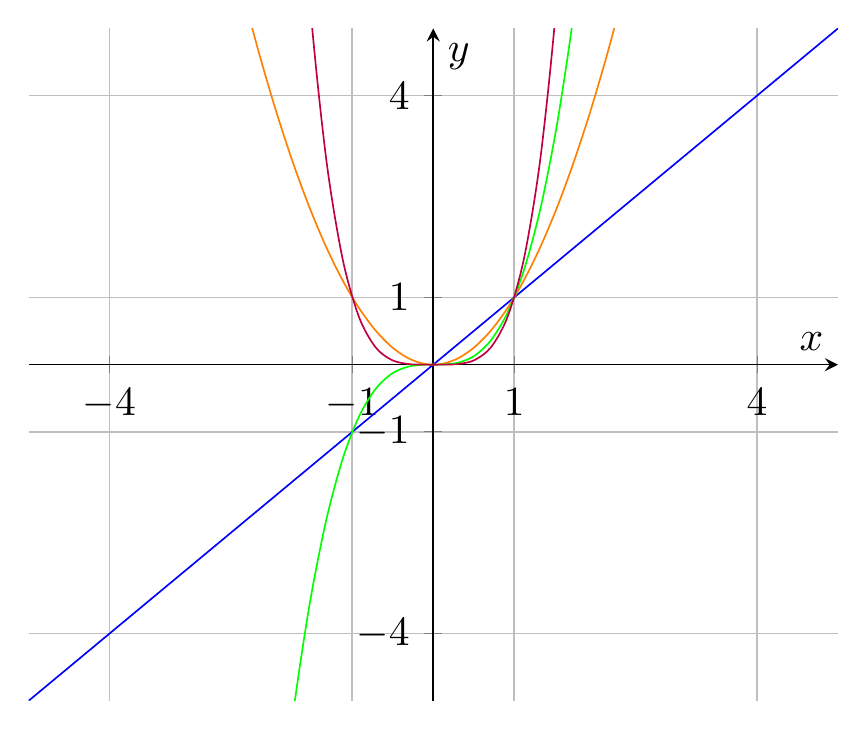
\begin{tikzpicture}[scale=1.5]
		\begin{axis}[
			xmin=-5,xmax=5,
			ymin=-5,ymax=5,
			enlargelimits,
			axis lines=middle,
			xlabel=$x$,
			ylabel=$y$,
			xtick={-4,-1,1,4},
			ytick={-4,-1,1,4},
			grid=major,
		]
			\begin{scope}[samples=50,smooth,domain=-5:5]
				\addplot[color=blue]{x};
				\addplot[color=orange]{x^2};
				\addplot[color=green]{x^3};
				\addplot[color=purple]{x^4};
			\end{scope}
		\end{axis}
	\end{tikzpicture}
	\caption{}
\end{figure}

\begin{figure}
	\centering
	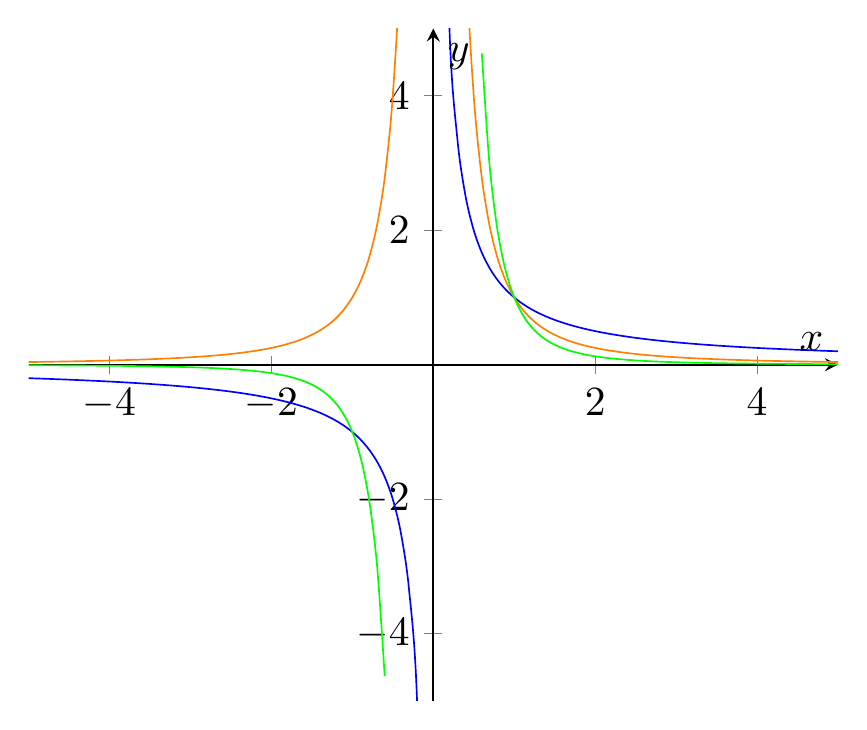
\begin{tikzpicture}[scale=1.5]
		\begin{axis}[
			xmin=-5,xmax=5,
			ymin=-5,ymax=5,
			enlargelimits,
			axis lines=middle,
			xlabel=$x$,
			ylabel=$y$,
		]
			\begin{scope}[samples=50,smooth]
				\begin{scope}[domain=-5:-.1]
					\addplot[color=blue]{1/x};
					\addplot[color=orange]{1/(x^2)};
					\addplot[color=green,domain=-5:-.6]{1/(x^3)};
				\end{scope}
				\begin{scope}[domain=.1:5]
					\addplot[color=blue]{1/x};
					\addplot[color=orange]{1/(x^2)};
					\addplot[color=green,domain=.6:5]{1/(x^3)};
				\end{scope}
			\end{scope}
		\end{axis}
	\end{tikzpicture}
	\caption{}
\end{figure}

\subsection{指数函数的概念}
\begin{definition}
设\(a>0\)且\(a \neq 1\).
把函数\(f(x)=a^x\)
称为“以\(a\)为底的\DefineConcept{指数函数}”.
\end{definition}

\begin{theorem}
设\(f\)是以\(a\)为底的指数函数,
则\(f\)存在反函数.
\begin{proof}
指数函数是单调函数.
\end{proof}
\end{theorem}

\subsection{指数函数的性质}
\begin{property}
\begin{gather}
	a^x a^y = a^{x+y}, \\
	\frac{a^x}{a^y} = a^{x-y}, \\
	(a^x)^y = a^{xy}.
\end{gather}
\end{property}

\subsection{对数函数的概念}
\begin{definition}
设\(a>0\)且\(a\neq1\).
以\(a\)为底的指数函数的反函数,
称为“以\(a\)为底的\DefineConcept{对数函数}”,
记作\(\log_a x\),
即\begin{equation}\label{equation:函数.对数的定义}
	y = \log_a x
	\defiff
	a^y = x.
\end{equation}
%@see: https://mathworld.wolfram.com/Logarithm.html
\end{definition}

以\(10\)为底的对数,称为\DefineConcept{常用对数},记作\(y = \lg x\),
即\begin{equation}
	\lg x \defeq \log_{10} x.
\end{equation}

以常数\(e\)为底的对数,称为\DefineConcept{自然对数},记作\(y = \ln x\),
即\begin{equation}
	\ln x \defeq \log_e x.
\end{equation}

\subsection{对数函数的性质}
\begin{proposition}[对数恒等式]
设\(a>0,a\neq1\),
则对\(\forall x>0\)
有\begin{equation}\label{equation:函数.对数恒等式}
	a^{\log_a x} = x.
\end{equation}
\begin{proof}
根据\hyperref[equation:函数.对数的定义]{对数的定义}有
\(y = \log_a x
\defiff
a^y = x\),
于是\(a^{\log_a x} = a^y = x\).
\end{proof}
\end{proposition}

\begin{theorem}
设\(a>0,a\neq1\),
则\begin{gather}
	\log_a 1 = 0, \\
	\log_a a = 1.
\end{gather}
\end{theorem}

\begin{theorem}[对数的运算法则]
设\(a>0,a\neq1,x>0,y>0\),
则\begin{gather}
	\log_a xy = \log_a x + \log_a y,
		\label{equation:函数.对数的基本运算法则1} \\
	\log_a \frac{x}{y} = \log_a x - \log_a y,
		\label{equation:函数.对数的基本运算法则2} \\
	\log_a x^y = y \log_a x.
		\label{equation:函数.对数的基本运算法则3}
\end{gather}
\end{theorem}

\begin{theorem}[换底公式]
设\(a>0,a\neq1,c>0,c\neq1,b>0\),
则\begin{equation}\label{equation:函数.换底公式}
	\log_a b = \frac{\log_c b}{\log_c a}.
\end{equation}
\begin{proof}
由\hyperref[equation:函数.对数恒等式]{对数恒等式}有\(b = a^{\log_a b}\),
于是\(\log_c b
= \log_c a^{\log_a b}\).
又由有\hyperref[equation:函数.对数的基本运算法则3]{对数的运算法则}有\[
	\log_c a^{\log_a b} = \log_a b \cdot \log_c a,
\]
所以\(\log_a b = \frac{\log_c b}{\log_c a}\).
\end{proof}
\end{theorem}

\begin{corollary}
设\(a>0,a\neq1,b>0,b\neq1\),
则\begin{equation}
	\log_a b = \frac1{\log_b a}.
\end{equation}
\begin{proof}
在\hyperref[equation:函数.换底公式]{换底公式}中,令\(c=b\)便得.
\end{proof}
\end{corollary}

\begin{corollary}
设\(a>0,a\neq1,a^x\neq1\)
则\begin{equation}
	\log_{a^x} b^y = \frac{y}{x} \log_a b.
\end{equation}
\end{corollary}

\begin{example}
设\(a>0,b>0\).
证明:\begin{equation}\label{equation:函数.真底互换公式}
	a^{\ln b} = b^{\ln a}.
\end{equation}
\begin{proof}
在\cref{equation:函数.真底互换公式} 等号左右变量分别取对数,
得\[
	\ln(a^{\ln b}) = \ln b \ln a, \qquad
	\ln(b^{\ln a}) = \ln a \ln b,
\]
显然两者相等,故\(a^{\ln b} = b^{\ln a}\)成立.
\end{proof}
\end{example}

\subsection{重幂}
设\(a\)是实数,\(b\)是正整数.
定义:\[
	\relax^ba \defeq \underbrace{a^{a^{\iddots^a}}}_{\text{\(b\)个}},
\]
我们把\(\relax^ba\)读作“\(a\)的\(b\)~\DefineConcept{重幂}”.

例如,\[
	\relax^23 = 3^3, \qquad
	\relax^33 = 3^{3^3}, \qquad
	\relax^43 = 3^{3^{3^3}}.
\]

\section{三角函数}
\subsection{三角函数的概念}
\begin{figure}[htb]
	\centering
	\begin{tikzpicture}[scale=6]
		\draw(1,0)coordinate(A)node[below]{$A$}
			arc[start angle=0,end angle=90,radius=1](0,1)node[left]{$B$};
		\draw(0,0)coordinate(O)node[below left]{$O$}
			--(.866,.5)coordinate(P)node[above]{$P$}
			--(.866,0)coordinate(Q)node[below]{$Q$};
		\draw(P)--(1,.577)coordinate(R)node[right]{$R$}--(A);
		\begin{scope}[->,>=Stealth]
			\draw(0,0)--(1.2,0)node[below]{$x$};
			\draw(0,0)--(0,1.2)node[left]{$y$};
		\end{scope}
		\draw pic["$\theta$",draw=orange,-,angle eccentricity=1.2,angle radius=1cm]{angle=Q--O--P};
		\draw pic[draw=gray,-,angle radius=.5cm]{right angle=P--Q--O};
	\end{tikzpicture}
	\caption{}
	\label{figure:函数.三角函数.三角函数的几何定义}
\end{figure}

如\cref{figure:函数.三角函数.三角函数的几何定义},
首先在平面直角坐标系\(Oxy\)中
画出一个单位圆\(\odot~O\),
分别交\(x\)轴、\(y\)轴于\(A\)、\(B\)两点.
在\(\odot~O\)上任取一点\(P\),过\(P\)作\(OA\)的垂线交\(OA\)于\(Q\).
过点\(A\)作\(OA\)的垂线交射线\(OP\)于\(R\).
记\(\angle POQ = \theta\).
定义:\begin{gather}
	\sin\theta \defeq \abs{\overline{PQ}}, \\
	\cos\theta \defeq \abs{\overline{OQ}}, \\
	\tan\theta \defeq \sin\theta/\cos\theta, \\
	\cot\theta \defeq \cos\theta/\sin\theta, \\
	\sec\theta \defeq 1/\cos\theta, \\
	\csc\theta \defeq 1/\sin\theta.
\end{gather}
我们把\(\sin,\cos,\tan,\cot,\sec,\csc\)
依次称为\DefineConcept{正弦函数}、
\DefineConcept{余弦函数}、
\DefineConcept{正切函数}、
\DefineConcept{余切函数}、
\DefineConcept{正割函数}、
\DefineConcept{余割函数},
统称为\DefineConcept{三角函数}.

不难想象,当\(P\)在圆周上逆时针平移时,
\(\theta\)逐渐增大,
线段\(\overline{OP}\)的长度\(\abs{\overline{OP}}\)始终保持不变,
线段\(\overline{PQ}\)的长度\(\abs{\overline{PQ}}\)逐渐增大,
线段\(\overline{OQ}\)的长度\(\abs{\overline{OQ}}\)逐渐减小.
当\(P\)与\(B\)重合时,
\(\abs{\overline{OP}}
= \abs{\overline{PQ}}
= \abs{\overline{OB}} = 1\)
且\(\abs{\overline{OQ}} = 0\).
当\(P\)在圆周上顺时针平移时,
\(\theta\)逐渐减小,
线段\(\overline{OP}\)的长度\(\abs{\overline{OP}}\)依旧始终保持不变,
线段\(\overline{PQ}\)的长度\(\abs{\overline{PQ}}\)逐渐减小,
线段\(\overline{OQ}\)的长度\(\abs{\overline{OQ}}\)逐渐增大.
当\(P\)与\(A\)重合时,
\(\abs{\overline{OP}}
= \abs{\overline{OA}} = 1\)
且\(\abs{\overline{PQ}} = 0\).

\begin{example}
下面列出一些特殊的正弦函数值:\[
	\sin0 = 0, \quad
	\sin\frac{\pi}{6} = \frac{1}{2}, \quad
	\sin\frac{\pi}{4} = \frac{\sqrt{2}}{2}, \quad
	\sin\frac{\pi}{3} = \frac{\sqrt{3}}{2},
\]\[
	\sin\frac{\pi}{2} = 1, \quad
	\sin\pi = 0, \quad
	\sin\frac{3\pi}{2} = -1.
\]

\begin{figure}[htb]
	\centering
	\begin{tikzpicture}
		\pgfmathsetmacro{\r}{2}
		\pgfmathsetmacro{\ax}{\r*cos(30)}
		\pgfmathsetmacro{\ay}{\r*sin(30)}
		\pgfmathsetmacro{\b}{\r/sqrt(2)}
		\coordinate (O)at(0,0);
		\draw(O)circle(\r);
		\begin{scope}[dashed,color=gray!50,text=black]
			\draw(O)--(\r,0)node[left]{\(0\)}node[right]{\(0\)}
			(O)--(\ax,\ay)node[below left]{\(\tfrac{\pi}{6}\)}node[right]{\(\tfrac{1}{2}\)}
			(O)--(\b,\b)node[below left]{\(\tfrac{\pi}{4}\)}node[above right]{\(\tfrac{\sqrt2}{2}\)}
			(O)--(\ay,\ax)node[below left]{\(\tfrac{\pi}{3}\)}node[above]{\(\tfrac{\sqrt3}{2}\)}
			(O)--(0,\r)node[below]{\(\tfrac{\pi}{2}\)}node[above]{\(1\)}
			(O)--(-\ay,\ax)node[below right]{\(\tfrac{2\pi}{3}\)}node[above]{\(\tfrac{\sqrt3}{2}\)}
			(O)--(-\b,\b)node[below right]{\(\tfrac{3\pi}{4}\)}node[above left]{\(\tfrac{\sqrt2}{2}\)}
			(O)--(-\ax,\ay)node[below right]{\(\tfrac{5\pi}{6}\)}node[left]{\(\tfrac{1}{2}\)}
			(O)--(-\r,0)node[right]{\(\pi\)}node[left]{\(0\)}
			(O)--(-\ax,-\ay)node[above right]{\(\tfrac{7\pi}{6}\)}node[left]{\(-\tfrac{1}{2}\)}
			(O)--(-\b,-\b)node[above right]{\(\tfrac{5\pi}{4}\)}node[below left]{\(-\tfrac{\sqrt2}{2}\)}
			(O)--(-\ay,-\ax)node[above right]{\(\tfrac{4\pi}{3}\)}node[below]{\(-\tfrac{\sqrt3}{2}\)}
			(O)--(0,-\r)node[above]{\(\tfrac{3\pi}{2}\)}node[below]{\(-1\)}
			(O)--(\ay,-\ax)node[above left]{\(\tfrac{5\pi}{3}\)}node[below]{\(-\tfrac{\sqrt3}{2}\)}
			(O)--(\b,-\b)node[above left]{\(\tfrac{7\pi}{4}\)}node[below right]{\(-\tfrac{\sqrt2}{2}\)}
			(O)--(\ax,-\ay)node[above left]{\(\tfrac{11\pi}{6}\)}node[right]{\(-\tfrac{1}{2}\)}
			;
		\end{scope}
		\begin{scope}[very thick,->]
			\draw(-1,0)--(1,0)node[above left]{\(x\)};
			\draw(0,-1)--(0,1)node[below right]{\(y\)};
		\end{scope}
	\end{tikzpicture}
	\caption{正弦函数\(\sin x\)的辅助圆与特殊值}
\end{figure}

特殊的余弦函数值:\[
	\cos0 = 1, \quad
	\cos\frac{\pi}{6} = \frac{\sqrt{3}}{2}, \quad
	\cos\frac{\pi}{4} = \frac{\sqrt{2}}{2}, \quad
	\cos\frac{\pi}{3} = \frac{1}{2},
\]\[
	\cos\frac{\pi}{2} = 0, \quad
	\cos\pi = -1, \quad
	\cos\frac{3\pi}{2} = 0.
\]
\end{example}

\subsection{三角函数的性质}
\begin{property}
根据三角函数的定义,显然有\begin{gather}
	\tan\theta = \frac{\sin\theta}{\cos\theta},
	\label{equation:三角函数.正切与正余弦的关系} \\
	\cot\theta = \frac{1}{\tan\theta}, \\
	\sec\theta = \frac{1}{\cos\theta}, \\
	\csc\theta = \frac{1}{\sin\theta}.
\end{gather}
\end{property}

\begin{theorem}[毕达哥拉斯三角恒等式]
\begin{figure}[htb]
	\def\subwidth{.5\linewidth}
	\def\subscale{.8}
		\begin{subfigure}[b]{\subwidth}%
		\centering
		\begin{tikzpicture}[scale=\subscale]
			\draw[help lines, color=gray!30, dashed] (0,0) grid (4,3);
			\coordinate (A) at (0,0);
			\coordinate (B) at (4,0);
			\coordinate (C) at (4,3);
			\draw (A)node[left]{\(A\)} -- (B)node[right]{\(B\)}node[midway,below]{\(\cos\theta\)} -- (C)node[right]{\(C\)}node[midway,right]{\(\sin\theta\)} -- (A)node[midway,above left]{\(1\)} pic["\(\theta\)",draw=orange,-,angle eccentricity=2,angle radius=0.3cm]{angle=B--A--C} pic[draw=gray,-,angle radius=0.3cm]{right angle=C--B--A};
		\end{tikzpicture}
		\subcaption{正弦、余弦辅助三角形}
		\end{subfigure}%
		\begin{subfigure}[b]{\subwidth}%
		\centering
		\begin{tikzpicture}[scale=\subscale]
			\draw[help lines, color=gray!30, dashed] (0,0) grid (4,3);
			\coordinate (A) at (0,0);
			\coordinate (B) at (4,0);
			\coordinate (C) at (4,3);
			\draw (A)node[left]{\(A\)} -- (B)node[right]{\(B\)}node[midway,below]{\(1\)} -- (C)node[right]{\(C\)}node[midway,right]{\(\tan\theta\)} -- (A)node[midway,above left]{\(\sec\theta\)} pic["\(\theta\)",draw=orange,-,angle eccentricity=2,angle radius=0.3cm]{angle=B--A--C} pic[draw=gray,-,angle radius=0.3cm]{right angle=C--B--A};
		\end{tikzpicture}
		\subcaption{正切、正割辅助三角形}
		\end{subfigure}%
	\caption{两种特殊的辅助三角形}
	\label{figure:函数.两种特殊的辅助三角形}
\end{figure}

结合\cref{figure:函数.两种特殊的辅助三角形},根据勾股定理可得
\begin{gather}
	\sin^2 \theta + \cos^2 \theta = 1,
		\label{equation:三角函数.毕达哥拉斯三角恒等式1} \\
	\tan^2 \theta + 1 = \sec^2 \theta, \\
	1 + \cot^2 \theta = \csc^2 \theta.
\end{gather}
\end{theorem}

\begin{figure}[htb]
	\centering
	\begin{tikzpicture}
		\pgfmathsetmacro{\a}{6}
		\coordinate(O)at(0,0);
		\pgfmathsetmacro{\t}{30}
		\draw(O)node[below left]{\(O\)}
			--(\a,0)coordinate(A)node[below right]{\(A\)}
			arc[start angle=0,end angle=\t,radius=\a]coordinate(B)node[right]{\(B\)}
			--(O);
		\draw(B)--(B|-A)coordinate(C)node[below right]{\(C\)};
		\draw(B)--(\a,{\a*tan(\t)})coordinate(D)node[above right]{\(D\)}--(\a,0);
		\pic["\(\theta\)",draw,-,angle eccentricity=1.5,angle radius=6mm]{angle=A--O--B};
		\begin{scope}[|<->|,black!40,every node/.style={black,midway,sloped}]
			\def\mark#1#2#3#4#5{%
				\draw($#1+#4$)--($#2+#4$)node[#3]{$#5$};%
			}%
			\mark{(C)}{(B)}{above}{(-5pt,0)}{\sin\theta}
			\mark{(O)}{(D)}{above}{({(-1em-10pt)*sin(30)},{(1em+10pt)*cos(30)})}{\sec\theta}
			\mark{(O)}{(B)}{above}{({-5pt*sin(30)},{5pt*cos(30)})}{1}
			\mark{(O)}{(C)}{below}{(0,-5pt)}{\cos\theta}
			\mark{(A)}{(D)}{below}{(5pt,0)}{\tan\theta}
			\mark{(O)}{(A)}{below}{(0,-1em-10pt)}{1}
		\end{scope}
	\end{tikzpicture}
	\caption{}
\end{figure}

\begin{figure}[htb]
	\centering
	\begin{tikzpicture}[scale=.5]
		\begin{axis}[
			xmin=-10,xmax=10,
			restrict y to domain=-2:2,
			ymin=-1,ymax=1,
			grid=both,width=\textwidth,height=\textwidth,
			axis lines=middle,
			xlabel=$x$,
			ylabel=$y$,
			enlarge x limits=0.1,
			enlarge y limits=0.1,
			x label style={at={(ticklabel* cs:1.00)}, inner sep=5pt, anchor=west},
			y label style={at={(ticklabel* cs:1.00)}, inner sep=2pt, anchor=south},
		]
			\addplot[color=blue,samples=50,smooth,domain=-10:10,variable=\x]{sin(\x r)};
		\end{axis}
	\end{tikzpicture}
	\caption{正弦函数\(y=\sin x\)的图形}
	\label{figure:函数.正弦函数的图形}
\end{figure}

\begin{figure}
	\centering
	\begin{tikzpicture}[scale=.5]
		\begin{axis}[
			name=Sine,
			xmin=0,xmax=10,
			restrict y to domain=-2:2,
			ymin=-1,ymax=1,
			grid=both,width=\textwidth,height=\textwidth,
			axis lines=middle,
			xlabel=$x$,
			ylabel=$y$,
			x label style={at={(ticklabel* cs:1.00)}, inner sep=5pt, anchor=west},
			y label style={at={(ticklabel* cs:1.00)}, inner sep=2pt, anchor=south},
			xtick={0,1.5708,3.1416,...,10},
			xticklabels={
				$\relax$,
				$\frac{\pi}{2}$,
				$\pi\vphantom{\frac12}$,
				$\frac{3\pi}{2}$,
				$2\pi\vphantom{\frac12}$,
				$\frac{5\pi}{2}$,
				$3\pi\vphantom{\frac12}$,
			},
		]
			\addplot[color=blue,samples=50,smooth,domain=0:10,variable=\x]
				{sin(.5*\x r)};\label{pgfplots:正弦函数.sin(x/2)}
			\addplot[color=orange,samples=50,smooth,domain=0:10,variable=\x]
				{sin(\x r)};\label{pgfplots:正弦函数.sin(x)}
			\addplot[color=green,samples=50,smooth,domain=0:10,variable=\x]
				{sin(2*\x r)};\label{pgfplots:正弦函数.sin(2*x)}
		\end{axis}
		\node[draw,fill=white,inner sep=0pt,right=1em]at(Sine.east){\small\begin{tabular}{cl}
		\ref{pgfplots:正弦函数.sin(x/2)} & \(\sin(x/2)\) \\
		\ref{pgfplots:正弦函数.sin(x)} & \(\sin x\) \\
		\ref{pgfplots:正弦函数.sin(2*x)} & \(\sin2x\) \\
		\end{tabular}};
	\end{tikzpicture}
	\caption{}
\end{figure}

\begin{property}
如\cref{figure:函数.正弦函数的图形},
可以观察得出正弦函数的若干性质.
\begin{enumerate}
	\item 正弦函数是周期函数,其周期为\(T = 2\pi\).
	\item 正弦函数在区间\([2k\pi-\frac{\pi}{2},2k\pi+\frac{\pi}{2})\)上单调递增.
	\item 在区间\([2k\pi+\frac{\pi}{2},2k\pi+\frac{3\pi}{2})\)上单调递增.
	\item 当\(x=\frac{\pi}{2}+2k\pi\ (k\in\mathbb{Z})\)时,正弦函数\(y=\sin x\)取得极大值\(1\).
	\item 当\(x=\frac{3\pi}{2}+2k\pi\ (k\in\mathbb{Z})\)时,正弦函数\(y=\sin x\)取得极小值\(-1\).
	\item 正弦函数是奇函数,其图形关于坐标原点\(O\)中心对称,满足\(\sin(-x)=-\sin x\).
\end{enumerate}
\end{property}

\begin{figure}[htb]
	\centering
	\begin{tikzpicture}[scale=.5]
		\begin{axis}[
			xmin=-10,xmax=10,
			restrict y to domain=-2:2,
			ymin=-1,ymax=1,
			grid=both,width=\textwidth,height=\textwidth,
			axis lines=middle,
			xlabel=$x$,
			ylabel=$y$,
			enlarge x limits=0.1,
			enlarge y limits=0.1,
			x label style={at={(ticklabel* cs:1.00)}, inner sep=5pt, anchor=west},
			y label style={at={(ticklabel* cs:1.00)}, inner sep=2pt, anchor=south},
		]
			\addplot[color=blue,samples=50,smooth,domain=-10:10,variable=\x]{cos(\x r)};
		\end{axis}
	\end{tikzpicture}
	\caption{余弦函数\(y=\cos x\)的图形}
	\label{figure:函数.余弦函数的图形}
\end{figure}

\begin{figure}
	\centering
	\begin{tikzpicture}[scale=.5]
		\begin{axis}[
			name=Cosine,
			xmin=0,xmax=10,
			restrict y to domain=-2:2,
			ymin=-1,ymax=1,
			grid=both,width=\textwidth,height=\textwidth,
			axis lines=middle,
			xlabel=$x$,
			ylabel=$y$,
			x label style={at={(ticklabel* cs:1.00)}, inner sep=5pt, anchor=west},
			y label style={at={(ticklabel* cs:1.00)}, inner sep=2pt, anchor=south},
			xtick={0,1.5708,3.1416,...,10},
			xticklabels={
				$\relax$,
				$\frac{\pi}{2}$,
				$\pi\vphantom{\frac12}$,
				$\frac{3\pi}{2}$,
				$2\pi\vphantom{\frac12}$,
				$\frac{5\pi}{2}$,
				$3\pi\vphantom{\frac12}$,
			},
		]
			\addplot[color=blue,samples=50,smooth,domain=0:10,variable=\x]
				{cos(.5*\x r)};\label{pgfplots:余弦函数.cos(x/2)}
			\addplot[color=orange,samples=50,smooth,domain=0:10,variable=\x]
				{cos(\x r)};\label{pgfplots:余弦函数.cos(x)}
			\addplot[color=green,samples=50,smooth,domain=0:10,variable=\x]
				{cos(2*\x r)};\label{pgfplots:余弦函数.cos(2*x)}
		\end{axis}
		\node[draw,fill=white,inner sep=0pt,right=1em]at(Cosine.east){\small\begin{tabular}{cl}
		\ref{pgfplots:余弦函数.cos(x/2)} & \(\cos(x/2)\) \\
		\ref{pgfplots:余弦函数.cos(x)} & \(\cos x\) \\
		\ref{pgfplots:余弦函数.cos(2*x)} & \(\cos2x\) \\
		\end{tabular}};
	\end{tikzpicture}
	\caption{}
\end{figure}

\begin{property}
如\cref{figure:函数.余弦函数的图形},
可以观察得出余弦函数的若干性质.
\begin{enumerate}
	\item 余弦函数也是周期函数,其周期为\(T = 2\pi\).
	\item 余弦函数在区间\([2k\pi,\pi+2k\pi)\)上单调递减.
	\item 在区间\([\pi+2k\pi,2\pi+2k\pi)\)上单调递增.
	\item 当\(x=2k\pi\ (k\in\mathbb{Z})\)时,余弦函数\(y=\cos x\)取得极大值\(1\).
	\item 当\(x=(2k-1)\pi\ (k\in\mathbb{Z})\)时,余弦函数\(y=\cos x\)取得极小值\(-1\).
	\item 余弦函数是偶函数,其图形关于\(y\)轴对称,满足\(\cos(-x)=\cos x\).
\end{enumerate}
\end{property}

\begin{figure}[htb]
	\centering
	\begin{tikzpicture}[scale=.5]
		\begin{axis}[
			restrict y to domain=-20:20,
			ymin=-10,ymax=10,
			grid=both,width=\textwidth,height=\textwidth,
			axis lines=middle,
			xlabel=$x$,
			ylabel=$y$,
			enlarge x limits=0.1,
			enlarge y limits=0.1,
			x label style={at={(ticklabel* cs:1.00)}, inner sep=5pt, anchor=west},
			y label style={at={(ticklabel* cs:1.00)}, inner sep=2pt, anchor=south},
			xmin=-4.7124, xmax=4.7124,
			xtick={-4.7124,-3.1416,-1.5708,...,10},
			xticklabels={
				$-\frac{3\pi}{2}$,
				$-\pi\vphantom{\frac{1}{2}}$,
				$-\frac{\pi}{2}$,
				$\relax$,%不能去掉\relax
				$\frac{\pi}{2}$,
				$\pi\vphantom{\frac{1}{2}}$,
				$\frac{3\pi}{2}$,
			},
		]
			\foreach \i in {-5,-3,...,3} {
				\addplot[color=blue,samples=50,smooth,domain={\i*pi/2}:{(\i+2)*pi/2},variable=\x]
				{tan(\x r)};
			}
		\end{axis}
	\end{tikzpicture}
	\caption{正切函数\(y=\tan x\)的图形}
	\label{figure:函数.正切函数的图形}
\end{figure}

\begin{property}
如\cref{figure:函数.正切函数的图形},
可以观察得出正切函数的若干性质.
\begin{enumerate}
	\item 正切函数是周期函数,其周期为\(T = \pi\).
	\item 正切函数在区间\((k\pi-\frac{\pi}{2},k\pi+\frac{\pi}{2})\ (k\in\mathbb{Z})\)上单调递增.
	\item 正切函数是奇函数,其图形关于坐标原点\(O\)中心对称,满足\(\tan(-x)=-\tan x\).
\end{enumerate}
\end{property}

\begin{figure}[htb]
	\centering
	\begin{tikzpicture}[scale=.5]
		\begin{axis}[
			restrict y to domain=-20:20,
			ymin=-10,ymax=10,
			grid=both,width=\textwidth,height=\textwidth,
			axis lines=middle,
			xlabel=$x$,
			ylabel=$y$,
			enlarge x limits=0.1,
			enlarge y limits=0.1,
			xmin=-4.7124, xmax=4.7124,
			xtick={-4.7124,-3.1416,-1.5708,...,10},
			xticklabels={
				$-\frac{3\pi}{2}$,
				$-\pi\vphantom{\frac{1}{2}}$,
				$-\frac{\pi}{2}$,
				$\relax$,%不能去掉\relax
				$\frac{\pi}{2}$,
				$\pi\vphantom{\frac{1}{2}}$,
				$\frac{3\pi}{2}$,
			},
		]
		\foreach \i in {-2,-1,0,1} {
			\addplot[color=blue,samples=50,smooth,domain={\i*pi}:{(\i+1)*pi},variable=\x]
			{cot(\x r)};
		}
		\end{axis}
	\end{tikzpicture}
	\caption{余切函数\(y=\cot x\)的图形}
\end{figure}

\begin{table}[htb]
	\centering
	\begin{tblr}{*2c}
		\hline
		函数 & 周期 \\
		\hline
		\(\sin(\omega x)\) & \(\frac{2\pi}{\omega}\) \\
		\(\cos(\omega x)\) & \(\frac{2\pi}{\omega}\) \\
		\(\tan(\omega x)\) & \(\frac{\pi}{\omega}\) \\
		\(\cot(\omega x)\) & \(\frac{\pi}{\omega}\) \\
		\(\sec(\omega x)\) & \(\frac{2\pi}{\omega}\) \\
		\(\csc(\omega x)\) & \(\frac{2\pi}{\omega}\) \\
		\hline
	\end{tblr}
	\caption{角速度$\omega$与三角函数的周期的关系}
\end{table}

\subsection{和积互化公式}
\begin{theorem}[和积互化公式]
设\(\alpha,\beta\in\mathbb{R}\),则有
\begin{gather}
	\sin(\alpha\pm\beta) = \sin\alpha\cos\beta\pm\cos\alpha\sin\beta,
	\label{equation:函数.三角函数.和积互化公式1} \\
	\cos(\alpha\pm\beta) = \cos\alpha\cos\beta\mp\sin\alpha\sin\beta,
	\label{equation:函数.三角函数.和积互化公式2} \\
	\tan(\alpha\pm\beta) = \frac{\tan\alpha\pm\tan\beta}{1\mp\tan\alpha\tan\beta},
	\label{equation:函数.三角函数.和积互化公式3} \\
	\cot(\alpha\pm\beta) = \frac{\cot\alpha\cot\beta\mp 1}{\cot\beta\pm\cot\alpha},
	\label{equation:函数.三角函数.和积互化公式4} \\
	\sec(\alpha\pm\beta) = \frac{\sec\alpha\sec\beta}{1\mp\tan\alpha\tan\beta},
	\label{equation:函数.三角函数.和积互化公式5} \\
	\csc(\alpha\pm\beta) = \frac{\csc\alpha\csc\beta}{\cot\beta\pm\cot\alpha},
	\label{equation:函数.三角函数.和积互化公式6} \\
	\sin \alpha \cos \beta = \frac{\sin (\alpha + \beta) + \sin (\alpha - \beta)}{2},
	\label{equation:函数.三角函数.和积互化公式7} \\
	\cos \alpha \sin \beta = \frac{\sin (\alpha + \beta) - \sin (\alpha - \beta)}{2},
	\label{equation:函数.三角函数.和积互化公式8} \\
	\cos \alpha \cos \beta = \frac{\cos (\alpha + \beta) + \cos (\alpha - \beta)}{2},
	\label{equation:函数.三角函数.和积互化公式9} \\
	\sin \alpha \sin \beta = -\frac{\cos (\alpha + \beta) - \cos (\alpha - \beta)}{2},
	\label{equation:函数.三角函数.和积互化公式10} \\
	\sin \alpha + \sin \beta = 2 \sin \frac{\alpha + \beta}{2} \cos \frac{\alpha - \beta}{2},
	\label{equation:函数.三角函数.和积互化公式11} \\
	\sin \alpha - \sin \beta = 2 \cos \frac{\alpha + \beta}{2} \sin \frac{\alpha - \beta}{2},
	\label{equation:函数.三角函数.和积互化公式12} \\
	\cos \alpha + \cos \beta = 2 \cos \frac{\alpha + \beta}{2} \cos \frac{\alpha - \beta}{2},
	\label{equation:函数.三角函数.和积互化公式13} \\
	\cos \alpha - \cos \beta = -2 \sin \frac{\alpha + \beta}{2} \sin \frac{\alpha - \beta}{2}.
	\label{equation:函数.三角函数.和积互化公式14}
\end{gather}
\begin{proof}
\begin{figure}[htb]
	\centering
	\begin{tikzpicture}
		\coordinate(A)at(0.0,0.0);
		\coordinate(B)at(6.4,0.0);
		\coordinate(C)at(6.4,4.8);
		\coordinate(D)at(6.4,6.4);
		\coordinate(E)at(5.2,6.4);
		\draw (A)
			--(B)node[midway,below]{\(\cos\alpha\cos\beta\)}
			--(C)node[midway,right]{\rotatebox{90}{\(\cos\alpha\sin\beta\)}}
			--(D)node[midway,right]{\rotatebox{90}{\(\sin\alpha\cos\beta\)}}
			--(E)node[midway,above]{\(\sin\alpha\sin\beta\)}
			--(C)node[midway,left=2mm,below=-3mm]{\rotatebox{-53.13}{\(\sin\alpha\)}}
			--(A)node[midway,right=1mm,below=-2mm]{\rotatebox{36.87}{\(\cos\alpha\)}}
			--(E)node[midway,left=2mm,above=2mm]{\(1\)};
		\pic["\(\alpha\)",draw=orange,-,angle eccentricity=2,angle radius=0.7cm]{angle=C--A--E};
		\pic["\(\beta\)",draw=blue,-,angle eccentricity=2,angle radius=0.7cm]{angle=B--A--C};
		\pic[draw=blue,-,angle radius=0.5cm]{angle=D--C--E};
		\pic[draw=gray,-,angle radius=0.3cm]{right angle=C--B--A};
		\pic[draw=gray,-,angle radius=0.3cm]{right angle=E--C--A};
		\pic[draw=gray,-,angle radius=0.3cm]{right angle=E--D--C};
	\end{tikzpicture}
	\caption{和积互化公式的辅助三角形}
	\label{figure:函数.和积互化公式的辅助三角形}
\end{figure} %

观察\cref{figure:函数.和积互化公式的辅助三角形} 可知
\begin{align*}
	\sin(\alpha+\beta) &= \sin\alpha\cos\beta+\cos\alpha\sin\beta, \\
	\cos(\alpha+\beta) &= \cos\alpha\cos\beta-\sin\alpha\sin\beta
\end{align*}成立.
又令\(\beta=-\beta\)则可得
\begin{align*}
	\sin(\alpha-\beta) &= \sin\alpha\cos\beta-\cos\alpha\sin\beta, \\
	\cos(\alpha-\beta) &= \cos\alpha\cos\beta+\sin\alpha\sin\beta.
\end{align*}

计算\(\sin(\alpha\pm\beta)\)除以\(\cos(\alpha\pm\beta)\)便得\begin{align*}
	\tan(\alpha\pm\beta)
	&= \frac{\sin(\alpha\pm\beta)}{\cos(\alpha\pm\beta)}
	= \frac{\sin\alpha\cos\beta\pm\cos\alpha\sin\beta}
		{\cos\alpha\cos\beta\mp\sin\alpha\sin\beta} \\
	&\xlongequal{\text{分子分母同除以$\cos\alpha\cos\beta$}}
		\frac{\tan\alpha\pm\tan\beta}{1\mp\tan\alpha\tan\beta}.
\end{align*}

计算\(\cos(\alpha\pm\beta)\)除以\(\sin(\alpha\pm\beta)\)便得\begin{align*}
	\cot(\alpha\pm\beta)
	&= \frac{\cos(\alpha\pm\beta)}{\sin(\alpha\pm\beta)}
	= \frac{\cos\alpha\cos\beta\mp\sin\alpha\sin\beta}
		{\sin\alpha\cos\beta\pm\cos\alpha\sin\beta} \\
	&\xlongequal{\text{分子分母同除以$\sin\alpha\sin\beta$}}
		\frac{\cot\alpha\cot\beta\mp1}{\cot\beta\pm\cot\alpha}.
\end{align*}

计算\(\cos(\alpha\pm\beta)\)的倒数得\[
	\sec(\alpha\pm\beta)
	= \frac1{\cos(\alpha\pm\beta)}
	\xlongequal{\text{分子分母同除以$\cos\alpha\cos\beta$}}
		\frac{\sec\alpha\sec\beta}{1\mp\tan\alpha\tan\beta}.
\]

计算\(\sin(\alpha\pm\beta)\)的倒数得\[
	\csc(\alpha\pm\beta)
	= \frac1{\sin(\alpha\pm\beta)}
	\xlongequal{\text{分子分母同除以$\sin\alpha\sin\beta$}}
		\frac{\csc\alpha\csc\beta}{\cot\beta\pm\cot\alpha}.
\]

把\(\sin(\alpha+\beta) = \sin\alpha\cos\beta+\cos\alpha\sin\beta\)
与\(\sin(\alpha-\beta) = \sin\alpha\cos\beta-\cos\alpha\sin\beta\)
相加便得\[
	2\sin\alpha\cos\beta = \sin(\alpha+\beta) + \sin(\alpha-\beta),
\]
于是\[
	\sin\alpha\cos\beta = \frac{\sin(\alpha+\beta) + \sin(\alpha-\beta)}2.
\]

把\(\sin(\alpha+\beta) = \sin\alpha\cos\beta+\cos\alpha\sin\beta\)
与\(\sin(\alpha-\beta) = \sin\alpha\cos\beta-\cos\alpha\sin\beta\)
相减便得\[
	2\cos\alpha\sin\beta = \sin(\alpha+\beta) - \sin(\alpha-\beta),
\]
于是\[
	\cos\alpha\sin\beta = \frac{\sin(\alpha+\beta) - \sin(\alpha-\beta)}2.
\]

把\(\cos(\alpha+\beta) = \cos\alpha\cos\beta-\sin\alpha\sin\beta\)
与\(\cos(\alpha-\beta) = \cos\alpha\cos\beta+\sin\alpha\sin\beta\)
分别相加、相减便得\begin{gather*}
	2\cos\alpha\cos\beta = \cos(\alpha+\beta) + \cos(\alpha-\beta), \\
	-2\sin\alpha\sin\beta = \cos(\alpha+\beta) - \cos(\alpha-\beta),
\end{gather*}
于是\begin{gather*}
	\cos\alpha\cos\beta = \frac{\cos(\alpha+\beta) + \cos(\alpha-\beta)}2, \\
	\sin\alpha\sin\beta = \frac{\cos(\alpha-\beta) - \cos(\alpha+\beta)}2.
\end{gather*}

在\(2\sin\alpha\cos\beta = \sin(\alpha+\beta) + \sin(\alpha-\beta)\)中
用\(x\)代\(\alpha+\beta\),用\(y\)代\(\alpha-\beta\),
于是\[
	\sin x + \sin y = 2 \sin\frac{x+y}2 \cos\frac{x-y}2.
\]

在\(2\cos\alpha\sin\beta = \sin(\alpha+\beta) - \sin(\alpha-\beta)\)中
用\(x\)代\(\alpha+\beta\),用\(y\)代\(\alpha-\beta\),
于是\[
	\sin x - \sin y = 2 \cos\frac{x+y}2 \sin\frac{x-y}2.
\]

在\(2\cos\alpha\cos\beta = \cos(\alpha+\beta) + \cos(\alpha-\beta)\)中
用\(x\)代\(\alpha+\beta\),用\(y\)代\(\alpha-\beta\),
于是\[
	\cos x + \cos y = 2 \cos\frac{x+y}2 \cos\frac{x-y}2.
\]

在\(-2\sin\alpha\sin\beta = \cos(\alpha+\beta) - \cos(\alpha-\beta)\)中
用\(x\)代\(\alpha+\beta\),用\(y\)代\(\alpha-\beta\),
于是\[
	\cos x - \cos y = -2 \sin\frac{x+y}2 \sin\frac{x-y}2.
	\qedhere
\]
\end{proof}
\end{theorem}

特别地,根据和积互化公式有\begin{gather}
	\sin(-\alpha) = -\sin\alpha, \\
	\cos(-\alpha) = \cos\alpha, \\
	\tan(-\alpha) = -\tan\alpha, \\
	\sec(-\alpha) = \sec\alpha, \\
	\csc(-\alpha) = -\csc\alpha, \\
	\cot(-\alpha) = -\cot\alpha, \\
	\sin(\alpha+2n\pi) = \sin\alpha, \\
	\cos(\alpha+2n\pi) = \cos\alpha, \\
	\tan(\alpha+n\pi) = \tan\alpha, \\
	\sec(\alpha+2n\pi) = \sec\alpha, \\
	\csc(\alpha+2n\pi) = \csc\alpha, \\
	\cot(\alpha+n\pi) = \cot\alpha, \\
	\sin(\pi+\alpha) = -\sin\alpha,
		\label{equation:函数.三角函数.诱导公式1} \\
	\cos(\pi+\alpha) = -\cos\alpha,
		\label{equation:函数.三角函数.诱导公式2} \\
	\tan(\pi+\alpha) = \tan\alpha,
		\label{equation:函数.三角函数.诱导公式3} \\
	\cot(\pi+\alpha) = \cot\alpha,
		\label{equation:函数.三角函数.诱导公式4} \\
	\sin(\pi-\alpha) = \sin\alpha,
		\label{equation:函数.三角函数.诱导公式5} \\
	\cos(\pi-\alpha) = -\cos\alpha,
		\label{equation:函数.三角函数.诱导公式6} \\
	\tan(\pi-\alpha) = -\tan\alpha,
		\label{equation:函数.三角函数.诱导公式7} \\
	\cot(\pi-\alpha) = -\cot\alpha.
		\label{equation:函数.三角函数.诱导公式8}
\end{gather}
还有\begin{gather}
	\cos\left(\frac{\pi}{2}-\alpha\right) = \sin\alpha,
		\label{equation:函数.三角函数.诱导公式9} \\
	\sin\left(\frac{\pi}{2}-\alpha\right) = \cos\alpha,
		\label{equation:函数.三角函数.诱导公式10} \\
	\tan\left(\frac{\pi}{2}-\alpha\right) = \cot\alpha,
		\label{equation:函数.三角函数.诱导公式11} \\
	\cot\left(\frac{\pi}{2}-\alpha\right) = \tan\alpha.
		\label{equation:函数.三角函数.诱导公式12}
\end{gather}
以上四个公式是当\(\alpha\)为任意角时
\(\left(\frac{\pi}{2}-\alpha\right)\)的诱导公式.
如果把其中的\(\alpha\)换成\((-\alpha)\),
就可得到当\(\alpha\)为任意角时
\(\left(\frac{\pi}{2}+\alpha\right)\)的诱导公式:
\begin{gather}
	\cos\left(\frac{\pi}{2}+\alpha\right) = -\sin\alpha,
		\label{equation:函数.三角函数.诱导公式13} \\
	\sin\left(\frac{\pi}{2}+\alpha\right) = \cos\alpha,
		\label{equation:函数.三角函数.诱导公式14} \\
	\tan\left(\frac{\pi}{2}+\alpha\right) = -\cot\alpha,
		\label{equation:函数.三角函数.诱导公式15} \\
	\cot\left(\frac{\pi}{2}+\alpha\right) = -\tan\alpha.
		\label{equation:函数.三角函数.诱导公式16}
\end{gather}

%\begin{example}
%\def\s{\sum_{k=1}^n}%
%证明:
%当\(x\neq0\)时,有
%\begin{gather}
%	\s \sin kx
%	= \frac{\sin\frac{nx}{2} \sin\frac{(n+1)x}{2}}{\sin\frac{x}{2}}, \\
%	\s \cos kx
%	= \frac{\sin\frac{nx}{2} \cos\frac{(n+1)x}{2}}{\sin\frac{x}{2}}.
%\end{gather}
%TODO
%\end{example}

\subsection{倍角公式}
\begin{proposition}[二倍角公式]
设\(\alpha\in\mathbb{R}\),则有
\begin{align}
	\sin2\alpha &= 2 \sin\alpha \cos\alpha,
		\label{equation:三角函数.正弦的二倍角公式} \\
	\cos2\alpha &= \cos^2\alpha - \sin^2\alpha
		\label{equation:三角函数.余弦的二倍角公式1} \\
		&= 2 \cos^2\alpha - 1 \\
		&= 1 - 2 \sin^2\alpha, \\
	\tan2\alpha &= \frac{2 \tan\alpha}{1 - \tan^2\alpha}.
		\label{equation:三角函数.正切的二倍角公式}
\end{align}
\begin{proof}
在\cref{equation:函数.三角函数.和积互化公式1,equation:函数.三角函数.和积互化公式2} 中,
令\(\beta=\alpha\),就有\[
	\sin2\alpha
	=\sin(\alpha+\alpha)
	=\sin\alpha\cos\alpha+\cos\alpha\sin\alpha
	=2\sin\alpha\cos\alpha,
	\eqno(1)
\]\[
	\cos2\alpha
	=\cos(\alpha+\alpha)
	=\cos\alpha\cos\alpha-\sin\alpha\sin\alpha
	=\cos^2\alpha-\sin^2\alpha.
	\eqno(2)
\]
考虑到\cref{equation:三角函数.毕达哥拉斯三角恒等式1},
\(\sin^2\alpha+\cos^2\alpha=1\),
于是(2)又可以化为以下两种形式:\[
	\cos2\alpha
	=(\cos^2\alpha-\sin^2\alpha)+(1-\sin^2\alpha-\cos^2\alpha)
	=1-2\sin^2\alpha,
\]\[
	\cos2\alpha
	=(\cos^2\alpha-\sin^2\alpha)+(\sin^2\alpha+\cos^2\alpha-1)
	=2\cos^2\alpha-1.
\]
接着只需要将(1)式与(2)式等号两边分别相除,得\[
	\tan2\alpha=\frac{\sin2\alpha}{\cos2\alpha}
	=\frac{2\sin\alpha\cos\alpha}{cos^2\alpha-\sin^2\alpha}
	=\frac{(2\sin\alpha\cos\alpha)/\cos^2\alpha}
		{(\cos^2\alpha-\sin^2\alpha)/\cos^2\alpha}
	=\frac{2\tan\alpha}{1-\tan^2\alpha}.
	\qedhere
\]
\end{proof}
\end{proposition}

\begin{proposition}
设\(\alpha\in\mathbb{R}\),则有\begin{align}
	\sin3\alpha &= 3 \sin\alpha - 4 \sin^3\alpha. \\
	\cos3\alpha &= 4 \cos^3\alpha - 3 \cos\alpha. \\
	\tan3\alpha &= \frac{3 \tan\alpha - \tan^3\alpha}{1 - 3\tan^2\alpha}.
\end{align}
\begin{proof}
直接计算得\begin{align*}
	\sin3\alpha &= \sin(\alpha+2\alpha)
	= \sin\alpha\cos2\alpha + \cos\alpha\sin2\alpha \\
	&= \sin\alpha(1-2\sin^2\alpha)
		+ \cos\alpha(2\sin\alpha\cos\alpha) \\
	&= \sin\alpha-2\sin^3\alpha
		+ 2\sin\alpha(1-\sin^2\alpha) \\
	&= 3\sin\alpha-4\sin^3\alpha. \\
	\cos3\alpha &= \cos(\alpha+2\alpha)
	= \cos\alpha\cos2\alpha - \sin\alpha\sin2\alpha \\
	&= \cos\alpha(2\cos^2\alpha-1) - \sin\alpha(2\sin\alpha\cos\alpha) \\
	&= 2\cos^3\alpha - \cos\alpha
		- 2(1-\cos^2\alpha)\cos\alpha \\
	&= 4\cos^3\alpha - 3\cos\alpha.
	\qedhere
\end{align*}
%TODO proof
\end{proof}
\end{proposition}

\begin{proposition}[半倍角公式]
\begin{align}
	\sin\frac\alpha2 &= \pm \sqrt{\frac{1 - \cos\alpha}{2}},
		\label{equation:三角函数.正弦的半倍角公式} \\
	\cos\frac\alpha2 &= \pm \sqrt{\frac{1 + \cos\alpha}{2}}, \\
	\tan\frac\alpha2
	&= \frac{\sin\alpha}{1+\cos\alpha} \\
	&= \frac{1-\cos\alpha}{\sin\alpha} \\
	&= \pm \sqrt{\frac{1 - \cos\alpha}{1 + \cos\alpha}}.
\end{align}
以上公式中的正负号的选择由\(\frac\alpha2\)所在的象限决定.
\begin{proof}
联立\[
	\left\{ \begin{array}{l}
		\cos^2\alpha - \sin^2\alpha = \cos 2\alpha, \\
		\cos^2\alpha + \sin^2\alpha = 1,
	\end{array} \right.
\]
整理得\[
	2\cos^2\alpha=1+\cos2\alpha, \qquad
	2\sin^2\alpha=1-\cos2\alpha,
\]
即\[
	\cos^2\alpha=\frac{1+\cos2\alpha}{2}, \qquad
	\sin^2\alpha=\frac{1-\cos2\alpha}{2},
\]
在等号两边同时开方,得\[
	\cos\alpha = \pm\sqrt{\frac{1+\cos2\alpha}{2}}, \qquad
	\sin\alpha = \pm\sqrt{\frac{1-\cos2\alpha}{2}},
\]
再相除可得\[
	\tan\alpha = \frac{\sin\alpha}{\cos\alpha}
	= \pm \sqrt{\frac{1 - \cos2\alpha}{1 + \cos2\alpha}}.
	\qedhere
\]
\end{proof}
\end{proposition}

\begin{figure}[htb]
	\centering
	\begin{tikzpicture}[scale=4]
		\pgfmathsetmacro{\t}{60}
		\coordinate(C)at({cos(\t)},{sin(\t)});
		\draw(1,0)coordinate(A)node[right]{\(A\)}
			arc[start angle=0,end angle=180,radius=1]
			coordinate(B)node[left]{\(B\)}--(0,0)coordinate(O)node[below]{\(O\)}
			--(C)node[above right]{\(C\)};
		\draw(C)--(C|-A)coordinate(D)node[below]{\(D\)}
			node[midway,above,rotate=90,orange]{\(\sin\theta\)};
		\draw(O)--(D)node[midway,below,orange]{\(\cos\theta\)}
			--(A)node[midway,below,orange]{\(1-\cos\theta\)}
			--(C)--(B)--(O)node[midway,below,orange]{\(1\)}
			pic[draw=gray,angle radius=0.3cm]{right angle=A--D--C}
			pic[draw=gray,angle radius=0.3cm]{right angle=B--C--A}
			pic["$\frac{\theta}{2}$",draw=cyan,angle eccentricity=1.7,angle radius=5mm]{angle=D--C--A}
			pic["$\frac{\theta}{2}$",draw=cyan,angle eccentricity=1.7,angle radius=5mm]{angle=A--B--C}
			pic["$\theta$",draw=blue,angle eccentricity=1.7,angle radius=5mm]{angle=D--O--C};
	\end{tikzpicture}
	\caption{半角公式的辅助三角形}
	\label{figure:函数.半角公式的辅助三角形}
\end{figure}

\begin{proposition}[万能公式]
\def\HalfAlpha{\frac\alpha2}
设\(\alpha\in\mathbb{R}\),则有
\begin{gather}
	\sin\alpha = \frac{2 \tan\HalfAlpha}{1+\tan^2\HalfAlpha},
		\label{equation:三角函数.万能公式1} \\
	\cos\alpha = \frac{1-\tan^2\HalfAlpha}{1+\tan^2\HalfAlpha},
		\label{equation:三角函数.万能公式2} \\
	\tan\alpha = \frac{2 \tan\HalfAlpha}{1-\tan^2\HalfAlpha}.
		\label{equation:三角函数.万能公式3}
\end{gather}
\begin{proof}
由\cref{equation:三角函数.正切的二倍角公式} 立即可得\[
	\tan\alpha
	=\frac{2\tan\HalfAlpha}{1-\tan^2\HalfAlpha}.
\]
由\cref{equation:三角函数.正弦的二倍角公式,equation:三角函数.余弦的二倍角公式1} 可得\[
	\sin\alpha
	=2\sin\HalfAlpha\cos\HalfAlpha
	=\frac{2\sin\HalfAlpha\cos\HalfAlpha}{\cos^2\HalfAlpha+\sin^2\HalfAlpha}
	=\frac{2\tan^2\HalfAlpha}{1+\tan^2\HalfAlpha},
\]\[
	\cos\alpha
	=\cos^2\HalfAlpha-\sin^2\HalfAlpha
	=\frac{\cos^2\HalfAlpha-\sin^2\HalfAlpha}{\cos^2\HalfAlpha+\sin^2\HalfAlpha}
	=\frac{1-\tan^2\HalfAlpha}{1+\tan^2\HalfAlpha}.
	\qedhere
\]
\end{proof}
\end{proposition}

\subsection{辅助角公式}
\begin{proposition}[辅助角公式]
设\(x\in\mathbb{R}\),
\(a,b\in\mathbb{R}^*\),
成立\begin{equation}
	a \sin x + b \cos x = \sqrt{a^2 + b^2} \sin(x + \phi),
\end{equation}
其中\(tan\phi = \frac{b}{a}\).
\begin{proof}
显然\[
	a \sin x + b \cos x
	= \sqrt{a^2 + b^2} \left(
		\frac{a}{\sqrt{a^2 + b^2}} \sin x
		+ \frac{b}{\sqrt{a^2 + b^2}} \cos x
	\right).
\]
令\(\cos\phi = \frac{a}{\sqrt{a^2 + b^2}},
\sin\phi = \frac{b}{\sqrt{a^2 + b^2}}\),
那么\begin{equation*}
	\frac{a}{\sqrt{a^2 + b^2}} \sin x
	+ \frac{b}{\sqrt{a^2 + b^2}} \cos x
	= \cos\phi \sin x + \sin\phi \cos x
	= \sin(x + \phi)
\end{equation*}
并且有\[
	\frac{b}{a}
	= \frac{\sqrt{a^2 + b^2} \sin\phi}{\sqrt{a^2 + b^2} \cos\phi}
	= \tan\phi.
	\qedhere
\]
\end{proof}
\end{proposition}

\subsection{正(余)弦函数的一般形式}
\begin{definition}
一般地,把函数\[
F(t) = A \sin(\omega t + \phi) \quad (-\infty<t<+\infty)
\]称作正弦函数的一般形式,其中\(A\)称为\DefineConcept{振幅},\(\omega\)称为\DefineConcept{角速度},\(\phi\)称为\DefineConcept{初相},\((\omega t + \phi)\)称为\DefineConcept{相位},\(T = \frac{2\pi}{\omega}\)称为\DefineConcept{最小正周期},\(f = \frac{1}{T}\)称为\DefineConcept{频率}.
\end{definition}
%@Mathematica: Manipulate[Plot[A Sin[\[Omega] x + \[Phi]], {x, 0, 2 \[Pi]}], {A, 1, 5, 1}, {\[Omega], .1, 2, .1}, {\[Phi], 0, 2 \[Pi], \[Pi]/10}]
可以证明,随着\(A\)的增大,函数\(F(t)\)的波峰(或波谷)会变得更高(或更低);而随着\(\omega\)的增大,在固定长度的区间\([0,2\pi]\)上函数\(F(t)\)出现零点的次数会变多,形象地说,就是函数\(F(t)\)的图形变密了;另外,随着\(\phi\)的增大,看起来,函数\(f(t)\)的图形好像沿着\(x\)轴向左移动一样.

\section{反三角函数}
\subsection{反三角函数的概念}
函数\(y = \sin x\ (-\frac\pi2 \leq x \leq \frac\pi2)\)的反函数,
叫做\DefineConcept{反正弦函数},
记作\(\arcsin x\).

函数\(y = \cos x\ (0 \leq x \leq \pi)\)的反函数,
叫做\DefineConcept{反余弦函数},
记作\(\arccos x\).

函数\(y = \tan x\ (-\frac\pi2 < x < \frac\pi2)\)的反函数,
叫做\DefineConcept{反正切函数},
记作\(\arctan x\).

正弦函数、余弦函数、正切函数、余切函数等三角函数的反函数,统称为\DefineConcept{反三角函数}.

\begin{figure}[htb]
	\centering
	\begin{tikzpicture}[scale=.5]
		\begin{axis}[
			xmin=-2,xmax=2,
			ymin=-2,ymax=2,
			grid=both,width=\textwidth,height=\textwidth,
			axis lines=middle,
			xlabel=$x$,
			ylabel=$y$,
			enlarge x limits=0.1,
			enlarge y limits=0.1,
			x label style={at={(ticklabel* cs:1.00)}, inner sep=5pt, anchor=west},
			y label style={at={(ticklabel* cs:1.00)}, inner sep=2pt, anchor=south},
			ytick={-1.5708,1.5708},
			yticklabels={
				$-\frac{\pi}{2}$,
				$\frac{\pi}{2}$,
			},
			xtick={-1,1},
			xticklabels={
				$-1$,
				$1$,
			}
		]
			\addplot[color=blue,samples=50,smooth,domain=-1:1,variable=\x]{asin(\x)/180*pi};
		\end{axis}
	\end{tikzpicture}
	\caption{反正弦函数\(y=\arcsin x\)的图形}
	\label{figure:函数.反正弦函数的图形}
\end{figure}

\begin{figure}[htb]
	\centering
	\begin{tikzpicture}[scale=.5]
		\begin{axis}[
			xmin=-2,xmax=2,
			ymin=0,ymax=3.5,
			grid=both,width=\textwidth,height=\textwidth,
			axis lines=middle,
			xlabel=$x$,
			ylabel=$y$,
			enlarge x limits=0.1,
			enlarge y limits=0.1,
			x label style={at={(ticklabel* cs:1.00)}, inner sep=5pt, anchor=west},
			y label style={at={(ticklabel* cs:1.00)}, inner sep=2pt, anchor=south},
			ytick={1.5708,3.1416},
			yticklabels={
				$\frac{\pi}{2}$,
				$\pi$,
			},
			xtick={-1,1},
		]
			\addplot[color=blue,samples=50,smooth,domain=-1:1,variable=\x]{acos(\x)/180*pi};
		\end{axis}
	\end{tikzpicture}
	\caption{反余弦函数\(y=\arccos x\)的图形}
	\label{figure:函数.反余弦函数的图形}
\end{figure}

\begin{figure}[htb]
	\centering
	\begin{tikzpicture}[scale=.5]
		\begin{axis}[
			xmin=-10,xmax=10,
			ymin=-2,ymax=2,
			grid=both,width=\textwidth,height=\textwidth,
			axis lines=middle,
			xlabel=$x$,
			ylabel=$y$,
			enlarge x limits=0.1,
			enlarge y limits=0.1,
			x label style={at={(ticklabel* cs:1.00)}, inner sep=5pt, anchor=west},
			y label style={at={(ticklabel* cs:1.00)}, inner sep=2pt, anchor=south},
			ytick={-1.5708,1.5708},
			yticklabels={
				$-\frac{\pi}{2}$,
				$\frac{\pi}{2}$,
			},
		]
			\addplot[color=blue,samples=50,smooth,domain=-10:10,variable=\x]{atan(\x)/180*pi};
		\end{axis}
	\end{tikzpicture}
	\caption{反正切函数\(y=\arctan x\)的图形}
	\label{figure:函数.反正切函数的图形}
\end{figure}

\begin{figure}[htb]
	\centering
	\begin{tikzpicture}[scale=.5]
		\begin{axis}[
			xmin=-10,xmax=10,
			ymin=-2,ymax=2,
			grid=both,width=\textwidth,height=\textwidth,
			axis lines=middle,
			xlabel=$x$,
			ylabel=$y$,
			enlarge x limits=0.1,
			enlarge y limits=0.1,
			x label style={at={(ticklabel* cs:1.00)}, inner sep=5pt, anchor=west},
			y label style={at={(ticklabel* cs:1.00)}, inner sep=2pt, anchor=south},
			ytick={-1.5708,1.5708},
			yticklabels={
				$-\frac{\pi}{2}$,
				$\frac{\pi}{2}$,
			},
		]
			\addplot[color=blue,samples=50,smooth,domain=0:10,variable=\x]{pi/2-atan(\x)/180*pi};
			\addplot[color=blue,samples=50,smooth,domain=-10:0,variable=\x]{-pi/2-atan(\x)/180*pi};
		\end{axis}
	\end{tikzpicture}
	\caption{反余切函数\(y=\arccot x\)的图形}
\end{figure}

\begin{figure}[htb]
	\centering
	\begin{tikzpicture}[scale=.5]
		\begin{axis}[
			xmin=-10,xmax=10,
			ymin=0,ymax=pi,
			grid=both,width=\textwidth,height=\textwidth,
			axis lines=middle,
			xlabel=$x$,
			ylabel=$y$,
			enlarge x limits=0.1,
			enlarge y limits=0.1,
			x label style={at={(ticklabel* cs:1.00)}, inner sep=5pt, anchor=west},
			y label style={at={(ticklabel* cs:1.00)}, inner sep=2pt, anchor=south},
			xtick={-10,-8,...,-2,-1,1,2,4,...,10},
			ytick={1.5708,3.1416},
			yticklabels={
				$\frac{\pi}{2}$,
				$\pi$,
			},
		]
			\addplot[color=blue,samples=50,smooth,domain=1:10,variable=\x]{acos(1/\x)/180*pi};
			\addplot[color=blue,samples=50,smooth,domain=-10:-1,variable=\x]{acos(1/\x)/180*pi};
		\end{axis}
	\end{tikzpicture}
	\caption{反正割函数\(y=\arcsec x\)的图形}
\end{figure}

\begin{figure}[htb]
	\centering
	\begin{tikzpicture}[scale=.5]
		\begin{axis}[
			xmin=-10,xmax=10,
			ymin=-2,ymax=2,
			grid=both,width=\textwidth,height=\textwidth,
			axis lines=middle,
			xlabel=$x$,
			ylabel=$y$,
			enlarge x limits=0.1,
			enlarge y limits=0.1,
			x label style={at={(ticklabel* cs:1.00)}, inner sep=5pt, anchor=west},
			y label style={at={(ticklabel* cs:1.00)}, inner sep=2pt, anchor=south},
			xtick={-10,-8,...,-2,-1,1,2,4,...,10},
			ytick={-1.5708,1.5708},
			yticklabels={
				$-\frac{\pi}{2}$,
				$\frac{\pi}{2}$,
			},
		]
			\addplot[color=blue,samples=50,smooth,domain=1:10,variable=\x]{asin(1/\x)/180*pi};
			\addplot[color=blue,samples=50,smooth,domain=-10:-1,variable=\x]{asin(1/\x)/180*pi};
		\end{axis}
	\end{tikzpicture}
	\caption{反余割函数\(y=\arccsc x\)的图形}
\end{figure}

\subsection{反三角函数的性质}
反正弦函数\(y = \arcsin x\)的定义域是\([-1,1]\),
值域是\(\left[-\frac\pi2,\frac\pi2\right]\).

反余弦函数\(y = \arccos x\)的定义域是\([-1,1]\),
值域是\([0,\pi]\).

反正切函数\(y = \arctan x\)的定义域是\((-\infty,+\infty)\),
值域是\(\left(-\frac\pi2,\frac\pi2\right)\).

\begin{theorem}[余角公式]
\begin{gather}
	\arcsin x + \arccos x = \frac{\pi}{2}, \\
	\arctan x + \arccot x = \left\{ \def\arraystretch{1.5} \begin{array}{rl}
		\frac{\pi}{2}, & x > 0, \\
		-\frac{\pi}{2}, & x < 0.
	\end{array} \right.
\end{gather}
\end{theorem}

\begin{theorem}[负数关系]
\begin{gather}
	\arcsin(-x) = -\arcsin x, \\
	\arccos(-x) = \pi-\arccos x, \\
	\arctan(-x) = -\arctan x, \\
	\arccot(-x) = \pi-\arccot x, \\
	\arcsec(-x) = \pi-\arcsec x, \\
	\arccsc(-x) = -\arccsc x.
\end{gather}
\end{theorem}

\begin{theorem}[倒数关系]
\begin{gather}
	\arcsin\frac{1}{x} = \arccsc x, \\
	\arccos\frac{1}{x} = \arcsec x, \\
	\arctan\frac{1}{x} = \arccot x
		= \frac{\pi}{2} - \arctan x
	\quad(x>0), \\
	\arccot\frac{1}{x} = \left\{ \begin{array}{rl}
		\arctan x, & x>0, \\
		\pi+\arctan x, & x<0,
	\end{array} \right. \\
	\arccot\frac{1}{x} = \left\{ \def\arraystretch{2} \begin{array}{rc}
		\dfrac{\pi}{2} - \arccot x, & x>0, \\
		\dfrac{3\pi}{2} - \arccot x, & x<0,
		\end{array} \right. \\
	\arcsec\frac{1}{x} = \arccos x, \\
	\arccsc\frac{1}{x} = \arcsin x.
\end{gather}
\end{theorem}

\begin{theorem}[三角关系]
\begin{gather}
	\sin(\arcsin{x}) = x, \\
	\cos(\arccos{x}) = x, \\
	\tan(\arctan{x}) = x, \\
	\arcsin(\sin x) = x, \quad x \in (-\frac{\pi}{2},\frac{\pi}{2}), \\
	\arccos(\cos x) = x, \quad x \in (0,\pi), \\
	\arctan(\tan x) = x, \quad x \in (-\frac{\pi}{2},\frac{\pi}{2}), \\
	\sin(\arccos{x}) = \cos(\arcsin{x}) = \sqrt{1 - x^2}, \\
	\tan(\arccot{x}) = \cot(\arccot{x}) = \frac{1}{x}, \\
	\sin(\arctan{x}) = \cos(\arccot{x}) = \frac{x}{\sqrt{1+x^2}}, \\
	\cos(\arctan{x}) = \sin(\arccot{x}) = \frac{1}{\sqrt{1+x^2}}.
\end{gather}
\end{theorem}

\begin{theorem}[和差公式]
\begin{align}
	&\hspace{-10pt}
	\arcsin x + \arcsin y \notag \\
		&= \arcsin(x \sqrt{1-y^2} + y \sqrt{1-x^2})
			\quad(xy\leq0 \lor x^2+y^2\leq1) \\
		&= \pi - \arcsin(x \sqrt{1-y^2} + y \sqrt{1-x^2})
			\quad(x>0, y>0, x^2+y^2>1) \\
		&= -\pi - \arcsin(x \sqrt{1-y^2} + y \sqrt{1-x^2})
			\quad(x<0, y<0, x^2+y^2>1), \\
	&\hspace{-10pt}
	\arcsin x - \arcsin y \notag \\
		&= \arcsin(x \sqrt{1-y^2} - y \sqrt{1-x^2})
			\quad(xy\geq0 \lor x^2+y^2\leq1) \\
		&= \pi - \arcsin(x \sqrt{1-y^2} - y \sqrt{1-x^2})
			\quad(x>0, y<0, x^2+y^2>1) \\
		&= -\pi - \arcsin(x \sqrt{1-y^2} + y \sqrt{1-x^2})
			\quad(x<0, y>0, x^2+y^2>1), \\
	&\hspace{-10pt}
	\arccos x + \arccos y \notag \\
		&= \arccos[xy - \sqrt{(1-x^2)(1-y^2)}]
			\quad(x+y\geq0) \\
		&= 2\pi - \arccos[xy - \sqrt{(1-x^2)(1-y^2)}]
			\quad(x+y<0), \\
	&\hspace{-10pt}
	\arccos x - \arccos y \notag \\
		&= -\arccos[xy + \sqrt{(1-x^2)(1-y^2)}]
			\quad(x \geq y) \\
		&= \arccos[xy + \sqrt{(1-x^2)(1-y^2)}]
			\quad(x<y), \\
	&\hspace{-10pt}
	\arctan x + \arctan y \notag \\
		&= \arctan\frac{x+y}{1-xy}
			\quad(xy<1) \\
		&= \pi+\arctan\frac{x+y}{1-xy}
			\quad(x>0,xy>1) \\
		&= -\pi+\arctan\frac{x+y}{1-xy}
			\quad(x<0,xy>1), \\
	&\hspace{-10pt}
	\arctan x - \arctan y \notag \\
		&= \arctan\frac{x-y}{1+xy}
			\quad(xy>-1) \\
		&= \pi+\arctan\frac{x-y}{1+xy}
			\quad(x>0,xy<-1) \\
		&= -\pi+\arctan\frac{x-y}{1+xy}
			\quad(x<0,xy<-1).
\end{align}
\end{theorem}

\begin{figure}[htb]
	\centering
	\begin{tikzpicture}
		\draw[help lines, color=gray!30, dashed](0,0)grid(4,3);
		\coordinate(A)at(0,0);
		\coordinate(B)at(4,0);
		\coordinate(C)at(4,3);
		\draw (A)node[left]{\(A\)}
			--(B)node[right]{\(B\)}node[midway,below]{\(1\)}
			--(C)node[right]{\(C\)}node[midway,right]{\(x\)}
			--(A)node[midway,above left]{\(\sqrt{1+x^2}\)}
			pic["\(\theta\)",draw=orange,-,angle eccentricity=2,angle radius=0.3cm]{angle=B--A--C}
			pic[draw=gray,-,angle radius=0.3cm]{right angle=C--B--A};
		\draw (5,1.5)node[right]{\(\begin{aligned}
			&\tan\theta = x \implies \theta = \arctan x, \\
			&\cos\theta = \cos(\arctan x) = \frac{1}{\sqrt{1+x^2}}, \\
			&\sin\theta = \sin(\arctan x) = \frac{x}{\sqrt{1+x^2}}, \\
			&\cot\theta = \cot(\arctan x) = \frac{1}{x}.
		\end{aligned}\)};
	\end{tikzpicture}
	\caption{三角函数与反三角函数之间的联系}
\end{figure}

\section{双曲函数、反双曲函数}
\begin{definition}[双曲函数]
\begin{gather}
	\sinh x \defeq \frac{e^x - e^{-x}}2. \\
	\cosh x \defeq \frac{e^x + e^{-x}}2. \\
	\tanh x \defeq \frac{\sinh x}{\cosh x}. \\
	\coth x \defeq \frac{\cosh x}{\sinh x}. \\
	\sech x \defeq \frac1{\cosh x}. \\
	\csch x \defeq \frac1{\sinh x}.
\end{gather}
这里,
\(\sinh x\)被称为\DefineConcept{双曲正弦},
\(\cosh x\)被称为\DefineConcept{双曲余弦},
\(\tanh x\)被称为\DefineConcept{双曲正切},
\(\coth x\)被称为\DefineConcept{双曲余切}.
\end{definition}

可以看出\begin{gather*}
	\tanh x = \frac{e^x - e^{-x}}{e^x + e^{-x}}. \\
	\coth x = \frac{e^x + e^{-x}}{e^x - e^{-x}}.
\end{gather*}

\begin{figure}[htb]
	\centering
	\begin{tikzpicture}[scale=.5]
		\begin{axis}[
			xmin=-10,xmax=10,
			restrict y to domain=-100:100,
			grid=both,width=\textwidth,height=\textwidth,
			axis lines=middle,
			xlabel=$x$,
			ylabel=$y$,
			enlarge x limits=0.1,
			enlarge y limits=0.1,
			x label style={at={(ticklabel* cs:1.00)}, inner sep=5pt, anchor=west},
			y label style={at={(ticklabel* cs:1.00)}, inner sep=2pt, anchor=south},
		]
			\addplot[color=blue,samples=50,smooth,domain=-10:10]{.5*(exp(x)-exp(-x))};
		\end{axis}
	\end{tikzpicture}
	\caption{双曲正弦函数\(\sinh\)的图形}
	\label{figure:函数.双曲正弦函数的图形}
\end{figure}

\begin{figure}[htb]
	\centering
	\begin{tikzpicture}[scale=.5]
		\begin{axis}[
			xmin=-10,xmax=10,
			restrict y to domain=-100:100,
			grid=both,width=\textwidth,height=\textwidth,
			axis lines=middle,
			xlabel=$x$,
			ylabel=$y$,
			enlarge x limits=0.1,
			enlarge y limits=0.1,
			x label style={at={(ticklabel* cs:1.00)}, inner sep=5pt, anchor=west},
			y label style={at={(ticklabel* cs:1.00)}, inner sep=2pt, anchor=south},
		]
			\addplot[color=blue,samples=50,smooth,domain=-10:10]{.5*(exp(x)+exp(-x))};
		\end{axis}
	\end{tikzpicture}
	\caption{双曲余弦函数\(\cosh\)的图形}
	\label{figure:函数.双曲余弦函数的图形}
\end{figure}

\begin{figure}[htb]
	\centering
	\begin{tikzpicture}[scale=.5]
		\begin{axis}[
			xmin=-10,xmax=10,
			restrict y to domain=-100:100,
			grid=both,width=\textwidth,height=\textwidth,
			axis lines=middle,
			xlabel=$x$,
			ylabel=$y$,
			enlarge x limits=0.1,
			enlarge y limits=0.1,
			x label style={at={(ticklabel* cs:1.00)}, inner sep=5pt, anchor=west},
			y label style={at={(ticklabel* cs:1.00)}, inner sep=2pt, anchor=south},
		]
			\addplot[color=blue,samples=50,smooth,domain=-10:10]{(exp(x)-exp(-x))/(exp(x)+exp(-x))};
		\end{axis}
	\end{tikzpicture}
	\caption{双曲正切函数\(\tanh\)的图形}
	\label{figure:函数.双曲正切函数的图形}
\end{figure}

\begin{figure}[htb]
	\centering
	\begin{tikzpicture}[scale=.5]
		\begin{axis}[
			xmin=-10,xmax=10,
			ymin=-10,ymax=10,
			grid=both,width=\textwidth,height=\textwidth,
			axis lines=middle,
			xlabel=$x$,
			ylabel=$y$,
			enlarge x limits=0.1,
			enlarge y limits=0.1,
			x label style={at={(ticklabel* cs:1.00)}, inner sep=5pt, anchor=west},
			y label style={at={(ticklabel* cs:1.00)}, inner sep=2pt, anchor=south},
			ytick={-1,1},
		]
			\addplot[color=blue,samples=50,smooth,domain=-10:-.1]
				{(exp(x)+exp(-x))/(exp(x)-exp(-x))};
			\addplot[color=blue,samples=50,smooth,domain=.1:10]
				{(exp(x)+exp(-x))/(exp(x)-exp(-x))};
		\end{axis}
	\end{tikzpicture}
	\caption{双曲余切函数\(\coth\)的图形}
	\label{figure:函数.双曲余切函数的图形}
\end{figure}

\begin{figure}[htb]
	\centering
	\begin{tikzpicture}[scale=.5]
		\begin{axis}[
			xmin=-10,xmax=10,
			restrict y to domain=-100:100,
			grid=both,width=\textwidth,height=\textwidth,
			axis lines=middle,
			xlabel=$x$,
			ylabel=$y$,
			enlarge x limits=0.1,
			enlarge y limits=0.1,
			x label style={at={(ticklabel* cs:1.00)}, inner sep=5pt, anchor=west},
			y label style={at={(ticklabel* cs:1.00)}, inner sep=2pt, anchor=south},
		]
			\addplot[color=blue,samples=50,smooth,domain=-10:10]{2/(exp(x)+exp(-x))};
		\end{axis}
	\end{tikzpicture}
	\caption{双曲正割函数\(\sech\)的图形}
\end{figure}

\begin{figure}[htb]
	\centering
	\begin{tikzpicture}[scale=.5]
		\begin{axis}[
			xmin=-10,xmax=10,
			restrict y to domain=-100:100,
			grid=both,width=\textwidth,height=\textwidth,
			axis lines=middle,
			xlabel=$x$,
			ylabel=$y$,
			enlarge x limits=0.1,
			enlarge y limits=0.1,
			x label style={at={(ticklabel* cs:1.00)}, inner sep=5pt, anchor=west},
			y label style={at={(ticklabel* cs:1.00)}, inner sep=2pt, anchor=south},
		]
			\addplot[color=blue,samples=50,smooth,domain=-10:-.01]{2/(exp(x)-exp(-x))};
			\addplot[color=blue,samples=50,smooth,domain=.01:10]{2/(exp(x)-exp(-x))};
		\end{axis}
	\end{tikzpicture}
	\caption{双曲余割函数\(\csch\)的图形}
\end{figure}

下面我们研究双曲函数的反函数.

首先讨论双曲正弦\(y=\sinh x\)的反函数.
由\(x=\sinh y\),有\[
	x=\frac{e^y-e^{-y}}{2}.
\]
令\(u=e^y\),则有\[
	u^2-2xu-1=0.
\]
这是一个关于\(u\)的一元二次方程,解得\[
	u=x\pm\sqrt{x^2+1}.
\]
因为\(u=e^y>0\),故上式根号前应取正号,即\[
	u=x+\sqrt{x^2+1}.
\]
又由\(y=\ln u\),故得反双曲正弦\[
	\arsinh x
	\defeq
	\ln(x+\sqrt{x^2+1}),
	\quad -\infty<x<+\infty.
\]

接下来讨论双曲余弦函数\(y=\cosh x\)的反函数.
由\(x=\cosh y\),有\[
	x=\frac{e^y+e^{-y}}{2},
\]
显然恒有\(x>0\).
由此得\(e^y=x\pm\sqrt{x^2-1}\ (x\geq1)\),
故\[
	y=\ln(x\pm\sqrt{x^2-1})
	\quad(x\geq1).
\]
可见,函数\[
	y=\ln(x+\sqrt{x^2-1})
	\quad(x\geq1)
\]是双曲余弦函数右支\(y=\cosh x\ (x\geq0)\)的反函数,
我们把它记作\(\arcosh x\),
即\[
	\arcosh x
	\defeq
	\ln(x + \sqrt{x^2 - 1}),
	\quad 1\leq x<+\infty.
\]
而函数\[
	y=\ln(x-\sqrt{x^2-1})
	\quad(x\geq1)
\]是双曲余弦函数左支\(y=\cosh x\ (x\leq0)\)的反函数.

易见\[
	\ln(x+\sqrt{x^2-1}) + \ln(x-\sqrt{x^2-1}) = 0
	\quad(x\geq1).
\]
%@Mathematica: FullSimplify[Log[x + Sqrt[x^2 - 1]] + Log[x - Sqrt[x^2 - 1]], Assumptions -> {x >= 1}]
%@credit: {cee35532-e299-4587-89a0-7b84e7454774}

然后讨论双曲正切函数\(\tanh\)的反函数.
由\[
	x = \tanh y
	= \frac{e^y-e^{-y}}{e^y+e^{-y}}
	= \frac{e^{2y}-1}{e^{2y}+1},
\]得\[
	(1-x) e^{2y} = 1+x,
\]
解得\(y = \frac12 \ln\frac{1+x}{1-x}\).
要使对数\(\ln\frac{1+x}{1-x}\)有意义,必有\((1+x)(1-x)>0\),
即\(x\in(-1,1)\).
于是反双曲正切函数可以定义为\[
	\artanh x
	\defeq
	\frac12 \ln\frac{1 + x}{1 - x},
	\quad -1<x<1.
\]

最后讨论双曲余切函数\(\coth\)的反函数.
由\[
	x = \coth y
	= \frac{e^y+e^{-y}}{e^y-e^{-y}}
	= \frac{e^{2y}+1}{e^{2y}-1},
\]得\[
	(x-1) e^{2y} = 1+x,
\]
解得\(y = \frac12 \ln\frac{x+1}{x-1}\).
要使对数\(\ln\frac{x+1}{x-1}\)有意义,必有\((x+1)(x-1)>0\),
即\(x\in(-\infty,-1)\cup(1,+\infty)\).
于是反双曲余切函数可以定义为\[
	\arcoth x
	\defeq
	\frac12 \ln\frac{x + 1}{x - 1},
	\quad -\infty<x<-1\lor1<x<+\infty.
\]

\begin{property}
双曲正弦\(\sinh\)是奇函数.
\end{property}

\begin{property}
双曲余弦\(\cosh\)是偶函数.
\end{property}

\begin{property}
\(\cosh x\)有下界:\[
	\cosh x \geq 1
\]
当且仅当\(x=0\)时,上式取等号.
\end{property}

\begin{theorem}
\begin{gather}
	\sinh(x \pm y) = \sinh x\cosh y \pm \cosh x\sinh y, \\
	\cosh(x \pm y) = \cosh x\cosh y \pm \sinh x\sinh y, \\
	\tanh(x + y) = \frac{\tanh x + \tanh y}{1 + \tanh x\tanh y}.
\end{gather}
\begin{proof}
根据双曲函数的定义有
\begin{align*}
	\sinh x\cosh y+\cosh x\sinh y
	&= \frac{e^x - e^{-x}}{2} \frac{e^y + e^{-y}}{2}
		+ \frac{e^x + e^{-x}}{2} \frac{e^y - e^{-y}}{2} \\
	&= \frac{1}{4} (e^x e^y + e^x e^{-y} - e^{-x} e^y - e^{-x} e^{-y} \\
	&\qquad+ e^x e^y - e^x e^{-y} + e^{-x} e^y - e^{-x} e^{-y}) \\
	&= \frac{1}{4} (2 e^x e^y - 2 e^{-x} e^{-y}) \\
	&= \frac12 (e^{x+y} - e^{-x-y}) = \sinh(x+y).
\end{align*}
\begin{align*}
	\cosh x\cosh y+\sinh x\sinh y
	&= \frac{e^x + e^{-1}}{2} \frac{e^y + e^{-y}}{2}
		+ \frac{e^x - e^{-x}}{2} \frac{e^y - e^{-y}}{2} \\
	&= \frac{1}{4} (e^x e^y + e^x e^{-y} + e^{-x} e^y + e^{-x} e^{-y} \\
	&\qquad+ e^x e^y - e^x e^{-y} - e^{-x} e^y + e^{-x} e^{-y}) \\
	&= \frac{1}{4} (2 e^x e^y + 2 e^{-x} e^{-y}) \\
	&= \frac12 (e^{x+y} + e^{-x-y}) = \cosh(x+y).
	\qedhere
\end{align*}
\end{proof}
\end{theorem}

\begin{theorem}
\begin{gather}
	\cosh^2x - \sinh^2x = 1, \\
	\sinh x + \cosh x = e^x, \\
	\cosh x - \sinh x = e^{-x}, \\
	1 - \tanh^2 x = \sech^2 x, \\
	\coth^2 x - 1 = \csch^2 x.
\end{gather}
\begin{proof}
根据双曲函数的定义有
\begin{align*}
	\cosh^2x-\sinh^2x
	&=\left(\frac{e^x + e^{-x}}{2}\right)^2-\left(\frac{e^x - e^{-x}}{2}\right)^2 \\
	&=\frac{e^{2x}+2+e^{-2x}}{4}-\frac{e^{2x}-2+e^{-2x}}{4}
	=1.
	\qedhere
\end{align*}
\end{proof}
\end{theorem}

\begin{theorem}
\begin{gather}
	\sinh2x = 2 \sinh x\cosh x, \\
	\cosh2x = \cosh^2x + \sinh^2x.
\end{gather}
\end{theorem}

\input{初等数学/函数/幂指函数}
% \section{其他常见函数}
\subsection{单位阶跃函数}
\begin{definition}
函数\[
f(x) = \left\{ \begin{array}{cc}
0, & x < 0, \\
1, & x \geq 1
\end{array} \right.
\]称为\DefineConcept{单位阶跃函数}或\DefineConcept{赫维赛德阶跃函数}.
\end{definition}

\begin{figure}[ht]
	\centering
	\begin{tikzpicture}
		\draw[help lines,color=gray!30,dashed](-4,0)grid(4,2);
		\draw[->,ultra thick](-4.5,0)--(4.5,0)node[right]{\(x\)};
		\draw[->,ultra thick](0,-.5)--(0,2.5)node[above]{\(y\)};
		\draw (0,0)node[below right]{\(O\)};
		\draw[orange,ultra thick](-4,0)--(0,0) (0,1)--(4,1);
		\draw[draw=orange,fill=orange](0,1)circle(2pt);
		\draw[draw=orange,fill=white](0,0)circle(2pt);
	\end{tikzpicture}
	\caption{单位阶跃函数的图形}
\end{figure}

\subsection{克罗内克\texorpdfstring{\(\delta\)}{\textdelta}函数}
\begin{definition}
%@see: https://mathworld.wolfram.com/KroneckerDelta.html
定义:\[
\delta_K(a,b)
\defeq \left\{ \begin{array}{cl}
	1, & a = b, \\
	0, & a \neq b.
\end{array} \right.
\]称其为\DefineConcept{克罗内克\(\delta\)函数}.
\end{definition}

\subsection{狄拉克\texorpdfstring{\(\delta\)}{\textdelta}函数}
\begin{definition}
%@see: https://functions.wolfram.com/GeneralizedFunctions/DiracDelta/02/
%@see: https://functions.wolfram.com/GeneralizedFunctions/DiracDelta2/02/
定义:\[
	\delta_D(x)
	\defeq \frac{1}{\pi}
		\lim_{\epsilon\to0}
		\frac{\epsilon}{x^2+\epsilon^2}
	\quad(x\in\mathbb{R}).
\]
称其为\DefineConcept{狄拉克\(\delta\)函数}.
\end{definition}

%@see: https://mathworld.wolfram.com/DeltaFunction.html

\section{抽象函数}
方程\[
	f(x+y) = f(x) + f(y) + c
\]确定的函数\(f\)称为直线型抽象函数,
其中\(c\)是与\(x\)、\(y\)无关的常数.

方程\[
	f(xy) = f(x) f(y)
\]确定的函数\(f\)称为幂函数型抽象函数.

方程\[
	f(x+y) = f(x) f(y)
\]或\[
	f(xy) = [f(x)]^y
\]确定的函数\(f\)称为指数函数型抽象函数.

方程\[
	f(xy) = f(x) + f(y)
\]或\[
	f\left(\frac{x}{y}\right) = f(x) - f(y)
\]确定的函数\(f\)称为对数函数型抽象函数.

方程\[
	f(x) + f(y) = 2 f\left(\frac{x+y}{2}\right) f\left(\frac{x-y}{2}\right)
\]或\[
	f(x+y) = \frac{f(x) + f(y)}{1 - f(x) f(y)}
\]确定的函数\(f\)称为三角函数型抽象函数.

\section{初等函数}
\begin{definition}
%@see: 《数学分析教程(第3版 上册)》(史济怀) P94
\emph{常函数}、\emph{幂函数}、\emph{指数函数}、\emph{对数函数}、\emph{三角函数}、\emph{反三角函数}这六类函数统称为\DefineConcept{基本初等函数}.
由常数和基本初等函数经过有限次四则运算和有限次函数复合步骤所构成并可用一个式子表示的函数,称为\DefineConcept{初等函数}.
\end{definition}



\chapter{数列}
\section{数列的概念}
\begin{definition}\label{definition:数列.数列的定义}
一般地,如果\(D \subseteq \mathbb{Z}\),
那么把映射\[
    f\colon D\to\mathbb{R}, n \mapsto a_n
\]称为一个\DefineConcept{数列}(sequence,progression),
记作\(\{a_n\}\),即\(\{a_n\} \defeq f\).

数列中的每一个数(例如\(\AutoTuple{a}{0}\))叫做数列的\DefineConcept{项}(term).

把表示第\(n\)个数\(a_n\)的公式称为“数列\(\{a_n\}\)的\DefineConcept{一般项}”.
\end{definition}

应该指出,如果我们说“数列\(\{x_n\}\)在数集\(X\)内”或\(\{x_n\} \subseteq X\),
我们指的是:把数列\(\{x_n\}\)看作一个映射\(f\)时,
这个映射的值域\(\ran f\)是\(X\)的子集,即\(\ran f \subseteq X\).

\begin{definition}
如果数列\(\{x_n\}\)满足条件\[
	x_n \leq x_{n+1}, \quad n=1,2,\dotsc,
\]
就称“数列\(\{x_n\}\)是\DefineConcept{单调增加的}”.

如果数列\(\{x_n\}\)满足条件\[
	x_n \geq x_{n+1}, \quad n=1,2,\dotsc,
\]
就称“数列\(\{x_n\}\)是\DefineConcept{单调减少的}”.

单调增加数列和单调减少数列统称为\DefineConcept{单调数列}.
如果数列\(\{x_n\}\)是单调数列,则称“\(\{x_n\}\)具有单调性”.
\end{definition}

\begin{definition}
如果数列\(\{x_n\}\)满足\[
	(\forall n \geq N)[x_n \leq x_{n+1}],
\]
则称“数列\(\{x_n\}\)从第\(N\)项起单调增加”.

如果数列\(\{x_n\}\)满足\[
	(\forall n \geq N)[x_n \geq x_{n+1}],
\]
则称“数列\(\{x_n\}\)从第\(N\)项起单调减少”.
\end{definition}

\begin{proposition}
设数列\(\{x_n\}\)满足\[
	(x_{n+1}-x_n)(x_n-x_{n-1})>0
	\quad(n=2,3,\dotsc),
\]
则\(\{x_n\}\)具有单调性.
\end{proposition}

\begin{definition}[数列的有界性]
设数列\(\{x_n\}\).

如果\[
	(\exists M>0)
	(\forall n\in\mathbb{N})
	[\abs{x_n} \leq M],
\]
那么称“数列\(\{x_n\}\)是\DefineConcept{有界的}”.

如果这样的正数\(M\)不存在,即\[
	(\forall M>0)
	(\exists n\in\mathbb{N})
	[\abs{x_n} > M],
\]
那么称“数列\(\{x_n\}\)是\DefineConcept{无界的}”.
\end{definition}

例如,数列\(x_n = \frac{n}{n+1}\ (n=1,2,\dotsc)\)是有界的,
因为可取\(M=1\),而使\[
	\abs{\frac{n}{n+1}} \leq 1
\]对于一切正整数\(n\)都成立.

数列\(x_n = 2^n\ (n=1,2,\dotsc)\)是无界的,因为当\(n\)无限增加时,\(2^n\)可超过任何正数.

\begin{definition}
%@see: 《数学分析(第二版 上册)》(陈纪修) P62 定义2.4.2
设\(\{a_n\}\)是数列,
我们把\(\{a_n\}\)的子集称为“\(\{a_n\}\)的\DefineConcept{子列}”.
\end{definition}
我们常把数列\(\{a_n\}\)的子列记作\(\{a_{n_k}\}\),
这里下标\(n_k\)表示子列中的第\(k\)项恰好是原数列\(\{a_n\}\)中的第\(n_k\)项.
应该注意到,由于子列下标\(n_k\)是严格单调增加的,
所以\[
	(\forall k\in\mathbb{N}^+)
	[n_k \geq k],
\]
且\[
	(\forall i,j\in\mathbb{N}^+)
	[i \geq j \implies n_i \geq n_j].
\]

\section{数列的连加与连乘}
\subsection{数列的连加}
\begin{definition}[连加]
定义\DefineConcept{连续求和}:\[
	\sum_{i=m}^n a_i
	\defeq
	a_m + a_{m+1} + \dotsb + a_{n-1} + a_n
	\quad(m \leq n),
\]其中符号\(\sum\)称作\DefineConcept{连加号},
符号\(i\)称为\DefineConcept{求和指标}(index of summation),
整数\(m\)称为\DefineConcept{求和下限}(lower bound),
整数\(n\)称为\DefineConcept{求和上限}(upper bound),
符号\(a_i\)称为\DefineConcept{求和通项}(summand).
\end{definition}

\begin{figure}[ht]
	\centering
	\begin{tikzpicture}
		\draw(0,0)node{$\sum_{
			{\textcolor{red}i}
			=
			{\textcolor{blue}m}
		}^{\textcolor{yellow-green}n} x_i$};
		\draw(-.2,1)node{\textcolor{yellow-green}{求和上限}};
		\draw(-1.5,-.5)node{\textcolor{red}{求和指标}};
		\draw(1.1,-.5)node{\textcolor{blue}{求和下限}};
	\end{tikzpicture}
	\caption{}
\end{figure}

有时候也把\(\sum_{i=m}^n\)%
写作\(\sum_{m \leq i \leq n}\).

使用双重连加号求和时,如果两个求和指标独立取值,则连加号\(\sum\)的顺序可以交换.

在不引起误解的情况下,可以省略不写求和指标,
例如用\(\sum a_n\)表示\(\sum_{k=1}^n a_k\).

\subsection{数列的连乘}
\begin{definition}[连乘]
定义\DefineConcept{连续求积}:\[
\prod_{i=m}^n a_i
\defeq
a_m \times a_{m+1} \times \dotsb \times a_{n-1} \times a_n
\quad(m \leq n),
\]其中符号\(\prod\)称作\DefineConcept{连乘号},整数\(i\)称为\DefineConcept{求积指标}.
\end{definition}

同样地,有时候也把\(\prod_{i=m}^n\)%
写作\(\prod_{m \leq i \leq n}\).

\begin{definition}\label{definition:数列.阶乘的定义}
给定一个正整数\(n\),
称所有小于或等于\(n\)的正整数的积为“\(n\)的\DefineConcept{阶乘}(factorial)”,
记作\(n!\),即
\begin{equation}
n!
\defeq
\prod_{k=1}^n k
=
n \times (n-1) \times (n-2) \times \dotsm \times 2 \times 1.
\end{equation}
特别地,规定\(0! = 1\).
\end{definition}

\begin{table}[ht]
	\centering
	\begin{subtable}[ht]{.3\textwidth}
		\centering
		\begin{tblr}{rcr}
			\hline
			0! & = & 1 \\
			1! & = & 1 \\
			2! & = & 2 \\
			3! & = & 6 \\
			4! & = & 24 \\
			5! & = & 120 \\
			6! & = & 720 \\
			7! & = & 5~040 \\
			8! & = & 40~320 \\
			9! & = & 362~880 \\
			\hline
		\end{tblr}
		\caption{}
	\end{subtable}~\begin{subtable}[ht]{.6\textwidth}
		\centering
		\begin{tblr}{rcr|rcr}
			\hline
			0!! & = & 1 & 1!! & = & 1 \\
			2!! & = & 2 & 3!! & = & 3 \\
			4!! & = & 8 & 5!! & = & 15 \\
			6!! & = & 48 & 7!! & = & 105 \\
			8!! & = & 384 & 9!! & = & 945 \\
			10!! & = & 3~840 & 11!! & = & 10~395 \\
			12!! & = & 46~080 & 13!! & = & 135~135 \\
			14!! & = & 645~120 & 15!! & = & 2~027~025 \\
			16!! & = & 10~321~920 & 17!! & = & 34~459~425 \\
			18!! & = & 185~794~560 & 19!! & = & 654~729~075 \\
			\hline
		\end{tblr}
		\caption{}
	\end{subtable}
	\caption{}
%@Mathematica: Table[{n, n!}, {n, 0, 9}]
%@Mathematica: Table[{n, n!!}, {n, 0, 20, 2}]
%@Mathematica: Table[{n, n!!}, {n, 1, 20, 2}]
\end{table}

\begin{definition}
给定一个正整数\(n\),
称小于或等于\(n\)且与之同奇偶的所有正整数的积为“\(n\)的\DefineConcept{双阶乘}”,
记作\(n!!\),即
\begin{equation}
	n!!
	\defeq
	\begin{cases}
		n \times (n-2) \times (n-4) \times \dotsm \times 3 \times 1, & n\text{是奇数}, \\
		n \times (n-2) \times (n-4) \times \dotsm \times 4 \times 2, & n\text{是偶数}.
	\end{cases}
\end{equation}
特别地,规定\(0!! = 1\).
\end{definition}

需要注意的是,通常来说双阶乘\(n!!\)并不等于“阶乘的阶乘”\((n!)!\),
实际上,\(3!! = 3\)而\((3!)! = 6! = 720\).

\section{等差数列}
一般地,如果一个数列从第2项起,每一项与它的前一项的差等于同一个常数,
这个数列就叫做\DefineConcept{等差数列}(arithmetical progression),
这个常数叫做等差数列的\DefineConcept{公差}(common difference).

如果数列\(\{a_n\}\)是等差数列,它的公差是\(d\),那么\begin{align*}
    a_2 &= a_1 + d, \\
    a_3 &= a_2 + d = (a_1 + d) + d = a_1 + 2d, \\
    a_4 &= a_3 + d = (a_1 + 2d) + d = a_1 + d3.
\end{align*}
以此类推,可知等差数列\(\{a_n\}\)的\DefineConcept{通项公式}是\begin{equation}
    a_n = a_1 + (n-1) d.
\end{equation}

将等差数列中任意两项\[
    a_m = a_1 + (m-1) d
    \quad\text{与}\quad
    a_n = a_1 + (n-1) d
\]相减,得到\[
    a_m - a_n = (m-n) d.
\]
由此我们也可得到%
等差数列的\DefineConcept{递推公式}:\begin{equation}
    a_{n+1} - a_n = d.
\end{equation}

\begin{property}[等差数列求和]
设数列\(\{a_n\}\)为等差数列,它的通项公式为\[
    a_n = a_1 + (n-1) d,
\]
那么它的前\(n\)项和为\begin{equation}\label{equation:数列.等差数列的前n项和1}
    S_n = \frac{n(a_1 + a_n)}{2},
\end{equation}
或\begin{equation}\label{equation:数列.等差数列的前n项和2}
    S_n = n a_1 + \frac{n(n-1)}{2} d.
\end{equation}
\begin{proof}
由\[
    S_n = a_1 + (a_1 + d) + \dotsb + [a_1 + (n-2)d] + [a_1 + (n-1)d],
\]\[
    S_n = [a_n - (n-1)d] + [a_n - (n-2)d] + \dotsb + (a_n - d) + a_n,
\]相加得\[
    2 S_n = n(a_1 + a_n),
\]最终可得\[
    S_n = \frac{n(a_1 + a_n)}{2} = n a_1 + \frac{n(n-1)}{2} d.
    \qedhere
\]
\end{proof}
\end{property}

根据\hyperref[equation:数列.等差数列的前n项和1]{等差数列的前\(n\)项和公式},立即有如下结论:
\begin{equation}
    \sum_{k=1}^n k = \frac{1}{2} n(n+1).
\end{equation}

\begin{property}
设数列\(\{a_n\}\)是以\(d\)为公差的等差数列,
\(b\)是常数,
则\(\{b + a_n\}\)也是以\(d\)为公差的等差数列.
\end{property}

\begin{property}
设数列\(\{a_n\}\)是以\(d\)为公差的等差数列,
\(b\)是常数,
则\(\{b \cdot a_n\}\)是以\(b d\)为公差的等差数列.
\end{property}

\begin{example}
设\(\{a_n\}\)是等差数列.
证明:如果正整数\(m,n,p,q\)满足\(m+n=p+q\),
则\[
	a_m+a_n=a_p+a_q.
\]
\begin{proof}
设\(\{a_n\}\)的公差是\(d\),
则\(a_m-a_p = (m-p)d\).
由\(m+n=p+q\)
移项得\(m-p=q-n\),
于是\(a_m-a_p = a_q-a_n\),
因此\(a_m+a_n=a_p+a_q\).
\end{proof}
\end{example}

\begin{example}
设\(\{a_n\}\)是公差为\(d\)的等差数列.
证明:\(S_k,S_{2k}-S_k,S_{3k}-S_{2k},\dotsc\)成为等差数列,
它的公差为\(k^2 d\).
\begin{proof}
既然\(S_n = n a_1 + \frac12 n(n-1) d\ (n=1,2,\dotsc)\),
那么\begin{align*}
	&\hspace{-20pt}
	(S_{2k}-S_k) - S_k
	= S_{2k} - 2 S_k \\
	&= 2k a_1 + \frac12 (2k)(2k-1) d
	- 2 k a_1 - k(k-1) d \\
	&= k^2 d, \\
	&\hspace{-20pt}
	[S_{(m+1)k}-S_{mk}] - [S_{mk}-S_{(m-1)k}]
	= S_{(m+1)k} - 2 S_{mk} + S_{(m-1)k} \\
	&= (mk+k) a_1 + \frac12 (mk+k)(mk+k-1) d \\
	&\hspace{20pt}
	- 2 mk a_1 - mk (mk-1) d \\
	&\hspace{20pt}
	+ (mk-k) a_1 + \frac12 (mk-k)(mk-k-1) d \\
	&= k^2 d.
	\qedhere
\end{align*}
\end{proof}
\end{example}

\begin{example}
设数列\(\{a_n\}\)的前\(n\)项和为\(S_n\).
证明:\(\left\{\frac{S_n}{n}\right\}\)是等差数列.
\begin{proof}
设\(\{a_n\}\)的公差是\(d\).
因为\(S_n=\frac{n}2(a_1+a_n)\),
所以\(\frac{S_n}{n}=\frac12(a_1+a_n)\),
从而\[
	\frac{S_{n+1}}{n+1}-\frac{S_n}{n}
	= \frac12(a_1+a_{n+1})-\frac12(a_1+a_n)
	= \frac12(a_{n+1}-a_n)
	= \frac{d}2.
\]
这就说明\(\left\{\frac{S_n}{n}\right\}\)是公差为\(\frac{d}2\)的等差数列.
\end{proof}
\end{example}

\begin{example}
设数列\(\{a_n\}\)的前\(n\)项和\(S_n = a_1 + a_2 + \dotsb + a_n\)满足\[
	S_n = A n^2 + B n + C,
\]
其中\(A,B,C\)是常数.
证明:\begin{itemize}
	\item 若\(C = 0\),则\(\{a_n\}\)是等差数列.
	\item 若\(C \neq 0\),则\(\{a_n\}\)从第二项起成为等差数列.
\end{itemize}
\begin{proof}
首先\[
	a_1 = S_1 = A + B + C, \qquad
	a_n = 2A n + (B-A), \quad n=2,3,\dotsc,
\]
于是\[
	a_2 - a_1
	= 2A - C, \qquad
	a_{n+1} - a_n
	= 2A, \quad n=2,3,\dotsc.
\]
因此\[
	\text{\(\{a_n\}\)是等差数列}
	\iff
	a_2 - a_1 = a_3 - a_2
	\iff
	2A - C = 2A
	\iff
	C = 0.
	\qedhere
\]
\end{proof}
\end{example}

\begin{example}
设\(\{a_n\},\{b_n\}\)都是等差数列.
证明:\(\{a_{b_n}\}\)也是等差数列.
\begin{proof}
设\(\{a_n\},\{b_n\}\)的公差分别为\(d_1,d_2\),
则\[
	a_{b_{n+1}}-a_{b_n}
	=(b_{n+1}-b_n)d_1
	=d_1 d_2,
\]
这就说明\(\{a_{b_n}\}\)是公差为\(d_1 d_2\)的等差数列.
\end{proof}
\end{example}

\begin{example}
设\(\{a_n\},\{b_n\}\)都是等差数列.
证明:\(\{p a_n + q b_n\}\)也是等差数列,其中\(p,q\)是常数.
\begin{proof}
设\(\{a_n\},\{b_n\}\)的公差分别为\(d_1,d_2\),
则\[
	(p a_{n+1} + q b_{n+1})
	- (p a_n + q b_n)
	= p (a_{n+1} - a_n)
	+ q (b_{n+1} - b_n)
	= p d_1 + q d_2,
\]
这就说明\(\{a_{b_n}\}\)是公差为\(p d_1 + q d_2\)的等差数列.
\end{proof}
\end{example}

\section{平方数列}
如果数列\(\{a_n\}\)的通项公式是\[
a_n = n^2,
\]那么称其为\DefineConcept{平方数列}.

由立方差公式可知
\[\begin{aligned}
n^3 - (n-1)^3
&= [n - (n-1)] \cdot [n^2 + n(n-1) + (n-1)^2] \\
&= 2n^2 + (n-1)^2 - n.
\end{aligned}\]于是将\[
\begin{array}{l}
2^3 - 1^3 = 2\times2^2+1^2-2, \\
3^3 - 2^3 = 2\times3^2+2^2-3, \\
\hdotsfor{1} \\
n^3 - (n-1)^3 = 2n^2 + (n-1)^2 - n,
\end{array}
\]相加便得\[\begin{aligned}
n^3 - 1^3
&= 2(2^2+3^2+\dotsb+n^2) + [1^2+2^2+\dotsb+(n-1)^2] - (2+3+\dotsb+n) \\
&= 2\left(\sum_{k=1}^n k^2 - 1\right)
    + \left(\sum_{k=1}^n k^2 - n^2\right)
    - \left(\sum_{k=1}^n k - 1\right) \\
&= 3\sum_{k=1}^n k^2 - 2 - n^2 - \frac{n(n+1)}{2} + 1 \\
&= 3\sum_{k=1}^n k^2 - \frac{3}{2} n^2 - \frac{1}{2} n - 1,
\end{aligned}\]
移项,得\[
3 \sum_{k=1}^n k^2
= n^3 + \frac{3}{2} n^2 + \frac{1}{2} n
= \frac{1}{2} n (n+1) (2n+1).
\]
因此,平方数列的前\(n\)项之和为
\begin{equation}
	\sum_{k=1}^n a_n
	= \sum_{k=1}^n k^2
	= \frac{1}{6} n(n+1)(2n+1).
\end{equation}

\begin{example}
求在正方形底上排成完整棱锥体的小球个数.
\begin{solution}
设底部每边有\(n\)个小球,则最底层小球的个数为\(n^2\)个;
从下往上数,第二层有\((n-1)^2\)个小球,
第三层有\((n-2)^2\)个小球,
以此类推,直至顶层只有一个小球.
因此,棱锥体的小球个数为\[
    S = n^2+(n-1)^2+(n-2)^2+\dotsb+1
    = \frac{n(n+1)(2n+1)}{6}.
\]
\end{solution}
\end{example}

\begin{example}
求在等边三角形底上排成完整棱锥体的小球个数.
\begin{solution}
设底部每边有\(n\)个小球,则最底层小球的个数为\[
    n+(n-1)+(n-2)+\dotsb+1
    = \frac{n(n+1)}{2}
    = \frac{1}{2}(n^2+n).
\]
在上式中以\((n-1),(n-2),\dotsc\)替代\(n\),
就得到了从下往上数从第二层开始直至最顶层的小球个数.
因此,棱锥体的小球个数为\[
    S = \frac{1}{2} (\sum n^2 + \sum n)
    = \frac{n(n+1)(n+2)}{6}.
\]
\end{solution}
\end{example}

\section{立方数列}
如果数列\(\{a_n\}\)的通项公式是\[
a_n = n^3,
\]那么称其为\DefineConcept{立方数列}.

由平方差公式可知
\[\begin{aligned}
n^4 - (n-1)^4
&= [n^2 - (n-1)^2] [n^2 + (n-1)^2] \\
&= [n - (n-1)] [n + (n-1)] [n^2 + (n-1)^2] \\
&= (2n-1) (2n^2 - 2n + 1) \\
&= 4n^3 - 6n^2 + 4n - 1.
\end{aligned}\]
于是\[
\sum_{k=1}^n [k^4 - (k-1)^4]
= \sum_{k=1}^n (4k^3 - 6k^2 + 4k - 1),
\]即\[\begin{aligned}
n^4
&= 4 \sum_{k=1}^n k^3 - 6 \sum_{k=1}^n k^2 + 4 \sum_{k=1}^n k - n \\
&= 4 \sum_{k=1}^n k^3 - n(n+1)(2n+1) + 2n(n+1) - n,
\end{aligned}\]
移项,得\[
4 \sum_{k=1}^n k^3
= n^4 + n(n+1)(2n+1) - 2n(n+1) + n
= n^4 + 2n^3 + n^2
= n^2(n+1)^2.
\]
因此,立方数列的前\(n\)项之和为
\begin{equation}
\sum_{k=1}^n a_n
= \sum_{k=1}^n k^3
= \left[\frac{n(n+1)}{2}\right]^2.
\end{equation}

\section{等比数列}
\begin{definition}
如果数列\(\{a_n\}\)满足\[
	a_n = a q^{n-1} \quad(a\neq0,q\neq1),
\]
则称该数列为\DefineConcept{等比数列}
或\DefineConcept{几何数列}(geometrical progression),
其中\(q\)称作\DefineConcept{公比}.

等比数列的递推公式为\(\frac{a_n}{a_{n-1}} = q\ (n \geq 2)\).
\end{definition}

将等比数列中任意两项\[
    a_m = a_1 q^{m-1}
    \quad\text{与}\quad
    a_n = a_1 q^{n-1}
\]相除,
得到\[
    \frac{a_m}{a_n} = q^{m-n}.
\]
由此我们也可得到等比数列的\DefineConcept{递推公式}:
\begin{equation}
	a_{n+1} = a_n q.
\end{equation}

\begin{property}[等比数列求和]\label{theorem:等比数列.前n项和}
设数列\(\{a_n\}\)是等比数列,
\(a_n = a q^{n-1}\ (n=1,2,\dotsc)\),
则有\begin{equation}
	\sum_{i=1}^n a_i
	= \left\{ \begin{array}{cl}
		\frac{a (q^n-1)}{q-1}, & q \neq 1, \\
		na, & q = 1.
	\end{array} \right.
\end{equation}
\begin{proof}
记\(S_n = \sum_{k=1}^n a_k
= a + aq + aq^2 + \dotsb + aq^{n-1}\),
于是\[
	S_{n+1} - S_n = aq^n.
	\eqno(1)
\]

当\(q = 1\)时,显然有\(S_n = na\).

当\(q \neq 1\)时,有\[
	q S_n
	= aq+aq^2+aq^3+\dotsb+aq^n,
	\eqno(2)
\]\[
	S_{n+1}
	= a+aq+aq^2+\dotsb+aq^{n-1}+aq^n,
	\eqno(3)
\]
用(3)式减去(2)式便得\[
	S_{n+1} - q S_n
	= a.
	\eqno(4)
\]
联立(1)(4)两式,得到关于\(S_n,S_{n+1}\)的二元一次方程组,
解得\[
	S_n = \frac{
		\begin{vmatrix}
			1 & a \\
			1 & a q^n
		\end{vmatrix}
	}{
		\begin{vmatrix}
			1 & -q \\
			1 & -1
		\end{vmatrix}
	}
	= \frac{a(q^n - 1)}{q-1}.
	\qedhere
\]
\end{proof}
\end{property}

\begin{property}
设数列\(\{a_n\}\)是以\(d\)为公差的等差数列,
\(b\)是非零常数,
则\(\{b^{a_n}\}\)是等比数列.
\begin{proof}
易见\[
	\frac{b^{a_{n+1}}}{b^{a_n}}
	= b^{a_{n+1}-a_n}
	= b^d,
\]
这就说明\(\{b^{a_n}\}\)是以\(b^d\)为公比的等比数列.
\end{proof}
\end{property}

\begin{example}
设\(\{a_n\}\)是等比数列.
证明:如果正整数\(m,n,p,q\)满足\(m+n=p+q\),
则\[
	a_m \cdot a_n = a_p \cdot a_q.
\]
\begin{proof}
设\(\{a_n\}\)的公比是\(q\),
则\(a_m / a_p = q^{m-p}\).
由\(m+n=p+q\)
移项得\(m-p=q-n\),
于是\(a_m / a_p = a_q / a_n\),
因此\(a_m \cdot a_n=a_p \cdot a_q\).
\end{proof}
\end{example}

\begin{property}
设数列\(\{a_n\}\)为等比数列,\(b\)为常数,则:
\begin{itemize}
    \item \(\{b \cdot a_n\}\)为等比数列,它的公比与\(\{a_n\}\)的一样;
    \item \(\{b / a_n\}\)为等比数列,它的公比是\(\{a_n\}\)的公比的倒数;
    \item \(\{\log_b a_n\}\)为等差数列.
\end{itemize}
\end{property}

\begin{example}
求级数\[
    a,(a+d)r,(a+2d)r^2,(a+3d)r^3,\dotsc
\]的前\(n\)项之和.
\begin{solution}
设所求级数的前\(n\)项之和为\[
    S_n = \sum_{k=0}^{n-1} (a+kd) r^k.
    \eqno(1)
\]
那么\[
    r S_n = \sum_{k=0}^{n-1} (a+kd) r^{k+1}.
    \eqno(2)
\]
将(1)式与(2)式相减,得\begin{align*}
    S_n(1-r) &= a + (dr + dr^2 + \dotsb + dr^{n-1}) - [a+(n-1)d] r^n \\
    &= a + \frac{dr(1-r^{n-1})}{1-r} - [a+(n-1)d] r^n.
\end{align*}
于是\[
    S_n = \frac{a}{1-r} + \frac{dr(1-r^{n-1})}{(1-r)^2} - \frac{[a+(n-1)d] r^n}{1-r}.
\]
\end{solution}
\end{example}

\section{调和数列}
若数列\(\{a_n\}\)每相邻三项满足\[
    \frac{a_{n+1}}{a_{n-1}}
    = \frac{a_{n+1}-a_n}{a_n-a_{n-1}},
\]
则称其为\DefineConcept{调和数列}(harmonical progression)\footnote{%
人们对调和数列有兴趣的主要原因是它在几何学与声学中有其重要性.
调和数列的若干项求和无一般公式可循.
通常来说,涉及调和数列的问题的解法都是将它的各项倒转,再利用对应的等差数列的性质.
};
称\(a_n\)为“\(a_{n-1}\)和\(a_{n+1}\)的\DefineConcept{调和中项}或\DefineConcept{调和平均数}”.

\begin{property}\label{theorem:数列.调和数列的性质}
调和数列\(\{a_n\}\)各项的倒数组成的数列\(\{1/a_n\}\)是等差数列.
\begin{proof}
根据调和数列的定义可知,\[
    \frac{a_{n+1}}{a_{n-1}}
    = \frac{a_{n+1}-a_n}{a_n-a_{n-1}},
\]整理得\[
    a_{n+1} (a_n - a_{n-1})
    = a_{n-1} (a_{n+1} - a_n),
\]再同除以\((a_{n+1} \cdot a_n \cdot a_{n-1})\),得\[
    \frac{1}{a_{n-1}} - \frac{1}{a_n}
    = \frac{1}{a_n} - \frac{1}{a_{n+1}}.
    \qedhere
\]
\end{proof}
\end{property}

\begin{example}
求\(a\)与\(b\)的调和平均数.
\begin{solution}
设\(a\)与\(b\)的调和平均数为\(h\).
由\cref{theorem:数列.调和数列的性质} 有\[
    \frac{1}{h} - \frac{1}{a}
    = \frac{1}{b} - \frac{1}{h},
\]\[
    \frac{2}{h} = \frac{1}{a} + \frac{1}{b}
    = \frac{a+b}{ab},
\]\[
    h = \frac{2ab}{a+b}.
\]
\end{solution}
\end{example}

我们知道,两个数\(x\)与\(y\)的算术平均数、几何平均数、调和平均数分别为\[
    A = \frac{x+y}{2}, \qquad
    G = \sqrt{xy}, \qquad
    H = \frac{2xy}{x+y}.
\]
由于\[
    A \cdot H = \frac{x+y}{2} \cdot \frac{2xy}{x+y}
    = ab = G^2,
\]
所以\(G\)又是\(A\)与\(H\)的几何平均数.
我们还注意到,当\(x,y>0\)且\(x \neq y\)时,\[
    A - G = \frac{x+y}{2} - \sqrt{xy}
    = \frac{x+y-2\sqrt{xy}}{2}
    = \left(\frac{\sqrt{x}-\sqrt{y}}{\sqrt{2}}\right)^2
    > 0,
\]
因此我们可以说:
两个正数的算术平均数总大于它们的几何平均数,即\(A > G\).
再考虑到\(G^2 = A H\),\(G\)是介于\(A\)与\(H\)之间的,于是必有\(G > H\).
综上所述,两个正数的算术平均数、几何平均数、调和平均数的大小依次递减,即\(A > G > H\).

\section{斐波那契数列}
如果数列\(\{a_n\}\)满足\(a_1=a_2=1\),且\[
a_n = a_{n-1} + a_{n-2} \quad(n\geq3),
\]则称该数列为\DefineConcept{斐波那契数列}.

\section{已知递推公式求解通项公式的方法}
\subsection{\texorpdfstring{形如\(a_{n+2}=p a_{n+1} + q a_n\ (q\neq0)\)的递推公式}{第一类递推公式}}
对于形如\(a_{n+2}=p a_{n+1} + q a_n\ (q\neq0)\)的递推公式,我们可以令\[
\vb{X}_n = \begin{bmatrix}
a_{n+1} \\
a_n
\end{bmatrix},
\qquad
\vb{A} = \begin{bmatrix}
p & q \\
1 & 0
\end{bmatrix},
\]则\(\vb{X}_{n+1} = \vb{A} \vb{X}_n\),从而\(\vb{X}_n = \vb{A}^{n-1} \vb{X}_1\).
这样就可以求出通项公式.

现在我们来求\(\vb{A}\)的幂.
此时\(\vb{A}\)的特征多项式为\[
f(x) = \begin{vmatrix}
x-p & -q \\
-1 & x
\end{vmatrix} = x^2 - px - q,
\]我们也称这个多项式为递推公式的特征方程.

假设我们求得该方程的两个复根为\(\alpha,\beta\),则由韦达定理可知\(p=\alpha+\beta, q=-\alpha\beta\).
注意到\[
\left\{ \begin{array}{l}
a_{n+2} - \alpha a_{n+1} = \beta(a_{n+1}-\alpha a_n), \\
a_{n+2} - \beta a_{n+1} = \alpha(a_{n+1}-\beta a_n)
\end{array} \right.,
\]从而\[
\left\{ \begin{array}{l}
a_{n+1} - \alpha a_n = \beta^{n-1} (a_2 - \alpha a_1), \\
a_{n+1} - \beta a_n = \alpha^{n-1} (a_2 - \beta a_1)
\end{array} \right.,
\]

若\(\alpha\neq\beta\),解关于\(a_{n+1},a_n\)的线性方程组可得\[
a_n = \frac{\beta^{n-1} (a_2 - \alpha a_1) - a^{n-1} (a_2 - \beta a_1)}{\beta-\alpha};
\]
若\(\alpha=\beta\),则\(\alpha=\beta\neq0\),从而\(a_{n+1} = \alpha a_n = \alpha^{n-1} (a_2 - \alpha a_1)\),进而\[
\frac{a_{n+1}}{\alpha^{n+1}} - \frac{a_n}{\alpha^n} = \frac{1}{\alpha^2}(a_2-\alpha a_1),
\]最后得到\[
a_n = (2-n)\alpha^{n-1} a_1 + (n-1) \alpha^{n-2} a_2.
\]

利用上述结论可以求出斐波那契数列的通项公式为\[
a_n = \frac{1}{\sqrt{5}} \left[
\left(\frac{1+\sqrt{5}}{2}\right)^n
-\left(\frac{1-\sqrt{5}}{2}\right)^n
\right].
\]

\subsection{\texorpdfstring{形如\(a_{n+1} = \frac{a a_n + b}{c a_n + d}\ (ad-bc\neq0)\)的递推公式}{第二类递推公式}}
对于形如\(a_{n+1} = \frac{a a_n + b}{c a_n + d}\ (ad-bc\neq0)\)的递推公式\footnote{这里\(ad-bc\neq0\)确保分式不可能恒为常数(即分式不能约分).},首先考虑特征方程\[
x = \frac{ax+b}{cx+d},
\]整理得\[
cx^2+(d-a)x-b=0,
\]解得\[
\alpha=\frac{(a-d)-\sqrt{(d-a)^2+4bc}}{2c}, \qquad
\beta=\frac{(a-d)+\sqrt{(d-a)^2+4bc}}{2c}.
\]由韦达定理,有\[
\alpha+\beta=\frac{a-d}{c}, \qquad
\alpha\beta=-\frac{b}{c};
\]因此\[
a_{n+1} = \frac{\left(\alpha+\beta+\frac{d}{c}\right) a_n - \alpha\beta}{a_n + \frac{d}{c}}.
\]

接下来分成两种情况讨论:\begin{enumerate}
\item 若\(\alpha\neq\beta\),则\[
\frac{a_{n+1}-\alpha}{a_{n+1}-\beta}
= \frac{\left(\alpha+\beta+\frac{d}{c}\right) a_n - \alpha\beta - \alpha \left(a_n + \frac{d}{c}\right)}{\left(\alpha+\beta+\frac{d}{c}\right) a_n - \alpha\beta - \beta \left(a_n + \frac{d}{c}\right)}
= \frac{c\beta+d}{c\alpha+d} \frac{a_n-\alpha}{a_n-\beta}.
\]记\(b_n = \frac{a_n-\alpha}{a_n-\beta}\),则\(b_{n+1} = \frac{c\beta+d}{c\alpha+d} b_n\).

\item 若\(\alpha=\beta=\frac{a-d}{2c}\),则\[
a_{n+1} = \frac{\left(2\alpha+\frac{d}{c}\right) a_n - \alpha^2}{a_n + \frac{d}{c}}
= \frac{(2c\alpha+d)a_n-c\alpha^2}{c a_n+d},
\]进而有\[
\frac{1}{a_{n+1}-\alpha}=\frac{1}{a_n-\alpha}+\frac{1}{\alpha+\frac{d}{c}}.
\]记\(b_n = \frac{1}{a_n-\alpha}\),则\(b_{n+1} = b_n + \frac{1}{\alpha+\frac{d}{c}}\).
\end{enumerate}
%数列
\chapter{初等代数}
\section{排列组合}
\subsection{排列、组合的基本概念}
从若干个元素中取出几个或全部的一种排法,
称作是一个\DefineConcept{排列}(permutation).
例如,从\(a,b,c,d\)四个字母里一次取出两个的排列数有12个,即\[
	\begin{gathered}
	ab, \quad
	ac, \quad
	ad, \quad
	bc, \quad
	bd, \quad
	cd, \\
	ba, \quad
	ca, \quad
	da, \quad
	cb, \quad
	db, \quad
	dc;
	\end{gathered}
\]
其中每一个都代表两个字母的不同的排法.

从若干个元素中取出几个或全部的一种选法,
称作是一个\DefineConcept{组合}(combination).
例如,从\(a,b,c,d\)四个字母里一次取出两个的组合数有6个,即\[
	ab, \quad
	ac, \quad
	ad, \quad
	bc, \quad
	bd, \quad
	cd;
\]
其中每一个都代表两个字母的不同的选法.

从这些例子中我们看到,组合仅与每个选法所含元素的个数有关,
而排列还要考虑元素在每一个排法中的次序.
例如,从四个字母\(a,b,c,d\)中选三个字母可以得到\(abc\)这样一种组合,
可以作以下六种不同的排列:\[
	abc, \quad
	acd, \quad
	bca, \quad
	bac, \quad
	cab, \quad
	cba.
\]

\subsection{排列组合的基本原理}
在讨论排列与组合的一般性命题之前,我们先通过几个例子来说明两个重要的原则.
\begin{enumerate}
	\item {\rm\bf 加法原理}:
	如果做一件事,完成它可以有\(n\)类办法,
	在第一类办法中有\(m_1\)种不同的方法,
	在第二类办法中有\(m_2\)种不同的方法,……,
	在第\(n\)类办法中有\(m_n\)种不同的方法,那么完成这件事共有\[
	N = m_1 + m_2 + \dotsb + m_n
	\]种不同的方法.

	\item {\rm\bf 乘法原理}:
	如果做一件事,完成它需要分成\(n\)个步骤,
	做第一步有\(m_1\)种不同的方法,
	做第二步有\(m_2\)种不同的方法,……,
	做第\(n\)步有\(m_n\)种不同的方法,那么完成这件事共有\[
	N = m_1 \times m_2 \times \dotsm \times m_n
	\]种不同的方法.
\end{enumerate}

\begin{example}
有10艘汽艇往返于利物浦与都柏林之间,问某人来回乘坐不同汽艇的方式有多少种?
\begin{solution}
去时有10种方式;对于其中每一种,因为不能乘坐同一条船,回来时有9种方式可选;
因此,一共有\(10 \times 9 = 90\)种方法来完成这两段路程.
\end{solution}
\end{example}

\begin{example}
3个旅行者来到一个小镇,镇上有4家旅店,若他们分别住不同的旅店,问投宿的方式有多少种?
\begin{solution}
第一个人可以有4种选择;
在他选定后,第二个人有3种选择;
从而这两个人共有\(4 \times 3\)种选择,
对于其中每一种选择,第三个人有2家旅店供选择;
所以,投宿的方式共有\(4 \times 3 \times 2 = 24\)种.
\end{solution}
\end{example}

我们现在来求从\(n\)个不同元素中一次取出\(k\)个的排列数.
这可以看成是用我们手上的\(n\)个不同元素去填满\(k\)个空位的不同方式的种数.

填第一个位置有\(n\)种方式,
因为可以取\(n\)个元素中的任意一个.
在这个位置用任意一种方式填好后,
填第二个位置有\(n-1\)种方式.
由于填第一个位置的每一种方式,都可与填第二个位置的每一种方式组合,
所以填前两个位置的方式有\(n(n-1)\)种.
前两个位置以任意一种方式填好后,
填第三个位置有\(n-2\)种方式.
同理,填前三个位置的方式共有\(n(n-1)(n-2)\)种.
继续这样的方法,我们注意到每填一个新的位置,就产生一个新的因子.
而且在每一步上,因子的个数总与剩余位置的个数相同;
于是,我们得出填满\(k\)个位置的方式种数等于\[
	\underbrace{n(n-1)(n-2)\dotsm[n-(k-1)]}_{k\ \text{个因子}}.
\]
这就是所求从\(n\)个元素一次取出\(k\)个元素的排列数,
我们可以利用阶乘记号将它表示为\[
	\frac{n!}{(n-k)!}.
\]

我们还可以推断出如下结论:
从\(n\)个元素一次取出全部\(n\)个元素的排列数为\(n!\).

以后我们用符号\(A_n^k\)表示从\(n\)个元素一次取出\(k\)个的排列数,即\begin{equation}
	A_n^k \defeq \frac{n!}{(n-k)!}.
\end{equation}
特别地,\(A_n^n \equiv n!\).

从\(n\)个元素一次取出\(k\)个元素的排列数也可用下面的思路求得.
按规定,我们用\(A_n^k\)代表从\(n\)个元素一次取出\(k\)个元素的排列数.
假设我们首先组成\(n\)个元素一次取出\(k-1\)个元素的所有排列,
那么这些排列一共有\(A_n^{k-1}\)种.
在这些排列的每一个的后面,我们放上剩下的\(n-(k-1)\)个元素中的任意一个;
每进行一次这样的操作,我们便得到\(n\)个元素一次取\(k\)个的一种排列,
因此,\(n\)个元素一次取\(k\)个的排列数为\(A_n^{k-1} \times (n-k+1)\)种,即\[
	A_n^k = A_n^{k-1} \times (n-k+1).
\]
在上式中用\(k-1\)代替\(k\),我们得\[
	A_n^{k-1} = A_n^{k-2} \times (n-k+2);
\]
依次递推,直到\[
	A_n^2 = A_n^1 \times (n-1),
\]\[
	A_n^1 = n.
\]
将上述各式的等号左右两边分别相乘,且约去两边相同的因子,便得\[
	A_n^k = n(n-1)\dotsm(n-k+2)(n-k+1).
\]

接下来我们想求从\(n\)个不同的元素中一次取出\(k\)的组合数.
我们用符号\(C_n^k\)表示所求组合数.
每一个这样的组合都由一组\(k\)个不同的元素组成,
而这组元素本身又可以组成\(k!\)个不同的排列.
因此\(C_n^k \times k!\)便等于\(n\)个元素一次取\(k\)个的排列数,即\[
	C_n^k \times k! \equiv A_n^k
	= n(n-1)(n-2)\dotsm(n-k+2)(n-k+1);
\]于是\begin{align}
	C_n^k &= \frac{n(n-1)(n-2)\dotsm(n-k+2)(n-k+1)}{k!} \\
	&= \frac{n!}{k! (n-k)!}.
\end{align}

需要注意到,当\(k=n\)时,有\[
	A_n^n = \frac{n!}{(n-n)!} = \frac{n!}{0!} = n!,
\]\[
	C_n^n = \frac{n!}{n! (n-n)!} = \frac{n!}{n! 0!} = \frac{1}{0!} = 1;
\]
这说明,符号\(0!\)的取值应该等于\(1\).
这就是为什么我们在\hyperref[definition:数列.阶乘的定义]{阶乘的定义}中特别规定\(0!\equiv1\).
%特别地,规定:当\(n < k\)时,\(C_n^k = 0\).

\begin{example}
将\(m+n\)颗小球分为两袋,一袋含\(m\)颗小球,另一袋含\(n\)颗小球,求可能的分法种数.
\begin{solution}
不难看出,这样的分法种数,等于从\(m+n\)颗小球中一次取\(m\)颗的组合数,
如此,可将取出的\(m\)颗小球装入一袋,将剩下的\((m+n)-m=n\)颗小球装入另一袋.
因此,所求的分法种数为\[
	\frac{(m+n)!}{m! n!}.
\]

特别地,当\(m=n\)时,两个袋子中所含小球颗数相同.
如果认为“两个袋子没有次序”或者说“袋子互换,分法种数不变”,那么分法种数为\[
	\frac{(2n)!}{(n!)^2 2!}.
\]
\end{solution}
\end{example}

\begin{example}
将\(m+n+p\)颗小球分为三袋,且各袋分别含\(m,n,p\)颗小球,求可能的分法种数.
\begin{solution}
首先将全部小球分到两个口袋里,各袋分别含\(m,n+p\)颗小球,分法种数为\[
	\frac{(m+n+p)!}{m!(n+p)!};
\]
然后将第二袋中的\(n+p\)颗小球再分为两袋,各袋分别含\(n,p\)颗小球,分法种数为\[
	\frac{(n+p)!}{n! p!};
\]
所以,全部\(m+n+p\)颗小球分成三袋,各袋分别含\(m,n,p\)颗小球的分法种数为\[
	\frac{(m+n+p)!}{m!(n+p)!} \cdot \frac{(n+p)!}{n! p!}
	= \frac{(m+n+p)!}{m! n! p!}.
\]

特别地,当\(m=n=p\)时,三个袋子中所含小球颗数相同.
如果认为“三个袋子有次序”或者说“袋子互换,就得到新的分法”,那么分法种类为\[
	\frac{(3n)!}{(n!)^3};
\]
反之,如果认为“三个袋子没有次序”,那么分法种类为\[
	\frac{(3n)!}{(n!)^3 3!}.
\]
\end{solution}
\end{example}

到目前为止,我们考虑的元素(如小球)常常被看作是不同的;
但有的时候,所给元素中有一部分元素是相同的.
相同的元素是无法区分的,不管怎么排布这些元素,都对排法种数没有影响.

\begin{example}
排列\(n\)颗小球,其中\(p\)颗是红球,\(q\)颗是黄球,\(r\)颗是蓝球,
剩余的\(n-p-q-r\)颗小球具有互不相同的彩色花纹,求可能的排列数.
\begin{solution}
当提到一组小球具有某种特征(如小球是红色的)时,
我们认为这组小球是相同的、无法区分的.
基于这条约定,我们来求解可能的排列数.

设所求排列数为\(x\).
如果用\(p\)颗花纹各异的小球代替上述\(p\)颗红球,
那么对于\(x\)个排列中的任一个,
不改变其他小球的位置,我们可以作\(p!\)个新排列;
于是如果对\(x\)个排列中的每一个,都作这样的替换,
我们就得到\(x \cdot p!\)种排列.
同理,如果在此基础上继续用\(q\)颗花纹各异的小球代替\(q\)颗黄球,会得到\(x \cdot p! \cdot q!\)种排列.
再用\(r\)颗花纹各异的小球代替\(r\)颗蓝球,会得到\(x \cdot p! \cdot q! \cdot r!\)种排列.
现在,这\(n\)颗小球全都互不相同了,它们的全排列数为\(n!\),于是有\[
	n! = x \cdot p! \cdot q! \cdot r!,
\]即有\[
	x = \frac{n!}{p! q! r!}.
\]
\end{solution}
\end{example}

\begin{example}
用数字\(1,2,3,4,3,2,1\)可以组成多少个七位数,且奇数总在奇数位上.
\begin{solution}
奇数\(1,3,3,1\)有\(\frac{4!}{2! 2!}\)种方式排列在它们的四个位置上;
偶数\(2,4,2\)有\(\frac{3!}{2!}\)种方式排列在它们的三个位置上;
奇数的每一种排列都能与偶数的每一种排列组合,因此,所求排列数为\[
	\frac{4!}{2! 2!} \times \frac{3!}{2!} = 18.
\]
\end{solution}
\end{example}

现在我们来求从\(n\)个元素中一次取出\(k\)个的排列数,
其中,取出的元素可以重复任意多次.
我们可以把这个问题考虑为这样的情况:
有\(n\)个不同的元素,去填满\(k\)个位置,并且每一个元素都可以任意次地重复使用.
这样的排列一共有多少种呢?
显而易见的是,填第一个位置有\(n\)种方式.
当第一个位置填好后,第二个位置仍有\(n\)种填法,
这是因为占据第一个位置的那个元素可以在第二个位置上重复使用.
因此,填满前两个位置的方式一共有\(n \times n = n^2\)种.
同理,填第三个位置还是有\(n\)种方式;
所以,填满前三个位置的方式一共有\(n^3\)种.
按这样的方法进行,我们注意到\(n\)的指数总与剩余位置的个数相同;
由此可知,一共有\(n^k\)种方式填满所给的\(k\)个位置.

\begin{example}
将5件奖品颁发给4位选手,如果每位选手都可以得到全部奖品,
问一共有多少种分发方式.
\begin{solution}
第一件奖品可以有4种颁发方式.
第二件奖品仍有4种颁发方式,
这是因为得到第一件奖品的那位选手仍可以获得第二件奖品.
因此,前两件奖品有\(4^2\)种颁发方式,
前三件奖品有\(4^3\)种颁发方式,以此类推,
全部5件奖品有\(4^5=1024\)种颁发方式.
\end{solution}
\end{example}

我们再来求从\(n\)个元素中一次取出若干个以至于全部元素的所有选择方式的种数.

每一个元素都有两种处理方式,要么取出,要么不取.
并且,任意一个元素的每一种处理方式,都可以与任何另外一个元素的每一种处理方式组合,
所以,\(n\)个元素便有\[
	\underbrace{2 \times 2 \times \dotsm \times 2}_{n\ \text{个}}
	= 2^n
\]种处理方式.
但是这里包括了“\(n\)个元素都不取”这样一种选择,
除去这种情况,\(n\)个元素的取法共有\(2^n-1\)种.
有时候将这称为“\(n\)个元素的\DefineConcept{全组合数}”.

\begin{example}
某人有6位朋友,如果他要邀请至少一位朋友吃饭,有多少种不同的请法.
\begin{solution}
他必从6位朋友中选部分或全部,故有\(2^6-1=63\)种请法.
\end{solution}
\end{example}

\begin{example}
求从\(p+q+r+\dotsb\)个元素中取出至少一个元素的取法种数,
其中\(p\)个元素是相同的一类,\(q\)个元素是相同的另一类,
\(r\)个元素是相同的第三类,等等.
\begin{solution}
这\(p\)个元素可以有\(p+1\)种处理方式,因为我们可以从中取出\(0,1,2,\dotsc,p\)个;
同理,这\(q\)个元素可以有\(q+1\)种处理方式,这\(r\)个元素可以有\(r+1\)种处理方式;以此类推.
因此,所有的元素便有\[
	(p+1)(q+1)(r+1)\dotsm
\]种处理方式.
但这里包括了任何元素都不取的一种选择,
除去这种情况,所求取法种数为\[
	-1+(p+1)(q+1)(r+1)\dotsm.
\]
\end{solution}
\end{example}

%\begin{theorem}[抽屉原理]\label{theorem:排列组合.抽屉原理}
%抽屉原理有以下几种形式:
%\begin{enumerate}
%\item 把\(n+1\)个元素放入\(n\)个集合内,则一定有一个集合里有两个或两个以上的元素.
%\item 把\(m\)个元素任意放入\(n\ (n<m)\)个集合里,则一定有一个集合里至少有\(k\)个元素,其中\[
%k = \left\{ \begin{array}{ll}
%m/n, & m \pmod n = 0, \\
%\floor{m/n}+1, & m \pmod n \neq 0.
%\end{array} \right.
%\]
%\item 把无穷多个元素放入有限个集合里,则一定有一个集合里含有无穷多个元素.
%\end{enumerate}
%\end{theorem}
%\hyperref[theorem:排列组合.抽屉原理]{抽屉原理}有时候也称作\DefineConcept{鸽巢原理};
%因它最先是由狄利克雷明确地提出来的,因此也可称其为\DefineConcept{狄利克雷原理}.


\subsection{组合数的性质}
\begin{property}\label{theorem:组合数性质1}
\(C_n^k = C_n^{n-k}\).
\begin{proof}
\(
C_n^{n-k}
= \frac{n!}{(n-k)! [n-(n-k)]!}
= \frac{n!}{k! (n-k)!}
= C_n^k
\).
\end{proof}
\end{property}
这就是说,从\(n\)个元素中一次取出\(k\)个的组合数,
等于从\(n\)个元素中一次取出\(n-k\)个的组合数.
像这样的两类组合称为\DefineConcept{互补}.

\cref{theorem:组合数性质1} 对于简化运算有很大用处.

可以注意到,如果我们把所有组合数\(C_n^k\)按照\(n\)相同的写成一行,再按\(k\)从小到大排列,
就能得到一个美妙的三角形,如\cref{figure:排列组合.杨辉三角} 所示.
在这个三角形中,在任意一行中,除开两端的数字1以外,所有“中间”数字都是它“肩上”两个数字的和.
像这样表示组合数的关系的图示叫做\DefineConcept{杨辉三角}或\DefineConcept{帕斯卡三角}.
\begin{figure}
	\centering
	\begin{tikzpicture}[
		bino/.style={
			% The shape:
			circle,
			% The size:
			minimum size=6mm,
			% The border:
			very thick,
			draw=red!50!black!50, % 50% red and 50% black,
			% and that mixed with 50% white
			% The filling:
			top color=white, % a shading that is white at the top...
			bottom color=red!50!black!20, % and something else at the bottom
			% Font
			%font=\itshape
	}, node distance=5mm]
		\node(C00)[bino]{1};
		\node(C10)[bino,below=of C00]{1};
		\node(C11)[bino,right=of C10]{1};
		\node(C20)[bino,below=of C10]{1};
		\node(C21)[bino,right=of C20]{2};
		\node(C22)[bino,right=of C21]{1};
		\node(C30)[bino,below=of C20]{1};
		\node(C31)[bino,right=of C30]{3};
		\node(C32)[bino,right=of C31]{3};
		\node(C33)[bino,right=of C32]{1};
		\node(C40)[bino,below=of C30]{1};
		\node(C41)[bino,right=of C40]{4};
		\node(C42)[bino,right=of C41]{6};
		\node(C43)[bino,right=of C42]{4};
		\node(C44)[bino,right=of C43]{1};
		\draw(C00)--(C10)--(C20)--(C30)--(C40)
			(C00)--(C11)--(C22)--(C33)--(C44);
		\draw(C10)--(C21)--(C11)
			(C20)--(C31)--(C21)--(C32)--(C22)
			(C30)--(C41)--(C31)--(C42)--(C32)--(C43)--(C33);
	\end{tikzpicture}
	\caption{}
	\label{figure:排列组合.杨辉三角}
\end{figure}

下面我们给出对杨辉三角所指出的经验规律的严格证明.
\begin{property}\label{theorem:组合数性质2}
\(C_{n-1}^{k-1} + C_{n-1}^k = C_n^k\).
\begin{proof}
直接计算得
\begin{align*}
	C_{n-1}^{k-1} + C_{n-1}^k
	&= \frac{(n-1)!}{(k-1)! (n-k)!} + \frac{(n-1)!}{k! (n-k-1)!} \\
	&= \frac{(n-1)!}{(k-1)! (n-k-1)!} \left( \frac{1}{n-k} + \frac{1}{k} \right) \\
	&= \frac{(n-1)!}{(k-1)! (n-k-1)!} \cdot \frac{n}{(n-k)k} \\
	&= \frac{n!}{k! (n-k)!}
	= C_n^k. \qedhere
\end{align*}
\end{proof}
\end{property}
因此,在\(n\)不太大的时候,我们可以直接画出杨辉三角,从图中找到\(C_n^k\)的数值.

\begin{property}\label{theorem:组合数性质3}
\(\sum_{i=0}^n C_n^i = 2^n\).
\begin{proof}
当\(n=0\)时,\(\sum_{i=0}^0 C_0^i = C_0^0 = \frac{0!}{0! \cdot 0!} = 1 = 2^0\)成立.
假设\(n=k\)时,结论仍成立,即\[
\sum_{i=0}^k C_k^i
= C_k^0 + C_k^1 + \dotsb + C_k^k = 2^k.
\]那么\[
\begin{array}{*{14}{c}}
& C_k^0 &+& C_k^1 &+& \dotsb &+& C_k^{k-1} &+& C_k^k && &=& 2^k \\
+) & && C_k^0 &+& \dotsb &+& C_k^{k-2} &+& C_k^{k-1} &+& C_k^k &=& 2^k \\ \hline
& C_k^0 &+& C_{k+1}^1 &+& \dotsb &+& C_{k+1}^{k-1} &+& C_{k+1}^k &+& C_k^k &=& 2 \cdot 2^k
\end{array}
\]又因为\(C_k^0 = C_{k+1}^0 = C_k^k = C_{k+1}^{k+1} = 1\),所以\[
\sum_{i=0}^{k+1} C_{k+1}^i = 2^{k+1}
\]成立.
\end{proof}
\end{property}

\begin{property}\label{theorem:组合数性质4}
\(\sum_{k=0}^n (-1)^k C_n^k = 0\).
\end{property}

\begin{property}\label{theorem:组合数性质5}
\(\sum_{k=0}^{\floor{n/2}} C_n^{2k} = 2^{n-1}\).
\end{property}
\begin{property}\label{theorem:组合数性质6}
\(\sum_{k=0}^{\floor{(n-1)/2}} C_n^{2k+1} = 2^{n-1}\).
\end{property}

\begin{property}\label{theorem:组合数性质7}
\(C_{n+m}^k = \sum_{r=0}^{k} C_n^r C_m^{k-r}\).
\end{property}

\begin{property}\label{theorem:组合数性质8}
\(\sum_{k=0}^n (C_n^k)^2 = C_{2n}^n\).
\end{property}

\begin{property}\label{theorem:组合数性质9}
\(C_n^{r_1} C_{n-r_1}^{r_2} \dotsm C_{n-(r_1+r_2+\dotsb+r_{k-1})}^{r_k}
= \frac{n!}{r_1! r_2! \dotsm r_k!}\).
\end{property}

\begin{example}
求:当\(k\)取何值时,\(C_n^k\)最大.
\begin{solution}
我们首先研究几个特例.
注意到\[
	C_2^0 = 1, \qquad
	C_2^1 = 2, \qquad
	C_2^2 = 1,
\]\[
	C_3^0 = 1, \qquad
	C_3^1 = 3, \qquad
	C_3^2 = 3, \qquad
	C_3^3 = 1,
\]
似乎可以总结出如下两条规律:
\begin{itemize}
	\item 随着\(k\)逐渐增加,\(C_n^k\)先逐渐增大,再逐渐减小.
	\item 有的组合数在取邻近的两个不同的\(k\)值时,可能取得同样的最大值.
\end{itemize}
下面我们为这两条经验规律给出严格的证明.

因为\[
	C_n^k = \frac{n(n-1)(n-2)\dotsm(n-k+2)(n-k+1)}{1\cdot2\cdot3\dotsm(k-1)k},
\]\[
	C_n^{k-1} = \frac{n(n-1)(n-2)\dotsm(n-k+2)}{1\cdot2\cdot3\dotsm(k-1)},
\]
所以\[
	C_n^k = C_n^{k-1} \cdot \frac{n-k+1}{k}
	= C_n^{k-1} \cdot \left( \frac{n+1}{k} - 1 \right).
\]
令\(C_n^k > C_n^{k-1}\),化简得\[
	\frac{n+1}{k} - 1 > 1,
\]
考虑到\(0 \leq k \leq n\),
上式又可化简为\(2k < n+1\),
即\(k < (n+1)/2\).
这就是说,当\(0 \leq k < (n+1)/2\)时,
随着\(k\)逐渐增加,\(C_n^k\)逐渐增加;
当\((n+1)/2 < k \leq n\)时,
随着\(k\)逐渐增加,\(C_n^k\)逐渐减小.
由此可知,当\(k\)取不大于\((n+1)/2\)的最大整数\(\floor{(n+1)/2}\)时,\(C_n^k\)取得最大值.

若\(n\)为偶数,不妨设\(n = 2m\ (m\in\mathbb{N})\),则\[
	\frac{n+1}{2} = \frac{2m+1}{2}
	= m+\frac{1}{2}.
\]
于是,只要取\(k = m = n/2\),我们便得\(C_n^k\)的最大值:\[
	C_n^{\frac{n}{2}}.
\]

若\(n\)为奇数,不妨设\(n = 2m+1\ (m\in\mathbb{N})\),则\[
	\frac{n+1}{2} = \frac{2m+2}{2} = m+1.
\]
于是,只要取\(k = m+1 = (n+1)/2\),我们便得\(C_n^k\)的最大值;
但是,由\cref{theorem:组合数性质1} 可知,\[
	C_n^{\frac{n+1}{2}}
	= C_n^{n-\frac{n+1}{2}}
	= C_n^{\frac{n-1}{2}};
\]
于是,在取\(k = (n-1)/2 = m\)时,也可取得\(C_n^k\)的最大值.
也就是说,当\(k\)取\((n\pm1)/2\)时,我们便得\(C_n^k\)的最大值:\[
	C_n^{\frac{n+1}{2}}
	= C_n^{\frac{n-1}{2}}.
\]
\end{solution}
\end{example}

\section{杜克路}
%@see: https://doc.sagemath.org/html/en/reference/combinat/sage/combinat/path_tableaux/dyck_path.html
%@see: https://mathweb.ucsd.edu/~duqiu/files/Nankai18.pdf
%@see: https://users.monash.edu/~heikod/cpg2020/CPGparts1and2.pdf
%@see: https://pages.stat.wisc.edu/~callan/papers/polygon_dissections/polygon_dissections.pdf
\begin{definition}
%@see: 《组合数学及其应用》(曾光) P87 定义2.28(格路径)
在二维平面\(\mathbb{Z}^2\)沿整数格点按一定步法行走的路径称为\DefineConcept{格路径},
把相邻两个格点之间的线段称为格路径的\DefineConcept{步},
所走的步数称为格路径的\DefineConcept{长度}.
\end{definition}
\begin{definition}
%@see: 《组合数学及其应用》(曾光) P87 定义2.29(Dyck路)
长为\(2n\)的\DefineConcept{杜克路}(Dyck path)
%@see: https://mathworld.wolfram.com/DyckPath.html
是指只用“上步”\((1,1)\)和“下步”\((1,-1)\),
从\((0,0)\)到\((2n,0)\)的
不允许走到\(x\)轴下方的格路径,
把\(n\)称为杜克路的\DefineConcept{阶}.
\end{definition}
\begin{definition}
把\begin{equation*}
	\frac{(2n)!}{(n+1)! \cdot n!}
	\quad(n=1,2,\dotsc)
\end{equation*}
称为“第\(n\)个\DefineConcept{卡塔兰数}(Catalan number)”,
记作\(C_n\).
%@see: https://mathworld.wolfram.com/CatalanNumber.html
\end{definition}
\begin{table}[htb]
	\centering
	\begin{tblr}{c|*9c}
		\hline
		\(n\) & \(1\) & \(2\) & \(3\) & \(4\) & \(5\) & \(6\) & \(7\) & \(8\) & \(9\) \\
		\hline
		\(C_n\) & \(1\) & \(2\) & \(5\) & \(14\) & \(42\) & \(132\)
		& \(429\) & \(1430\) & \(4862\) \\
		\hline
	\end{tblr}
	\caption{前9个卡塔兰数}
%@Mathematica: Table[CatalanNumber[n], {n, 1, 10}]
\end{table}
\begin{theorem}
%@see: 《组合数学及其应用》(曾光) P88 定理2.26
全体\(n\)阶杜克路的基数等于第\(n\)个卡塔兰数.
\end{theorem}

\section{二项式定理}
利用乘法分配律,我们能够很轻松地得到\DefineConcept{完全平方和公式}%
\begin{equation}
	(a + b)^2 = a^2 + 2ab + b^2,
\end{equation}
和\DefineConcept{完全立方和公式}%
\begin{equation}
	(a + b)^3 = a^3 + 3 a^2 b + 3 a b^2 + b^3.
\end{equation}

我们不禁想要知道一般的二项式\((a+b)^n\)应该如何展开.

\subsection{正整指数}
我们注意到,利用乘法分配律可以得到\begin{align*}
	(x+a_1)(x+a_2)
	&= x(x+a_2) + a_1(x+a_2) \\
	&= x^2 + a_2x + a_1x + a_1a_2 \\
	&= x^2 + (a_1+a_2)x + a_1a_2;
\end{align*}
类似地,有\[
	(x+a_1)(x+a_2)(x+a_3)
	= x^3 + (a_1+a_2+a_3)x^2 + (a_1a_2+a_1a_3+a_2a_3)x + a_1a_2a_3;
\]\begin{align*}
	(x+a_1)(x+a_2)(x+a_3)(x+a_4)
	&= x^4 + (a_1+a_2+a_3+a_4)x^3 \\
		&\hspace{20pt}+ (a_1a_2+a_1a_3+a_1a_4+a_2a_3+a_2a_4+a_3a_4)x^2 \\
		&\hspace{20pt}+ (a_1a_2a_3+a_1a_2a_4+a_1a_3a_4+a_2a_3a_4)x^3 + a_1a_2a_3a_4.
\end{align*}
从这些结果里,我们可以总结出如下经验规律:
\begin{itemize}
	\item 等号右边的项数比左边二项因子的个数多1.
	\item 第一项的\(x\)的指数等于二项因子的个数,
	以后各项\(x\)的指数依次比前面一项小1.
	\item 第一项的系数为1;第二项的系数是数\(a,b,c,\dotsc\)的和;
	第三项的系数是从这\(n\)个数里一次取2个相乘的积的和;
	第四项的系数是从这\(n\)个数里一次取3个相乘的积的和;
	以此类推;最后一项是所有这\(n\)个数的乘积.
\end{itemize}

利用数学归纳法.
假设这些规律在左边有\(n-1\)个二项因子的情况下适用,
即设\[
	(x+a_1)(x+a_2)\dotsm(x+a_{n-1})
	= x^{n-1}+p_1 x^{n-2}+p_2 x^{n-3}+\dotsb+p_{n-1},
\]
其中\[
	p_1 = a_1+a_2+\dotsb+a_{n-1},
	p_2 = a_1a_2+\dotsb+a_2a_3+\dotsb,
	\dotsc,
	p_{n-1} = a_1 a_2 \dotsm a_{n-1}.
\]
在等式两边再乘以一个因子\(x+a_n\),则有\begin{equation}\label{equation:二项式定理.更一般的二项式的展开式}
	\begin{split}
	(x+a_1)(x+a_2)\dotsm(x+a_{n-1})(x+a_n)
	&= x^n + (p_1+a_n)x^{n-1}
		+ (p_2+p_1a_n)x^{n-2} \\
		&\hspace{20pt}+ (p_3+p_2a_n)x^{n-3}
		+ \dotsb + p_{n-1} a_n.
	\end{split}
\end{equation}
由于\(p_1+a_n = (a_1+a_2+\dotsb+a_{n-1})+a_n\)
是\(n\)个数\(\AutoTuple{a}{n}\)的和,
\(p_2+p_1a_n = p_2+(a_1+a_2+\dotsb+a_{n-1})a_n\)
是\(n\)个数\(\AutoTuple{a}{n}\)一次选两个的乘积的和,
\(p_3+p_2a_n = p_3+(a_1a_2+\dotsb+a_2a_3+\dotsb)a_n\)
是\(n\)个数\(\AutoTuple{a}{n}\)一次选三个的乘积的和;
以此类推;\(p_{n-1} a_n = (a_1 a_2 \dotsm a_{n-1})a_n\)
是所有\(n\)个数\(\AutoTuple{a}{n}\)的乘积.
因此,上述规律对任意多个二项因子的乘积都成立.

在\cref{equation:二项式定理.更一般的二项式的展开式} 中,
它的第一项的系数是\(1 = C_n^0\);
它的第二项系数\(p_1+a_n\)的项数等于\(n\),即从\(n\)个元素中取出一个的取法\(C_n^1\);
它的第三项系数\(p_2+p_1a_n\)的项数等于从\(n\)个元素中取出两个的取法\(C_n^2\);
它的第四项系数\(p_3+p_2a_n\)的项数等于从\(n\)个元素中取出三个的取法\(C_n^3\);
以此类推;最后一项的系数\(p_{n-1} a_n\)只有一项,等于从\(n\)个元素中取出全部\(n\)个的取法\(C_n^n\).
因此,如果我们令\[
	a_1 = a_2 = a_3 = \dotsb = a_{n-1} = a_n = a,
\]
那么有
\begin{equation}\label{equation:二项式定理.二项式的展开式}
	(x+a)^n
	= C_n^0 a^0 x^n + C_n^1 a x^{n-1} + C_n^2 a^2 x^{n-2}
	+ \dotsb + C_n^{n-1} a^{n-1} x + C_n^n a^n.
\end{equation}
这就是\DefineConcept{二项式定理}.
我们把\cref{equation:二项式定理.二项式的展开式} 等号右边的部分\[
	\sum_{k=0}^n C_n^k a^k x^{n-k}
\]称为“\((x+a)^n\)的展开式”;
把第\(k+1\)项\[
	C_n^k a^k x^{n-k}
\]称为“\((x+a)^n\)的\DefineConcept{通项}或\DefineConcept{一般项}”.
可以注意到,在展开式的任意一项\[
	C_n^k a^k x^{n-k}
	\quad(k=0,1,2,\dotsc,n)
\]中,\(a\)的指数都等于组合符号\(C_n^k\)的右上标\(k\),
而\(x\)与\(a\)的指数之和等于组合符号\(C_n^k\)的右下标\(n\).

如果我们用\((-a)\)代替\(a\),那么\cref{equation:二项式定理.二项式的展开式} 会变为\[
	(x-a)^n = C_n^0 (-a)^0 x^n + C_n^1 (-a) x^{n-1} + C_n^2 (-a)^2 x^{n-2}
	+ \dotsb + C_n^{n-1} (-a)^{n-1} x + C_n^n (-a)^n.
\]
可以看出,\((x+a)^n\)与\((x-a)^n\)的展开式各项在绝对值上是相等的,即\[
	\abs{C_n^k (-a)^k x^{n-k}}
	= \abs{C_n^k a^k x^{n-k}}.
\]
但是在\((x-a)^n\)的展开式里,各项依次地正负交错,
最后一项的正负号则依\(n\)为奇数还是偶数确定.

\begin{example}
求\((1+x)^n\)展开式的各项系数之和.
\begin{solution}
由\cref{equation:二项式定理.二项式的展开式} 有,\[
	(1+x)^n = 1+C_n^1 x+C_n^2 x^2+\dotsb+C_n^n x^n.
\]
令\(x=1\),上式就变为\[
	1+C_n^1+C_n^2+\dotsb+C_n^n = 2^n.
\]
\end{solution}
这也算是对\cref{theorem:组合数性质3} 的另一种证明方法.
\end{example}

\begin{example}
证明:在\((1+x)^n\)的展开式中,奇位项系数之和等于偶位项系数之和.
\begin{proof}
在恒等式\[
	(1+x)^n = 1+C_n^1 x+C_n^2 x^2+C_n^3 x^3+C_n^4 x^4+C_n^5 x^5+\dotsb+C_n^n x^n
\]中,取\(x=-1\)得\[
	0 = 1-C_n^1+C_n^2-C_n^3+C_n^4-C_n^5\dotsb+(-1)^n C_n^n;
	\eqno(1)
\]
取\(x=1\)得\[
	2^n = 1+C_n^1+C_n^2+C_n^3+C_n^4+C_n^5+\dotsb+C_n^n.
	\eqno(2)
\]

将(1)式与(2)式相加,得\[
	2^n = 2(1+C_n^2+C_n^4+\dotsb)
	= 2 \sum_{\substack{
		0 \leq 2k \leq n \\
		k=0,1,2\dotsc
	}} C_n^{2k},
\]
于是偶位项系数之和为\[
	1+C_n^2+C_n^4+\dotsb = 2^{n-1}.
\]

将(2)式与(1)式相减,得\[
	2^n = 2(C_n^1+C_n^3+C_n^5+\dotsb)
	= 2 \sum_{\substack{
		1 \leq 2k+1 \leq n \\
		k=0,1,2,\dotsc
	}} C_n^{2k+1},
\]
于是奇位项系数之和为\[
	C_n^1+C_n^3+C_n^5+\dotsb = 2^{n-1}.
\]

综上所述,我们有\[
	1+C_n^2+C_n^4+\dotsb
	= C_n^1+C_n^3+C_n^5+\dotsb
	= 2^{n-1},
\]
也就是说,偶位项系数之和、奇位项系数之和两者都等于\(2^{n-1}\).
\end{proof}
\end{example}

\subsection{有理指数}
在上一小节,我们研究了指数为正整数的二项式定理.
现在我们来考虑当指数为负数或分数时,二项式定理是否仍然成立.

设\[
	(1+x)^m
	= 1 + mx + \frac{m(m-1)}{1\cdot2}x^2
	+ \frac{m(m-1)(m-2)}{1\cdot2\cdot3}x^3
	+ \dotsb
\]与\[
	(1+x)^n
	= 1 + nx + \frac{n(n-1)}{1\cdot2}x^2
	+ \frac{n(n-1)(n-2)}{1\cdot2\cdot3}x^3
	+ \dotsb
\]的乘积为\[
	1 + A_1 x + A_2 x^2 + A_3 x^3 + \dotsb.
\]
显然,\(A_1,A_2,A_3,\dotsc\)是\(m\)与\(n\)的函数,
所以,在任何特定的情况下,
\(A_1,A_2,A_3,\dotsc\)的实际取值依赖于\(m\)与\(n\)的值.
但是,在上述两个乘数中,\(x\)的幂的系数结合成\(A_1,A_2,A_3,\dotsc\)的方式,是与\(m,n\)无关的.
换句话说,无论\(m\)与\(n\)取什么值,\(A_1,A_2,A_3,\dotsc\)总保持同样的形式.
所以,如果对任意一组\(m,n\)的值我们能决定\(A_1,A_2,A_3,\dotsc\)的形式,
那么就能做出结论,对于\(m,n\)的所有值,\(A_1,A_2,A_3,\dotsc\)都有同样的形式.

上面阐述的这个原则,作为一个“等价形式的不变性”的例子,经常会被提到.
目前,我们只要承认这样的事实:
在任何代数乘积里,无论所牵涉的量是整数还是分数,是正数还是负数,其结果的形式总不变.
我们将运用这一原理,为有理指数的二项式定理给出一般性的证明.
这一证明是欧拉给出的.

我们先来证明指数为正分数的二项式定理.
%TODO

\section{常见代数公式}

\begin{theorem}[平方差、立方差公式]
\[
a^2 - b^2 = (a-b)(a+b),
\]\[
a^3 - b^3 = (a-b)(a^2+ab+b^2),
\]

推广一下可得,当\(n \in \mathbb{N}^+\)时,有\[
a^n - b^n = (a-b) \sum_{k=0}^{n-1}{a^{n-1-k} b^k}
= (a-b)(a^{n-1} + a^{n-2} b + \dotsb + b^{n-1}).
\]
\end{theorem}

设\(n\)是正整数,则\(x^n-1\)总可被\(x-1\)整除,且\[
	\frac{x^n-1}{x-1}
	= x^{n-1} + \frac{x^{n-1}-1}{x-1}.
\]

\section{初等代数方程}
我们在生活中,经常会遇到这样的问题:
一些量的取值已知,而另一些量的取值未知,
这些已知量和未知量的数量关系已知,
求解未知量的取值范围.
例如,已知一个正常人总有两条腿,
假设一群人站在操场上,
你数出他们的腿共有20条,
要求这群人的人数.
那么你可以用字母\(x\)表示这群人的人数,
因为一个正常人有两条腿,所以这群人的腿一共有\(2x\)条,
也就是说\(2x=20\).
于是我们可以计算得出\(x=\frac{20}{2}=10\),
那么操场上有10个人.
像这样,我们就可以把很多问题归结为求解未知量的取值范围的问题.

下面,我们给出“方程”的定义.

我们知道,对于任意一条合式公式\(\phi\),
我们总是可以用受限变元\(x\)代替\(\phi\)中的某个自由变元\(a\),
得到一个新的公式\(\phi(x)\).
我们把\(\phi(x)\)称为“关于未知量\(x\)的\DefineConcept{方程}(algebraic equation)”,
%@see: https://mathworld.wolfram.com/AlgebraicEquation.html
%@see: https://mathworld.wolfram.com/Unknown.html
把类\[
	\Set{ x \given \phi(x) }
\]称为“方程\(\phi(x)\)的\DefineConcept{解}”.

特别地,如果\(X\)是集合,那么我们把集合\[
	\Set{ x \in X \given \phi(x) }
\]称为“方程\(\phi(x)\)的\(X\)~\DefineConcept{解}”.

例如,对于给定的方程\[
	x(x-1)(x^2-2)(x^2+1)=0,
\]
当\(X=\mathbb{Z}^+\)时,我们可以解出它的\emph{正整数}解\(\{1\}\);
当\(X=\mathbb{Q}\)时,我们可以解出它的\emph{有理数}解\(\{0,1\}\);
当\(X=\mathbb{R}\)时,我们可以解出它的\emph{实数}解\(\{0,1,\pm\sqrt2\}\);
当\(X=\mathbb{C}\)时,我们可以解出它的\emph{复数}解\(\{0,1,\pm\sqrt2,\pm\iu\}\).

如果\[
	\Set{ x \in X \given \phi(x) } = \emptyset,
\]
那么称“方程\(\phi(x)\)没有\(X\)~\DefineConcept{解}”.

%@see: https://mathworld.wolfram.com/VietasFormulas.html
%@see: https://davidaltizio.web.illinois.edu/Vietas%20Formulas.pdf
\subsection{一元二次方程}
一元二次方程的一般形式为:
\begin{equation}\label[quadratic-equation]{equation:一元二次方程.一元二次方程的一般形式}
	ax^2 + bx + c = 0, \quad a \neq 0,
\end{equation}
其中,\(ax^2\)称为\DefineConcept{二次项},
\(bx\)称为\DefineConcept{一次项},
\(c\)称为\DefineConcept{常数项},
把\(a\)、\(b\)、\(c\)统称为“\cref{equation:一元二次方程.一元二次方程的一般形式} 的\DefineConcept{系数}”.

\cref{equation:一元二次方程.一元二次方程的一般形式} 两端同除以\(a\),得\[
	x^2 + \frac{b}{a} x + \frac{c}{a} = 0,
\]
配方,得\[
	\left( x + \frac{b}{2a} \right)^2 + \left( \frac{c}{a} - \frac{b^2}{4a^2} \right) = 0,
\]
移项,再开方,得\[
	x = -\frac{b}{2a} \pm \sqrt{\frac{b^2}{4a^2} - \frac{c}{a}}
	= -\frac{b}{2a} \pm \sqrt{\frac{b^2-4ac}{4a^2}}
	= \frac{-b \pm \sqrt{b^2-4ac}}{2a}.
\]
于是我们得到一元二次方程\(ax^2 + bx + c = 0\ (a\neq0)\)的两个解\[
	x_1 = \frac{-b + \sqrt{b^2-4ac}}{2a},
	\qquad
	x_2 = \frac{-b - \sqrt{b^2-4ac}}{2a}.
\]

\begin{theorem}
记\(\Delta \defeq b^2-4ac\),
称之为\cref{equation:一元二次方程.一元二次方程的一般形式}
的\DefineConcept{判别式}({\rm discriminant}).
\begin{itemize}
	\item 当\(\Delta > 0\)时,它有两个不同的实根\[
		x = \frac{-b \pm \sqrt{\Delta}}{2a}.
	\]
	\item 当\(\Delta = 0\)时,它有两个相同的实根\[
		x = -\frac{b}{2a}.
	\]
	\item 当\(\Delta < 0\)时,它有一对共轭复根\[
		x = \frac{-b \pm \iu \sqrt{-\Delta}}{2a}.
	\]
\end{itemize}
\end{theorem}

\begin{theorem}[韦达定理]
设\(x_1,x_2\)是\cref{equation:一元二次方程.一元二次方程的一般形式} 的两个根,
则有\[
	x_1 + x_2 = -\frac{b}{a},
	\qquad
	x_1 \cdot x_2 = \frac{c}{a}.
\]
\begin{proof}
因为\(x_1,x_2\)是一元二次方程\(ax^2 + bx + c = 0\)的两个根,
所以原方程可化为\[
	a(x - x_1)(x - x_2) = 0
	\quad\text{或}\quad
	a x^2 - a (x_1 + x_2) x + a x_1 x_2 = 0.
\]
将上式与\cref{equation:一元二次方程.一元二次方程的一般形式} 比较可得\[
	b = -a (x_1 + x_2),
	\qquad
	c = a x_1 x_2.
\]
整理得\(x_1 + x_2 = -\frac{b}{a}, x_1 \cdot x_2 = \frac{c}{a}\).
\end{proof}
\end{theorem}

\subsection{一元三次方程}
对于一般的一元三次方程\begin{equation}\label[cubic-equation]{equation:一元三次方程.一元三次方程的一般形式}
	ax^3+bx^2+cx+d=0 \quad(a\neq0),
\end{equation}
我们总可通过以下步骤将其化为标准形式.

首先在等号两边同除以\(a\),得\[
	x^3+\frac{b}{a}x^2+\frac{c}{a}x+\frac{d}{a}=0,
\]
再令\(x=y-\frac{b}{3a}\),得\[
	\left(y-\frac{b}{3a}\right)^3+\frac{b}{a}\left(y-\frac{b}{3a}\right)^2+\frac{c}{a}\left(y-\frac{b}{3a}\right)+\frac{d}{a}=0,
\]
整理得\begin{equation}
	y^3+py+q=0,
\end{equation}
其中\[
	p = \frac{3ac-b^2}{3a^2}, \qquad
	q = \frac{2b^3}{27a^3}-\frac{bc}{3a^2}+\frac{d}{a}.
\]

\begin{theorem}[卡丹公式]
\def\a{-\frac{q}{2}}%
\def\d{\frac{q^2}{4}+\frac{p^3}{27}}
\def\b{\sqrt{\d}}%
\def\c#1{\sqrt[3]{\a#1\b}}%
形如\[
	x^3 + px + q = 0 \quad (p,q \in \mathbb{C})
\]的一元三次方程的解为\[
	x = \c{+}+\c{-}.
\]

令\[
	\alpha=\c{+}, \qquad \beta=\c{-}.
\]
总成立\[
	\alpha \beta = -\frac{p}{3}.
\]

当\(p,q\in\mathbb{R}\)时,判别式\[
	\Delta \defeq -108\left(\d\right) = -27q^2-4p^3
\]的正负号决定了\(x^3+px+q=0\)的根的性质:\begin{enumerate}
	\item 当\(\Delta>0\)时,方程的三个根是各不相同的实根.
	\item 当\(\Delta=0\)时,\begin{enumerate}
		\item 如果\(p=q=0\),则方程有三重实根;
		\item 如果\(p\neq0\)且\(q\neq0\),则方程有一个二重实根和一个与之不同的实根.
		\end{enumerate}
	\item 当\(\Delta<0\)时,方程的三个根各不相同,其中一个是实根,两个是共轭复根.
\end{enumerate}
\end{theorem}

\begin{theorem}[韦达定理]
设\(x_1,x_2,x_3\)是\cref{equation:一元三次方程.一元三次方程的一般形式} 的三个根,
则有\[
	x_1 + x_2 + x_3 = -\frac{b}{a},
	\qquad
	x_1 x_2 + x_2 x_3 + x_3 x_1 = \frac{c}{a},
	\qquad
	x_1 x_2 x_3 = -\frac{d}{a}.
\]
\end{theorem}
%初等代数

\chapter{不等式}
\section{不等式的概念与性质}
\begin{definition}
设\(a,b\in\mathbb{R}\).

如果\(a-b\)是正数,
则称“\(a\) \DefineConcept{大于} \(b\)”,
记作\(a>b\),
即\[
	a-b>0
	\iff
	a>b.
\]

如果\(a-b\)是负数,
则称“\(a\) \DefineConcept{小于} \(b\)”,
记作\(a<b\),
即\[
	a-b<0
	\iff
	a<b.
\]

如果\(a-b\)是零,
则称“\(a\) \DefineConcept{等于} \(b\)”,
记作\(a=b\),
即\[
	a-b=0
	\iff
	a=b.
\]

如果\(a-b\)是非负数,
则称“\(a\) \DefineConcept{大于或等于} \(b\)”,
记作\(a \geq b\),
即\[
	a-b\geq0
	\iff
	a \geq b.
\]

如果\(a-b\)是非正数,
则称“\(a\) \DefineConcept{小于或等于} \(b\)”,
记作\(a \leq b\),
即\[
	a-b\leq0
	\iff
	a \leq b.
\]

如果\(a-b\)不是零,
则称“\(a\) \DefineConcept{不等于} \(b\)”,
记作\(a \neq b\),
即\[
	a-b\neq0
	\iff
	a \neq b.
\]

我们把\[
	>, \qquad
	<, \qquad
	\neq, \qquad
	\geq, \qquad
	\leq,
\]这五个符号统称为\DefineConcept{不等号}.
用不等号连接两个解析式所得的式子,称为\DefineConcept{不等式}.
\end{definition}
应该注意到:\begin{gather*}
	a \geq b \iff a = b \lor a > b, \\
	a \leq b \iff a = b \lor a < b.
\end{gather*}

\begin{property}
不等式具有以下性质:\begin{itemize}
	% 对称性
	\item \(a>b \iff b<a\).
	% 传递性1
	\item \(a>b \land b>c \implies a>c\).
	% 传递性2
	\item \(a<b \land b<c \implies a<c\).
\end{itemize}
\begin{proof}
由于正数的相反数是负数,负数的相反数是正数,得\[
	a > b \iff a-b > 0 \iff -(a-b) < 0 \iff b-a < 0 \iff b < a.
\]
根据两个正数的和仍是正数,得\[
	\left. \begin{array}{c}
		a > b \iff a-b > 0 \\
		b > c \iff b-c > 0
	\end{array} \right\}
	\implies (a-b)+(b-c) > 0
	\implies a-c > 0
	\implies a > c.
\]
同理可得\(a<b \land b<c \implies a<c\).
\end{proof}
\end{property}
我们为了书写简便,通常会把合取词\(\land\)省略,
把\(a>b \land b>c\)写成\(a>b>c\),
把\(a<b \land b<c\)写成\(a<b<c\),
把\(a=b \land b=c\)写成\(a=b=c\),
把\(a \geq b \land b \geq c\)写成\(a \geq b \geq c\),
把\(a \leq b \land b \leq c\)写成\(a \leq b \leq c\).

可以证明:\begin{gather*}
	a \leq b \leq c \implies a \leq c, \\
	a \geq b \geq c \implies a \geq c, \\
	a \leq b < c \implies a < c, \\
	a < b \leq c \implies a < c, \\
	a \geq b > c \implies a > c, \\
	a > b \geq c \implies a > c. \\
\end{gather*}

\begin{theorem}
如果\(a>b\),那么\(a+c>b+c\).
\begin{proof}
显然有\[
	a>b
	\iff a-b>0
	\iff (a+c)-(b+c)>0
	\iff a+c>b+c.
	\qedhere
\]
\end{proof}
\end{theorem}

\begin{corollary}
如果\(a+b>c\),那么\(a>c-b\).
\begin{proof}
显然有\[
	a+b>c
	\iff a+b+(-b)>c+(-b)
	\iff a>c-b.
	\qedhere
\]
\end{proof}
\end{corollary}
一般地说,不等式中任何一项的符号变成相反的符号后,应把它从一边移到另一边.

\begin{corollary}
如果\(a>b\)且\(c>d\),那么\(a+c>b+d\).
\begin{proof}
显然有\[
	\left. \begin{array}{c}
		a>b \iff a+c>b+c \\
		c>d \iff b+c>b+d
	\end{array} \right\}
	\implies a+c>b+d.
	\qedhere
\]
\end{proof}
\end{corollary}
这就是说,若干个同向不等式两边分别相加,所得不等式与原不等式同向.

\begin{example}
证明:如果\(a > b\)且\(c < d\),那么\(a - c > b - d\).
\begin{proof}
因为\(c < d\),所以\(-c > -d\).
又因为\(a > b\),\(a + (-c) > b + (-d)\),所以\(a - c > b - d\).
\end{proof}
\end{example}

\begin{example}
证明:\((n-1)(n+1)<n^2\).
\begin{proof}
因为\((n-1)(n+1)=n^2-1\),
而\(-1<0\),\(n^2-1<n^2\),
所以\((n-1)(n+1)<n^2\).
\end{proof}
\end{example}

\begin{theorem}
设\(a>b\).
如果\(c>0\),
那么\(ac>bc\);
如果\(c<0\),
那么\(ac<bc\).
\begin{proof}
根据同号相乘得正,
异号相乘得负,
有\[
	\left. \begin{array}{r}
		a>b \iff a-b>0 \\
		c>0
	\end{array} \right\}
	\implies (a-b)c>0
	\iff ac-bc>0
	\iff ac>bc;
\]
同理有\[
	\left. \begin{array}{r}
		a>b \iff a-b> 0 \\
		c<0
	\end{array} \right\}
	\implies (a-b)c<0
	\iff ac-bc<0
	\iff ac<bc.
	\qedhere
\]
\end{proof}
\end{theorem}

\begin{corollary}
如果\(a>b>0\),\(c>d>0\),那么\(ac>bd>0\).
\begin{proof}
显然有\[
	\left. \begin{array}{r}
		a>b,c>0 \implies ac>bc \\
		c>d,b>0 \implies bc>bd
	\end{array} \right\}
	\implies ac>bd.
	\qedhere
\]
\end{proof}
\end{corollary}
这就是说,若干个两边都是正数的同向不等式两边分别相乘,所得不等式与原不等式同向.
由此,我们可以得到
\begin{corollary}
如果\(a>b>0\),那么\(a^n>b^n>0 \quad (n\in\mathbb{N}^+)\).
\end{corollary}

\begin{example}
证明:如果\(a > b > 0\)且\(c < d < 0\),那么\(ac < bd < 0\).
\begin{proof}
因为\(c < d < 0\),\(-c > -d > 0\),\(a(-c) > b(-d) > 0\),
所以\(ac < bd < 0\).
\end{proof}
\end{example}

\begin{corollary}\label{theorem:不等式.正整数次幂的序}
设\(m,n\in\mathbb{N}^+\)且\(m>n\).
\begin{itemize}
	\item 当\(a>1\)时,\(a^m > a^n \geq a > 1\).
	\item 当\(a=1\)时,\(a^m = a^n = 1\).
	\item 当\(0<a<1\)时,\(0 < a^m < a^n \leq a < 1\).
	\item 当\(a=0\)时,\(a^m = a^n = 0\).
\end{itemize}
\begin{proof}
根据幂的定义,第2、4种情形是显然的.
现在来证第1种情形,因为\[
	a > 1
	\implies
	a^2 = a \cdot a > 1 \cdot a = a
	\implies
	a^3 > a^2 \geq a,
\]
运用数学归纳法可得\[
	a>1
	\implies
	(\forall m,n\in\mathbb{N}^+)
	[m>n \implies a^m > a^n \geq a > 1].
\]

再证第3种情形,因为\[
	1>a>0
	\implies
	a = 1 \cdot a > a \cdot a = a^2
	\implies
	a \geq a^2 > a^3,
\]
运用数学归纳法可得\[
	0<a<1
	\implies
	(\forall m,n\in\mathbb{N}^+)
	[m>n \implies 0 < a^m < a^n \leq a < 1].
	\qedhere
\]
\end{proof}
\end{corollary}

\begin{theorem}
如果\(a>b>0\),那么\(\sqrt[n]{a} > \sqrt[n]{b} \quad (n\in\mathbb{N}^+)\).
\begin{proof}
用反证法.
假设当\(a>b>0\)时,\(\sqrt[n]{a} \ngtr \sqrt[n]{b}\),
那么\[
	\sqrt[n]{a} < \sqrt[n]{b}
	\quad\lor\quad
	\sqrt[n]{a} = \sqrt[n]{b}
\]成立.
但是\[
	\sqrt[n]{a} < \sqrt[n]{b} \implies a<b,
	\qquad
	\sqrt[n]{a} = \sqrt[n]{b} \implies a=b.
\]矛盾!
故\(\sqrt[n]{a}>\sqrt[n]{b}\)成立.
\end{proof}
\end{theorem}

\begin{theorem}
设\(m,n\in\mathbb{N}^+\)且\(m>n\).
\begin{itemize}
	\item 当\(a>1\)时,\(a \geq a^{\frac1n} > a^{\frac1m} > 1\).
	\item 当\(0<a<1\)时,\(0 < a^{\frac1n} < a^{\frac1m} \leq a < 1\).
\end{itemize}
%TODO proof
% \begin{proof}
% 由\(m>n\)得\(1\leq\frac1m<\frac1n\),
% \end{proof}
\end{theorem}

\begin{example}
证明:如果\(a > b\)且\(ab > 0\),那么\(\frac{1}{a} < \frac{1}{b}\).
\begin{proof}
因为\(ab > 0\),\(\frac{1}{ab} > 0\),
所以\(b \cdot \frac{1}{ab} < a \cdot \frac{1}{ab}\),
\(\frac{1}{a} < \frac{1}{b}\).
\end{proof}
\end{example}

\begin{example}
证明:\(\abs{a} \geq 0\).
\begin{proof}
我们可以按\(a\)的取值分为两种情况讨论:
\begin{itemize}
	\item 当\(a \geq 0\)时,\(\abs{a}=a\),
	原式化为\(a \geq 0\),成立.
	\item 当\(a < 0\)时,\(\abs{a}=-a\),
	原式化为\(-a \geq 0\)即\(a \geq 0\),成立.
	\qedhere
\end{itemize}
\end{proof}
\end{example}
\begin{example}
证明:\(-\abs{a} \leq a \leq \abs{a}\).
\begin{proof}
我们可以按\(a\)的取值分为两种情况讨论:
\begin{itemize}
	\item 当\(a \geq 0\)时,\(\abs{a}=a\),
	原式化为\(-a \leq a \leq a\),成立.
	\item 当\(a < 0\)时,\(\abs{a}=-a\),
	原式化为\(a \leq a \leq -a\),成立.
	\qedhere
\end{itemize}
\end{proof}
\end{example}

\section{不等式的证明}
\subsection{作差比较法}
\begin{theorem}\label{theorem:不等式.作差比较法}
任给两个实数\(a\)和\(b\),有\begin{itemize}
	\item \(a - b > 0 \iff a > b\);
	\item \(a - b = 0 \iff a = b\);
	\item \(a - b < 0 \iff a < b\).
\end{itemize}
\end{theorem}
\cref{theorem:不等式.作差比较法} 表述的不等式比较方法称为“作差比较法”.

\begin{example}\label{example:不等式.真分数的分子分母同加一个正数}
%糖水不等式
设\(b > a > 0\),\(m > 0\),证明:\(\frac{a}{b} < \frac{a+m}{b+m}\).
\begin{proof}
因为\[
	\frac{a+m}{b+m} - \frac{a}{b}
	= \frac{b(a+m) - a(b+m)}{b(b+m)}
	= \frac{m(b-a)}{b(b+m)} > 0,
\]
所以\[
	\frac{a+m}{b+m} > \frac{a}{b}.
	\qedhere
\]
\end{proof}
\end{example}
同理可证,若\(a > b > 0\),\(m > 0\),则\(\frac{a}{b} > \frac{a+m}{b+m}\).

\begin{example}\label{example:不等式.不同浓度的溶液的混合}
如果\(\frac{a_1}{b_1},\frac{a_2}{b_2},\dotsc,\frac{a_n}{b_n}\)是\(n\)个不相等的分数,且它们的分母的符号都相同.
证明:分数\[
	\frac{a_1+a_2+\dotsb+a_n}{b_1+b_2+\dotsb+b_n}
\]的值落在上述分数的最大值与最小值之间,
即\begin{equation}
	\min_{1 \leq k \leq n}\left\{ \frac{a_k}{b_k} \right\}
	\leq
	\frac{\sum_{1 \leq k \leq n} a_k}{\sum_{1 \leq k \leq n} b_k}
	\leq
	\max_{1 \leq k \leq n}\left\{ \frac{a_k}{b_k} \right\}.
\end{equation}
\begin{proof}
假设\(p=\frac{a_1}{b_1}<\frac{a_2}{b_2}<\dotsb<\frac{a_n}{b_n}=q\).
当\(b_1,b_2,\dotsc,b_n>0\)时,
有\[
	a_1 = p b_1,
	a_2 > p b_2,
	\dotsc,
	a_n > p b_n,
\]
相加得\[
	a_1 + a_2 + \dotsb + a_n > p(b_1 + b_2 + \dotsb + b_n),
\]
即\[
	\frac{a_1+a_2+\dotsb+a_n}{b_1+b_2+\dotsb+b_n} > p = \frac{a_1}{b_1}.
\]
同理可证\[
	\frac{a_1+a_2+\dotsb+a_n}{b_1+b_2+\dotsb+b_n} < q = \frac{a_n}{b_n}.
\]

当\(b_1,b_2,\dotsc,b_n<0\)时,有相同的结论.
\end{proof}
\end{example}

\begin{example}
%@see: https://www.bilibili.com/video/BV1aFbmenEx5
证明:\(\log_n(n+1)>\log_{n+1}(n+2)\).
%TODO proof
\end{example}

\subsection{作商比较法}
\begin{theorem}\label{theorem:不等式.作商比较法}
任给两个实数\(a\)和\(b\),有\begin{itemize}
	\item \(\frac{a}{b} > 1 \iff ab > 0 \land \abs{a} > \abs{b}\);
	\item \(\frac{a}{b} = 1 \iff a = b \neq 0\);
	\item \(0 < \frac{a}{b} < 1 \iff ab > 0 \land \abs{a} < \abs{b}\);
	\item \(\frac{a}{b} = 0 \iff a = 0 \land b \neq 0\);
	\item \(-1 < \frac{a}{b} < 0 \iff ab < 0 \land \abs{a} < \abs{b}\);
	\item \(\frac{a}{b} = -1 \iff a = -b \neq 0\);
	\item \(\frac{a}{b} < -1 \iff ab < 0 \land \abs{a} > \abs{b}\).
\end{itemize}
\end{theorem}
\cref{theorem:不等式.作商比较法} 表述的不等式比较方法称为“作商比较法”.

\subsection{其他方法}
在证明不等式时,
除了利用比较法以外,
还可以利用综合法、分析法、放缩法、反证法、数学归纳法、判别式法、三角代换法、几何法等.

\section{常见不等式}
\subsection{三角不等式}
\begin{theorem}[三角不等式I]\label{theorem:不等式.三角不等式1}
设\(a,b\in\mathbb{R}\),那么\begin{equation}
	\abs{a \pm b}
	\leq
	\abs{a} + \abs{b}.
\end{equation}
当且仅当\(ab\geq0\)时,
有\(\abs{a+b}=\abs{a}+\abs{b}\).
当且仅当\(ab\leq0\)时,
有\(\abs{a-b}=\abs{a}+\abs{b}\).
\begin{proof}
对于任意实数\(a,b\),总有\[
	-\abs{a} \leq a \leq \abs{a}, \qquad
	-\abs{b} \leq \pm b \leq \abs{b}.
\]
将上述两式相加,得\[
	-(\abs{a}+\abs{b}) \leq a \pm b \leq \abs{a}+\abs{b},
\]
即\(\abs{a \pm b} \leq \abs{a}+\abs{b}\).

下面来研究不等式\(\abs{a \pm b} \leq \abs{a} + \abs{b}\)取等号的充分必要条件.
我们可以按\(a>0,a=0,a<0\)以及\(b>0,b=0,b<0\)来分情况讨论.

当\(b=0\)时,
有\[
	\abs{a \pm b} = \abs{a} = \abs{a} + \abs{b}.
\]
当\(a=0\)时,
有\[
	\abs{a \pm b} = \abs{b} = \abs{a} + \abs{b}.
\]
当\(a>b>0\)时,
有\[
	\abs{a + b} = a + b = \abs{a} + \abs{b}, \qquad
	\abs{a - b} = a - b < a + b = \abs{a} + \abs{b}.
\]
当\(b>a>0\)时,
有\[
	\abs{a + b} = a + b = \abs{a} + \abs{b}, \qquad
	\abs{a - b} = b - a < a + b = \abs{a} + \abs{b}.
\]
当\(a<b<0\)时,
有\[
	\abs{a + b} = -a-b = \abs{a} + \abs{b}, \qquad
	\abs{a - b} = b-a < -a-b = \abs{a} + \abs{b}.
\]
当\(b<a<0\)时,
有\[
	\abs{a + b} = -a-b = \abs{a} + \abs{b}, \qquad
	\abs{a - b} = a-b < -a-b = \abs{a} + \abs{b}.
\]
当\(a>0>b\)时,
有\[
	\abs{a + b} \neq a - b = \abs{a} + \abs{b}, \qquad
	\abs{a - b} = a - b = \abs{a} + \abs{b}.
\]
当\(a<0<b\)时,
有\[
	\abs{a + b} \neq b - a = \abs{a} + \abs{b}, \qquad
	\abs{a - b} = b - a = \abs{a} + \abs{b}.
\]
综上所述,\[
	\abs{a + b} = \abs{a} + \abs{b} \iff ab \geq 0, \qquad
	\abs{a - b} = \abs{a} + \abs{b} \iff ab \leq 0.
	\qedhere
\]
\end{proof}
\end{theorem}

\begin{theorem}[三角不等式II]\label{theorem:不等式.三角不等式2}
设\(a,b\in\mathbb{R}\),那么\begin{equation}
	\abs{\abs{a}-\abs{b}}
	\leq
	\abs{a \pm b}.
\end{equation}
当且仅当\(ab\leq0\)时,
有\(\abs{\abs{a}-\abs{b}}=\abs{a+b}\).
当且仅当\(ab\geq0\)时,
有\(\abs{\abs{a}-\abs{b}}=\abs{a-b}\).
\begin{proof}
由\cref{theorem:不等式.三角不等式1},
有\[
	\abs{a}
	=\abs{(a-b)+b}
	\leq\abs{a-b}+\abs{b},
\]
移项得\[
	\abs{a}-\abs{b}\leq\abs{a-b}.
	\eqno(1)
\]
同理,有\[
	\abs{b}
	=\abs{(b-a)+a}
	\leq\abs{b-a}+\abs{a}
	=\abs{a-b}+\abs{a},
\]
移项得\[
	\abs{b}-\abs{a}\leq\abs{a-b},
\]
也即\[
	-\abs{a-b}\leq\abs{a}-\abs{b}.
	\eqno(2)
\]
因此,我们可以将(1)(2)两式合写为\[
	-\abs{a-b}\leq\abs{a}-\abs{b}\leq\abs{a-b},
\]
也即\[
	\abs{\abs{a}-\abs{b}}\leq\abs{a-b}.
	\eqno(3)
\]

由\cref{theorem:不等式.三角不等式1},
又有\[
	\abs{a}
	=\abs{(a+b)-b}
	\leq\abs{a+b}+\abs{b},
	\qquad
	\abs{b}
	=\abs{(b+a)-a}
	\leq\abs{b+a}+\abs{a},
\]
分别移项得\[
	\abs{a}-\abs{b}\leq\abs{a+b}, \qquad
	\abs{b}-\abs{a}\leq\abs{b+a},
\]
于是\[
	-\abs{a+b}\leq\abs{a}-\abs{b}\leq\abs{a+b},
\]
也即\[
	\abs{\abs{a}-\abs{b}}\leq\abs{a+b}.
	\eqno(4)
\]

最后,我们将(3)(4)两式合写为\[
	\abs{\abs{a}-\abs{b}}\leq\abs{a \pm b}.
	\qedhere
\]

下面来研究不等式\(\abs{\abs{a}-\abs{b}} \leq \abs{a \pm b}\)取等号的充分必要条件.

当\(a=0\)时,有\[
	\abs{\abs{a}-\abs{b}}
	= \abs{b}
	= \abs{a \pm b}.
\]
当\(b=0\)时,有\[
	\abs{\abs{a}-\abs{b}}
	= \abs{a}
	= \abs{a \pm b}.
\]
当\(a>b>0\)时,有\[
	\abs{\abs{a}-\abs{b}}
	= \abs{a-b}
	= a-b
	= \abs{a-b}.
\]
当\(b>a>0\)时,有\[
	\abs{\abs{a}-\abs{b}}
	= \abs{a-b}
	= b-a
	= \abs{a-b}.
\]
当\(a,b<0\)时,有\[
	\abs{\abs{a}-\abs{b}}
	= \abs{-a-(-b)}
	= \abs{b-a}
	= \abs{a-b}
	\neq \abs{a+b}.
\]
当\(a>0>b\)时,有\[
	\abs{\abs{a}-\abs{b}}
	= \abs{a-(-b)}
	= \abs{a+b}.
\]
当\(b>0>a\)时,有\[
	\abs{\abs{a}-\abs{b}}
	= \abs{(-a)-b}
	= \abs{a+b}.
\]
综上所述,\[
	\abs{\abs{a}-\abs{b}}=\abs{a-b} \iff ab \geq 0, \qquad
	\abs{\abs{a}-\abs{b}}=\abs{a+b} \iff ab \leq 0.
	\qedhere
\]
\end{proof}
\end{theorem}

现在我们可以把\cref{theorem:不等式.三角不等式1,theorem:不等式.三角不等式2} 合并写出如下不等式:
\begin{equation}
	\abs{\abs{a}-\abs{b}}\leq\abs{a \pm b}\leq\abs{a}+\abs{b}.
\end{equation}

\begin{corollary}\label{theorem:不等式.三角不等式1.推论1}
设\(\AutoTuple{a}{n}\)是实数,
则\[
	\abs{\sum_{i=1}^n a_i}
	\leq
	\sum_{i=1}^n \abs{a_i}.
\]
\begin{proof}
用数学归纳法.
当\(n=1\)时,
\(\abs{\sum_{i=1}^n a_i} = \abs{a_1}\)
而\(\sum_{i=1}^n \abs{a_i} = \abs{a_1}\),
命题成立.
假设当\(n=k\)时,
命题也成立,
即有\[
	\abs{\sum_{i=1}^k a_i}
	\leq
	\sum_{i=1}^k \abs{a_i}.
\]
那么当\(n=k+1\)时,
易得\begin{align*}
	\abs{\sum_{i=1}^{k+1} a_i}
	&= \abs{\left(\sum_{i=1}^k a_i\right) + a_{k+1}} \\
	&\leq \abs{\sum_{i=1}^k a_i} + \abs{a_{k+1}}
		\tag{\hyperref[theorem:不等式.三角不等式1]{三角不等式}} \\
	&\leq \left(\sum_{i=1}^k \abs{a_i}\right) + \abs{a_{k+1}}
		\tag{归纳假设} \\
	&= \sum_{i=1}^{k+1} \abs{a_i}.
\end{align*}
因此,命题对任意正整数均成立.
\end{proof}
\end{corollary}

\subsection{基本不等式}
\begin{theorem}\label{theorem:不等式.基本不等式1}
如果\(a\in\mathbb{R}\),
那么\(a^2\geq0\)
(当且仅当\(a=0\)时取“\(=\)”号).
\begin{proof}
当\(a>0\)时,有\(a^2>0\).
当\(a<0\)时,有\(a^2>0\).
当\(a=0\)时,有\(a^2=0\).
综上所述,有\[
	a\in\mathbb{R}
	\implies
	[
		a^2\geq0
		\land
		[a=0 \iff a^2=0]
	].
	\qedhere
\]
\end{proof}
\end{theorem}

\begin{theorem}\label{theorem:不等式.基本不等式2}
如果\(a,b\in\mathbb{R}\),
那么\(a^2 + b^2 \geq 2ab\)
(当且仅当\(a=b\)时取“\(=\)”号).
\begin{proof}
因为\(a,b\in\mathbb{R}\),
所以\(a-b\in\mathbb{R}\),
\((a-b)^2 = a^2 - 2ab + b^2 \geq 0\),
移项得\[
	a^2 + b^2 \geq 2ab.
\]

当\(a=b\)时,
有\(a^2+b^2
=2a^2
=2ab\),
因此\[
	a^2 + b^2 = 2ab
	\iff
	a = b.
	\qedhere
\]
\end{proof}
\end{theorem}

\begin{corollary}\label{theorem:不等式.基本不等式2推论1}
如果\(a,b\in\mathbb{R}^+\),
那么\(\frac{a+b}{2} \geq \sqrt{ab}\)
(当且仅当\(a=b\)时取“\(=\)”号).
\begin{proof}
在\cref{theorem:不等式.基本不等式2} 中,
分别用\(\sqrt{a}\)和\(\sqrt{b}\)代\(a\)和\(b\),
立即可得.
\end{proof}
\end{corollary}

\begin{corollary}\label{theorem:不等式.基本不等式2推论2}
如果\(a,b\in\mathbb{R}^+\),
那么\(\left(\frac{a+b}2\right)^2 \geq ab\)
(当且仅当\(a=b\)时取“\(=\)”号).
\begin{proof}
在\cref{theorem:不等式.基本不等式2推论1} 中的不等式两边同时取平方,立即可得.
\end{proof}
\end{corollary}

类似地,我们还可以得到如下结论.
\begin{theorem}\label{theorem:不等式.基本不等式3}
如果\(a,b,c\in\mathbb{R}^+\),
那么\(a^3 + b^3 + c^3 \geq 3abc\)
(当且仅当\(a=b=c\)时取“\(=\)”号).
\begin{proof}
因为\[
	a^3+b^3+c^3-3abc
	= (a+b+c)(a^2+b^2+c^2-ab-bc-ca),
\]
所以\[
	a^3 + b^3 + c^3 \geq 3abc
	\iff
	a^2+b^2+c^2-ab-bc-ca
	= \frac12 \left[
		(a-b)^2+(b-c)^2+(c-a)^2
	\right]
	\geq 0.
\]
显然成立.
\end{proof}
\end{theorem}

在\cref{theorem:不等式.基本不等式3} 中,
我们分别用\(\sqrt{a},\sqrt{b},\sqrt{c}\)代\(a,b,c\),
便得如下推论.
\begin{corollary}\label{theorem:不等式.基本不等式3推论}
如果\(a,b,c\in\mathbb{R}^+\),
那么\(\frac{a+b+c}{3} \geq \sqrt[3]{abc}\)
(当且仅当\(a=b=c\)时取“\(=\)”号).
\end{corollary}

现在我们对\cref{theorem:不等式.基本不等式2推论1,theorem:不等式.基本不等式3推论} 作进一步推广.
\begin{proposition}\label{theorem:不等式.基本不等式n几何平均数与算术平均数}
设\(\AutoTuple{x}{n}\geq0\),
则\[
	\frac{x_1+\dotsb+x_n}{n} \geq \sqrt[n]{x_1 \dotsm x_n}.
\]
该不等式当且仅当\(x_1=\dotsb=x_n\)时取“\(=\)”号.
\begin{proof}
用向前向后数学归纳法.
记\begin{align*}
	A_n &= \frac{x_1+\dotsb+x_n}{n}, \\
	G_n &= \sqrt[n]{x_1 \dotsm x_n}.
\end{align*}
当\(n=2\)时,
由\cref{theorem:不等式.基本不等式2推论1}
有\(G_2 \leq A_2\).
现在假设当\(n=k\)时,有\(G_k \leq A_k\)成立.
那么当\(n=2k\)时,就有\begin{align*}
	G_{2k}
	&= \sqrt[2k]{x_1 \dotsm x_{2k}} \\
	&= \sqrt[k]{
		\sqrt{x_1 x_2} \dotsm \sqrt{x_{2k-1} x_{2k}}
	} \\
	&\leq \frac1k (
		\sqrt{x_1 x_2} + \dotsb + \sqrt{x_{2k-1} x_{2k}}
	) \\
	&\leq \frac1k \left[
		\frac12(x_1 + x_2) + \dotsb + \frac12(x_{2k-1} + x_{2k})
	\right] \\
	&= \frac{1}{2k} (x_1 + \dotsb + x_{2k})
	= A_{2k}.
\end{align*}
这就是说,当\(n\)是\(2\)的幂时,不等式\(G_n \leq A_n\)成立.

下面证明,当\(n=k\)时,若\(G_k \leq A_k\)成立,则\(G_{k-1} \leq A_{k-1}\)成立.
令\[
	\sqrt[k]{x_1 \dotsm x_{k-1} \cdot t}
	= \sqrt[k-1]{x_1 \dotsm x_{k-1}},
\]
得\(t^{\frac1k}
= (x_1 \dotsm x_{k-1})^{\frac{1}{k(k-1)}}\),
即\(t = \sqrt[k-1]{x_1 \dotsm x_{k-1}}\).
那么根据归纳假设\(G_k \leq A_k\),
就有\[
	t = \sqrt[k]{x_1 \dotsm x_{k-1} \cdot t}
	\leq \frac1k (x_1 + \dotsb + x_{k-1} + t),
\]
移项得\[
	\frac{k-1}{k} t
	= \left(1-\frac1k\right) t
	\leq \frac1k (x_1 + \dotsb + x_{k-1}),
\]
整理得\(\sqrt[k-1]{x_1 \dotsm x_{k-1}}
= t \leq \frac{1}{k-1} (x_1 + \dotsb + x_{k-1})\),
\(G_{k-1} \leq A_{k-1}\)成立.
\end{proof}
\end{proposition}

\begin{corollary}\label{theorem:不等式.基本不等式n几何平均数与调和平均数}
设\(x_1,\dotsc,x_n>0\),
则\[
	\sqrt[n]{x_1 \dotsm x_n}
	\geq n \left(\frac{1}{x_1} + \dotsb + \frac{1}{x_n}\right)^{-1}.
\]
该不等式当且仅当\(x_1=\dotsb=x_n\)时取“\(=\)”号.
\begin{proof}
因为当\(x_1,\dotsc,x_n>0\)时,
有\(x_1^{-1},\dotsc,x_n^{-1}>0\),
那么由\cref{theorem:不等式.基本不等式n几何平均数与算术平均数} 可得\[
	\frac{1}{\sqrt[n]{x_1 \dotsm x_n}}
	= \sqrt[n]{x_1^{-1} \dotsm x_n^{-1}}
	\leq \frac1n (x_1^{-1} + \dotsb + x_n^{-1}),
\]
取倒数得\[
	\sqrt[n]{x_1 \dotsm x_n}
	\geq n \left(\frac{1}{x_1} + \dotsb + \frac{1}{x_n}\right)^{-1}.
	\qedhere
\]
\end{proof}
\end{corollary}

\begin{proposition}\label{theorem:不等式.基本不等式n算术平均数与平方平均数}
设\(\AutoTuple{x}{n}\geq0\),
则\[
	\sqrt{\frac{x_1^2+\dotsb+x_n^2}{n}} \geq \frac{x_1+\dotsb+x_n}{n}.
\]
\begin{proof}
由\cref{theorem:不等式.基本不等式2}
可知\(2 x_i x_j \leq x_i^2 + x_j^2\ (i,j=1,2,\dotsc,n)\),
于是\begin{align*}
	\left(\sum_{i=1}^n x_i\right)^2
	&=\sum_{i=1}^n \sum_{j=1}^n x_i x_j
	\leq \sum_{i=1}^n \sum_{j=1}^n \frac{x_i^2+x_j^2}{2} \\
	&= \frac12 \left(
		\sum_{i=1}^n \sum_{j=1}^n x_i^2
		+ \sum_{i=1}^n \sum_{j=1}^n x_j^2
	\right) \\
	&= \frac12 \left(
		\sum_{i=1}^n n x_i^2
		+ \sum_{j=1}^n n x_j^2
	\right)
	= n \sum_{i=1}^n x_i^2,
\end{align*}
在上面的不等式两端同乘\(\frac{1}{n^2}\),得\[
	\frac{1}{n^2} \left(\sum_{i=1}^n x_i\right)^2
	\leq \frac1n \sum_{i=1}^n x_i^2,
\]
再同时开方,得\[
	\frac1n \sum_{i=1}^n x_i
	\leq \sqrt{\frac1n \sum_{i=1}^n x_i^2}.
	\qedhere
\]
\end{proof}
\end{proposition}

现在我们可以把\cref{theorem:不等式.基本不等式n几何平均数与调和平均数,theorem:不等式.基本不等式n几何平均数与算术平均数,theorem:不等式.基本不等式n算术平均数与平方平均数} 合并写出如下不等式:
\begin{theorem}\label{theorem:不等式.均值不等式}
如果\(\AutoTuple{x}{n}\in\mathbb{R}^+\),那么
\begin{equation}
n \left( \frac{1}{x_1} + \dotsb + \frac{1}{x_n} \right)^{-1}
\leq \sqrt[n]{x_1 \dotsm x_n}
\leq \frac{x_1 + \dotsb + x_n}{n}
\leq \sqrt{\frac{x_1^2 + \dotsb + x_n^2}{n}}.
\end{equation}
\rm
上述四个式子依次分别称为\DefineConcept{调和平均数}、\DefineConcept{几何平均数}、\DefineConcept{算术平均数}、\DefineConcept{平方平均数}.
\end{theorem}

\begin{corollary}\label{theorem:不等式.均值不等式推论}
如果\(\AutoTuple{x}{n},\AutoTuple{p}{n}\in\mathbb{R}^+\),那么
\begin{equation}
x_1^{p_1} \dotsm x_n^{p_n}
\leq
\left( \frac{p_1 x_1 + \dotsb + p_n x_n}{p_1 + \dotsb + p_n} \right)^{p_1 + \dotsb + p_n}.
\end{equation}
\end{corollary}

\subsection{杨格不等式}
\begin{corollary}[杨格不等式]\label{theorem:不等式.杨格不等式}
设\(a,b\geq0\),\(p,q>1\)且\(\frac{1}{p}+\frac{1}{q}=1\),则
\begin{equation}
ab \leq \frac{a^p}{p} + \frac{b^q}{q}.
\end{equation}
\end{corollary}

\subsection{伯努利不等式}
\begin{theorem}[伯努利不等式]\label{theorem:不等式.伯努利不等式}
\begin{equation}
(1+x_1)(1+x_2)\dotsm(1+x_n) \geq 1+x_1+x_2+\dotsb+x_n,
\end{equation}
式中\(\AutoTuple{x}{n}\)是符号相同且大于\(-1\)的数.
\begin{proof}
用数学归纳法.
当\(n=1\)时两边相等,故结论成立.现假设\(n=k\)时结论成立,即\((1+x_1)(1+x_2)\dotsm(1+x_k) \geq 1+x_1+x_2+\dotsb+x_k\).那么当\(n=k+1\)时,\begin{align*}
&(1+x_1)(1+x_2)\dotsm(1+x_k)(1+x_{k+1}) \\
&\geq (1+x_1+x_2+\dotsb+x_k)(1+x_{k+1}) \\
&= (1+x_1+x_2+\dotsb+x_k+x_{k+1}) + x_{k+1}(x_1+x_2+\dotsb+x_k).
\end{align*}
若\(x_1,x_2,\dotsc,x_{k+1}\)都大于零,则\(x_{k+1}(x_1+x_2+\dotsb+x_k) > 0\),\begin{gather}
(1+x_1)(1+x_2)\dotsm(1+x_k)(1+x_{k+1}) \geq 1+x_1+x_2+\dotsb+x_k+x_{k+1}
\tag1
\end{gather}成立;若\(x_1,x_2,\dotsc,x_{k+1}\)都等于零,则\(x_{k+1}(x_1+x_2+\dotsb+x_k) = 0\),同样有(1)式成立;若\(x_1,x_2,\dotsc,x_{k+1}\in(-1,0)\),则\(x_1+x_2+\dotsb+x_k < 0\),\(x_{k+1}(x_1+x_2+\dotsb+x_k) > 0\),仍然有(1)式成立.
\end{proof}
\end{theorem}

\begin{example}
证明:当\(x > -1\)时,不等式\begin{equation}
(1+x)^n \geq 1+nx \quad (n>1)
\end{equation}成立,当且仅当\(x=0\)时取“\(=\)”.
\begin{proof}
用数学归纳法.
当\(n=2\)时,\((1+x)^2 = 1+2x+x^2 \geq 1+2x\)成立.
假设当\(n=k\)时有\((1+x)^k \geq 1+kx\)成立.
当\(n=k+1\)时,\begin{align*}
(1+x)^{k+1}
&= (1+x)^k (1+x) \\
&\geq (1+kx)(1+x) \\
&= 1 + (k+1)x + kx^2 \\
&\geq 1 + (k+1)x.
\qedhere
\end{align*}
\end{proof}
实际上,当\(-2 \leq x \leq -1\)时,上述不等式仍然成立.

\begin{enumerate}
\item 当\(x = -1\)时,左边\((1+x)^n \equiv 0\),右边\(1+nx = 1 - n < 0\),上述不等式成立.

\item 当\(x = -2\)时,左边\((1+x)^n = (-1)^n = \pm1\),右边\[
1+nx = 1-2n < -1,
\]即上述不等式成立.

\item 当\(-2 < x < -1\)时,\(-1 < 1+x < 0\),故\(1+x < (1+x)^n\);
又因为\(n>1\),\(nx<x\),故\(1+nx < 1+x < (1+x)^n\).
\end{enumerate}
综上所述,不等式\[
(1+x)^n \geq 1+nx \quad (n>1)
\]当\(-2 \leq x \leq -1\)时仍然成立.
\end{example}

\subsection{柯西不等式}
\begin{theorem}
设\(a,b,c,d\in\mathbb{R}\),则
\begin{equation}
	(ab+cd)^2
	\leq
	(a^2+b^2)(c^2+d^2).
\end{equation}
当且仅当\(ad=bc\)时,上式取“=”号.
\end{theorem}

\begin{theorem}[柯西不等式]\label{theorem:不等式.柯西不等式}
设\(\AutoTuple{a}{n},\AutoTuple{b}{n}\in\mathbb{R}\),则
\begin{equation}
	(a_1 b_1 + a_2 b_2 + \dotsb + a_n b_n)^2
	\leq
	(a_1^2 + a_2^2 + \dotsb + a_n^2) (b_1^2 + b_2^2 + \dotsb + b_n^2).
\end{equation}
当且仅当\(\frac{a_i}{b_i} = \lambda\ (i=1,2,\dotsc,n)\)
或\(\frac{b_i}{a_i} = \lambda\ (i=1,2,\dotsc,n)\),
上式取“\(=\)”号.
\begin{proof}
记\begin{align*}
	A &= a_1^2 + a_2^2 + \dotsb + a_n^2, \\
	B &= b_1^2 + b_2^2 + \dotsb + b_n^2, \\
	D &= a_1 b_1 + a_2 b_2 + \dotsb + a_n b_n.
\end{align*}
那么,要证\(D^2 \leq AB\),
即证\(D^2 - AB \leq 0\).
这个不等式的左边与二次三项式\(A x^2 + 2D x + B\)的判别式
\(4D^2-4AB=4(D^2-AB)\)只相差一个因子.
因此\begin{align*}
	D^2 - AB \leq 0
	&\iff
	\text{关于\(x\)的方程\(A x^2 + 2D x + B = 0\)要么没有实根,要么只有一个实根} \\
	&\iff
	(\forall x\in\mathbb{R})
	[A x^2 + 2D x + B \geq 0].
\end{align*}

任取\(x\in\mathbb{R}\),
总有\((a_i x + b_i)^2\geq0\ (i=1,2,\dotsc,n)\),
于是\begin{align*}
	\sum_{i=1}^n (a_i x + b_i)^2
	&= x^2 \sum_{i=1}^n a_i^2
	+ 2 x \sum_{i=1}^n a_i b_i
	+ \sum_{i=1}^n b_i^2 \\
	&= A x^2 + 2D x + B
	\geq 0.
\end{align*}

不难看出\begin{align*}
	a_i x + b_i = 0\ (i=1,2,\dotsc,n)
	&\iff A x^2 + 2D x + B = 0 \\
	&\iff \text{方程\(A x^2 + 2D x + B = 0\)只有一个实根} \\
	&\iff D^2 - AB = 0.
\end{align*}
这就是柯西不等式的取等条件.
\end{proof}
%@see: https://en.wikipedia.org/wiki/Cauchy%E2%80%93Schwarz_inequality
\end{theorem}

\begin{example}
证明:\(C_n^k < n^k\).
\begin{proof}
显然有\begin{align*}
C_n^k &= \frac{n \cdot (n-1) \dotsm (n-k+1)}{k \cdot (k-1) \dotsm 1} \\
&< n \cdot (n-1) \dotsm (n-k+1) \\
&< n \cdot n \dotsm n = n^k.
\qedhere
\end{align*}
\end{proof}
\end{example}

\subsection{赫尔德不等式}
\begin{theorem}[赫尔德不等式]\label{theorem:不等式.赫尔德不等式}
设\(\AutoTuple{x}{n},\AutoTuple{y}{n}\geq0\),\(p,q>1\),且满足\(\frac{1}{p}+\frac{1}{q}=1\),则
\def\s{\sum_{i=1}^n}%
\def\sp#1#2#3{\left( \s #1^#2 \right)^{#3/#2}}%
\begin{equation}
\s x_i y_i
\leq
\sp{x_i}{p}{1} \sp{y_i}{q}{1}.
\end{equation}
\begin{proof}
令\[
a_j = x_j \sp{x_i}{p}{-1}, \qquad
b_j = y_j \sp{y_i}{q}{-1}.
\]那么根据\cref{theorem:不等式.杨格不等式} 得到\[
\s a_i b_i \leq \s \left( \frac{a_i^p}{p} + \frac{b_i}{q} \right)
\leq \frac{1}{p} + \frac{1}{q} = 1.
\qedhere
\]
\end{proof}
\end{theorem}

\subsection{闵可夫斯基不等式}
\begin{theorem}[闵可夫斯基不等式]\label{theorem:不等式.闵可夫斯基不等式}
设\(\AutoTuple{x}{n},\AutoTuple{y}{n}\in\mathbb{R}\),\(p\geq1\),则
\def\s{\sum_{i=1}^n}%
\def\sumonly#1{\s \abs{#1}^p}%
\newcommand\sumpower[2][1]{\left( \sumonly{#2} \right)^{\frac{#1}{p}}}%
\begin{equation}
\sumpower{x_i+y_i} \leq \sumpower{x_i} + \sumpower{y_i}.
\end{equation}
\begin{proof}
利用\cref{theorem:不等式.赫尔德不等式} 就有\[\begin{aligned}
&\hspace{-20pt}\sumonly{x_i+y_i}
= \s \abs{x_i+y_i} \abs{x_i+y_i}^{p-1}
\leq \s (\abs{x_i}+\abs{y_i}) \abs{x_i+y_i}^{p-1} \\
&\leq \sumpower{x_i} \sumpower[p-1]{x_i+y_i}
+ \sumpower{y_i} \sumpower[p-1]{x_i+y_i}.
\end{aligned}\]
整理即得欲证不等式.
\end{proof}
\end{theorem}

